\documentclass[]{book}
\usepackage{lmodern}
\usepackage{amssymb,amsmath}
\usepackage{ifxetex,ifluatex}
\usepackage{fixltx2e} % provides \textsubscript
\ifnum 0\ifxetex 1\fi\ifluatex 1\fi=0 % if pdftex
  \usepackage[T1]{fontenc}
  \usepackage[utf8]{inputenc}
  \usepackage{eurosym}
\else % if luatex or xelatex
  \ifxetex
    \usepackage{mathspec}
  \else
    \usepackage{fontspec}
  \fi
  \defaultfontfeatures{Ligatures=TeX,Scale=MatchLowercase}
  \newcommand{\euro}{€}
\fi
% use upquote if available, for straight quotes in verbatim environments
\IfFileExists{upquote.sty}{\usepackage{upquote}}{}
% use microtype if available
\IfFileExists{microtype.sty}{%
\usepackage{microtype}
\UseMicrotypeSet[protrusion]{basicmath} % disable protrusion for tt fonts
}{}
\usepackage[margin=1in]{geometry}
\usepackage{hyperref}
\hypersetup{unicode=true,
            pdftitle={环境黑板报},
            pdfauthor={805},
            pdfborder={0 0 0},
            breaklinks=true}
\urlstyle{same}  % don't use monospace font for urls
\usepackage{natbib}
\bibliographystyle{plainnat}
\usepackage{longtable,booktabs}
\usepackage{graphicx,grffile}
\makeatletter
\def\maxwidth{\ifdim\Gin@nat@width>\linewidth\linewidth\else\Gin@nat@width\fi}
\def\maxheight{\ifdim\Gin@nat@height>\textheight\textheight\else\Gin@nat@height\fi}
\makeatother
% Scale images if necessary, so that they will not overflow the page
% margins by default, and it is still possible to overwrite the defaults
% using explicit options in \includegraphics[width, height, ...]{}
\setkeys{Gin}{width=\maxwidth,height=\maxheight,keepaspectratio}
\IfFileExists{parskip.sty}{%
\usepackage{parskip}
}{% else
\setlength{\parindent}{0pt}
\setlength{\parskip}{6pt plus 2pt minus 1pt}
}
\setlength{\emergencystretch}{3em}  % prevent overfull lines
\providecommand{\tightlist}{%
  \setlength{\itemsep}{0pt}\setlength{\parskip}{0pt}}
\setcounter{secnumdepth}{5}
% Redefines (sub)paragraphs to behave more like sections
\ifx\paragraph\undefined\else
\let\oldparagraph\paragraph
\renewcommand{\paragraph}[1]{\oldparagraph{#1}\mbox{}}
\fi
\ifx\subparagraph\undefined\else
\let\oldsubparagraph\subparagraph
\renewcommand{\subparagraph}[1]{\oldsubparagraph{#1}\mbox{}}
\fi

%%% Use protect on footnotes to avoid problems with footnotes in titles
\let\rmarkdownfootnote\footnote%
\def\footnote{\protect\rmarkdownfootnote}

%%% Change title format to be more compact
\usepackage{titling}

% Create subtitle command for use in maketitle
\newcommand{\subtitle}[1]{
  \posttitle{
    \begin{center}\large#1\end{center}
    }
}

\setlength{\droptitle}{-2em}

  \title{环境黑板报}
    \pretitle{\vspace{\droptitle}\centering\huge}
  \posttitle{\par}
    \author{805}
    \preauthor{\centering\large\emph}
  \postauthor{\par}
      \predate{\centering\large\emph}
  \postdate{\par}
    \date{2018-07-02}

\usepackage{booktabs}
\usepackage{ctex}
\setCJKmainfont{FangSong}
\setCJKmonofont{KaiTi}
\setCJKsansfont{SimHei}
\renewcommand{\chaptername}{章}

\begin{document}
\maketitle

{
\setcounter{tocdepth}{1}
\tableofcontents
}
\chapter{前言}

环境黑板报的文章存档

\begin{itemize}
\item
  研究速递(研究动态、政策速递等)
\item
  科普讲堂(基础研究类、知识类科普等)
\item
  工程实践(实用技术、应用技术介绍等)
\item
  科苑风采(个人感悟、工作随笔、风采展示)
\item
  就业咨询(环境类就业方向研讨)
\end{itemize}

\chapter{前沿资讯}

\section*{十一月}
\addcontentsline{toc}{section}{十一月}

\subsection*{研究动态}
\addcontentsline{toc}{subsection}{研究动态}

本栏目旨在介绍环境科学、环境工程与生态学及相关学科近期发表的有意思的研究

\begin{itemize}
\tightlist
\item
  海洋微塑料正在成为研究热点,但密歇根大学的 Allen Burton
  却在ES\&T上发了篇 Viewpoint
  泼冷水,在他眼里,这类研究缺少风险评价,可能毫无意义
\end{itemize}

推荐人:田振宇

文献链接 \url{http://pubs.acs.org/doi/10.1021/acs.est.7b05463}

\begin{itemize}
\tightlist
\item
  谷歌正在用车载传感器检测街道级别的空气质量
\end{itemize}

推荐人:于淼

文献链接
\url{http://flowingdata.com/2017/11/08/google-maps-street-level-air-quality-using-street-view-cars-with-sensors/}

\begin{itemize}
\tightlist
\item
  城市热岛效应所引发的温度跟相对湿度变化会影响半挥发化合物的溶解度进而影响pH值,研究人员发现巴尔的摩市跟芝加哥城市跟郊区上空的pH差异在0.8与0.65,当我们讨论区域尺度的大气污染时,城乡差异的来源可能比想象的要复杂
\end{itemize}

推荐人:于淼

文献链接 \url{http://pubs.acs.org/doi/10.1021/acs.est.7b02786}

\begin{itemize}
\tightlist
\item
  科研作图是很多研究生痛苦的一个根源,然而并不是越炫酷越好,下面这个例子可以说是一个反面教材,过多的立体化、文字化与阴影化处理丢失了图片传达信息的意图,不如直接用表格
  (编自 Andrew Gelman的博客)
\end{itemize}

推荐人:于淼

链接
\url{https://www.memphisflyer.com/NewsBlog/archives/2016/08/26/report-alcohol-crashes-down-distracted-driving-accidents-up}

\subsection*{805研究简报}
\addcontentsline{toc}{subsection}{805研究简报}

本栏目旨在介绍805班同学发表的论文

\subsubsection*{菌根耐铬机理获新进展 - 伍松林}\label{---}
\addcontentsline{toc}{subsubsection}{菌根耐铬机理获新进展 - 伍松林}

做为陆地上最为广泛的微生物之一,丛枝菌根(arbuscular mycorrhiza,
AM)真菌能与绝大多数的陆地高等植物形成共生体系,帮助植物适应养分贫瘠、干旱、重金属污染等各种逆境胁迫。AM真菌在植物耐受铬污染胁迫中具有重要作用,因而在铬污染土壤生态恢复中具有极大潜在应用价值。然而AM如何促进植物耐受铬污染尚不得而知。

最近一项研究表明AM真菌在六价铬污染情况下能够上调植物根系高亲和硫酸根转运蛋白基因的表达,促进植物根系对硫的吸收。AM真菌同时系统调控了硫在植物体内的转运和代谢以抵御铬污染胁迫。硫代谢产物如半胱氨酸(cysteine,
Cys), 谷胱甘肽(glutathione, GSH), 植物络合素(phytochelatins,
PCs)等往往能够通过巯基与金属阳离子相结合,进而降低金属毒性。基于此,研究人员推断,AM根系中应有更多的铬与巯基相结合。

然而,事实并非如此,基于同步辐射光源的XAFS分析技术发现,相比较未接种根系,接种AM真菌的根系中有较少的铬与巯基相结合,相反,磷酸结合态铬在AM根系中占主导。这似乎说明,硫代谢产物在菌根耐铬中的作用并不在于络合金属铬。有趣的是,研究人员通过相关分析初步发现,这些主要硫代谢产物(Cys,
GSH, PCs)可能在缓解铬引起的植物氧化胁迫中起着重要作用。

相关文章参见:\url{https://www.sciencedirect.com/science/article/pii/S0098847217302939}

\section*{十二月}
\addcontentsline{toc}{section}{十二月}

\subsection*{研究动态}\label{-1}
\addcontentsline{toc}{subsection}{研究动态}

\begin{itemize}
\tightlist
\item
  辣木籽被国内保健行业广为吹捧,但它其实是水处理界的明星,将其混合沙子作为滤水器可以去除99\%的颗粒物与细菌
\end{itemize}

推荐人:于淼

链接:\url{http://pubs.acs.org/doi/10.1021/acs.estlett.7b00490}

\begin{itemize}
\tightlist
\item
  这篇等了很久了,USEPA对家用净水器滤芯做的嫌疑物筛选分析和非目标分析。所采用的Brita
  Filter是美国最常见的家用简易净水器,滤芯里是活性炭和阳离子交换树脂(他们应该给我广告费啊)。饮用水里有哪些污染物?看看这篇文章吧!
\end{itemize}

非常不错的一个暴露组学范例研究,用非目的分析配合数据库筛选环境水样中的毒性化合物,目测重复难度不大,不过完成这个实验需要多领域专家协作,这篇是EPA外带橡树岭国家实验室配合出来的,国内有同等战力的单位屈指可数

推荐人:田振宇、于淼

链接:\url{https://www.sciencedirect.com/science/article/pii/S026974911732691X}

\begin{itemize}
\tightlist
\item
  把汽车型号,费用,和减排目标联系起来做分析,看看什么车既便宜又环保(可是一般电动车不好修而且开起来太肉啊,well,作者是不是收了Tesla钱了
  (●′ω`●))
\end{itemize}

推荐人:田振宇

链接:\url{http://pubs.acs.org/doi/10.1021/acs.est.6b00177}

\begin{itemize}
\tightlist
\item
  毒理学研究往往考察单一污染物对单一毒性的影响,EHP上的评论文章引用了一篇双酚类污染物复合暴露的研究指出,针对多污染物与多毒性终点的研究可能给出更多毒理学信息,也需要新的方法学创新
\end{itemize}

推荐人:于淼

链接:\url{https://ehp.niehs.nih.gov/ehp2341/}
\url{https://ehp.niehs.nih.gov/ehp2325}

\begin{itemize}
\tightlist
\item
  Environmental DNA (eDNA)
  是近些年提出的新概念,指环境样品中可直接测定的非生物来源DNA,可定量分析环境多样性变化,我很好奇这是不是那些搞基因组的发现自己技术过时了就包装下输送到考古跟环境研究领域抢经费了,不过确实是个不错的指标,有希望成为研究热点
\end{itemize}

推荐人:于淼

链接:\url{http://pubs.acs.org/doi/10.1021/acs.est.7b05199}
\url{http://www.sciencedirect.com/science/article/pii/S0006320714004443}

\begin{itemize}
\tightlist
\item
  Scripps研究所一直是化学类研究的前沿阵地,脑洞也比较大,在近期提出的一套暴露组学研究流程中研究人员使用了IBM的Watson
  AI系统来学习文献中的分子并评价暴露组学筛选出的分子,这是要让多少人丢饭碗啊
\end{itemize}

推荐人:于淼

链接:\url{http://pubs.acs.org/doi/full/10.1021/acs.analchem.7b02759}

\begin{itemize}
\tightlist
\item
  ``赏金科学家''召集令!!!美国农垦总局出价十万美金征集根除水体中斑马贻贝的方案,欢迎物种入侵相关研究组来美捞金,毕竟一个方案就是两个面上的钱,截止日期二月底
\end{itemize}

推荐人:于淼

链接:\url{https://www.innocentive.com/ar/workspace/challengeDetail?challenge=9933880}

\begin{itemize}
\tightlist
\item
  来自中国的研究组测了下海盐、湖盐和井盐中的塑料纤维,发现海盐里微塑料明显多于井盐,这个视角比较独特,直接跟食品挂钩了,不过依然缺少风险评价
\end{itemize}

推荐人:于淼

链接:\url{http://pubs.acs.org/doi/10.1021/acs.est.5b03163}

\begin{itemize}
\tightlist
\item
  这个有点像淼哥之前推荐的 Environmental DNA (eDNA)
  那个,不同的是研究者着眼于抗生素抗性基因(antibiotic resistance genes,
  ARG,
  也就是耐药超级细菌所需要的基因)。在污水处理过程中细胞相关的ARG能被较为高效地清除,但是游离的胞外ARG去除效率较低,可能是耐药基因的一个重要来源
\end{itemize}

推荐人:田振宇

链接:\url{http://pubs.acs.org/doi/10.1021/acs.est.7b04283}

\begin{itemize}
\tightlist
\item
  原来以为原生动物除了难杀灭和能引起奇怪的病之外就没啥意义。然而最近EAWAG的一项研究发现,活性污泥中的原生动物能够通过电荷吸附的作用去除污水中的胺类。
\end{itemize}

推荐人:田振宇

链接:\url{http://pubs.acs.org/doi/10.1021/acs.est.7b03556}

\begin{itemize}
\tightlist
\item
  五大湖的藻华会影响类似海盐气溶胶的淡水湖气溶胶,单颗粒质谱技术或气溶胶质谱技术有助于我们研究这一特定环境过程,这类概念很不错,但落地还是需要未知物鉴定的数据分析技术,不然还是pca游戏
\end{itemize}

推荐人:于淼

链接:\url{http://pubs.acs.org/doi/10.1021/acs.est.7b03609}

\begin{itemize}
\tightlist
\item
  拿NHANES数据集发ES\&T不新鲜,但搞个10年前的ANN算法来溯源就有点过分了,这种题目放到数据类MOOCs上当作业可能都是送分题,而且数据质量也太差了,0.3\%到0.5\%的灵敏度还不如随机噪音,没有验证集结果根本就是瞎猜
\end{itemize}

推荐人:于淼

链接:\url{http://pubs.acs.org/doi/10.1021/acs.est.7b05128}

\subsection*{805研究简报}\label{-1}
\addcontentsline{toc}{subsection}{805研究简报}

本栏目旨在介绍805班同学发表的论文

\subsubsection*{氮杂环芳烃环境过程研究新进展 - 田振宇}\label{---}
\addcontentsline{toc}{subsubsection}{氮杂环芳烃环境过程研究新进展 -
田振宇}

氮杂环芳烃(azaarenes)是多环芳烃(PAHs)的氮取代类似物。这类污染物常伴随多环芳烃同时出现在污染场地中,但是由于分析方法的限制,目前对于它们的浓度和环境行为了解十分有限。特别是已知具有较强毒性的高分子量(4-5环)氮杂环芳烃,在各种环境介质的信息都比较缺乏。现有研究大多集中于低分子量(2-3环)的少数几个同类物。换句话说,这类污染物中最危险的东西,我们了解的最少,需要填补这一信息上的空白。

基于高分辨质谱(HRMS)和质量亏损过滤(mass defect
filtering),本研究将一种非目标分析方法应用于四个不同污染场地的土壤样品,检测出8个系列共232个同类物。其中四环和五环的氮杂环芳烃被大量检出,种类和浓度都较高。对比污染场地中污染物的分布,可见风化程度高的土壤中四环和五环氮杂环芳烃比例更高。已知有毒且有致癌性的的benzo{[}c{]}acridine和dibenzo{[}a,h{]}acridine被检出,并且发现它们具有较多的同分异构体。
从本研究可以得出的主要结论是:

\begin{itemize}
\item
  由于以往的研究忽略了氮杂环芳烃的多样性,它们在污染土壤的毒性中起到的作用很可能被低估;
\item
  对于土壤中氮杂环芳烃的研究,应更多集中于以往较少关注的高分子量同类物,因为它们的浓度较高且具有持久性。
\end{itemize}

链接:\url{http://pubs.acs.org/doi/abs/10.1021/acs.est.7b03319}
(其实窝是810班的)

\section*{一月}
\addcontentsline{toc}{section}{一月}

\subsection*{研究动态}\label{-2}
\addcontentsline{toc}{subsection}{研究动态}

\begin{itemize}
\tightlist
\item
  ES\&T Letter 的执行主编是一个特别喜欢写 editorial
  的教授,哪怕一期就三四篇,在 Letter 的 IF
  没有超过正刊后,主编大人自己定义了一个 Author Impact
  Factor(AIF),用过去两年发表数除以2,然后又定义了 L 因子(用 AIF
  除以发表期刊的平均 IF
  ),不得不说这个指标就比较难刷了,有一点他说的非常在理,期刊要以发表的工作为荣,而不是反过来。
\end{itemize}

推荐人:于淼

链接:\url{http://pubs.acs.org/doi/10.1021/acs.estlett.7b00546}

\begin{itemize}
\tightlist
\item
  用高通量metagenomics
  测室内空气中的病毒核酸,采样的地方是12个大学宿舍。宿主多样性很高,而且病毒群落组成可能反映与房间居住者的关联。
\end{itemize}

推荐人:田振宇

链接:\url{http://pubs.acs.org/doi/10.1021/acs.est.7b04203}

\begin{itemize}
\tightlist
\item
  考虑停留时间,室内空气污染其实比室外影响要大,清华大学的一个研究组考察了中式烹饪过程中室内污染的影响因素,结果发现烹饪方式对大多数污染物影响最严重,基本趋势是炒菜\textgreater{}油炸\textgreater{}蒸煮,如果开了排气扇,大多数污染物浓度都能下降一半。
\end{itemize}

推荐人:于淼

链接:\url{http://pubs.acs.org/doi/10.1021/acs.est.7b05600}

\begin{itemize}
\tightlist
\item
  左旋葡聚糖经常被用来作为生物质燃烧的标志污染物进行溯源,然而最近的研究发现燃煤也可以生成左旋葡聚糖,这导致我们可能高估了北京的细颗粒物中生物质燃烧的贡献,特别是有燃煤行为的地区
\end{itemize}

推荐人:于淼

链接:\url{http://pubs.acs.org/doi/10.1021/acs.est.7b05858}

\begin{itemize}
\tightlist
\item
  关于精子质量和大气颗粒物之间关联的流行病学研究。结论比较有意思,说
  PM10 (以及与 PM2.5的差)
  与精子质量有负相关性,而不是PM2.5。但是大气颗粒物的数据来自区域性的监测和调查问卷,感觉不是很靠谱。
\end{itemize}

推荐人:田振宇

链接:\url{http://pubs.acs.org/doi/10.1021/acs.est.7b05206}

\begin{itemize}
\tightlist
\item
  光化学反应能在道路尘土中产生单线态氧。大气气相反应和水体光化学反应中的单线态氧并不稀奇,考虑到颗粒物本身就带有各种污染物,这个发现还是有点意思。和持久自由基有无关联?是否会影响stormwater
  中的污染物?可以问出一系列的问题了。
\end{itemize}

推荐人:田振宇

链接:\url{http://pubs.acs.org/doi/10.1021/acs.estlett.7b00533}

\begin{itemize}
\tightlist
\item
  欧盟在2018年又加入了7种严控污染物,有三种含镉物质,另外得克隆也进入名单了,阻燃剂从
  PBDEs
  开始,几乎就是沿着替代品路线一路禁下去,核心问题在于卤代物天然具有遇热释放卤原子猝灭火焰的特性,替代物都是沿着这个常温稳定,高温分解的思路开发,而这个思路几乎对应持久性有机污染物的特性,这个猫捉老鼠的游戏需要新技术作为搅局者来打破循环。
\end{itemize}

推荐人:于淼

链接:\url{https://echa.europa.eu/candidate-list-table}

\begin{itemize}
\tightlist
\item
  数据分析方法是长久以来被忽视的研究方向,伴随数据时代的崛起,越来越多的数据人才正在流入传统科研领域掘金,环境学科更是价值洼地,这篇
  EHP 的文章是基于 stan 构建的一个贝叶斯在线分析工具,从 stan
  角度看就是一个本科生课后作业水平,但 EHP
  在环境领域什么份量相信大家都心里有数。总之,不学习新知就会被抛弃,这是学术圈的铁律。
\end{itemize}

推荐人:于淼

链接:\url{https://ehp.niehs.nih.gov/ehp1289/}

\section*{二月}
\addcontentsline{toc}{section}{二月}

\subsection*{研究动态}\label{-3}
\addcontentsline{toc}{subsection}{研究动态}

\begin{itemize}
\tightlist
\item
  人为设计过的 DNA
  被纳米材料包裹后释放到流域中进行溯源是一项非常新的技术,确实 DNA
  片段是环境友好的而纳米材料是稳定的,但一个有意思的情况是如果搞 eDNA
  研究的跟 DNA-tracer 的都用了一条河\ldots{} 呃,估计要出大新闻了
\end{itemize}

推荐人:于淼

链接:\url{http://pubs.acs.org/doi/10.1021/acs.est.7b02928}

\begin{itemize}
\tightlist
\item
  我在逻辑上等这篇文章很久了,就知道微塑料上这个``微''字一定会被``纳''字来入侵,现在果然有人跑出来炒``纳塑料''概念了,一个尺度转换就是一个学科啊
\end{itemize}

推荐人:于淼

链接:\url{http://pubs.acs.org/doi/10.1021/acs.est.7b05559}

\begin{itemize}
\tightlist
\item
  经济发展对于污染物的迁移等环境过程有着重要影响,这篇研究发现发达地区对周边欠发达地区输送了汞污染或者说优先使用了脱汞技术,这类按经济区域尺度研究的污染不平衡很有意思,如果跟自然地理条件相结合可能会有很有意思的发现
\end{itemize}

推荐人:于淼

链接:\url{http://pubs.acs.org/doi/10.1021/acs.est.7b04607}

\begin{itemize}
\item
  也是关于微塑料的,用 micro-Raman
  检测瓶装水里的微塑料,发现瓶体会向水中直接释放塑料微粒。听起来是有点吓人,浓度呢?真正的风险呢?
  推荐人:田振宇
  链接:\url{https://www.sciencedirect.com/science/article/pii/S0043135417309272}
\item
  《地球物理学研究快报》发现大约 79.3 ± 46.1
  万吨的汞被冻结在永久冻土层中,而 2010
  年全球人类活动排放到大气中的汞约为 1960
  吨,也就是说,人类直接活动产生的汞也许不算什么,但要是北极的永久冻土层化个30\%,现有海洋生态基本要重写了
\end{itemize}

推荐人:于淼

链接:\url{http://onlinelibrary.wiley.com/doi/10.1002/2017GL075571/full}

\begin{itemize}
\tightlist
\item
  新烟碱类农药是近年来的一个小热点,因为被怀疑导致蜂群崩溃。EST新文章分析了中美的蔬菜水果样品中的7种新烟碱,并和美国农业部农药项目(USDA/PDP)的数据进行了对比,发现中美样品的检出频率都高于USDA的数据。(似乎西红柿的残留更厉害一些?)
\end{itemize}

推荐人:田振宇

链接:\url{https://pubs.acs.org/doi/10.1021/acs.est.7b05596}

\begin{itemize}
\tightlist
\item
  Science上的新研究显示,从挥发性日用化工产品(如杀虫剂、涂料、油墨、清洁剂、个人护理用品等,特别是从室内溢出)排放的VOC已经达到了化石燃料排放量的近一半,逐渐接过了交通运输的份额,并且颇具生成SOA的潜能。(估计以后的法规也会侧重这一块儿)
\end{itemize}

推荐人:崔天去

链接:\url{http://science.sciencemag.org/content/359/6377/760.full}

\begin{itemize}
\tightlist
\item
  Hites 老爷子是为数不多一个人发论文的环境化学科学家,最近他又关注了下
  PCB-11,跟传统被禁用的 PCBs 的来源不同,PCB-11
  是一种染料生产的副产品,五大湖地区大气中常见 PCBs 的半衰期大概12年,而
  PCB-11 在大气中浓度多年来一直稳定,几乎没有半衰期
\end{itemize}

推荐人:于淼

链接:\url{https://pubs.acs.org/doi/10.1021/acs.estlett.8b00019}

\begin{itemize}
\tightlist
\item
  DNA 促进 PAH 在进蒙脱石上的吸附。我们知道一些 PAH 致癌的作用是与DNA
  碱基发生不可逆的结合,致使复制出错而突变。反其道而行的话,也可以利用这个机制对PAH
  进行吸附。主意不错,但是这么多DNA 哪来?(窝记得窝上中学的实验,DNA
  用的是。。。鱼白?)
\end{itemize}

推荐人:田振宇

链接:\url{https://pubs.acs.org/doi/10.1021/acs.est.7b05174}

\begin{itemize}
\tightlist
\item
  Acesulfame K,
  中文俗称安赛蜜,是一种难降解的代糖甜味剂,以其稳定性常被用作废水的标志物(去年有人用它计算游泳池里尿的含量)。然额,德国科学家发现它们的废水处理厂中有一些能够较高效地去除这种物质,时间仅用了几年。原因是活性污泥中的某些微生物产生了能够吃掉安赛蜜的能力,真是一种可以观察到的进化。(另一个脑洞,如果肠道微生物也有了这种能力。。。)
\end{itemize}

推荐人:田振宇

链接:\url{https://pubs.acs.org/doi/10.1021/acs.est.7b05619}

\begin{itemize}
\tightlist
\item
  单萜{[}Monoterpene{]}是VOC里的一大自然源,高分辨质谱测到它们贡献了美国东南部(如森林覆盖的阿拉巴马)夏日PM2.5的一半(相当可观),人为排放的NOx也促进了Monoterpene-SOA的生成。(VOC除甲烷外的自然源大概是人为源的10倍,所以其实在很多地方,树是主要问题,而不是车、煤)
\end{itemize}

推荐人:崔天去

链接:\url{http://www.pnas.org/content/early/2018/02/06/1717513115}

\section*{三月}
\addcontentsline{toc}{section}{三月}

\subsection*{研究动态}\label{-4}
\addcontentsline{toc}{subsection}{研究动态}

\begin{itemize}
\tightlist
\item
  世界范围内只有7\%的塑料被循环利用,而亚洲特别是中国基本没有良好的管控,全球90\%的海洋微塑料是来自于10条主要河流的输入,其中8条来自亚洲,长江尤为严重
\end{itemize}

推荐人:于淼

链接:\url{https://www.economist.com/blogs/graphicdetail/2018/03/daily-chart-2}

\begin{itemize}
\tightlist
\item
  三氯生是一种牙膏中常见的杀菌剂,其结构与持久性有机污染物多溴联苯醚及二恶英近似,最近研究发现其在污水处理厂内可转化为甲基三氯生,而甲基三氯生有可以在植物体内转化为三氯生,这类环境转化行为无疑提高了研究其环境过程与环境半衰期的复杂度。
\end{itemize}

推荐人:于淼

链接:\url{https://pubs.acs.org/doi/10.1021/acs.estlett.8b00071}

\begin{itemize}
\tightlist
\item
  刚看到 Hites 老爷子这篇对 GC-MS
  发展历程的前瞻性文章,什么叫老派科学家,老派科学家就是这种看电视上演员把
  mass spectrometry 说成 mass spec 后就要跑到 AC
  上发文章吐槽的风格,如果你用 GC-MS
  ,一定看看这篇里对技术发展的梳理,可能很多仪器故障就有思路解决了,不要总是打
  800 。
\end{itemize}

推荐人:于淼

链接:\url{https://pubs.acs.org/doi/abs/10.1021/acs.analchem.6b01628}

\begin{itemize}
\tightlist
\item
  一般认为微生物生物降解处理后的水毒性会降低,但这份研究表明这些代谢产物的毒性并没降低,这个研究比较初步,如果用代谢组学方法研究,可能会揭示更多的毒性细节
\end{itemize}

推荐人:于淼

链接:\url{https://pubs.acs.org/doi/10.1021/acs.est.7b06408}

\begin{itemize}
\tightlist
\item
  典型外来入侵文章,随机森林算法放在统计学习或机器学习里可能都过时很久了(现在流行各种深度学习、卷积神经网络还有强化学习),但结合环境数据就可以造出一个精度很高的细颗粒物浓度预测模型,以后问题解决型专家可能会比知识型专家更受欢迎,因为有些任督二脉需要合作或通才才能打通
\end{itemize}

推荐人:于淼

链接:\url{https://pubs.acs.org/doi/10.1021/acs.est.7b05381}

\begin{itemize}
\tightlist
\item
  很有意思的小设备,有点类似温度计,用固相萃取富集,然后用眼睛看颜色扩散长度来决定样品中铜的浓度,原理非常简单,但能组出个能用的产品也是本事,这也是很少有的
  ES\&T 分析方法类文章
\end{itemize}

推荐人:于淼

链接:\url{https://pubs.acs.org/doi/10.1021/acs.est.7b05436}

\begin{itemize}
\tightlist
\item
  还记得去年十一月研究速递里说的那个关于海洋微塑料的吐槽吗?现在又有了下文,德国科学家认为,虽然毒性数据短缺,但也不能等着出了问题再亡羊补牢,而合理的解决方法似乎就一个:模型
\end{itemize}

推荐人:于淼

链接:\url{https://pubs.acs.org/doi/10.1021/acs.est.8b00961}

\begin{itemize}
\tightlist
\item
  FT-ICR-MS
  研究酒已经是经典案例了,这篇文章更引入了代谢组学的一些方法来研究酒,很难得把故事讲圆了,以后如果再看到品酒专家,可以试探性让他解释下
  FT-ICR-MS
  是什么。要说跟环境化学的关系,其实酿酒就是个复杂的环境过程,自然界或污水厂都存在类似的场景,同构互换是最简单的发现新研究策略
\end{itemize}

推荐人:于淼

链接:\url{https://www.frontiersin.org/articles/10.3389/fchem.2018.00029/full}

\begin{itemize}
\tightlist
\item
  石墨烯产品也许还没上市,但环境定量分析已经如火如荼的搞起来了,跟阻燃剂有类似的矛盾,在危害产生前就保持警惕是没问题的,但权衡危害与效益是需要时间来见证的
\end{itemize}

推荐人:于淼

链接:\url{https://pubs.acs.org/doi/10.1021/acs.est.7b04938}

\section*{四月}
\addcontentsline{toc}{section}{四月}

\subsection*{研究动态}\label{-5}
\addcontentsline{toc}{subsection}{研究动态}

\begin{itemize}
\tightlist
\item
  怎么讲,手里有锤子的时候看什么都是钉子。non-target
  玩多了之后,看什么都可以non-target
  一下,塑料也不放过。不过整体来说还算是有趣的研究。
\end{itemize}

推荐人:田振宇

链接:\url{https://pubs.acs.org/doi/pdfplus/10.1021/acs.estlett.8b00119}

\begin{itemize}
\tightlist
\item
  通过分子描述符构建保留时间预测模型是合理的,但是我个人对于预测非目的分析的研究是有疑问的,也许像这篇用了改进的ANN预测后模型效能提高了,但实际应用时还是比较尴尬,你手头只有未知物的保留时间而不是分子描述符,怎么推结构?多变量推单变量是没问题的,反过来基本没有模型可以做到,除非你把目标物限制到特定种类,但如果限定了,模型就不通用了。如果结合二级质谱倒还好说,不过眼下看路还很长。
\end{itemize}

推荐人:于淼

链接:\url{https://pubs.acs.org/doi/10.1021/acs.jcim.7b00496}

\begin{itemize}
\tightlist
\item
  这个思路也很有意思:从消费量最大的产品来反推什么可能是新的重要污染物。液晶屏的单体有可能具有毒性,生物蓄积能力,以及持久性。不过在还没有实际数据的时候,这么着急发viewpoint
  是什么套路?
\end{itemize}

推荐人:田振宇

链接:\url{https://pubs.acs.org/doi/10.1021/acs.est.8b01636}

\begin{itemize}
\tightlist
\item
  现在已经有人用机器学习预测新型合金玻璃了,据说比实验筛选快100倍,如果材料科学逐渐变成AI子学科,其他实验学科也不远了,有时间都去学点新技术吧,可能以后实验就仅仅是个验证部分了,而发现则由模型来主导
\end{itemize}

推荐人:于淼

链接:\url{http://advances.sciencemag.org/content/4/4/eaaq1566}

\begin{itemize}
\tightlist
\item
  气溶胶质谱常用来检测烹饪气溶胶,但一个新研究显示烹饪气溶胶的离子化效率显著高于正常值,也就是之前的测定可能高估了烹饪气溶胶浓度,这对溯源研究可能有重要影响
\end{itemize}

推荐人:于淼

链接:\url{https://pubs.acs.org/doi/10.1021/acs.est.7b06278}

\begin{itemize}
\tightlist
\item
  从废旧电子产品中回收贵金属已经变的越来越便宜,能够比开采原生矿的性价比更高。我一开始还在想是否回收过程的污染成本会很高,然而其实采矿也好不到哪里去吧
\end{itemize}

推荐人:田振宇

链接:\url{https://pubs.acs.org/doi/10.1021/acs.est.7b04909}

\begin{itemize}
\tightlist
\item
  有人在印度乡村做了个随机对照实验,找了三组人进行家庭用水相关培训,之后一组人会收到信息提醒,一组人会收到提醒+水中大肠杆菌的测试结果,一组人收到提醒+水中大肠杆菌的测试试剂盒,追踪一个月后去测定他们家饮水中大肠杆菌,结果发现后面两组水质都有改善,然后结论认为提供足量信息会改善习惯与水质。其实我感觉这文章从设计到结论问题一大堆,不过最关键的是,这种拿人做实验真的没伦理问题吗?
\end{itemize}

推荐人:于淼

链接:\url{https://pubs.acs.org/doi/10.1021/acs.est.8b00035}

\begin{itemize}
\tightlist
\item
  分散剂经常被用于清除海洋中泄漏的石油,这个研究发现分散剂对于石油的光化学氧化产物效果很差,因此最好不要在阳光强烈的天气使用。
\end{itemize}

推荐人:田振宇

链接:\url{https://pubs.acs.org/doi/10.1021/acs.estlett.8b00084}

\begin{itemize}
\tightlist
\item
  非目的分析目前主要有三大分支,一个是石油组学,一个是代谢组学,另一个就是环境筛查,其实方法大同小异,这篇侧重多级质谱的特征离子来筛选未知全氟化合物,虽然不是真正意义上的非目的,但这个流程还是具备很强可移植性的,喜欢排列组合的朋友可以关注下。
\end{itemize}

推荐人:于淼

链接:\url{https://pubs.acs.org/doi/10.1021/acs.est.8b00779}

\subsection*{政策速递}
\addcontentsline{toc}{subsection}{政策速递}

\subsubsection*{重大政策资讯}
\addcontentsline{toc}{subsubsection}{重大政策资讯}

\begin{itemize}
\item
  2018年3月,十三届全国人大一次会议表决通过《中华人民共和国宪法修正案》,首次将``生态文明''写入宪法,使党的主张成为国家意志的体现,为生态环境保护工作提供了有力保障。生态文明建设进入了新时代。
\item
  2018年3月,国务院机构改革,组建自然资源部,统一行使全民所有自然资源资产所有者职责,统一行使所有国土空间用途管制和生态保护修复职责;组建生态环境部,整合分散的生态环境保护职责,统一行使生态和城乡各类污染排放监管与行政执法职责。
\end{itemize}

链接

\url{http://www.gov.cn/xinwen/2018-03/17/content_5275116.htm}

\subsubsection*{中央\&国务院政策资讯}
\addcontentsline{toc}{subsubsection}{中央\&国务院政策资讯}

\begin{itemize}
\tightlist
\item
  4月1日
\end{itemize}

环境保护税起征 全国首张环保税税票在沪开出

链接

\url{http://www.gov.cn/xinwen/2018-04/02/content_5279187.htm}

中华人民共和国环境保护税法

\url{http://www.zhb.gov.cn/gzfw_13107/zcfg/fl/201704/t20170417_411610.shtml}

中华人民共和国环境保护税法实施条例

\url{http://www.gov.cn/zhengce/content/2017-12/30/content_5251797.htm}

\begin{itemize}
\tightlist
\item
  4月12日
\end{itemize}

国务院公布《关于落实〈政府工作报告〉重点工作部门分工的意见》,打好污染防治攻坚战(2018年《政府工作报告》中的三大攻坚战之一)涉及15个部门。具体包括生态环境部、国家发展改革委、国家能源局、科技部、工业和信息化部、公安部、财政部、自然资源部、住房城乡建设部、交通运输部、水利部、农业农村部、商务部、海关总署、国家林业和草原局等。

链接

\url{http://www.gov.cn/zhengce/content/2018-04/12/content_5281920.htm}

\begin{itemize}
\tightlist
\item
  4月14日
\end{itemize}

《中共中央
国务院关于支持海南全面深化改革开放的指导意见》。海南成为继福建、贵州、江西之后的第4个国家级生态文明试验区,继三江源、祁连山、大熊猫、东北虎豹、武夷山、钱江源、普达措、神农架、北京长城、湖南南山之后的第11个国家公园体制试点。

链接

\url{http://www.gov.cn/xinwen/2018-04/14/content_5282456.htm}

\begin{itemize}
\tightlist
\item
  4月20日
\end{itemize}

中共中央国务院批复《河北雄安新区规划纲要》,雄安新区发展定位之一``绿色生态宜居新城区'',规划``打造优美自然生态环境''。

链接:

\url{http://www.xinhuanet.com/2018-04/21/c_1122720132.htm}

\begin{itemize}
\tightlist
\item
  4月26日
\end{itemize}

习近平主持召开深入推动长江经济带发展座谈会并发表重要讲话,强调新形势下推动长江经济带发展,关键是要正确把握整体推进和重点突破、生态环境保护和经济发展、总体谋划和久久为功、破除旧动能和培育新动能、自我发展和协同发展的关系,坚持新发展理念,坚持稳中求进工作总基调,坚持共抓大保护、不搞大开发,加强改革创新、战略统筹、规划引导,以长江经济带发展推动经济高质量发展。

\subsubsection*{生态环境部政策资讯}
\addcontentsline{toc}{subsubsection}{生态环境部政策资讯}

\begin{itemize}
\tightlist
\item
  4月10日
\end{itemize}

生态环境部通报关于2017年度全国环评机构和环评工程师查处情况

链接

\url{http://www.zhb.gov.cn/gkml/sthjbgw/bgtwj/201804/t20180410_434168.htm}

生态环境部《国家地表水水质自动监测站文化建设方案》征集公众意见,进一步强化国家地表水水质自动监测站的公共服务功能,赋予水站人文内涵,丰富和拓展水站文化属性。

链接

\url{http://www.zhb.gov.cn/hdjl/yjzj/zjyj/201804/t20180411_434321.shtml}

\begin{itemize}
\tightlist
\item
  4月12日
\end{itemize}

生态环境部部长李干杰在京主持召开部务会议,审议并原则通过《关于废止有关排污收费规章和规范性文件的决定(草案)》《工矿用地土壤环境管理办法(试行)(草案)》

链接

\url{http://www.mep.gov.cn/gkml/sthjbgw/qt/201804/t20180413_434430.htm}

生态环境部部长李干杰在京主持召开生态环境部常务会议,审议并原则通过《土壤环境质量
农用地土壤污染风险管控标准(试行)》《土壤环境质量
建设用地土壤污染风险管控标准(试行)》。

链接

\url{http://www.mep.gov.cn/gkml/sthjbgw/qt/201804/t20180413_434432.htm}

\begin{itemize}
\tightlist
\item
  4月13日
\end{itemize}

生态环境部办公厅发函(环办科技函{[}2018{]}117号),征集先进大气污染防治技术。

\begin{itemize}
\tightlist
\item
  4月17日
\end{itemize}

生态环境部发布《2018年生态环境监测工作要点》,明确2018年生态环境监测重点任务和工作要求。

链接

\url{http://env.people.com.cn/n1/2018/0417/c1010-29931839.html}

\begin{itemize}
\tightlist
\item
  4月18日
\end{itemize}

生态环境部印发《关于加强固定污染源氮磷污染防治的通知》,推动解决日益突出的氮磷污染问题

链接

\url{http://www.zhb.gov.cn/gkml/sthjbgw/qt/201804/t20180418_434875.htm}

生态环境部联合住房城乡建设部将于5月初启动2018年黑臭水体整治环境保护专项行动,范围涉及36个重点城市(直辖市、省会城市、计划单列市)及全国其他部分地级市。

链接

\url{http://www.zhb.gov.cn/xxgk/hjyw/201804/t20180418_434739.shtml}

\begin{itemize}
\tightlist
\item
  4月20日
\end{itemize}

生态环境部召开会议推进生态保护红线划定工作。今年2月,国务院批准了京津冀3省(市)、长江经济带11省(市)和宁夏回族自治区共15省份生态保护红线划定方案,山西等其余16省区将于今年年底前完成生态保护红线划定,最终汇总形成生态保护红线全国``一张图''。

\begin{itemize}
\tightlist
\item
  4月23日
\end{itemize}

生态环境部三天通报六起典型案件
涉及中央环保督察整改不力、污染反弹等问题,一批责任主体受到严肃处理

链接

\url{http://www.zhb.gov.cn/xxgk/hjyw/201804/t20180423_435128.shtml}

\begin{itemize}
\tightlist
\item
  联合发布
\end{itemize}

生态环境部、农业农村部、水利部联合印发《重点流域水生生物多样性保护方案》

链接

\url{http://www.mep.gov.cn/gkml/sthjbgw/sthjbwj/201804/t20180410_434172.htm}

商务部、生态环境部等8部门联合印发《关于开展供应链创新与应用试点的通知》,将构建绿色供应链列为重点任务,引导地方和企业践行绿色发展理念,促进生态环境质量改善。

链接

\url{http://www.mep.gov.cn/gkml/sthjbgw/qt/201804/t20180425_435354.htm?COLLCC=2822344264}\&

生态环境部办公厅、国家发改委印发《清洁生产审核评估与验收指南》

链接

\url{http://www.mep.gov.cn/gkml/sthjbgw/bgtwj/201804/t20180424_435213.htm?COLLCC=2822314204}\&

\subsubsection*{其他部委政策资讯}
\addcontentsline{toc}{subsubsection}{其他部委政策资讯}

\begin{itemize}
\tightlist
\item
  4月3日
\end{itemize}

农业农村部
财政部发布2018年财政重点强农惠农政策,支持农业资源生态保护和面源污染防治

链接

\url{http://www.mof.gov.cn/mofhome/nongyesi/zhengfuxinxi/bgtGongZuoDongTai_1_1_1_1_3/201804/t20180403_28587}

\begin{itemize}
\tightlist
\item
  4月18日
\end{itemize}

国家审计署发布2018年第2号公告:2017年第四季度国家重大政策措施落实情况跟踪审计结果。污染防治方面:(一)7个省的部分地区未完成国家大气、水污染防治方面目标任务。(二)9个省的24个生态环境保护项目推进缓慢或建成后闲置,涉及投资9.43亿元。

链接

\url{http://www.audit.gov.cn/n5/n25/c121703/content.html}

\section*{五月}
\addcontentsline{toc}{section}{五月}

\subsection*{研究动态}\label{-6}
\addcontentsline{toc}{subsection}{研究动态}

\begin{itemize}
\tightlist
\item
  算是一个有意思的知识迁移,把质谱数据上搜索多肽的方法(和引擎)用于识别PEG之类的清洁剂,毕竟其实都算是高分子了。
\end{itemize}

推荐人:田振宇

链接:\url{https://pubs.acs.org/doi/10.1021/acs.analchem.8b00365}

\begin{itemize}
\tightlist
\item
  感觉很有意义的一个研究,作者发现磺胺类抗生素在活性污泥中的主要转化途径是与蝶呤生成共轭加合物,并且这类产物依然有抗菌活性。这一发现凸显了转化产物(TP)检测的重要性,并有助于解释之前对于磺胺类去除条件的争议。
\end{itemize}

推荐人:田振宇

链接:\url{https://pubs.acs.org/doi/10.1021/acs.est.7b06716}

\begin{itemize}
\tightlist
\item
  元素水平的研究特别是重金属元素比例研究是我本科毕设时做过的且感觉比较有意思的方向,最近一篇研究关注了货轮发动机的煤烟与排放气溶胶中细颗粒物里的元素组成,发现重金属
  V 被细颗粒物富集了,毒性也相应加大了。
\end{itemize}

推荐人:于淼

链接:\url{https://pubs.acs.org/doi/10.1021/acs.est.8b01764}

\begin{itemize}
\tightlist
\item
  MFC
  这个东西我一直不知道靠不靠谱,感觉其中一个疑虑就是能不能大规模投入实用。这不就有人搞了一吨容量的
  MFC 跑了一年,COD去除70-90\%,能量密度达到 7--60\,W\,m−3
  (懂行的人来说说这属于什么水平?)
\end{itemize}

推荐人:田振宇

链接:\url{https://www.sciencedirect.com/science/article/pii/S0043135418303609}

\begin{itemize}
\tightlist
\item
  有人担心不同长度的 eDNA
  水环境降解速率不同导致检查出得丰度不同,这项研究发现长度的影响并不大,而来源的影响更大,这样就有可能用不同长度
  eDNA 来进行环境过程溯源了
\end{itemize}

推荐人:于淼

链接:\url{https://pubs.acs.org/doi/10.1021/acs.est.8b01071}

\begin{itemize}
\tightlist
\item
  现在更多人去讨论全球变暖,但臭氧洞、酸雨曾与之并称新世纪三大环境灾难,后面两个其实只是少了关注但不代表不存在了,一项研究发现如果中国未来对废旧冰箱空调的处理不当将造成氟利昂等制冷剂的大量排放进而同时加剧全球变暖与臭氧空洞的形成
\end{itemize}

推荐人:于淼

链接:\url{https://pubs.acs.org/doi/10.1021/acs.est.7b05987}

\begin{itemize}
\tightlist
\item
  细颗粒物源解析的基本原理是先采集不同来源的细颗粒物并分析成分,然后根据成分构建多元模型反推样品中细颗粒物的成分组成,举个例子,A源有10单位的铁,B源有20单位的铁,测C源发现12单位的铁,那么C源的主要成分就可能来自A,通过质量平衡与因子分析就可以从概率上得到一个来源组成,这篇文章把这种源解析模型做成了个excel表格,唯一的问题在于我没找到下载链接\ldots{}
\end{itemize}

推荐人:于淼

链接:\url{https://pubs.acs.org/doi/10.1021/acs.est.8b00131}

\begin{itemize}
\tightlist
\item
  环境分析与临床生物标记物分析的思路互补性比较强,临床上喜欢用特异性很高的单标记物来进行诊断,基于质谱的环境分析则更擅长高通量痕量定性定量,结合起来就可以是基于质谱高通量同时分析多个特异性很高的生物标记物,这篇文章就用这个思路来同时分析尿液中的七种氧化应激生物标记物,虽说环境分析更喜欢测定外源污染物,但如果同时测定内源标记物就会是个很不错的故事。
\end{itemize}

推荐人:于淼

链接:\url{https://pubs.acs.org/doi/10.1021/acs.est.8b00883}

\begin{itemize}
\tightlist
\item
  质谱与光源是现在环境分析技术的两极,其中微型质谱或便携式质谱一直是离子阱质谱的天下,但最近杜克大学的研究人员又把磁谱这个老古董翻了出来并用离子同步进样方式进行了改进,新仪器可以小型化并可以测到m/z
  10 到
  120而离子阱一般低于50就测不到了,这个质量段对于地质与食品的同位素分析非常有用
\end{itemize}

推荐人:于淼

链接:\url{https://link.springer.com/article/10.1007/s13361-017-1820-y}

\subsection*{政策速递}\label{-1}
\addcontentsline{toc}{subsection}{政策速递}

\subsubsection*{重大政策资讯}\label{-1}
\addcontentsline{toc}{subsubsection}{重大政策资讯}

\begin{itemize}
\tightlist
\item
  全国生态环境保护大会
\end{itemize}

5月18日至19日,全国生态环境保护大会在北京召开。习近平在全国生态环境保护大会上强调坚决打好污染防治攻坚战、推动生态文明建设迈上新台阶。李克强韩正讲话汪洋王沪宁赵乐际出席。

习近平讲话强调,要自觉把经济社会发展同生态文明建设统筹起来,充分发挥党的领导和我国社会主义制度能够集中力量办大事的政治优势,充分利用改革开放40年来积累的坚实物质基础,加大力度推进生态文明建设、解决生态环境问题,坚决打好污染防治攻坚战,推动我国生态文明建设迈上新台阶。

此次大会规格很高,除了出访的栗战书,习近平和其他常委悉数出席,可见中央对生态环境保护问题的重视程度之高。

链接:\url{http://www.gov.cn/xinwen/2018-05/19/content_5292116.htm}

\subsubsection*{中央\&国务院政策资讯}\label{-1}
\addcontentsline{toc}{subsubsection}{中央\&国务院政策资讯}

\begin{itemize}
\tightlist
\item
  5月7日
\end{itemize}

韩正在国务院机构改革第二次推进会上强调,坚持优化协同高效做细做实``三定''工作、构建起职责明确依法行政的政府治理体系。要求抓紧研究起草相关综合执法队伍整合组建的指导意见,积极支持地方因地制宜推进机构改革。

链接:\url{http://www.gov.cn/xinwen/2018-05/07/content_5288865.htm}

\begin{itemize}
\tightlist
\item
  5月7日
\end{itemize}

栗战书在全国人大常委会大气污染防治法执法检查组第一次全体会议上指出:以法律的武器治理污染、用法治的力量保卫蓝天。

链接:\url{http://www.gov.cn/xinwen/2018-05/07/content_5288861.htm}

\begin{itemize}
\tightlist
\item
  5月25日
\end{itemize}

李克强主持召开国务院全体会议,强调推进改革开放促经济转型升级,高质量发展保障基本民生,不断改善人民生活。要坚持新发展理念,加快新旧动能转换,增强发展内生动力。坚定淘汰落后产能,大力发展环保产业,走出生态保护和经济发展的双赢之路。

要强化风险防控。完善预案,加强预警,突出抓好金融、城市治理、安全生产、污染防治、自然灾害等方面风险以及国际重大风险应对,做好应急管理,确保经济社会大局稳定。

链接:\url{http://www.gov.cn/premier/2018-05/25/content_5293703.htm}

\begin{itemize}
\tightlist
\item
  5月28日:
\end{itemize}

中国科学院第十九次院士大会、中国工程院第十四次院士大会召开。习近平出席会议并发表重要讲话,强调要瞄准世界科技前沿引领科技发展方向、抢占先机迎难而上建设世界科技强国。

链接:\url{http://www.gov.cn/xinwen/2018-05/28/content_5294268.htm}

\subsubsection*{生态环境部政策资讯}\label{-1}
\addcontentsline{toc}{subsubsection}{生态环境部政策资讯}

\begin{itemize}
\tightlist
\item
  5月7日
\end{itemize}

生态环境部部长李干杰在京主持召开生态环境部部务会议,审议并原则通过《环境污染强制责任保险管理办法(草案)》

链接:\url{http://www.zhb.gov.cn/gkml/sthjbgw/qt/201805/t20180507_437465.htm}

\begin{itemize}
\tightlist
\item
  5月10日
\end{itemize}

生态环境部办公厅印发《关于坚决遏制固体废物非法转移和倾倒进一步加强危险废物全过程监管的通知》(环办土壤函〔2018〕266号),旨在严厉打击固体废物非法转移倾倒违法犯罪行为,坚决遏制固体废物非法转移高发态势,加强危险废物全过程监管,有效防控环境风险。

链接:\url{http://www.mee.gov.cn/gkml/sthjbgw/stbgth/201805/t20180522_440867.htm?COLLCC=2493837362}\&

\begin{itemize}
\tightlist
\item
  5月18日
\end{itemize}

农业农村部会同生态环境部联合印发《2017年度畜禽养殖废弃物资源化利用工作考核实施方案》的通知。

链接:\url{http://www.moa.gov.cn/govpublic/XMYS/201805/t20180522_6142748.htm}

\begin{itemize}
\tightlist
\item
  5月20日
\end{itemize}

生态环境部启动水源地专项督查,组织开展全国集中式饮用水水源地环境保护专项第一轮督查,进一步推动水源地保护攻坚战向纵深发展。

链接:\url{http://www.mee.gov.cn/gkml/sthjbgw/qt/201805/t20180520_440699.htm?COLLCC=2493903990}\&

\begin{itemize}
\tightlist
\item
  5月21日
\end{itemize}

《乏燃料管理安全与放射性废物管理安全联合公约》缔约方第六次审议会议在奥地利维也纳国际原子能机构总部开幕,来自64个缔约方共计600多名代表出席了本次会议。会议将持续两周,第一周审议各缔约方国家履约报告,第二周对审议情况进行总结并发布大会报告和主席报告。中国七项实践被认定为良好业绩。

链接:\url{http://www.mee.gov.cn/xxgk/hjyw/201805/t20180525_441444.shtml?COLLCC=2494299366}\&

背景材料:乏燃料又称辐照核燃料,是经受过辐射照射、使用过的核燃料,通常由核电站的核反应堆产生。

\begin{itemize}
\tightlist
\item
  5月22日
\end{itemize}

第25个``国际生物多样性日'',生态环境部和中国科学院联合发布中国生物多样性红色名录,为全面掌握我国生物多样性受威胁状况,提高生物多样性保护的科学性和有效性提供一手材料。

链接:\url{http://www.mee.gov.cn/gkml/sthjbgw/qt/201805/t20180522_441028.htm?COLLCC=2494263839}\&

\begin{itemize}
\tightlist
\item
  5月22日:
\end{itemize}

生态环境部在重庆召开全国环境执法工作会议,认真学习贯彻习近平生态文明思想和全国生态环境保护大会精神,持续深入推进生态环境执法工作,进一步总结经验、加大力度,为坚决打好污染防治攻坚战,推动生态文明建设迈上新台阶做出应有贡献。

链接:\url{http://www.mee.gov.cn/gkml/sthjbgw/qt/201805/t20180523_441053.htm?COLLCC=2493806167}\&

\begin{itemize}
\tightlist
\item
  5月25日
\end{itemize}

第一批中央环境保护督察``回头看''近日将全面启动。``回头看''督察始终坚持问题导向,重点督察经党中央、国务院审核的中央环境保护督察整改方案总体落实情况;督察整改方案中重点环境问题具体整改进展情况;生态环境保护长效机制建设和推进情况。重点盯住督察整改不力,甚至``表面整改''``假装整改''``敷衍整改''等生态环保领域形式主义、官僚主义问题;重点检查列入督察整改方案的重大生态环境问题及其查处、整治情况;重点督办人民群众身边生态环境问题立行立改情况;重点督察地方落实生态环境保护党政同责、一岗双责、严肃责任追究情况。

链接:\url{http://www.mee.gov.cn/gkml/sthjbgw/qt/201805/t20180525_441461.htm?COLLCC=2494232722}\&

\begin{itemize}
\tightlist
\item
  5月28日
\end{itemize}

生态环境部研究制定《禁止环保``一刀切''工作意见》。中央环境保护督察组将陆续进驻10省(区),对第一轮中央环境保护督察整改情况开展``回头看''。为防止一些地方在督察进驻期间不分青红皂白地实施集中停工停业停产行为,影响人民群众正常生产生活,生态环境部明确禁止环保``一刀切''行为。

链接:\url{http://www.zhb.gov.cn/gkml/sthjbgw/qt/201805/t20180528_441554.htm}

\begin{itemize}
\tightlist
\item
  5月29日
\end{itemize}

2018年全国生态环境宣传工作会议今日在京开幕,生态环境部部长李干杰出席会议并讲话。他强调,必须坚决贯彻习近平新时代中国特色社会主义思想和党的十九大精神,以习近平生态文明思想为指导,全面落实全国生态环境保护大会的部署和要求,进一步强化生态环境宣传工作,为坚决打好污染防治攻坚战营造良好舆论氛围,加快形成全社会共同关心、支持和参与生态环境保护的强大合力。

\subsubsection*{其他部委政策资讯}\label{-1}
\addcontentsline{toc}{subsubsection}{其他部委政策资讯}

\begin{itemize}
\tightlist
\item
  工业和信息化部办公厅财政部办公厅
\end{itemize}

关于发布2018年工业转型升级资金工作指南的通知【工信厅联规〔2018〕36号】:5月24日,为加快制造强国和网络强国建设,促进工业转型升级,工业和信息化部、财政部联合组织开展2018年工业强基工程实施方案、绿色制造系统集成、工业互联网创新发展工程及智能制造综合标准化与新模式应用等申报工作。

链接:\url{http://www.miit.gov.cn/n1146295/n1652858/n1652930/n3757016/c6193268/content.html}

\begin{itemize}
\tightlist
\item
  国家发展改革委
\end{itemize}

永定河综合治理与生态修复部省协调领导小组2018年全体会议:国家发展改革委组织召开永定河综合治理与生态修复部省协调领导小组2018年全体会议,研究部署永定河综合治理与生态修复2018年重点工作。

链接:\url{http://www.ndrc.gov.cn/xwzx/xwfb/201805/t20180529_887475.html}

会议背景:永定河是流经京津冀晋等省区的一条重要河流和生态廊道,是北京的母亲河。针对永定河治理的现状和问题,2016年12月以来,国家发展改革委、水利部、国家林业局制定印发了《永定河综合治理与生态修复总体方案》(以下简称《总体方案》),并会同有关地方和单位共同成立永定河综合治理与生态修复部省协调领导小组,部署启动实施了永定河综合治理与生态修复工作。

\begin{itemize}
\tightlist
\item
  工信部
\end{itemize}

5月17日,为加强新能源汽车动力蓄电池回收利用溯源管理,规范和指导各相关方履行溯源管理责任,工信部编制了《新能源汽车动力蓄电池回收利用溯源管理暂行规定》(征求意见稿)。现向社会公开征求意见。

链接:\url{http://www.miit.gov.cn/n1146285/n1146352/n3054355/n3057542/n3057548/c6175519/content.html}

\begin{itemize}
\tightlist
\item
  海关总署
\end{itemize}

5月28日,根据《进口可用作原料的固体废物检验检疫监督管理办法》,海关总署制定了《进口可用作原料的固体废物装运前检验监督管理实施细则》(海关总署公告2018年第48号),自2018年6月1日起执行。

链接:\url{http://www.customs.gov.cn/customs/302249/302266/302269/1863885/index.html}

\begin{itemize}
\tightlist
\item
  自然环境部(原国土资源部)
\end{itemize}

地下水质量标准(GBT14848-2017),于2018年5月1日起实施。

链接:\url{http://www.gb688.cn/bzgk/gb/std_list?p.p1=0\&p.p90=circulation_date\&p.p91=desc\&p.p2=GB/T\%2014848-2017}

\subsubsection*{地方政府资讯}
\addcontentsline{toc}{subsubsection}{地方政府资讯}

5月16日上午,河北雄安新区生态环境局在容城县举行揭牌仪式。雄安新区生态环境局成为生态环境部组建后全国第一个地方``生态环境局''。

链接:\url{http://www.xinhuanet.com/energy/2018-05/17/c_1122845095.htm}

\section*{六月}
\addcontentsline{toc}{section}{六月}

\subsection*{研究动态}\label{-7}
\addcontentsline{toc}{subsection}{研究动态}

\begin{itemize}
\tightlist
\item
  今年的第十一届中国R语言会议亮点不少,更难能可贵的是每次会议后报告幻灯片都可以在网上看到,严格意义上R语言会议越来越像数据科学会议了,因为主题涉及金融、计算机、统计、公共卫生、人工智能、地理信息系统、软件开发等诸多热门数据行业。我大概看了下幻灯片,Tensorflow
  框架、深度学习、区块链、气候变化、量化投资、商业分析平台等主题出现次数较多,也学习到很多有机会与环境研究结合的新概念与工具,非常适合开拓眼界。
\end{itemize}

推荐人:于淼

链接:\url{https://pan.baidu.com/s/10XcJiydC2KFRtuQ5RU7myw} (密码d4aa)

\begin{itemize}
\tightlist
\item
  我能明显感觉到环境非目的分析正在快速迭代到代谢组学的研究水平,这篇研究20年人血中污染物变化的研究思路就是代谢组学的流程,作者很聪明地增加了与市售化学品数据库的标注,眼下代谢组与暴露组的区别基本就在检测物是内源还是外源了,当然测定之前你不可能知道,所以其实技术是可共享的。
\end{itemize}

推荐人:于淼

链接:\url{https://pubs.acs.org/doi/10.1021/acs.estlett.8b00196}

\begin{itemize}
\tightlist
\item
  这个是生态中心的工作,讨论的冷冻-解冻循环中纳米银离子的形态转化问题,现在真的挺少见这类纯环境过程的研究了,很多环境化学的研究其实已经严重偏离真实环境条件了,对真实环境条件中过程的研究其实是环境化学的学科核心竞争力,不然就成了其他学科的追随跟风者了。
\end{itemize}

推荐人:于淼

链接:\url{https://pubs.acs.org/doi/10.1021/acs.est.8b00694}

\begin{itemize}
\tightlist
\item
  页岩气开发一直以来都挺热的,不过这篇研究算是页岩气开发的副产品。通过对勘探水样的分析与比对90年的数据,研究人员意外发现这组水样数据展示了酸雨影响的减弱,这可能归功于清洁空气法案或铁矿石开采工业的减弱。
\end{itemize}

推荐人:于淼

链接:\url{https://pubs.acs.org/doi/10.1021/acs.est.8b01123}

\begin{itemize}
\tightlist
\item
  做过环境样品前处理的同学可能都有体会,污水厂的活性污泥样品是最难处理的,气味可以让你怀疑人生,这篇综述讨论的却是如何将污泥商品化。颇有点大象装冰箱的意味,一共三步:捕集-发酵-产品升级。这里商品化的主要是挥发性有机酸,如果你能从中盈利,那就真是赚``脏钱''了。
\end{itemize}

推荐人:于淼

链接:\url{https://pubs.acs.org/doi/10.1021/acs.est.7b05712}

\begin{itemize}
\tightlist
\item
  我记得七八年前学水处理时微滤膜也就刚刚流行,结果现在纳滤膜都过时了,而处理物也从传统污染物变成了全氟化合物。有点排列组合的意思,他们是用了孔径大一些的纳滤膜,不过我关心的其实是全氟化合物可能不是特异性被处理的,那就真有点找噱头了。就算活性污泥法,其实也能处理很多所谓新型污染物的,只是之前没人想关注而已。
\end{itemize}

推荐人:于淼

链接:\url{https://pubs.acs.org/doi/10.1021/acs.est.8b01040}

\begin{itemize}
\tightlist
\item
  环境污染也是不平等的,出了污染源导致的,还有可能是经济活动导致。这份研究通过国内供应链数据发现,有些发达省份不但维持了自己的经济价值是流入状态还对外输出了污染,而西南部省份则不但输入了污染,经济价值也是外流的。区域污染不平等可能也会是以后的重要议题。
\end{itemize}

推荐人:于淼

链接:\url{https://pubs.acs.org/doi/10.1021/acs.est.8b00009}

\begin{itemize}
\tightlist
\item
  游泳池说实话成分比较复杂,这篇研究追踪了一些与粪便相关的人源化合物与肠道疾病的关系,结果发现双酚A和胆固醇可能跟这类疾病有关,不过只提高了1~2\%的风险。我感觉这个结果很可能是假阳性,需要更严格的统计检验。
\end{itemize}

推荐人:于淼

链接:\url{https://pubs.acs.org/doi/10.1021/acs.est.8b00639}

\begin{itemize}
\tightlist
\item
  离子淌度高分辨质谱这两年开始流行了,仪器厂商正在大力推广,多出来的离子淌度这一维对于定性可能非常有用。这篇工作已经开始给离子淌度构建环境分析的数据库了,估计过不了多久我们就能看到商品了。
\end{itemize}

推荐人:于淼

链接:\url{https://pubs.acs.org/doi/10.1021/acs.est.8b00999}

\subsection*{政策速递}\label{-2}
\addcontentsline{toc}{subsection}{政策速递}

\subsubsection*{重大政策资讯}\label{-2}
\addcontentsline{toc}{subsubsection}{重大政策资讯}

\begin{itemize}
\tightlist
\item
  2018年6月24日,新华社播发《中共中央、国务院关于全面加强生态环境保护
  坚决打好污染防治攻坚战的意见》。这是中共十九大将污染防治攻坚战列入全面建成小康社会的三大攻坚战后,首份详细的``作战''部署图。意见阐述习近平生态文明思想的八个坚持,单独章节提出``全面加强党对生态环境保护的领导'',并以2020年为时间节点,兼顾2035年和本世纪中叶,从质量、总量、风险三个层面确定攻坚战的目标。
\end{itemize}

链接 《中共中央、国务院关于全面加强生态环境保护
坚决打好污染防治攻坚战的意见》

\url{http://www.gov.cn/zhengce/2018-06/24/content_5300953.htm}

\subsubsection*{中央\&国务院政策资讯}\label{-2}
\addcontentsline{toc}{subsubsection}{中央\&国务院政策资讯}

\begin{itemize}
\tightlist
\item
  6月7日
\end{itemize}

国务院办公厅公布5处新建国家级自然保护区名单:

山西省 太宽河国家级自然保护区;

吉林省 头道松花江上游国家级自然保护区、甑峰岭国家级自然保护区;

黑龙江省 细鳞河国家级自然保护区;

贵州省 大沙河国家级自然保护区

链接
\url{http://www.gov.cn/zhengce/content/2018-06/07/content_5296756.htm}

\begin{itemize}
\tightlist
\item
  6月19日
\end{itemize}

在第十三届全国人民代表大会常务委员会第三次会议上,受国务院委托,生态环境部部长李干杰,就全国人大常委会固体废物污染环境防治法执法检查报告及审议意见研究处理情况进行报告。

链接
《国务院关于研究处理固体废物污染环境防治法执法检查报告及审议意见情况的报告》

\url{http://www.npc.gov.cn/npc/xinwen/2018-06/19/content_2056153.htm}

\begin{itemize}
\tightlist
\item
  6月20日
\end{itemize}

国新办举行《打赢蓝天保卫战三年行动计划》吹风会。会上,生态环境部副部长赵英民说,《打赢蓝天保卫战三年行动计划》将于近期印发实施,总体目标是,经过3年努力,大幅减少主要大气污染物排放总量,协同减少温室气体排放,进一步明显降低PM2.5浓度,明显减少重污染天数,明显改善环境空气质量,明显增强人民的蓝天幸福感。

链接
\url{http://www.scio.gov.cn/32344/32345/37799/38461/tw38463/Document/1631614/1631614.htm}

\begin{itemize}
\tightlist
\item
  5月23日
\end{itemize}

中央纪委通报曝光了6起生态环境损害责任追究典型问题,涉及天津、河北、江苏、安徽、重庆和甘肃六省市,被通报人数达40多人。值得注意的是,这是中央纪委首次就该领域的责任追究典型问题进行通报。

链接 \url{http://www.ccdi.gov.cn/yaowen/201805/t20180524_172496.html}

\subsubsection*{生态环境部政策资讯}\label{-2}
\addcontentsline{toc}{subsubsection}{生态环境部政策资讯}

\begin{itemize}
\tightlist
\item
  生态环境部主要的新闻就是环保督查``回头看''了。这一看,结果可谓精彩纷呈,令人目不暇接。很多生态环保工作人员,都在感慨,生态环境部门终于装上了牙齿!大家感受下\textasciitilde{}
\end{itemize}

云南昭通市敷衍整改垃圾污染问题久拖不决

\url{http://www.mep.gov.cn/gkml/sthjbgw/qt/201806/t20180613_443094.htm}

敷衍整改 非法掩埋 南通如皋市危险废物威胁长江水质安全

\url{http://www.mep.gov.cn/gkml/sthjbgw/qt/201806/t20180615_443273.htm}

佛山市三水区走捷径``河上治污''应对断面考核

\url{http://www.mep.gov.cn/gkml/sthjbgw/qt/201806/t20180616_443298.htm}

33张罚单难阻新义煤矿违法排污

\url{http://www.mep.gov.cn/gkml/sthjbgw/qt/201806/t20180617_443308.htm}

虚假整改甚至包庇纵容 江西一些地市污染反弹问题突出

\url{http://www.mep.gov.cn/gkml/sthjbgw/qt/201806/t20180618_443318.htm}

濮阳市执法犯法纵容偷排行为编造虚假文件应对督察组

\url{http://www.mep.gov.cn/gkml/sthjbgw/qt/201806/t20180619_443330.htm}

面对污染无动于衷,面对督察百般隐瞒 泰州市数万吨化工废料非法填埋长江岸边

\url{http://www.mep.gov.cn/gkml/sthjbgw/qt/201806/t20180620_443430.htm}

边督边改弄虚作假 江西崇仁县一批干部被问责

\url{http://www.mep.gov.cn/gkml/sthjbgw/qt/201806/t20180620_443450.htm}

宁夏宇光能源屡罚不改 地方监管软弱无力

\url{http://www.mep.gov.cn/gkml/sthjbgw/qt/201806/t20180620_443451.htm}

曲靖市委市政府官僚主义 上市公司环境污染触目惊心

\url{http://www.mep.gov.cn/gkml/sthjbgw/qt/201806/t20180621_443500.htm}

治污光说不练,问题依然如故 汕头市对督察整改的漠视程度令人震惊

\url{http://www.mep.gov.cn/gkml/sthjbgw/qt/201806/t20180621_443561.htm}

新乡、三门峡两市矿山环境治理进展缓慢

\url{http://www.mep.gov.cn/gkml/sthjbgw/qt/201806/t20180622_443615.htm}

假整改 真变通
宁夏灵武再生资源循环经济示范区侵占国家级自然保护区问题依然如故

\url{http://www.mep.gov.cn/gkml/sthjbgw/qt/201806/t20180623_443631.htm}

梧州市十年不作为 饮用水水源保护区环境风险十分突出

\url{http://www.mep.gov.cn/gkml/sthjbgw/qt/201806/t20180625_443659.htm}

黄河湿地自然保护区惊现大型养殖场 河南三门峡市敷衍整改问题突出

\url{http://www.mep.gov.cn/gkml/sthjbgw/qt/201806/t20180625_443670.htm}

江苏徐州、宿迁部分群众举报问题整改不力
酸洗废水渗坑被督察组发现后就地掩埋

\url{http://www.mep.gov.cn/gkml/sthjbgw/qt/201806/t20180626_443760.htm}

呼伦湖生态环境治理成效不明显 重点治理项目被人为搁置

\url{http://www.mep.gov.cn/gkml/sthjbgw/qt/201806/t20180626_443796.htm}

污水处理厂逾期七年未建成 杞麓湖生态环境受威胁

\url{http://www.mep.gov.cn/gkml/sthjbgw/qt/201806/t20180627_443924.htm}

以停代治 敷衍整改 邯郸市露天矿山整治工作不力

\url{http://www.mep.gov.cn/gkml/sthjbgw/qt/201806/t20180627_445682.htm}

南宁市环保督察发现表面整改问题突出 黑臭水体污染反弹严重

\url{http://www.mep.gov.cn/gkml/sthjbgw/qt/201806/t20180628_445776.htm}

沙钢集团百万吨钢渣弃置江边 威胁长江水生态环境安全

\url{http://www.mep.gov.cn/gkml/sthjbgw/qt/201806/t20180628_445704.htm}

\begin{itemize}
\tightlist
\item
  5月30日
\end{itemize}

为贯彻《中华人民共和国环境保护法》《中华人民共和国固体废物污染环境防治法》,防治危险废物造成的环境污染,加强对危险废物的管理,保护环境,保障公众健康,生态环境部修订形成了国家环境保护标准《危险废物鉴别标准
通则(征求意见稿)》(GB
5085.7)、《危险废物鉴别技术规范(征求意见稿)》(HJ/T 298)。

\begin{itemize}
\tightlist
\item
  6月7日
\end{itemize}

为贯彻落实习总书记在全国生态环境保护大会上的重要讲话精神,坚决打赢蓝天保卫战,进一步推动地方各级党委政府及相关部门落实大气污染防治责任,持续改善京津冀及周边地区、汾渭平原、长三角地区等重点区域环境空气质量,巩固大气污染防治成效,生态环境部决定继续开展大气污染防治强化督查,并制定了《2018-2019年蓝天保卫战重点区域强化督查方案》。

链接
\url{http://www.mep.gov.cn/gkml/sthjbgw/sthjbwj/201806/t20180612_442954.htm}

\begin{itemize}
\tightlist
\item
  6月17日
\end{itemize}

生态环境部通报2018-2019年蓝天保卫战重点区域强化督查工作进展。200个督查组按照工作方案要求,对京津冀及周边地区224个县(市、区)进行督查,发现涉气环境问题185个。

链接
\url{http://www.mep.gov.cn/gkml/sthjbgw/qt/201806/t20180618_443323.htm}

\begin{itemize}
\tightlist
\item
  6月23日
\end{itemize}

生态环境部环境监测司负责人就山西临汾监测数据造假案答记者问。5月30日,山西省晋中市榆次区人民法院以``破坏计算机信息系统罪''对涉案16人作出判决:主犯临汾市环保局原局长张文清被判处有期徒刑两年,主犯临汾市环保局办公室原负责人张烨、环境监测站原聘用人员张永鹏分别被判处有期徒刑一年。其他13名从犯被判处有期徒刑八个月至拘役四个月不等。

链接
\url{http://www.mep.gov.cn/gkml/sthjbgw/qt/201806/t20180623_443636.htm}

\begin{itemize}
\tightlist
\item
  6月23日
\end{itemize}

第二十次中日韩环境部长会议在苏州举行。中国生态环境部部长李干杰、日本环境省大臣中川雅治、韩国环境部部长金恩京分别率团出席会议,对中日韩环境合作的发展前景和未来方向进行了展望和探讨,通过并签署了《第二十次中日韩环境部长会议联合公报》

链接 \url{http://www.xinhuanet.com/world/2018-06/24/c_129899767.htm}

\begin{itemize}
\tightlist
\item
  联合发布
\end{itemize}

住房城乡建设部、生态环境部、水利部、农业农村部联合发布《关于做好非正规垃圾堆放点排查和整治工作的通知》,总体目标是到2020年底,基本遏制城镇垃圾、工业固体废物违法违规向农村地区转移问题,基本完成农村地区非正规垃圾堆放点整治。

链接 \url{http://www.mohurd.gov.cn/wjfb/201806/t20180606_236320.html}

生态环境部、中央文明办、教育部、共青团中央、全国妇联等五部门在2018年六五环境日国家主场活动现场联合发布《公民生态环境行为规范(试行)》,倡导简约适度、绿色低碳的生活方式,引领公民践行生态环境责任,携手共建天蓝、地绿、水清的美丽中国。

链接
\url{http://www.mep.gov.cn/gkml/sthjbgw/qt/201806/t20180605_442476.htm}

农业农村部、财政部出台《关于实施绿色循环优质高效特色农业促进项目的通知》。根据中央农村工作会议、中央1号文件有关部署要求,为推动质量兴农、绿色兴农,深化农业供给侧结构性改革,提高农业创新力、竞争力和全要素生产率,助力实施乡村振兴战略,农业农村部、财政部决定实施绿色循环优质高效特色农业促进项目,出台此项通知。

链接
\url{http://www.moa.gov.cn/gk/cwgk_1/nybt/201806/t20180615_6152200.htm}

海关总署、生态环境部为进一步规范固体废物进口管理,防治环境污染,根据《中华人民共和国固体废物污染环境防治法》《固体废物进口管理办法》《国务院办公厅关于印发禁止洋垃圾入境推进固体废物进口管理制度改革实施方案的通知》及有关法律法规,发布《关于发布限定固体废物进口口岸的公告》。

链接
\url{http://www.moa.gov.cn/gk/cwgk_1/nybt/201806/t20180615_6152200.htm}

\subsubsection*{其他部委政策资讯}\label{-2}
\addcontentsline{toc}{subsubsection}{其他部委政策资讯}

\begin{itemize}
\tightlist
\item
  6月1日
\end{itemize}

国家审计署发布《2018年第3号公告:长江经济带生态环境保护审计结果》:2017年12月至2018年3月,审计署对长江经济带11省市2016年至2017年生态环境保护相关政策措施落实和资金管理使用情况进行了审计,重点抽查了59个地级市(区)。这是审计署第一次对长江经济带进行生态环境保护审计,并发布专门的审计报告。审计的重点,也从单纯的经济角度
更多地转向从生态保护、生态修复的角度看问题。

链接 \url{http://www.audit.gov.cn/n4/n19/c123511/content.html}

\begin{itemize}
\tightlist
\item
  6月7日
\end{itemize}

国家标准委为深入贯彻党中央、国务院关于加快推进生态文明建设的总体部署,坚决打好污染防治攻坚战,建立和完善生态文明建设标准体系,组织编制了《生态文明建设标准体系发展行动指南(2018-2020年)》。

链接
\url{http://www.sac.gov.cn/sgybzyb/gzdt/bmxw/201806/t20180607_342464.htm}

\begin{itemize}
\tightlist
\item
  6月15日
\end{itemize}

海关总署根据《进口可用作原料的固体废物检验检疫监督管理办法》,制定了《进口可用作原料的固体废物国内收货人注册登记管理实施细则》,现予以公告,自2018年8月1日起执行。《进口可用作原料的固体废物国内收货人注册登记管理实施细则(试行)》(原质检总局公告2009年第91号公布)同时废止。

链接
\url{http://www.customs.gov.cn/customs/302249/302266/302269/1891984/index.html}

\begin{itemize}
\tightlist
\item
  6月20日
\end{itemize}

商务部流通业发展司发布《中国再生资源回收行业发展报告(2018)》。报告指出,2017年,国家高度重视再生资源行业的发展,不断推出重要利好政策;社会资本对行业的关注度趋高,企业兼并重组活动频繁;新型回收模式层出不穷,整个行业呈现稳中有进、稳中向好趋势。

链接
\url{http://ltfzs.mofcom.gov.cn/article/ztzzn/an/201806/20180602757116.shtml}

\begin{itemize}
\tightlist
\item
  6月22日
\end{itemize}

自然资源部召开新闻发布会公开通报16起违法案件查处结果,包括土地案件6起,海洋案件2起,矿产案件4起,林业案件4起。处理方式有行政处分、罚款、免职、判刑等。

链接 \url{http://gi.mlr.gov.cn/201806/t20180622_1871240.html}

\begin{itemize}
\tightlist
\item
  6月26日
\end{itemize}

工业和信息化部办公厅发布关于开展2018年度国家工业节能技术装备推荐及``能效之星''产品评价工作的通知(工信厅节函〔2018〕212号),继续组织推荐一批国家鼓励发展的工业节能技术装备,以加快推动高效节能技术产品的推广应用。

链接
\url{http://www.miit.gov.cn/newweb/n1146285/n1146352/n3054355/n3057542/n3057544/c6232879/content.html}

\chapter{科普讲堂}

\section{混沌的冬日}

\subsection{序}

1962年,美国海洋生物学家 Rachel Carson
出版了《寂静的春天》,这本书展示了农药污染下没有虫鸣的春天。在其影响下公众开始关注环境污染问题并开启了环境科学研究的序幕。然而,国内公众对于环境污染的关注也许并不用等到春天。近几年,每每国庆刚过,雾霾就会几次三番的席卷全国,呈现出混沌的冬日。

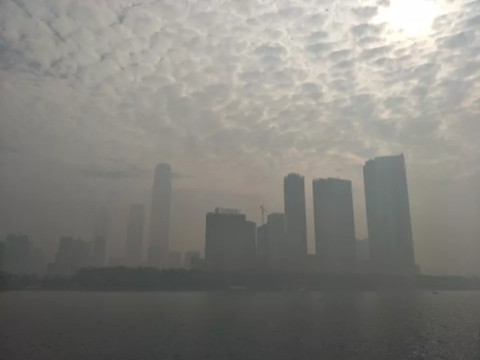
\includegraphics[width=6.67in]{images/cw1}

有人说发展的问题会在发展中解决,例如发达国家也经历过类似的阶段,但伴随产业转型与法规调控,污染问题都会自然而然地消亡;又有人说虽然城市会被雾霾笼罩,但从统计数据上看居民平均寿命其实比所谓田园风光的乡村更长;还有人说大气污染相比土壤、水还有固废污染都不算严重,只是可见度更高(也就是能见度低)\ldots{}\ldots{}的确,雾霾这个现象背后有着错综复杂的社会经济影响,从不同的角度去看会发现不一样的东西。多一个角度看问题并不会让你过的更好,但至少更明白些。

下面我将给出一些非技术与法规调控的视角,希望对读者理解雾霾以及其他一些环境污染问题能有帮助。

\subsection{研究增长的极限}

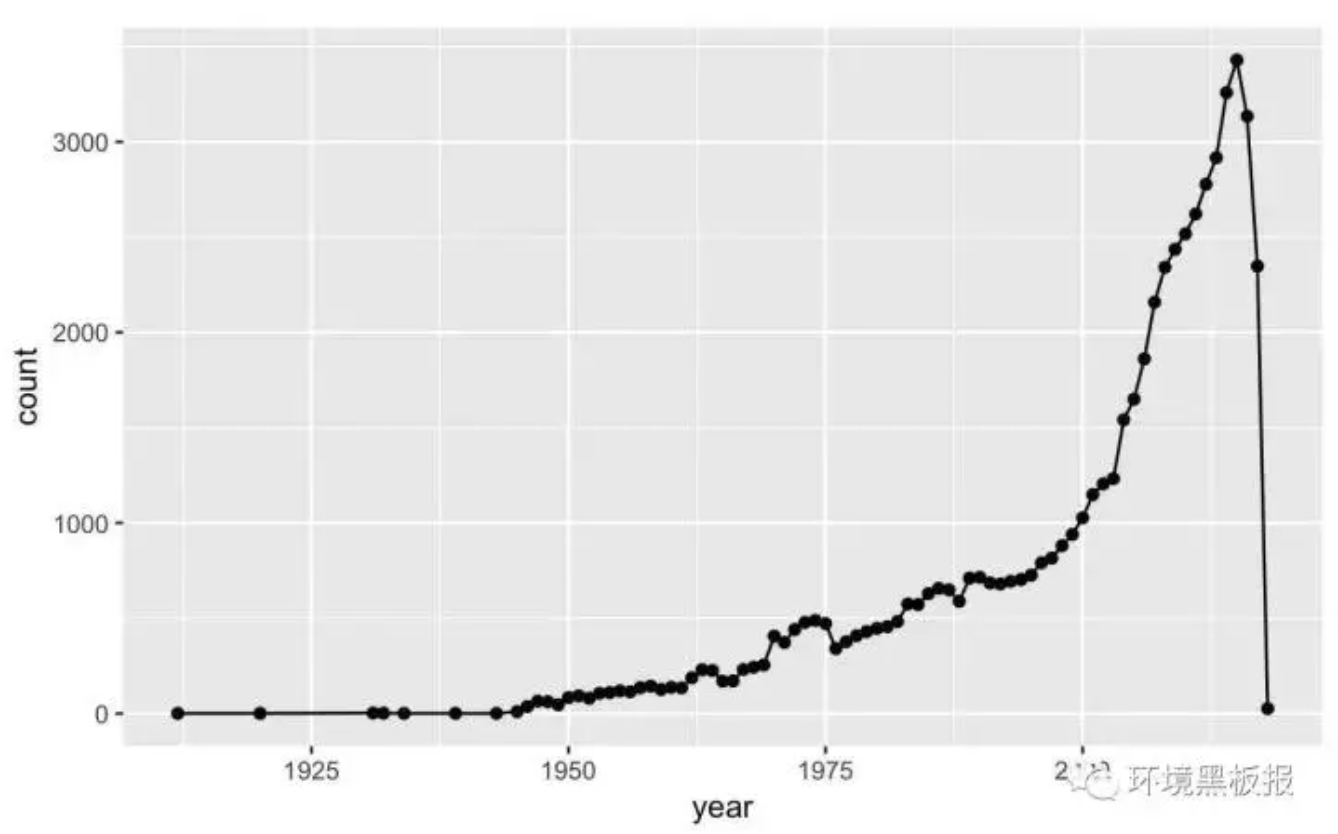
\includegraphics[width=6.67in]{images/cw2}

上图是生物资讯数据库 Pubmed 上用颗粒物(particulate
matter)作为关键词得到的论文数量,一百年来可以说是持续增长,特别是21世纪以来增长尤为迅猛。但需要注意的是到2015年达到了峰值(3429),16年已经明显下降(3134),今年还有两个月(2348),但不出意外也不会超过16年。至于为什么会有少量18年文献(26),这是学术界硬通货论文的通货膨胀,透支未来可以说是现代社会最伟大也最危险的发明,学术界亦然。也就是说,对于颗粒物的研究兴趣实际已经在降低了。

这个现象可能有点反直觉,因为近几年大气环境污染的公众关注度非常高,经费投放也很可观,但学术界却降低了学术交流频次。无独有偶,使用传统研究热点例如汞、铬、二恶英、基因组、纳米颗粒去进行检索,都会发现研究在2014-2015年间出现了峰值。但同时如果去看一些新兴研究例如3D打印,颗粒物中的细颗粒物(fine
particulate
matter),则增长还是非常迅速的(下图是以细颗粒物为关键词的文献发表状况)。

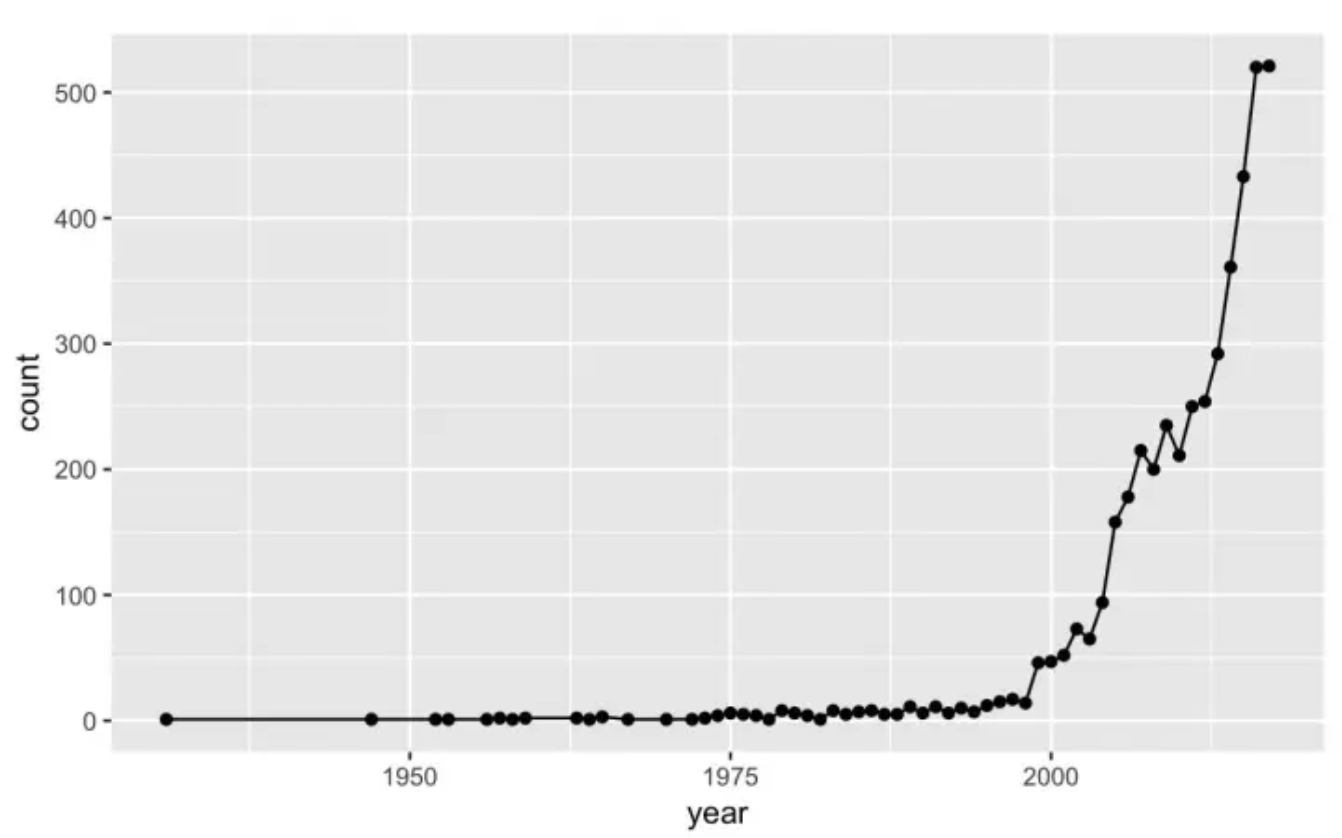
\includegraphics[width=6.67in]{images/cw3}

如果把学术界所有人的研究精力看成是总量稳定的,那么论文数可以看成精力的指标,对于包括大气颗粒物在内的很多环境研究课题而言,学术界正在把蛋糕切给更新的技术与概念。同样是进行雾霾研究,如果你从事微米尺度研究,而学术界却更加认可纳米尺度的研究,那么你的文章就很难发表,然后就是经费紧张,如此循环;进而使得新概念也不断变成老概念。

就颗粒物研究而言,目前学术圈总体关注度已经在下降,但分支中却有上升的。那么可想而知,学科内存在激烈竞争,并不是所有的颗粒物研究方向都是热点。而且还可以预期的是少数研究方向的异军突起会吸收更多学科内的研究资源,很多优秀的研究人员可能一开始选错了研究方向,最终的结局就是转行。研究的增长极限是客观存在的,所以如果你在这个年代打算去找专家咨询,最好去问上升期的新人,因为很多概念从出现到流行不到三五年,有经验的专家反而可能因为有学科内竞争关系而给出带有其自己都意识不到的感情色彩的论断。

\subsection{有原罪的雾霾}

如果某天PM2.5爆表,然后你又恰好感觉到嗓子不舒服,那么很自然你会认为这是雾霾的锅。这符合情理,但不一定符合事实,雾霾跟健康是有联系的,但跟健康有联系的可不仅仅是雾霾。即使仅仅考虑大气污染,颗粒物也只是能够产生爆表AQI的一个因素,其余的例如工业主导的硫酸型烟雾或汽车尾气主导的光化学烟雾都会影响健康,都能让嗓子不舒服,此时你会把原因归到哪里?

进一步讲,环境因素也只是影响健康的一个方面,遗传也起作用。假如你在雾霾天听到一个有气管炎家族病史的患者在咳嗽,你会认为是环境影响还是遗传作用?而根据最近Science的一份研究,即便你排除掉环境因素与遗传因素,仅仅是新陈代谢过程中DNA的复制次数就可解释癌症的发病率的66\%,而这个过程根本就无法用先天后天因素来解释,就是个生长问题。

在中国,雾霾是有原罪的,它实际承载了社会转型期人们的一部分焦虑。如果其对健康的总影响是十,那么其中真实作用可能也就二三,替遗传和其他污染物背了三四的锅,还有三四则可以说是心因性的。今年柳叶刀上一篇文献就提到,中国PM1跟PM2.5大概贡献了医院急诊的4.47\%与5.05\%。这种研究有两个问题,第一,即使排除了意外导致的急诊(例如车祸),就诊行为本身就会受天气影响;此外就是
type M
型错误(效应数量级错误),也就是说这个效应是真实的,但是影响不一定大。

这其实是目前环境研究的一个通病,找一组病人和一组正常人(有的连这个也省了)采集样本,然后一把测定几百上千种污染物(这个现在技术上是没问题的),然后算相关系数,这种情况随机你都可以发现几个的,而这样做出的发现有个通病,那就是效应通常不大,很难重现。一个小而真实的效应或许有学术价值,但舆论一放大就会产生公众心理焦虑,而心理状态又会影响生理状态,这类影响可能并不比真实影响小。

雾霾是有原罪的,但被过度聚焦了,由此产生的焦虑与恐慌本身也会产生健康影响。如果公众可以更好理解科学研究现状与其中的问题,这并不能客观降低空气污染的健康影响,但在实际意义上却可能减轻雾霾的心因性副作用。

\subsection{万金油的幻象}

不知道从什么时候开始,万金油的心态重新出现了。以前如果我告诉你有一种方法可以让你永远远离雾霾危险,你肯定说我瞎扯。好,现在我换一种说法,在人工智能+区块链+可穿戴设备+大数据的实时监控下,我可以给你一副智能眼镜,上面会实时反应你现在的风险指数,如果指数超过80\%,那么你就应该进入室内。逻辑上来说,如果你按照超过指标就躲到室内,那么这个风险永远不会变成100\%,也就是说,这跟我刚才说的永远远离雾霾危险实质等同,但是这样的产品你多半不会觉得是瞎扯,甚至会愿意付高价购买,这又是为什么?

万金油思维从来都没远离过我们,只是从熟悉的名词变成了看似专业的术语。人们有一种看起来很理性但又很荒谬的行为:乐观而盲目地相信着未知的科技。雾霾来了,那就买个最好的空气净化器;外面看不见了,那就来个3M口罩;嗓子不舒服了,那就去搞点清肺的保健品。其实很多人都知道这些科技可能还不成熟,但只要花钱了就有种事情完结可以甩锅的想法。真实的情况往往是越是大家关注的事物,就越有人去贩卖这种包装过的万金油,你买到的更多只是一个确定性的心态。

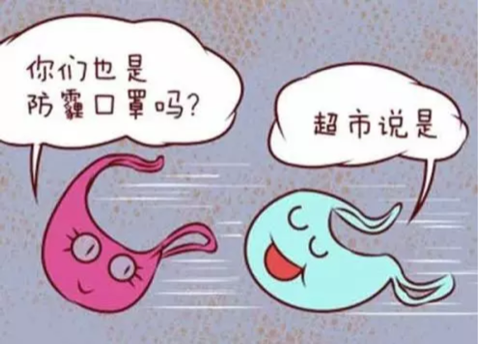
\includegraphics[width=6.67in]{images/cw4}

在这个分工细致的现代社会里,绝大多数的服务业出售的都是经过专业化包装的确定性,用来抵消分工后一颗颗螺丝钉无法感知全局的焦虑。雾霾就是个全局问题,涉及很多不同专业的知识,当个体被复杂性搞晕时,最简单的方法就是掏出一把钞票买个心安理得。即使问题不能在当前根本解决,但生活总要继续,或许这就是万金油思维在进化上的意义。在雾霾这种大IP下,科学家、政府、骗子、掮客、投机商你方唱罢我登场,过分认真你就输了。

\subsection{混沌的冬日}\label{-1}

回溯千年,宋代诗人陆游在《秋霁》中提到:``驱除云雾极知难'',除了难在技术与法规,雾霾也是直指人心的。

看看窗外,凛冬将至

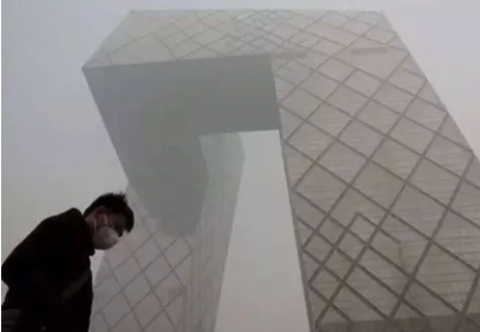
\includegraphics[width=6.67in]{images/cw5}

作者:yufree 编辑:栟

\section{北京的空气变好了,但是\ldots{}\ldots{}}

早在2009年,美国驻华大使馆便自设空气监测站,并对外发布PM2.5数据。而直到2011年以后,随着微博、微信等自媒体的蓬勃发展,一些微博大V、微信公众号开始关注并转发美国驻华大使馆的空气监测数据。这引发了公众强烈热议,什么是PM2.5也成为一时关注焦点,环保等相关政府管理部门也不得不对此有所回应。2013年,国务院发布《大气污染防治行动计划》(就是所谓的``大气十条''),提出十条具体措施,明确经过五年努力,全国空气质量总体改善。而北京随后制定了《2013-2017年清洁空气行动计划》,明确了到2017年底PM2.5年均浓度控制在60微克/立方米左右的``京60''目标。

------写在最初

今年,是``大气十条''的收官之年,北京市空气质量是否明显好转?``京60''的目标是否已经实现?带着这些问题,我们采访了北京某环境监测部门的工程师及中科院某所大气环境研究人员,并对北京市市民进行了街访。

\subsection{北京的空气质量到底变好了没有?}

北京某环境监测部门工程师(以下简称``监测部门''):从总体上来看,北京市空气质量呈现逐年转好的态势。以PM2.5为例,自2013年开展监测以来,2013-2016年PM2.5年平均浓度分别为89.5、85.9、80.6和73.0微克/立方米,下降的趋势非常明显。

根据北京市环保局发布的监测数据显示,2017年1-10月份,北京市PM2.5累计浓度为64微克/立方米,同比下降8.6\%;空气质量达标,也就是我们所说的``1级优''或``2级良''天数172天,同比增加11天。这些数据均体现了北京市空气质量正逐年好转的特征。

下图是2013年1月-2017年10月北京市PM2.5日平均浓度的热度图(单位:微克/立方米),我们可以看出,这几年,PM2.5高浓度天数确实在减少,低浓度天数在增加。

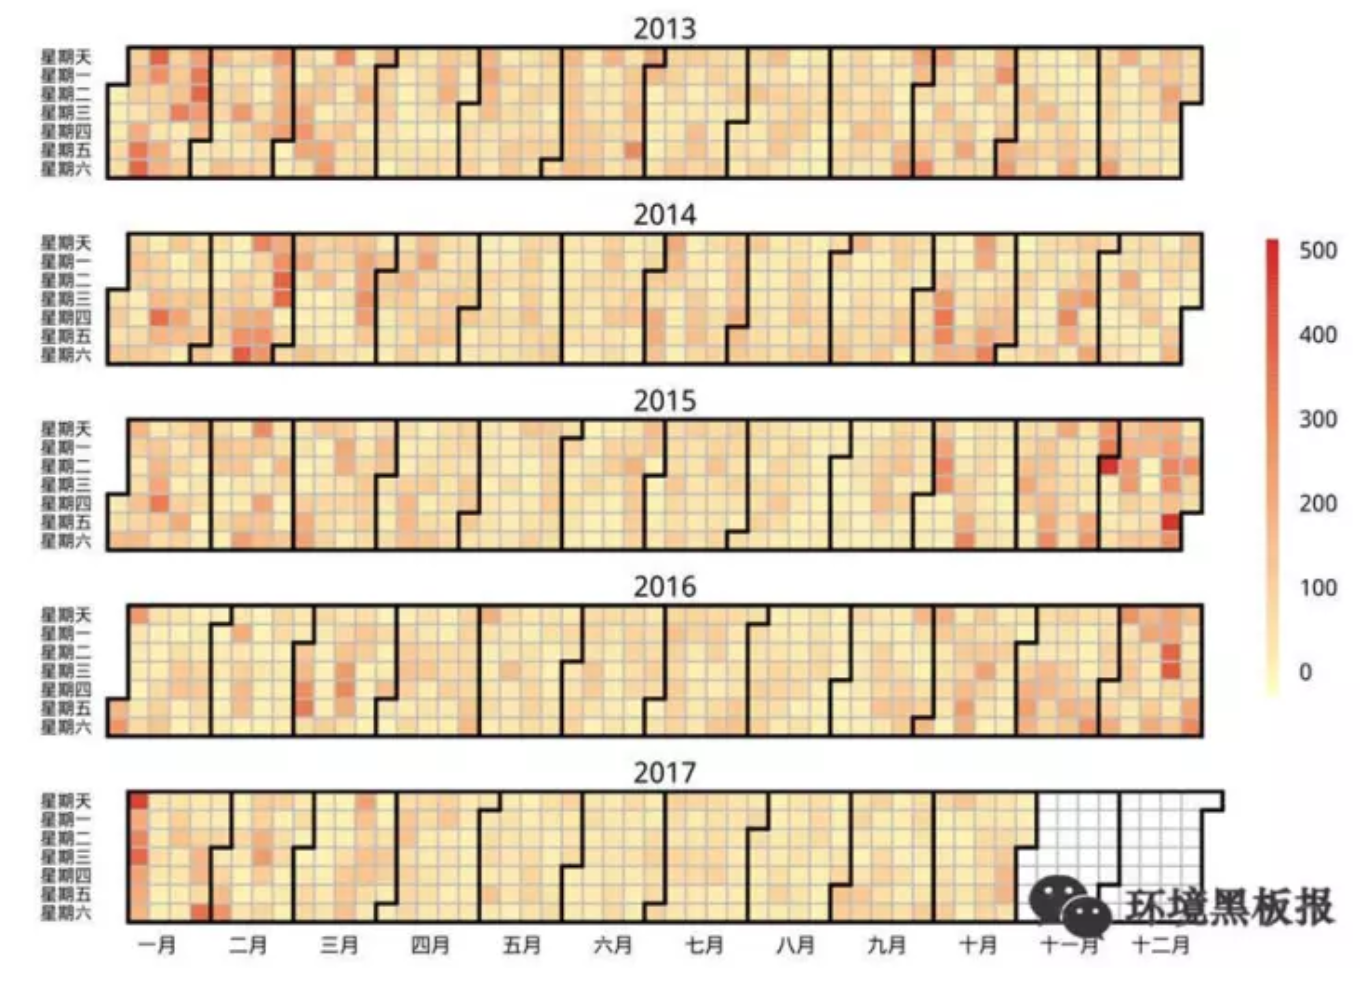
\includegraphics[width=8.33in]{images/air1}

中科院某所大气环境研究人员(以下简称``科研所''):空气质量变好还是变坏,污染物的浓度水平是一方面,污染物的成分变化更需要我们的关注。

举例来说,在1998年,北京主要遭受严重的燃煤和机动车排放混合型污染。自1998至2013年的15年期间,我们国家主要在燃煤电厂的脱硫脱硝技术方面做了很大的改进,使酸雨问题得到了控制。

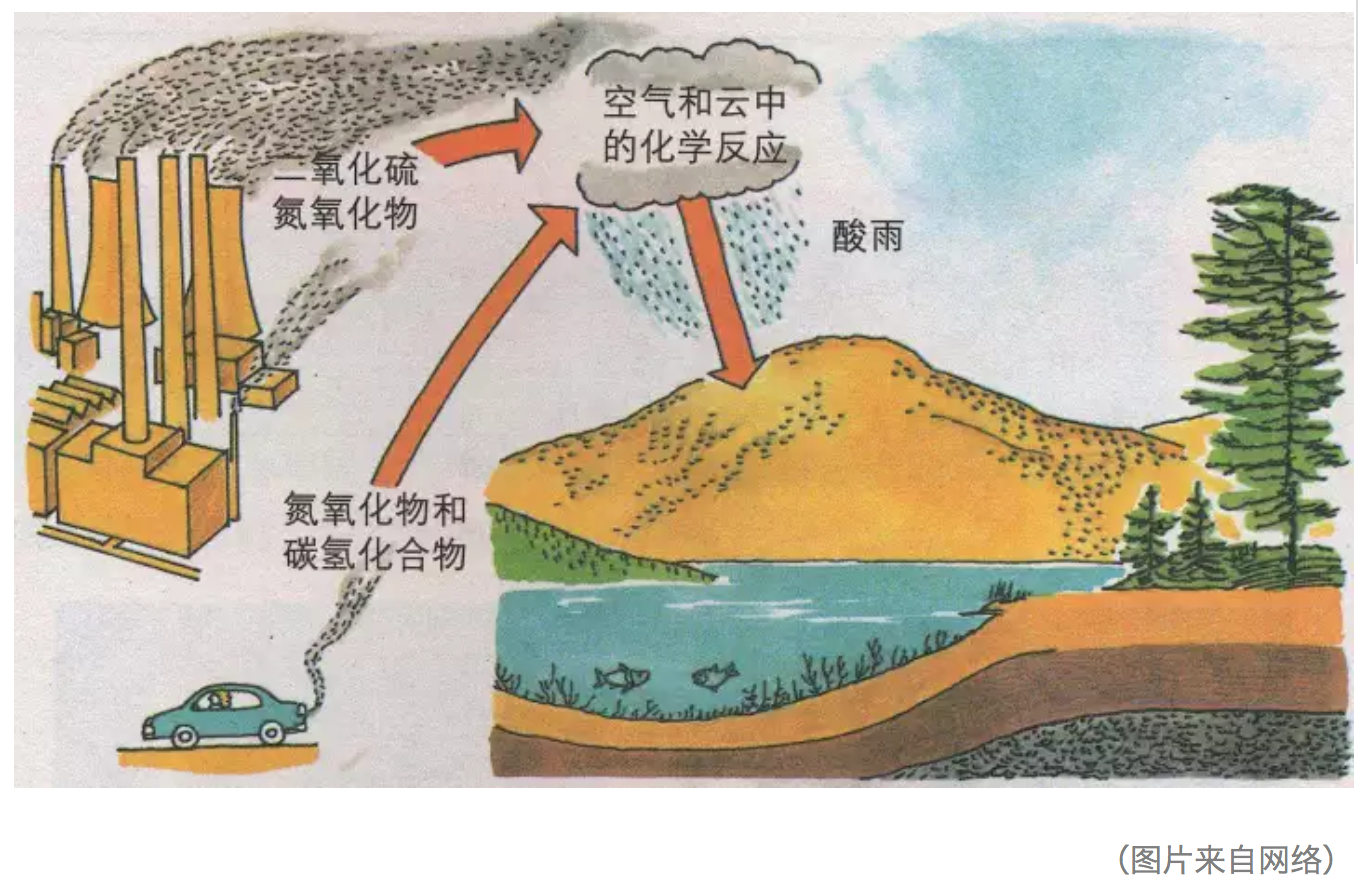
\includegraphics[width=8.33in]{images/air2}

而且,这15年期间,北京的CO、SO2、NO2和PM10的年均浓度均有显著下降,下降比例分别为58\%,78\%,24\%和42\%,尤其是CO和SO2基本稳定在国家空气质量标准值内。

但是,为什么最近几年,雾霾的问题反而更严重了呢?高效的除尘工艺只对粒径大颗粒物具有良好的去除效果,对于数量浓度较高的细小颗粒物去除率还有待提升。尤其在高湿环境下,大气中的多种污染组分如NOx、O3和光照条件促进SO2和VOC等的均相和非均相反应,促进新粒子的生成及细粒子的老化,形成成分复杂的较高浓度的细颗粒物(PM2.5)飘散在空气中,可由呼吸道直接吸入肺部,增大对人体的危害程度。同时,这些细小的颗粒物对阳光的吸收散射增强,降低大气能见度。

这几年随着环保力度加大,尤其是``大气十条''的落实,京津冀、长三角、珠三角PM2.5的浓度比2013年同期分别下降了38.2\%、31.7\%、25.6\%,下降幅度均大幅高于考核标准。``京60''目标也有望实现。

近几年,VOC的排放呈显著增长趋势,或许会成为未来大气污染治理的又一难点。

小编言:随着我们环保治理力度的不断加大,北京空气中PM2.5确实在不断减少,蓝天的数量在不断增加,我们政府下了大决心,打了场胜仗,但是空气质量是否真的变好了,可能还有待研究。

\subsection{目前,对于PM2.5浓度评价的标准使用的都是均值,如2017年,北京年均值达到60微克每/立方米左右,这样设置是否合理?}\label{pm2.5201760}

监测部门:目前的标准,使用的是均值,每日空气质量评价参考的是日均值,年度目标的完成情况参考年均值。各行各业很多和实际生产生活相关的标准都不需要特别精细化,虽然说设立置信区间能够更精细化,但是在当前的实践中可能比较有难度。标准就是个标尺作用,要满足大部分需要,在满足日常需求上,我认为用均值就够了。不过科学的标准更应该是根据人体健康效应来设置。

科研所:我不认为均值是一个很好的统计量,打个比方,如果只用一个标准值去衡量,那就相当于默认均值背后的分布或者污染特征是一样的,但实际数据的分布并不一样。如果能够精细化一些,可能会更加准确,说服力也更强一些。当然,这也是当前科研出现危机的一个例子,现实的复杂并不适合用简单统计量来描述。

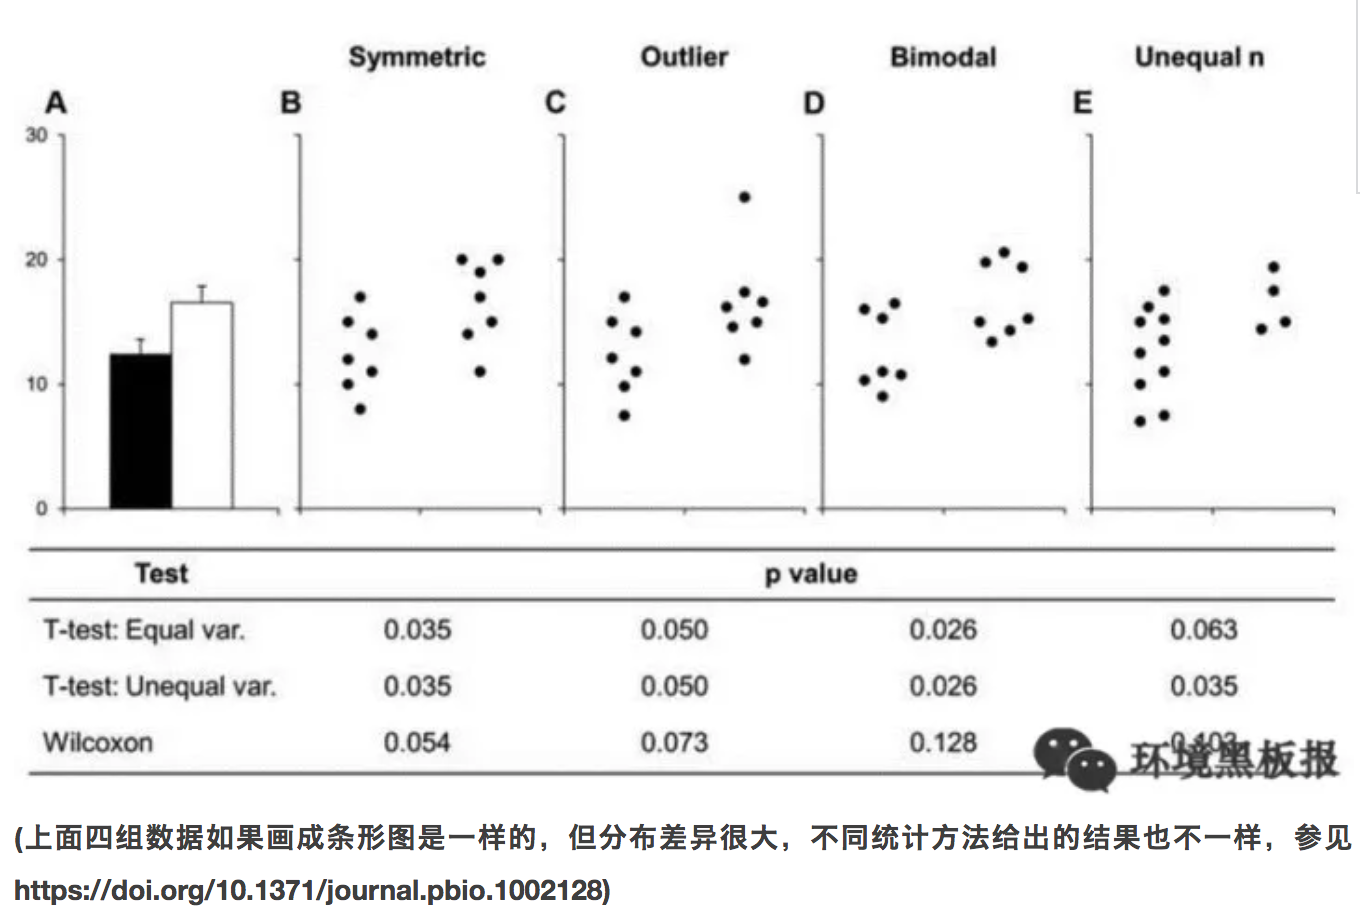
\includegraphics[width=8.33in]{images/air3}

现在环境监测能力越来越强,获得的数据越来越丰富,加上越来越先进的数据处理手段,有实现精细化展示的可能性。标准的制定最好通过置信区间来定义,例如考核指标改为90\%的分时浓度区间,也可以考虑工作日与双休日制定标准。

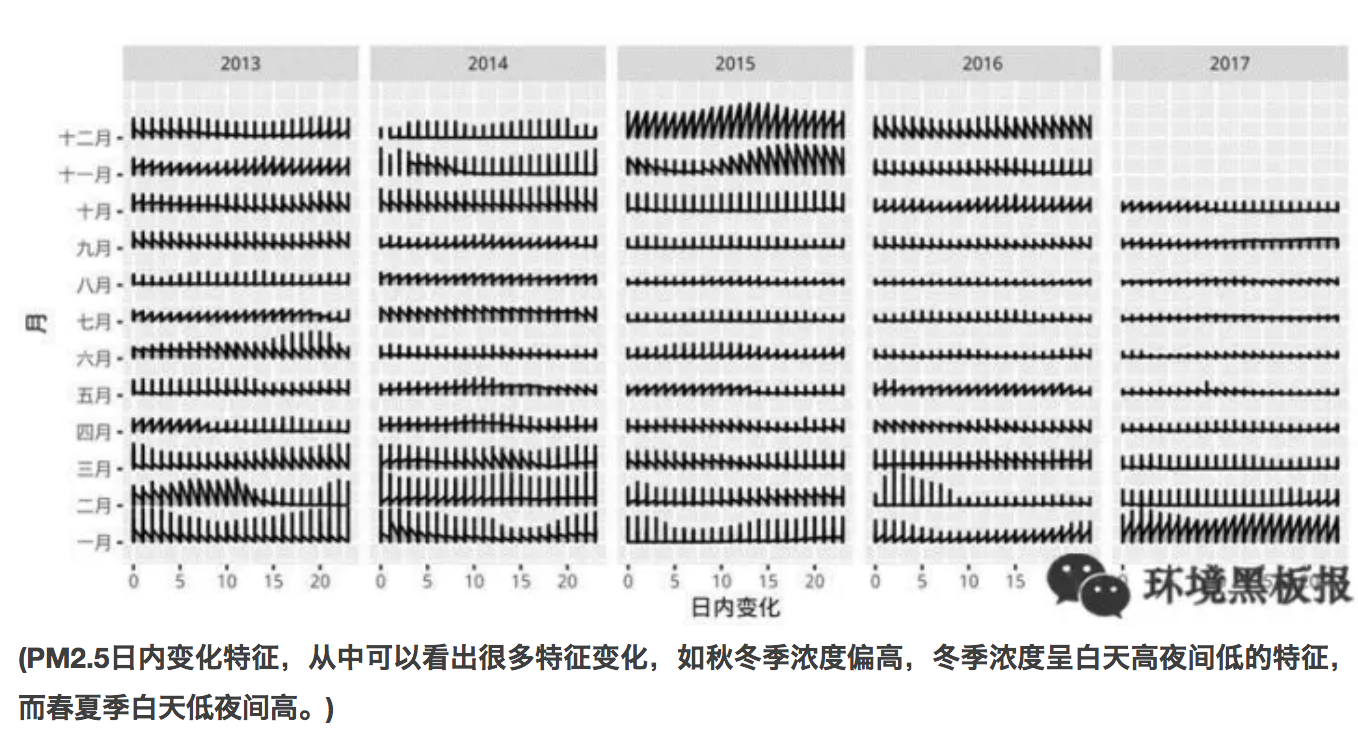
\includegraphics[width=8.33in]{images/air4}

小编言:均值作为标准,应用和管理起来或许会很方便,但是会隐含一些我们看不到的分布特征,而这些特征对于精细化管理大有裨益。

\subsection{按照《北京城市总体规划》(2016-2035年)要求,到2020年PM2.5浓度下降到56微克/立方米左右,对此,您持何种态度,判断依据?}\label{2016-20352020pm2.556}

监测部门:我对此还是持乐观态度的,主要原因为:(1)目前的高压态势环保治理已经成为常态,而不是部分时期采取的临时措施,污染源减排力度将会持续加大。(2)国家正积极加大能源结构调整,目前清洁能源的使用率和使用范围越来越大。(3)民众的环保意识越来越强,自身参与环保的行动也越来越多。在政府和民众的不懈努力下,北京市PM2.5浓度会越来越低。

科研所:对于这个观点,我持乐观态度。首先,政府、民众都很关心,科研人员也在污染源解析、气象模式预报、大气污染追因等方面做了很多的研究工作。其次,治理污染需要一个过程,在2015年以前,重点在酸雨的调控,近几年,重点在PM2.5的调控,未来还有VOC和O3问题也需要解决。根据目前的数据和政府的决心来看,我是持乐观态度的。

小编言:对于未来,我们多是持乐观态度,一方面我们对现在的政府充满了信心,``绿水青山就是金山银山''理论正在引领新实践,另一方面我们自身也深感美丽生活环境的重要性,环保意识不断增强。

听了政府监测部门和科研机构人员的回答,我们已经感受到了政府和研究机构在改善北京空气质量方面所做的努力。那么作为北京市居住的老百姓,作为空气质量改善的最直接受益人,他们的感受是怎么样的呢?

\subsection{您好,您觉得北京的空气变好了吗?}

蓝天:感觉今年蓝天确实比去年多了,是不是跟今年风多有关系啊。不过也听说最近环保搞的力度挺大,又是督察又是巡查的,空气污染严重还问责,今年还轰轰烈烈的搞了煤改气,听说周边农村里煤不让烧,气供不上,挨冻了都,好在听说环保部紧急发文,让一些没改好的地方接着烧煤。今年天儿好可能这些治理法子还是起了作用吧。

白云:感觉今年重雾霾好像是好了一点,以前雾霾严重的时候,窗户外面都几乎看不见。其实我对雾霾真是没怎么关注,感觉对自己影响不大,主要是考虑到孩子,希望每天都可以看到蓝天,这几年的雾霾让人有些麻木了吧,到哪里看到雾霾都不觉得吃惊了,反而连续出现蓝天倒是觉得不可思议。

青山:这个我还真关注了,毕竟跟咱北京人儿息息相关么。北京现在空气肯定是在慢慢变好,但是大家感觉不强烈。感觉政府宣传的不好,一方面是老百姓不信,另一方面政府没有转变思维,还是封堵,而不是疏通,预警措施也不够。

\subsection{按照目前北京市环保局网站公布数据,北京市今年很有可能达到年均值60微克每立方米左右,北京市空气质量逐年改善,您对此怎么看?}\label{60}

绿水:其实吧,我不清楚60微克是啥概念,天天听人说,也没有人科普过,如果说就是雾霾好一点,今年感觉是比去年强点,但要说强多少,也没有吧,前两天不还雾霾来着。

阳光:达标能怎样,数据可以求平均值的,总共有个30天极其严重,而其他天数全是好的,一平均不就是好了,但是老百姓的感官还是不好的。

鲜花:恩,现在政府抓环境抓的紧,我们那片好几个小工地都关了。政府立了指标,老百姓就好监督嘛。而且现在市长是搞环境出来的,又是从环保部过来的,我觉得在改善北京空气方面,还是能有所作为的。

小编言:看来,民众的感受也是因人而异啊,不过总的来说,政府的努力还是得到了认可,民众提出质疑的同时也对政府对科研部门寄予了厚望。

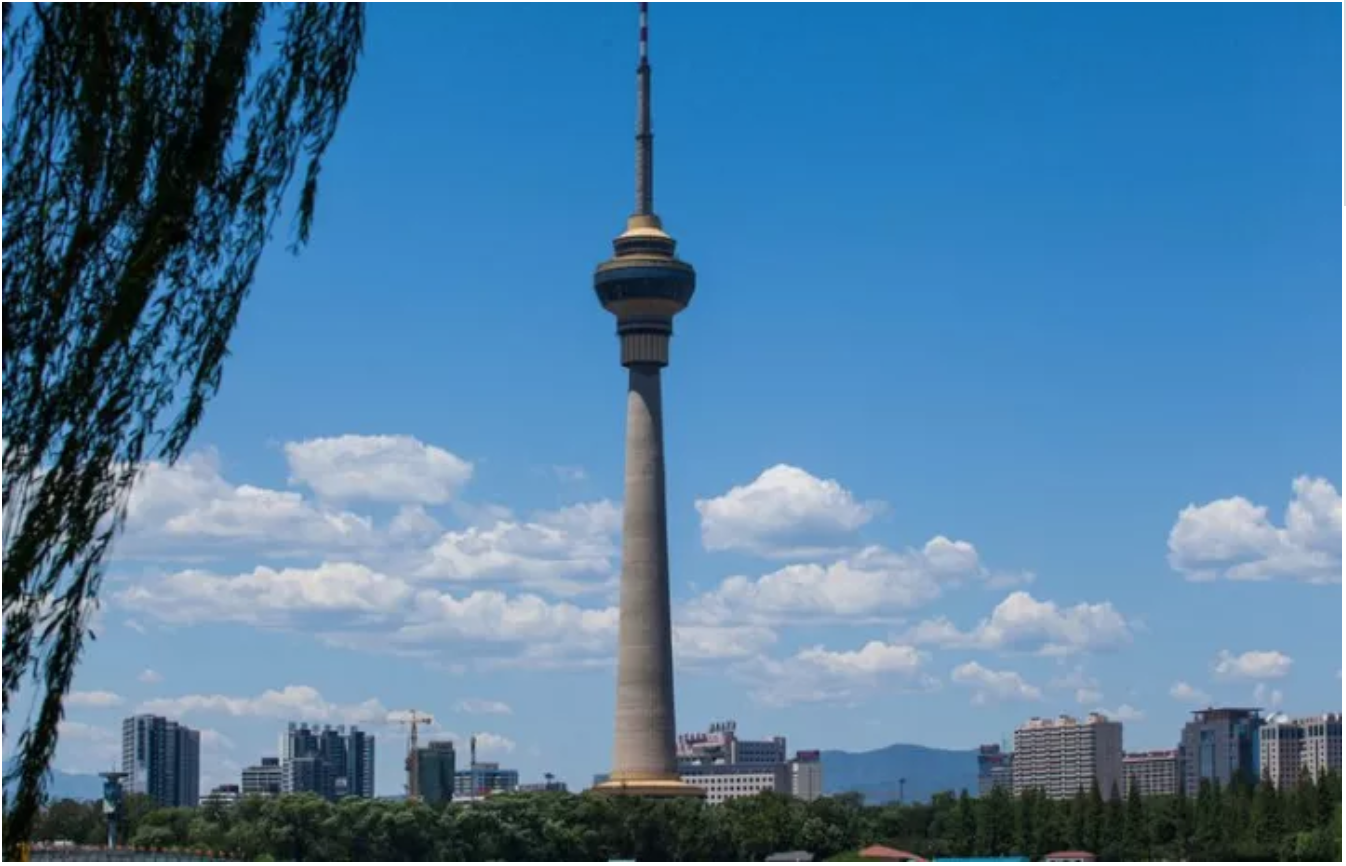
\includegraphics[width=8.33in]{images/air5}

经过几年的努力,北京的空气改善明显,但是否有新形式的污染物出现危害公众健康,是否在目前认为的质量改善背后隐藏着其他的隐患,作为政府工作人员还是科研工作者亦或是你我,都仍需负重前行,不忘初心。

作者: 次要男主角 校稿:周宁,王小咖 图片:yufree 编辑:竹而乐

\section{等风来}

2000年左右,北京人讨厌风,因为一到大风季节,黄沙滚滚,遮天蔽日。可是近些年来,人们又盼着风,期望风来了,把自己从雾霾中解救出来,一时间``等风来''成了所有人的心声。雾霾和风几乎每年都会在北京的地界干上几场大仗,有时力量悬殊,战争迅速结束;有时势均力敌,展开拉锯战。下面我们详细解析一下双方斗争的形势。

\subsection{与雾霾的战争}

首先我们将北京全市PM2.5(细颗粒物)日平均浓度高于200微克/立方米、持续时间超过2小时的污染状况定义为一次重污染事件,2013年8月到2014年8月期间,我们共观察到六次重污染事件,分别为2013年10月28日(265.59微克/立方米)、2013年12月8日(202.63微克/立方米)、2014年1月23日(233.71微克/立方米)、2014年2月15日(437.15微克/立方米)、2014年2月26日(337.39微克/立方米)和2014年3月27日(234.32微克/立方米)。我们基于GIS软件,通过克里金差值方法对这六次重污染过程形成和消散过程进行了模拟。

\subsection{雾霾的胜利}

北京PM2.5重污染事件主要受外源传输影响。从重污染形成的过程看,北京这六次重污染过程中,细颗粒物从北京东南部或者南部,逐渐向城中心和西北部缓慢扩散,最终全城形成重污染(图1)。

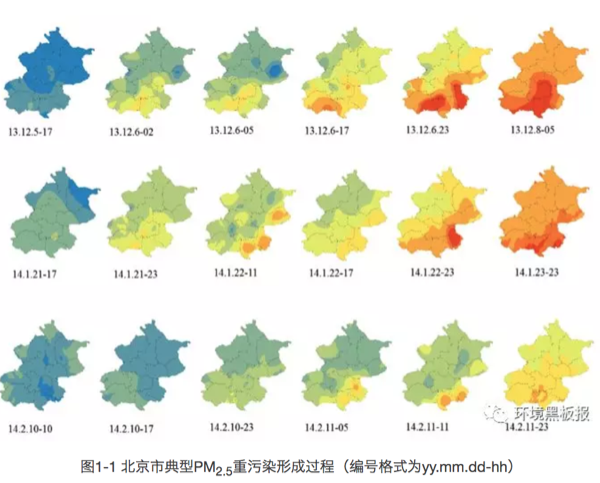
\includegraphics[width=8.33in]{images/windhaze1}

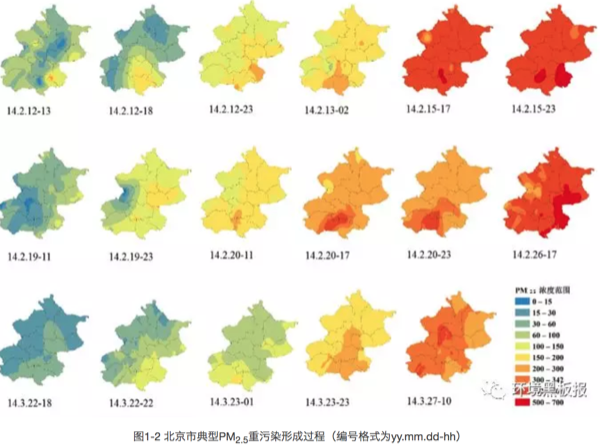
\includegraphics[width=8.33in]{images/windhaze2}

在重污染形成期间北京平均风速低于1米/秒,主导风向为南风和东南风(图2),说明北京的PM2.5重污染的形成受外源传输影响较大。主要的污染物来自北京东南部和南部的廊坊、天津和保定等省市。重污染的形成时间一般为3-7天。

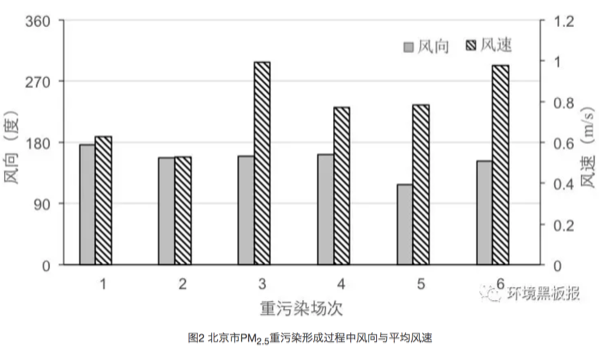
\includegraphics[width=8.33in]{images/windhaze3}

\subsection{大风的胜利}

北京PM2.5重污染的消散主要借助风。北京这六次重污染消散过程中,受风的影响,细颗粒物从北京西北部开始,逐渐向城中心和东南部推移,最终实现全城PM2.5消散(图3)。在此期间北京平均风速为2.5米/秒,而主导风向为西北风和北风为主,只有一次为南风。从模拟结果看,北京的细颗粒物被西北风一分为二,之后在向东北和西南逐渐扩散,直至完全消散。说明北京的PM2.5重污染的消散主要依赖于西北风的影响,而且平均风力为2.5米/秒(图4)。重污染的消散过程比较迅速,整个消散过程时间一般在6-11个小时,其中消散最快的一次,出现在2014年2月26日,全市平均PM2.5浓度从431微克/立方米降到21微克/立方米,仅用了6个小时,期间平均风速为3.2
米/秒,主导风向为西北风。其中最慢的一次(2014年2月17日)持续了18个小时。主导风向为东南风,风力2.4米/秒。可见,北京PM2.5的消散过程与风向和风力有密切关系。

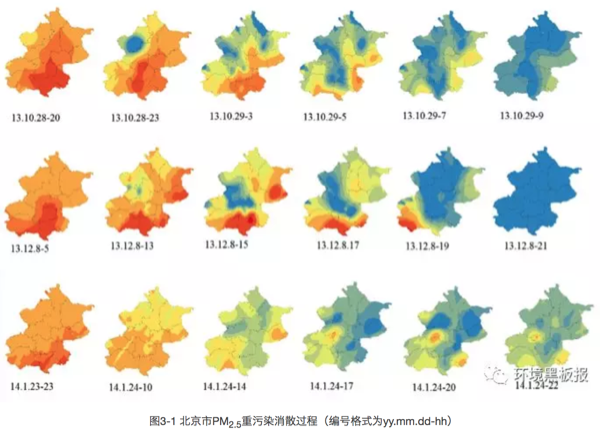
\includegraphics[width=8.33in]{images/windhaze4}

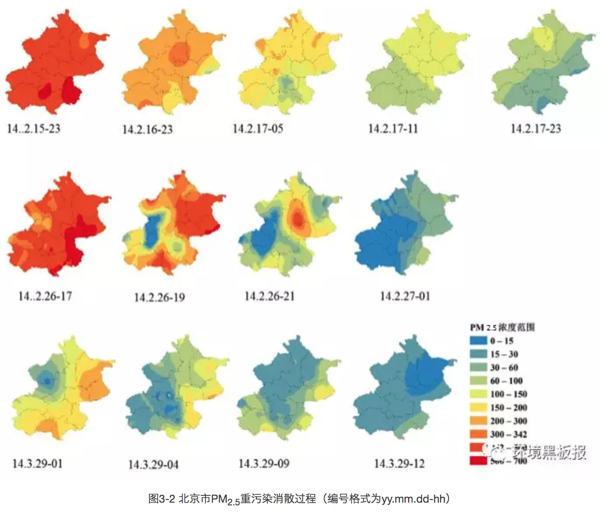
\includegraphics[width=8.33in]{images/windhaze5}

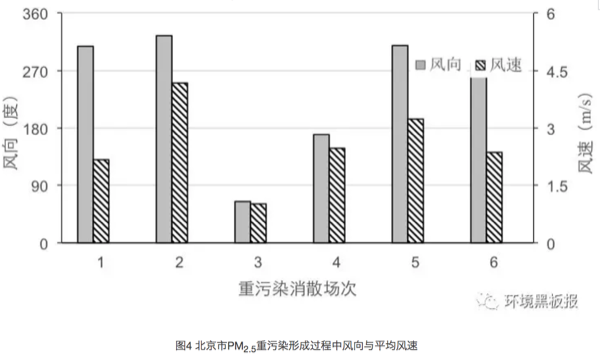
\includegraphics[width=8.33in]{images/windhaze6}

总体看来,风速1米/秒是一个坎,风速小于1米/秒,则容易形成雾霾累积;当风速大于1米/秒,重污染容易扩散,尤其是西北风。

\subsection{势均力敌}

2018年1月13-17日,京津冀及周边地区经历了一次大范围重污染过程,污染范围包括河北省、山西省、山东省和河南省等城市全部或者部分地区。石家庄市是受重污染影响较大的城市之一,截止到1月21日0时,本次中污染石家庄市出现了164个小时的重度污染和90个小时严重污染(数据来源于网络,未经审核)。

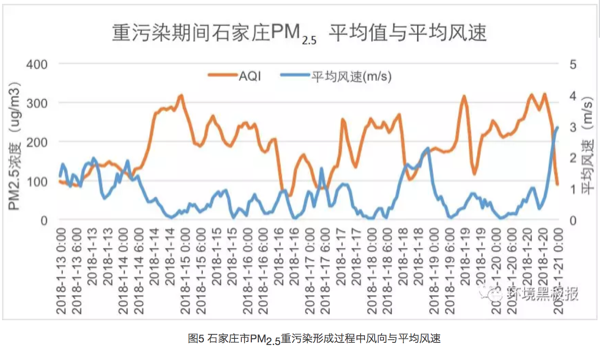
\includegraphics[width=8.33in]{images/windhaze7}

石家庄市从13日凌晨开始空气质量逐步转差,污染物浓度波动上升(图5)。13日5时达到重度污染,
14日6时,污染物逐渐累积,11时达到严重污染。16日14时至17日7时空气质量出现短时改善,部分时段降至中度污染以下水平。此后空气质量继续恶化,重污染持续,但污染程度轻于第一次累积过程。1月18日15时,再次得到短时缓解,之后污染物浓度继续升高,全市PM2.5小时平均值最高值出现在19日12时,达到317微克/立方米。之后迅速下降。1月19日16时,下降到最低值,为117微克/立方米。之后污染物继续累积,1月21日空气质量好转。截止到目前,重污染源已经持续393个小时,其中,有164个小时的重度污染和90个小时严重污染(数据来源于网络,未经审核)。

在此过程中,风速与空气污染指数呈现明显的负相关关系(图5)。风与霾此消彼长,在石家庄市展开拉锯战,持续时间已经超过一周。中间几次过程,主要风速大于1米/秒,空气污染就会得到改善。一旦面临静风时刻,污染物开始逐渐累积。

\subsection{雾霾攻坚---源头把控}

在污染治理上,我们要做的还有很多,默默的等风来,不是真正的解决问题的方法。根据贺克斌院士的观点,城市治霾的根本在于管住污染源。2017年8月18日《京津冀及周边地区2017-2018年秋冬季大气污染综合治理攻坚行动方案》(环大气〔2017〕110号)实施以来,在京津冀及周边地区2+26城市,坚持问题导向,把稳固``散乱污''企业及集群综合整治成果和高架源稳定达标排放作为坚守阵地,把压煤减排、提标改造、错峰生产作为主攻方向,把重污染天气妥善应对作为重要突破口,加强联防联控,严格执法监管,强化督察问责,全面实施攻坚行动,动员全民共同应对重污染天气。``攻坚行动''方案规定主要完成的11项任务中有8项与污染源管控有关。截止到2017年12月PM2.5浓度削减幅度最大的前六位城市是石家庄、北京、廊坊、保定、鹤壁和安阳市,与去年同期相比,PM2.5浓度削减幅度均在40\%以上,可见污染源管控才是真正解决雾霾的根本手段。

等风来不如去追风,幸福都是奋斗出来的,总有一天我们能切实做到污染源有效管控,从源头上减少排放,雾霾问题才能从根本上得到解决,相信我们生活的环境会越来越好。

作者:大石 校稿:看透,胜利屯屯长 编辑:丫头晚安

\section{纳米非米}

随着``水十条''、``气十条''和``土十条''的出台,我国已全面启动了``向污染宣战''的环境大战。那么纳米材料如何在环保领域掀起新潮呢?本文以碳纳米材料为一个视角,从选料-制备-应用的角度浅谈一下纳米材料在环保领域如何小试牛刀。

\subsection{碳纳米材料}

相信在很多读者的印象中,``纳米(Nanometer)''一词总是披着神秘的面纱,影影绰绰,忽远忽近。那么纳米到底是什么?实际上,它与毫米、厘米和分米一样,也就是个长度单位而已,十亿分之一米,即一纳米。

纳米尺度的物质在性质上,跟宏观物体表现出巨大的差异。比如纳米级的金子不再是金色而会失去光泽呈现黑色,纳米级的导电体会变得绝缘,坚硬的金属在纳米级会变得柔软。实际上,无论是人工纳米材料还是天然纳米材料,我们经常与它们亲密接触。大家几乎天天使用的数码电子产品的中央处理器就是用纳米材料制备;iphone的疏油涂层、国家大剧院的穹顶都与纳米材料有关;军事里的隐形战机也是涂了一层吸波纳米材料;甚至大气里的雾霾也包含了各种尺寸的纳米颗粒。可以说纳米材料已经与我们的生活息息相关了。

碳纳米材料的重要性和应用潜力已在最近20年的最高科学奖项中得到承认,包括1996年诺贝尔化学奖(富勒烯)、2008年卡弗里奖(碳纳米管)和2010年诺贝尔物理学奖(石墨烯)。由于其独特的理化性质,碳纳米材料在环境治理领域的应用研究一直是热点之一。然而由于目前的碳纳米材料制备方法成本高、产率低、条件苛刻、生产过程会伴有有毒副产物,极大地限制了其在环境领域的实际应用。因此,迫切需要开发高效、绿色、低成本的材料制备技术。在此背景下,该领域里近年来兴起的``以废治废''新概念逐渐引起了注意。意即将人们通常视作废弃物的材料(如富碳生物质)加工处理成碳材料,再投入到环保相关领域里使用。

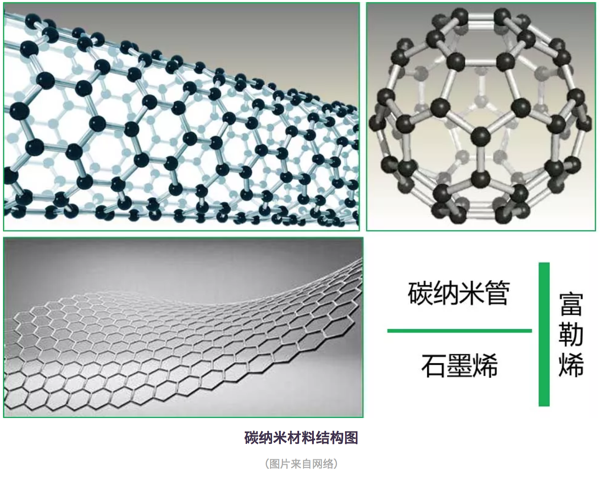
\includegraphics[width=8.33in]{images/nano1}

\subsection{哪些废弃物可以加工成纳米碳材料?}

一般来讲,可以加工成纳米碳材料的废弃物,可以按其环境价值分为两类。一是低值类废弃物。如秸秆、稻草、稻壳等植物类废弃物;动物粪便、剩余污泥等有机质废弃物;以及甘蔗渣、甜菜渣等工业废弃物;二是负值类废弃物,如塑料袋、塑料瓶、海绵、轮胎等。

这两类的大多数废弃物都未得到合理利用,以此类废弃物作为原料制备碳纳米材料,一方面可以降低大规模生产时的成本,另一方面也可解决传统处置方式可能引起的环境污染问题。例如我国农村地区的秸秆(环境黑板报后续会有关于农村秸秆的专题文章)和农膜问题,大量焚烧会造成严重的空气污染和资源浪费。

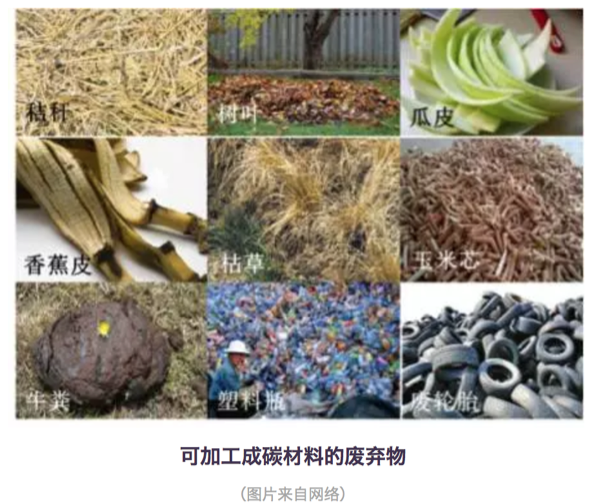
\includegraphics[width=8.33in]{images/nano2}

\subsection{如何将废弃物加工成纳米碳材料?}

一般有水热碳化法和直接碳化法。

水热碳化法是指在密闭环境中,以水溶液为介质,使原料在高温(100-300°C)高压下经过一系列复杂反应生成碳材料的过程(实际上就是将原料洗好、称好,放铁罐子里扔烘箱里反应半天左右就行)。用水热碳化法制备碳材料,因其操作简单、无污染、对仪器要求低、转化率高等优点被广泛应用。此外,水热法合成的碳材料表面通常会含有丰富的官能团,特别有利于其应用在工业废水的处理中。目前,包括木屑、树叶、稻壳、松针、塑料袋、废报纸等废弃物都被成功地通过水热法碳化成碳材料,还有研究通过此法成功地将草变成了荧光碳量子点。

直接碳化法是指将原料置于无氧条件(惰性气体)下,高温(\textgreater{}600°C)裂解成碳材料的过程。(实际上也很简单,就是将原料放到管式炉中通氮气或者氩气加热一段时间就可以)在高温条件下,原料中的挥发性有机物会逐渐被分解直至留下碳骨架。通常,直接碳化法还需加入一些化学活化剂或者氧化性气体来活化碳材料,以使其表面孔隙度和比表面积增强。碳化温度、升温速率、碳化时间等因素都会影响碳材料最终的形貌和性质。用此法合成的碳材料,表面会具有较强的疏水性,所以对有机污染物的吸附能力很强。

\subsection{纳米碳材料在环保领域有哪些用处?}

\begin{enumerate}
\def\labelenumi{\arabic{enumi}.}
\tightlist
\item
  土壤修复
\end{enumerate}

以废弃生物质制得的碳材料具有发达的孔隙结构,当被添加到土壤中时,可以明显改善土壤结构,降低土壤的体积质量\href{陈心想,耿增超。西北农林科技大学学报(自然科学版),2013,41:\%20167-174.}{1}。另外,生物质以生物质碳材料的形式贮存在土壤中,C元素被固定,减少了向大气的排放;另一方面,生物质碳材料也可以为土壤提供N等营养元素,提升土壤肥力\href{Kezhen\%20Qian,\%20Ajay\%20Kumar,\%20et.al.\%20Renew.\%20and\%20Sustain.\%20Energy\%20Reviews,\%202015,\%2042:\%201055-1064.}{2}。上海交大曹心德教授认为生物质碳材料还可以用于土壤污染物的稳定化修复,他将具有独特吸附性能的碳材料形象比喻为``吸盘'',对土壤中重金属和有机污染物进行吸附``封锁'',从而阻碍植物对污染物的吸收。Puga
A. P.等人将甘蔗秸秆制成碳材料用于土壤中重金属钝化研究,发现其可将Cd、Pb
和 Zn 的有效态分别降低 56\%、50\% 和
54\%,并抑制它们向地上部的迁移\href{Puga\%20A\%20P,\%20Abreu\%20C\%20A,\%20et\%20al.\%20J.\%20of\%20Environ.\%20Manage.,\%202015,\%20159:\%2086–93.}{3}。Khan.
S.等人使用盆栽试验研究证实,
用污泥制得的碳材料能够减少水稻对As、Co、Cr、Cu、Ni、Pb的吸收\href{Khan\%20S,\%20Cai\%20Chao,\%20et\%20al.\%20Environ.\%20Sci.\%20\&\%20Technol.,\%202013,\%2047\%20:\%208624-8632.}{4}。当然,不同的废弃物原材料、碳化温度、碳化方法制得的碳材料物理化学性质不同,其土壤修复的效果也有差异。

\begin{enumerate}
\def\labelenumi{\arabic{enumi}.}
\setcounter{enumi}{1}
\tightlist
\item
  污水处理
\end{enumerate}

废水中常见的污染物有重金属离子、染料及其他有机污染物。吸附法处理废水由于工艺简单、成本较低、可利用吸附剂来源广泛等优势倍受青睐。废弃物加工制得的碳材料比表面积大、孔隙度高、表面基团丰富,对吸附废水中的污染物十分有利。研究表明,以废弃物为原料制得的碳材料不仅可以通过表面作用(静电吸引、疏水作用、π-π作用等)对重金属离子和有机物分子进行吸附(adsorption),还能凭借较高的孔隙度对油类污染物进行吸收(absorption)。例如新加坡南阳理工大学张华教授课题组成功将废报纸制得碳气溶胶材料用于油类物质和有机溶剂如氯仿等的去除,取得了较好的处理效果\href{Bi\%20H,\%20Huang\%20X,\%20et\%20al.\%20Small\%202014,\%2010,\%203544.}{5},这为解决海洋原油泄露污染提供了一个潜在的解决思路。印度理工学院鲁尔基分校Vinod
K.教授将废轮胎制得的碳材料作为吸附剂处理水中重金属离子,发现其对Pb2+、Ni2+有非常好的吸附能力\href{Gupta\%20V\%20K,\%20Ganjali\%20M\%20R,\%20et\%20al.\%20Chemical\%20Engineering\%20Journal,\%202012,\%20197:\%20330.}{6}。陕西师范大学张志琪教授课题组成功将香蕉皮碳化为多空碳材料,发现其对水中典型染料分子亚甲基蓝有较好的吸附去除能力\href{Liu\%20R\%20L,\%20Liu\%20Y,\%20et\%20al.\%20Bioresourse\%20Technology\%202014,\%20154:\%20138.}{7}。

\begin{enumerate}
\def\labelenumi{\arabic{enumi}.}
\setcounter{enumi}{2}
\tightlist
\item
  能源应用
\end{enumerate}

此种碳材料由于较高的石墨化程度,其电子传递能力较强。又由于生物质中还有大量的N,P,S等杂原子,使得由其制备的碳材料导电性进一步增强。因此此种材料在电化学上也具有广阔的应用前景。例如碳材料因为比表面积大、稳定性好、导电性好、价格便宜、来源丰富而成为超级电容器电极材料的首选。我们日常生活中的新能源汽车、数码相机,甚至楼道应急灯都有超级电容器的身影。例如大连理工大学邱介山教授课题组将虾皮制备成氮掺杂碳材料用作超级电容器,其在电流密度为50
mA/g时,比电容可达357
F/g\href{Gao\%20F,Qu\%20J\%20Y,\%20et\%20al.\%20Electrochim.\%20Acta\%202016,\%20190:\%201134.}{8}。利用西瓜皮、麦秸、绿茶、柚子皮、稻壳等制成的碳材料也可作为性能优异的负极材料用于锂离子电池。例如新加坡南洋理工大学于霆教授将竹筷碳化成碳纤维用于锂离子电池,其首次放电和充电质量比容量值分别为500mAh/g和283
mAh/g,且循环稳定性较好,有望替代传统石墨电极在锂电池中的作用\href{Jiang\%20J,\%20Zhu\%20J\%20H,\%20et\%20al.\%20Energy\%20Environ.\%20Sci.\%202014,\%207:\%202670.}{9}。

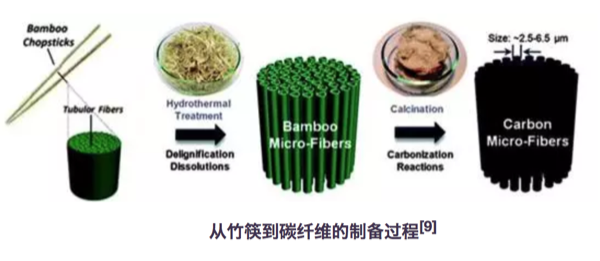
\includegraphics[width=8.33in]{images/nano3}

\subsection{结语}

以废弃物为原料制备的碳材料已被广泛研究用于土壤修复、污水处理和电化学领域,展现出了广阔的潜在应用前景。废弃物来源广泛、价格低廉的性质也使得此概念为大规模商业生产提供可能。然而目前对废弃物碳材料的研究才刚刚起步,处于发展阶段,很多碳材料仅限于实验室制备而没有进行大规模的工业化生产,距离大规模实际应用还为时尚早。

此外,在大规模应用之前,其对环境可能造成的潜在风险也有待进一步研究。这也正是纳米科技目前的发展缩影。正如中国科学院院长白春礼所说:``纳米科技发展方兴未艾,基础科学研究领域中新原理不断建立、新功能材料的涌现与可控制备技术的发展、纳米生物医药的应用探索都体现出纳米科技对人类知识体系的极大拓展以及对生活方式的潜在推动作用。尽管纳米材料显示了产业化以及临床应用的巨大前景,但多数材料目前仍处于实验室研究阶段,如何实现这些材料的功能化、推动商业化应用、相关的生态影响和生物效应是纳米科技发展面临的关键问题''。中国科学院生态环境研究中心江桂斌院士曾将基础研究形象比作翻书:``当书本一页一页翻至最后时,就是量变到质变的时候''。这也同样适用于纳米领域,或许质变之时我们就能用上充电几秒即可充满的电子产品,纳米机器人实现药物精准输送、有的放矢。

文献引用

作者:眼神防守 校稿:柴胡半夏苏,yufree 编辑:栟

\section{\texorpdfstring{你喝的可能是``有毒''的自来水?!}{你喝的可能是有毒的自来水?!}}

\subsection{水发生了什么?------水污染}

地球是个名副其实的``水球'',水资源总储量约为1.36×109km3,但除去海洋等咸水资源外,只有2.5\%为淡水。淡水又主要以冰川和深层地下水的形式存在,储存在河流湖泊中能被人类所利用的淡水仅占全世界总储水量的0.3\%,
然而,这极为稀有的淡水,却面临着另外一个不可忽视的严峻问题------水污染。水污染问题使得人类``获得安全可靠的饮用水''这一基本诉求难上加难。

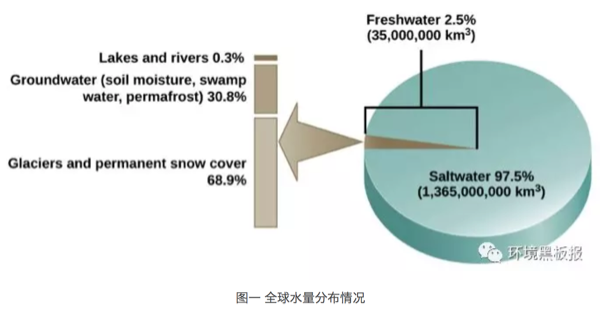
\includegraphics[width=8.33in]{images/dushui1}

联合国组织秘书长在2002年世界水日发布的新闻稿估计,
全世界有11亿人无法获得安全饮用水。中国的水污染问题尤其严重,如图所示,中国绝大部分地区的饮用水仅满足最低标准,在中南部有些地区,饮用水水质更加糟糕。

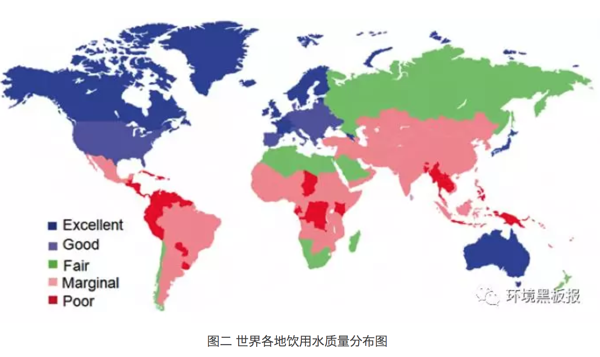
\includegraphics[width=8.33in]{images/dushui2}

\subsection{引起水污染的罪魁祸首是谁?------污染物}

近些年来,全国各地水污染事件频发,如2012年12月,位于山西省长治市境内的煤化工厂发生苯胺泄漏入河事件,导致河北省邯郸市发生停水和居民抢购瓶装水,同时由于泄漏苯胺已随河水流出省外,河流下游的河南省安阳市境内红旗渠等部分水体亦检出超标的苯胺、挥发酚等污染物。

综合所有水污染事件可得出,引起水污染的污染物有很多,通常可分为三大类,即物理性、化学性和生物性污染物。

物理性污染物包括悬浮物、热污染物和放射性污染物。其中放射性污染物危害最大,
但一般存在于局部地区。化学性污染物包括有机和无机化合物,
该类化合物近些年来在环境水体中频繁被检出。生物性污染物包括细菌、病毒和寄生虫。随着痕量分析技术的发展,至今从源水中检出的化学性污染物已达数千种以上。在所有的化学性污染物中,微量有机污染物逐渐引起人们的广泛关注,并已成为世界几乎所有地区水污染的首要污染物。

微量污染物是指那些广泛使用但通常在很低或者极低浓度水平就能影响自然环境生物化学过程的有机污染物,包括人工化学合成品,比如活性药物成分、食品添加剂、化妆品成分和洗涤剂成分,以及天然存在的一些物质如激素、生物毒素等。近年来,一些新型微量污染物,例如药物与个人护理品(PPCPs)、内分泌干扰物(EDCs)、全氟类化合物(PFCs)等的环境污染及潜在影响问题已成为各国学者和公众关注的焦点。很多微量污染物具有较强的环境持久性、生物活性、生物累积性和难降解性,如果长期暴露于环境中,对生态系统和人类健康将带来难以预测的潜在风险。我国是各类工业品、药品的生产和消耗大国,工业和人口密集,能源和资源利用率仍然较低,高强度的工业化学品生产、使用和废弃会产生严重的环境效应,因此微量污染物的环境残留问题更是不容忽视。

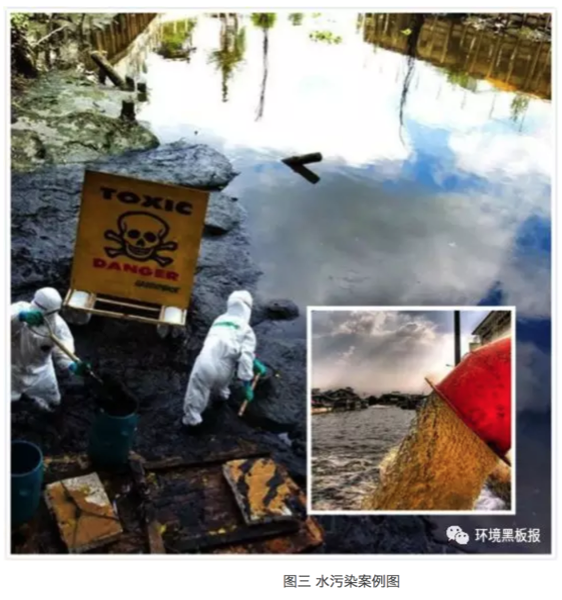
\includegraphics[width=7.81in]{images/dushui3}

\subsection{污水处理厂可以使水变干净么?------未必!}

为了去除环境水体中的微量污染物,人们寄希望于现有的污水处理工艺。然而,当被污染的水经过污水处理厂处理之后,真的可以变干净么?答案却是未必!

\begin{itemize}
\tightlist
\item
  微量污染物的去除很难达到100\%
\end{itemize}

近年来,欧盟和一些发达国家开始高度关注水环境中的微量污染物问题,研究发现城市污水中化学物质普遍存在,有些是常规污水处理工艺难以去除的,因此污水排放是河流水体中化学物质的重要来源。

城镇污水处理厂的工艺选择主要基于排放标准中COD、BOD5、NH3-N、TN、TP等常规污染物指标的稳定达标。另外值得注意的一点是,污水中的许多痕量污染物具有一定的毒性,对活性污泥中的微生物易产生一定的抵抗和抑制作用,因此,目前常用的污水处理工艺如活性污泥等对痕量污染物的去除并不能达到100\%。同时,在污水处理工艺流程中,部分微量污染物通过活性污泥吸附或者生物降解、水解等得到去除,但许多亲水性物质不能吸附到活性污泥上,导致出水仍然残留相对较高的浓度,释放到接纳水体中,引起水生生物的慢性接触。需要关注的是,某些微量污染物具有中等或较强的疏水性,易于被活性污泥絮凝吸附;但由于仅仅是相的转移而不是降解,这部分被吸附的微量污染物往往随着污泥的处理处置过程进入地表水体或土壤环境中,直接或间接造成潜在的环境与健康风险。城镇污水处理厂出水及污泥是环境中不可忽视的痕量有机污染物的源。

\begin{itemize}
\tightlist
\item
  残存的微量污染物可能在处理过程中发生二次反应生成更毒的物质
\end{itemize}

在当前的污水处理厂中,化学降解方法包括光催化氧化,臭氧化和氯化被认为是有效处理微量有机污染物的几种工艺。然而,虽然微量污染物可以在一定程度上被去除,但由于有毒转化产物的生成,使得其环境健康风险却未必消失。有各种报道称,微量污染物在化学降解过程中可能转化成其他的副产物,使得污水处理厂的出水毒性反而较处理之前增加,
这些转化产物最终进入地表水,甚至到达饮用水,对水生环境及人体健康造成更高的生态及健康风险。有研究表明,这些有毒的转化产物可能破坏内分泌干扰系统,干扰人类和动物的激素系统功能。此外,有些有毒转化污染物还可能致癌,致突变和引起生殖系统的病变。例如,在饮用水氯化处理过程中,
有大量的消毒副产物如三卤甲烷,卤乙酸及亚氯酸盐等生成,这些消毒副产物已被证实在较低的剂量下即可以诱发肝癌和肾癌,并可降低精子的自动力,影响生殖系统的发育。

换句话说,人们原本寄希望于去除有毒的微量污染物从而得到干净安全的饮用水,这一目的不仅难以达到,相反,被污染的水在经过污水处理厂处理后可能生成更加有毒的转化产物,使得其环境和健康风险可能更高!更为糟糕的是,民众对于这一现象知之甚少,以为自己饮用的是一杯经过处理之后的干净安全的饮用水,实则却是一杯含有有毒化学物质的``不健康水''!

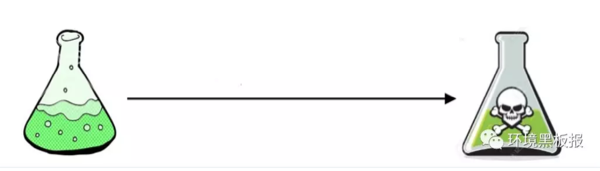
\includegraphics[width=8.33in]{images/dushui4}

\subsection{小结}

中国约50\%的水源受到微量有机化合物及重金属离子等物质的污染,令人堪忧的是,目前全国县以上4000多家自来水厂中,95\%以上仍然使用传统水处理工艺,这些工艺在处理有机化合物及重金属离子时,处理效果并不理想,同时,即使这些传统处理工艺能够在一定程度上去除该类污染物,更加有毒的转化产物也可能会生成使得自来水面临更高的健康风险,而普通民众对于这一事实却无处知晓。

水污染问题的确是个相当棘手的大问题,利益关系错综复杂,要完全改善也并非一朝一夕,是一个缓慢长远的过程!
笔者认为目前的水污染治理还存在诸多问题,首先,水质检测不够专业认真。几乎所有的饮用水专家和学者都认为中国的水质存在严重的安全隐患,但是在众多自来水厂的报告中,却几乎没有一家自来水厂自检水质不合格。这一看似矛盾的现象说明很多自来水厂在水质检测上并不认真,很多时候仅是马马虎虎测一些无关痛痒的参数告知民众自来水是安全的,但是背后真正的问题并没有被揭示出来。其次,污染控制不严,执法力度不够。自来水水质优,首先应得益于严格的水源控制。为保障水源安全,应建立水源保护区,在保护地带内,禁止一切有污染物质的进入,违者应被加以重罚。但我国目前的情况却是,许多工厂非法排污造成水源污染,但是当民众给所属环保部门报告时,监管部门大多并未作出积极的反应,或者即使作出反应,也仅是隔靴搔痒,并未真正杜绝该类地下排污问题的发生。

2015年``水十条''落地,预示着政府将握紧拳头向水污染宣战,笔者真心希望政府在以上问题上加大监管力度,对故意排污造成水污染的当事者予以重罚,同时对环保部门及水质检测部门加以规范,以期对水质状况获得最真实的第一手数据,为日后的水污染治理提供重要的观测基础。

作为与水息息相关的我们每一个人,除了等待政府可以更快更好的解决水污染问题,在日常用水中时要及时观察生活用水的水质变化,看其是否出现异常颜色或浑浊,有无异物及异味等。饮水前先放水,让水流一会儿,将管道中的``死水''流出再饮用。另外如有条件,建议增加具备反渗透膜过滤的净水器。

作者:李立平(博士,毕业于香港科技大学,从事水处理领域近7年,在相关研究领域发表学术论文数篇)
校稿:yufree,大石 编辑:丫头晚安

\section{一滴水的故事}

曾几何时,一滴水随着千万个同伴出现在这个星球。他们开始塑造这个星球,改变着地貌,孕育着生命。人类从出现的那一刻起,就开始了与水相爱相杀的历史。从两河流域的空中花园到尼罗河流域的金字塔,从马拉松的烽火到牧野之战的硝烟,水,孕育了地球最初的文明。同时,人类早先的传说,从诺亚方舟到大禹治水,又无处不在昭示着人类对水的敬畏。

水与人类的相爱相杀一直在进行着。有一滴水躲在茶壶里变成了蒸汽,告诉一位叫瓦特的人这样的力量可以推动机器运转,于是推动了轰轰烈烈的工业革命;有一滴水和同伴们一起构成了江、河、湖、海,让人类可以物流南北、货往东西,文明的火种得以靠水传播。

人类使用着水,也污染着水;净水养育着人类的同时,污水却时刻威胁着人类,这样的相爱想杀更是直接催生了我们的专业------环境科学与工程。此刻我们对水充满敬畏,毕竟水撑起了整个产业链上的勤劳的人们。水进入大气在不利的气象条件和污染物参与的情况下,形成雾霾,这一点我们在《混沌的冬日》里已经写过;水进入城市,若无法正常下渗、排除,则形成内涝,这直接催生了海绵城市的建设思路,这一点我们在《城市之殇》中已经展现;即使不听话的、因污染而变坏的水,工程师们不死心,坚信每一滴水都是清纯的,于是我们人类建立了污水处理厂,通过活性污泥法和生物膜法等工艺,使受污染的水改头换面,还清还纯,而这在《污师私房菜》中,我们也有所提及。

地球的水储量是巨大的,然而淡水资源却是如此的稀缺,环境工程师们在累死累活守护净水的同时,一个``开源''的灵感开启了水资源的另一段神奇之旅:

\subsection{海水淡化}

海水淡化方法主要分为热法和膜法。

热法:海水的盐度很高,直接饮用只会越喝越齁,但早在公元前1400年,海边的居民便学会了在锅内把海水加热到沸腾,使海水蒸发变成水蒸汽,盐分留在锅底成为垢,并使水蒸汽遇冷成为可饮用的蒸馏水。这也是今天常用的蒸馏法海水淡化的原型。而现代常用的热法海水淡化主要有多级闪蒸和低温多效两种。

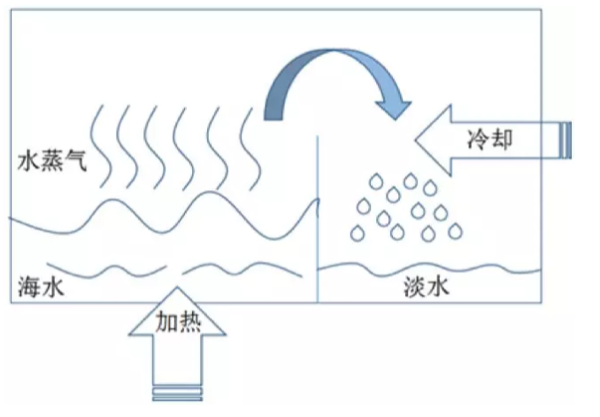
\includegraphics[width=8.33in]{images/seawater1}

膜法:1950年美国佛里达大学瑞德(C.E.Reid)教授在无意间发现了一个奇怪的现象。他观察到海鸥在海上飞行时从海面啜起一大口海水,隔了几秒后,吐出一小口海水,这个现象引起了他的思考。后来经研究发现,海鸥体内有一层薄膜,该薄膜非常精密,海水被海鸥吸入体内后,经过压力作用使水分子穿透薄膜转化为淡水,而含有杂质及高浓缩盐分的海水则吐出嘴外。于是,受此启发,瑞德教授提出了反渗透的基本理论。反渗透膜如同一只特殊的过滤筛子,在压力下过滤掉了水,而留下了盐(看到这里我觉得瑞德教授至少不是一个喜欢吃野味的人)。运用这一原理,我们就可以利用反渗透膜从盐水中获取淡水了。

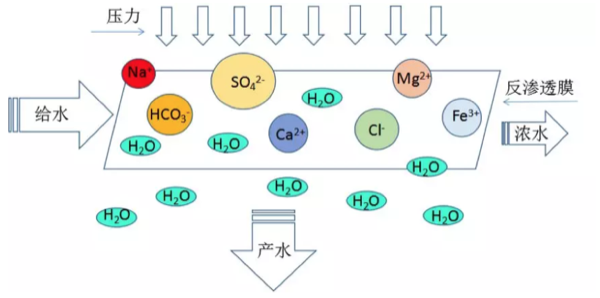
\includegraphics[width=8.33in]{images/seawater2}

我国人口占世界22\%,淡水占有量却仅为8\%,世界排序名列109位,是世界上12个严重贫水的国家之一。而海洋中蕴藏着丰富的淡水,其总量约占海水的97\%,相当于13.3亿立方公里之多,是一个巨大而又稳定的淡水储库。海水淡化作为水资源的开源增量技术,具有稳定供水、应急供水和战略性供水的特点,是解决沿海水资源短缺问题的重要途径。笔者收集了我国沿海地区人均水资源情况,发现沿海地区由于经济发展水平和人口密度较高,缺水情况反而高于全国平均水平,形成了靠水没水的情况。海水淡化成为了一些沿海地区解决缺水问题的关键手段之一。

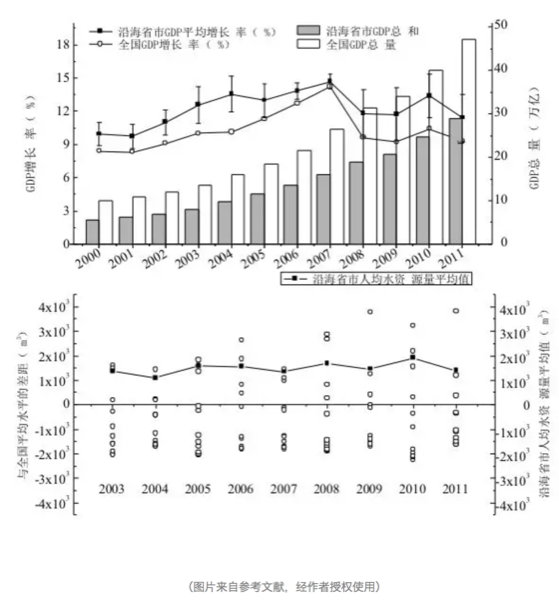
\includegraphics[width=7.76in]{images/seawater3}

我国海水淡化的历史始于上世纪五十年代。至2015年,全国总产能已经超过百万吨,约为全球海水淡化总产能的2\%左右。随着经济的发展,我国在国际海水淡化市场的比重逐渐增加。如下图所示,我国在这一年的产能增长约为中东地区的一半左右。中东地区存在一些自然条件上的限制,促使他们更加积极地开发海水淡化技术,因此中东地区历来是海水淡化最重要的市场,所以我们国家海水淡化产能比不过这些土豪真的不丢人。

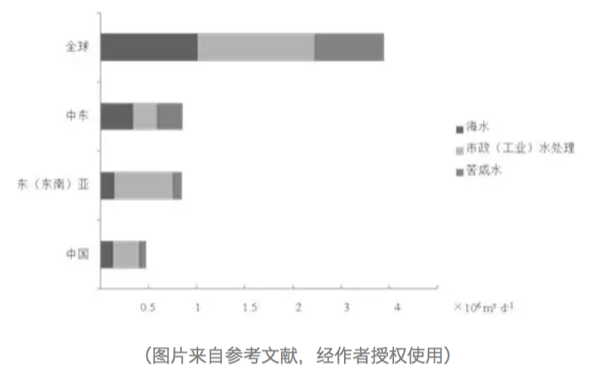
\includegraphics[width=8.33in]{images/seawater4}

目前我国已建的海水淡化产能主要集中在辽宁、天津、河北、山东等北方省市,这四省市产能占我国海水淡化总产能的81.9\%(2014年数据,见下表);与此对应的是不同省份对于海水淡化的关注度,下图是来自海水淡化的网络搜索指数,排行前五分别是北京、广州、浙江、江苏、山东,从中不难看出,海水淡化的关注度和接受水平也与地区的经济发展状况息息相关。

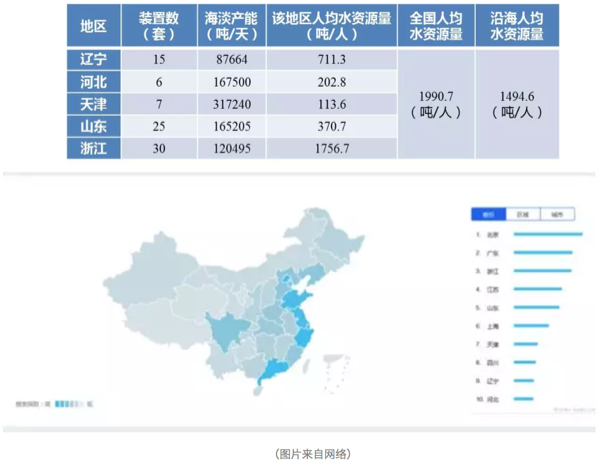
\includegraphics[width=8.33in]{images/seawater5}

2016年12月,国家发改委和国家海洋局联合印发的《全国海水利用``十三五''规划》指出,到``十三五''末,全国海水淡化总规模拟达到220
万吨/天以上,其中沿海城市新增海水淡化规模105
万吨/天以上,海岛地区新增海水淡化规模14
万吨/天以上。而海水直接利用规模拟达到1400
亿吨/年以上,海水循环冷却规模达到200
万吨/小时以上。新增苦咸水淡化规模达到100
万吨/日以上。海水淡化装备自主创新率达到80\%及以上,自主技术国内市场占有率达到70\%以上,国际市场占有率提升10\%。相信未来海水淡化会有更快的发展。海水淡化项目在某种程度上是一种基础建设项目,与各级政府的施政方向密不可分,所以虽然国家出台了一系列的规划政策,具体落地还是需要很长一段路。

\subsection{后记}

2010年,我们像一个一个水滴汇入了中科院这个汪洋大海,拥有了这片汪洋大海里的化学物质。随着时间的推移,我们又流到了其他地方,在各自的岗位上吸收了新的化学物质。不同物质间的反应总能产生新的物质,所以我们决定讲我们的源,讲述我们每一滴水的故事。

作者:yy 校稿:胜利屯支书,看透 编辑:栟 \#\# 小秸秆,大问题

2017年11月,演员孙艺洲拍戏途径哈尔滨,被郊县烧秸秆的烟熏味儿呛到流泪,随后在微博上抱怨:为什么一个白天空气质量优良的城市到了夜晚就空气爆表?为什么?怎么办?这个问题并不算新,但当它被一个拥有一千多万粉丝的耿直boy问出来的时候,还是结结实实触到了很多人的痛处。

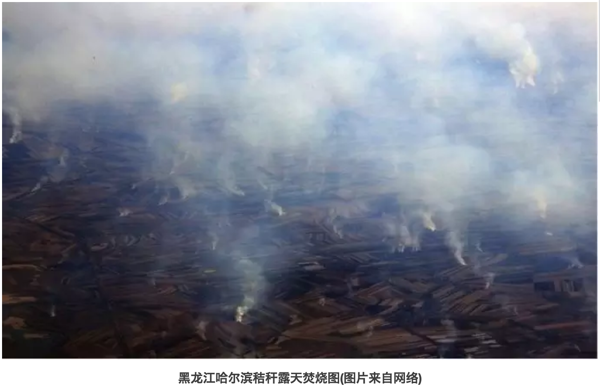
\includegraphics[width=8.33in]{images/stalk1}

在哈尔滨,把孙艺洲呛到流泪的是秸秆焚烧产生的颗粒物。每年秋收以后,庄稼被打捆、加工、再被送到每个人的餐桌上,算是完成了自己的历史使命;但秸秆这种副产品却被留了下来。

在田间地头,常常可见成垛的玉米或者小麦秸秆,勤快点儿的农户,将其垛得整整齐齐,也算是道风景;懒一些的,堆放得毫无章法,影响观瞻。

其实这个时候农民是真的忙。每年10-11月,是我国
``秋收秋种''期,各级农业部门一级战备、高度紧张,密切关注天气变化和降雨量,一轮又一轮的``紧急通知'',为的是指导农民收得时机合适,种得不早不晚。因为只有这样才能保证丰产丰收。

我们大东北黑土地在这个时候是收玉米种小麦,秋收整地追求``深、净、细、实'',小麦播种要在适宜播种期抢播早播。收下来的玉米秸秆无处可放,尽管我国80年代起就出台各种秸秆禁烧的相关规定,禁烧态势越压越重,但比起秸秆处理的经济压力和劳动力需求,很多农民不由自主就选择用``一把火''解决问题。

不烧不行啊,秸秆太多了。1991年我国秸秆产量为6亿多吨,经过了粮食总产量的``十三连丰'',到2015年,秸秆产量为10亿多吨。多出的秸秆总量为4亿多吨!什么概念呢?如果把这4亿多吨秸秆以100根为一扎首尾相连,能绕地球赤道转325000圈\ldots{}\ldots{}

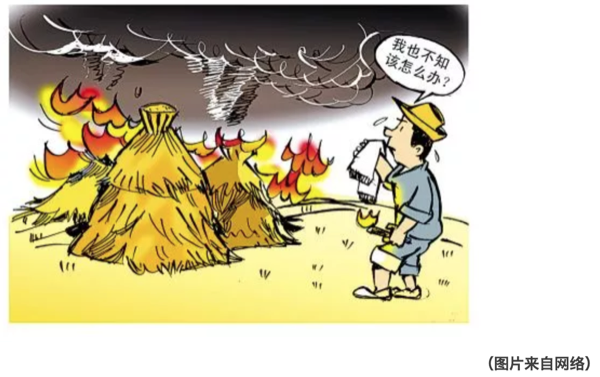
\includegraphics[width=8.33in]{images/stalk2}

不烧不行啊,农民家里实在没人。壮劳力都出去打工了,只剩下老人和孩子,尽管乡里承诺可以集中处理,那也需要把秸秆运输到集中处理点,老人孩子不会开车,没有工具,再好的政策也解不了眼前的急。

但烧秸秆的确是后患无穷。农作物光合作用的产物有一半以上保留在秸秆里,它富含氮、磷、钾、镁和有机质,秸秆大量集中燃烧的过程也是一种剧烈释放能量和物质的过程,周围环境根本无法在短期内消纳这么多的释放物,大气污染因此产生。

跟燃煤锅炉引起的污染不同,秸秆焚烧的主要产物是颗粒物、一氧化碳、二氧化碳等,对城市和乡村的低空空气影响更为直接。然而在大气污染研究领域,秸秆燃烧对雾霾的贡献一直颇有争议。

撇开具体贡献率不谈,稍加研究便可发现:在10月和11月的秋收期,从华北到东北(每年秸秆主要燃烧区),雾霾符合低硫份、高悬浮颗粒物、连片集中爆发的特点。

换句话说,叠加了大规模的秸秆焚烧,使得轻中度采暖季雾霾立刻升级为大范围重度雾霾。环保部10月期间的卫星遥感巡查监测数据分析表明,在16个省(区)共监测到疑似火点1583个,比2014年同期增长74.5\%,也的确证实了秸秆燃烧对雾霾的推波助澜``功效''。

所以,怎么办才好?秸秆问题和我国的大多数农业问题一样,工程浩大、解决起来困难重重。

目前秸秆的综合利用工作虽在稳步推进,但仍存在很大问题:一是秸秆还田成本高,运营公司与农户缺乏主动性;二是农民缺乏必要的技术支持,导致秸秆无法真正实现废物利用。

就东北地区来说,冬季气温偏低,秸秆还田要想充分被土壤消纳,必须使用进口农机深度翻耕,进一步增加了还田成本和土壤压力。说白了,东北地区黑土地耕作土层只有20厘米,想翻耕30厘米好让还田秸秆快速腐烂,需要钱,需要时间,需要人力,需要对新茬农作物减产的心理预期。

与这些困难形成对比的是,政府部门越来越强硬的禁烧手段。自1997年起,我国开始重视秸秆禁烧和综合利用工作,到2008年明确农作物秸秆综合利用分工、确定综合利用比例,再到2014年重拳出击京津冀及周边地区,提出部分地区全部实现秸秆综合利用的目标,禁烧力度越来越大。

进入2015年以后,我国出台了``史上最严''大气污染防治法,明确了县级人民政府应该补贴支持秸秆收储运和综合利用服务,并规定:露天焚烧秸秆的,可以处五百元以上二千元以下的罚款。

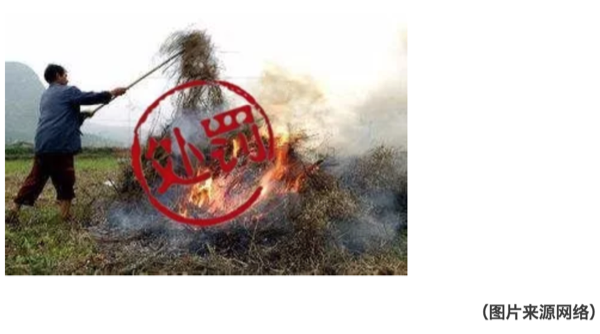
\includegraphics[width=8.33in]{images/stalk3}

为了彻底杜绝火点,在大气污染防治法的框架下,有些省份开出了自己的处罚清单。河南省在增加督查和暗访的基础上,以环保部公布的秸秆焚烧卫星监测火点数为依据,以县(市、区)为单位,出现一个火点,省财政扣拨县(市、区)财政资金50万元,力度之大空前绝后。

秸秆问题逐渐进入人们的视线并得到如此重视,除了它与雾霾之间千丝万缕的联系之外,还因为它的确是农业和环保领域牵一发而动全身的节点。

一根秸秆,一头连着三农,一个敏感脆弱又是万事之本的领域,一头连着环保,一个同样是成长痛点难点的行业。不能烧,但也不能接受粮食减产!粮食减产,根基没了,中国人民要挨饿;烧秸秆,污染加剧,人民叫苦连天。相信很多民生问题都是如此。

好在中国人民是世界上最勤快的人民。纵观其他国家,在面对这个问题的时候农民往往是两手一摊,对执法人员说``我没办法呀!''\ldots{}\ldots{}毫无悔改之意。

美国作为一个重要的粮食输出国,直到2011年在中部和东南部仍有大量火点发现,可比我国东北严重多了,有NASA图为证。印度人民更是开挂,烧着秸秆接受记者采访,大大方方毫不避讳。

秸秆的五料化利用技术(肥料化、饲料化、基料化、燃料化、原料化)并不高深,而秸秆问题的处理方式千差万别,对应效果天壤之别。

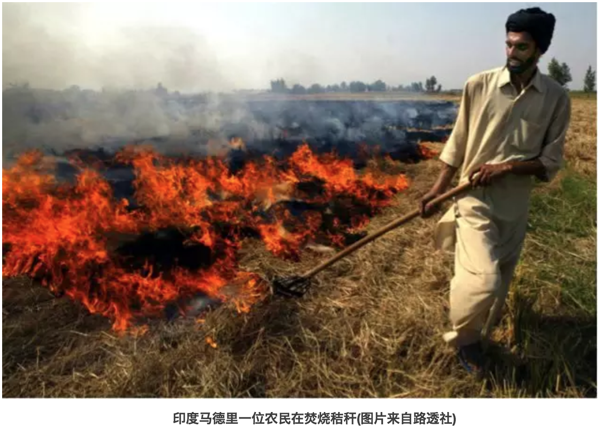
\includegraphics[width=8.33in]{images/stalk4}

解决秸秆问题,一个靠重视,一个靠财政。回看我国,重视程度和经济投入力度都需更进一步。

2007年,美国政府投资1.25亿美元建设了3个生物能源中心,专门进行纤维素生物能源研究。同年,美国农业部出资1400万美元、能源部出资400万美元,共同设立基金研发生物燃料、生物能源及相关产品的研究与开发。

据统计,2008-2012年,美国政府对生物质研发法中涉及的项目共计投资了1.18亿美元。除了对研发环节和支持外,美国对可再生能源发展规定了技术开发抵税和生产抵税的措施,生物质发电和秸秆纤维素乙醇项目都享受响应的税收补贴或者减免。

对比我国,2016年,农财两部门整合资金10亿元,选择秸秆焚烧问题较为突出的10个省份开展秸秆综合利用试点,取得了初步成效。果然真金见实效。

现在秸秆综合利用的主要方法是还田(直接和间接),直燃、气化、制沼,制醇和用作饲料、栽培基料等。

还田的方式简单、粗暴、直接、见效快,被各地采用最多,但由于地域差异明显,也存在一些弊端和后患。

直燃、气化、制沼和制醇等方式都需要大量的经费投入,各省由于财政状况难以统一,无法按照某个标准整体推进;另一方面,秸秆禁烧和综合利用与农户素质密切相关,在加大财政投入的同时,提高农民认识,增强回收利用秸秆的积极性也是较为有效的措施。

而在环境黑板报更新的《纳米非米》中,提出了以秸秆等有机废物为原料制备生物碳材料``以废制废''的观点,也是秸秆处理另一条可选择的路径。

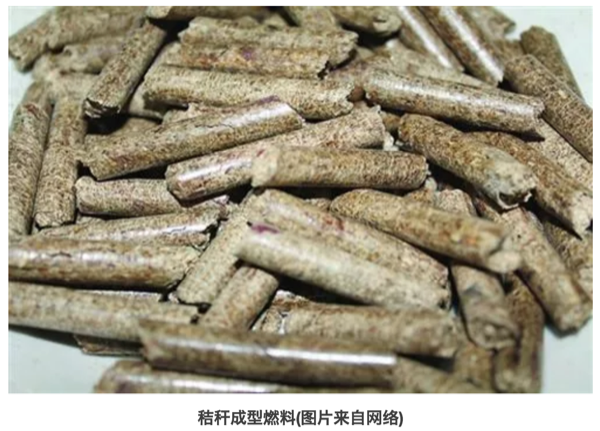
\includegraphics[width=8.33in]{images/stalk5}

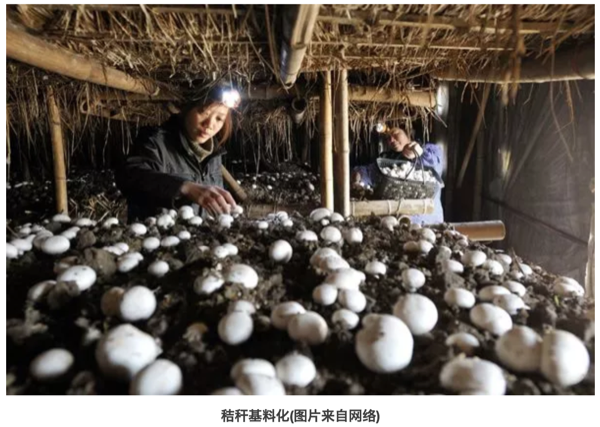
\includegraphics[width=8.33in]{images/stalk6}

\subsection{结语}\label{-1}

据悉,今年11月份哈尔滨火点问题爆出以后,相关责任人已于近日被环保部约谈,东北秸秆问题治理的机遇和挑战也随之而来。秸秆燃烧这种事,连遥感卫星都看得到,还怕执法部门不知道吗?小秸秆、大问题!希望所有的环保责任人能够直面问题,应对挑战。在关注大动向时,不忘记身边还有这样的``小事情''也同样需要我们的努力!

作者:胜利屯支书 校稿:广播站王站长、柴胡半夏苏 编辑:竹而乐 \#\#
VOC减排------大气治理的新挑战

\subsection{前言}\label{-1}

``今天空气质量怎么样?适不适合户外活动?''关注空气质量已经成了人们日常生活的一部分。由于人口增长和工业及经济的快速发展,人类在生活和生产中向大气中排放的污染物量也日渐增多,主要包括二氧化硫、氮氧化物、烟粉尘等颗粒物、挥发性有机化合物(Volatile
organic
compounds,VOCs)等等,而由此引发的大气污染问题也层出不穷:除了被热议的灰霾,酸雨、温室效应、光化学烟雾、臭氧层破坏、有毒物质扩散等也不容小觑。随着《大气污染防治行动计划》的实施,我国对二氧化硫、氮氧化物、烟粉尘排放控制取得明显进展,但VOCs防治工作相对滞后。目前,VOCs减排已经成为大气污染防治的重点。VOCs是什么?对于局外人来说,可能非常陌生,但在大气治理的圈子内,它已经火的不要不要了。那么,挥发性有机物到底是何方神物,会引起如此大的关注?

\subsection{VOCs是何物}\label{vocs}

\subsubsection{VOCs的定义}\label{vocs}

学术界对于VOCs的定义是指沸点在50\textasciitilde{}260℃,室温下饱和蒸汽压超过133.32Pa的易挥发性有机化合物。简单点说,挥发性有机物首先是有机物,然后这种有机物容易由液态转为气态物质进入环境空气中。举个例子,装修完之后,很多朋友会关心甲醛的问题。甲醛是胶粘剂的主要成分,板材中残留的和未参与反应的甲醛会逐渐向周围环境释放,甲醛就是生活中最常见的VOC。除了甲醛,生活中接触到的油漆、汽油等都含有VOCs。

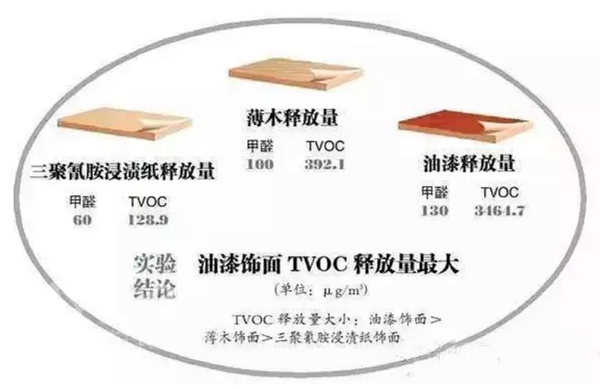
\includegraphics[width=8.33in]{images/voc1}

VOCs之所以被关注、被研究、被减排,就不得不说说它的危害。VOCs不仅危害环境,而且危害身体。一方面,VOCs是大气环境中光化学反应的前体,在阳光照射等特定条件下,会与环境空气中的化学物质,发生一系列光化学反应,生成臭氧,而形成光化学烟雾。同时,VOCs也是灰霾重要的前体物质,通过对细颗粒物(PM2.5)源解析,大气中VOCs在PM2.5中的比重占20\textasciitilde{}30\%,还有部分PM2.5由VOCs转化而来。

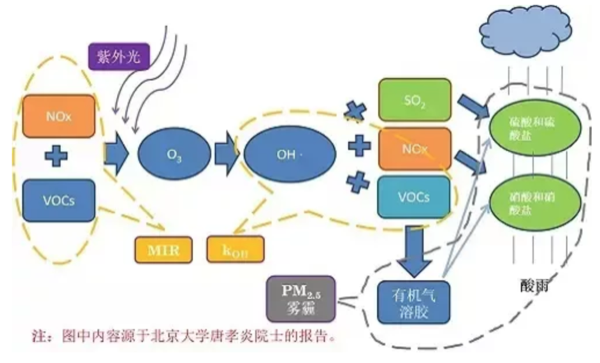
\includegraphics[width=8.33in]{images/voc2}

另一方面,大多数的挥发性有机物均有病理毒性,都对人体各器官组织有较大的危害作用。以甲醛为例,其在室内达到一定浓度,可引起眼红、眼痒、咽喉不适或疼痛等症状。

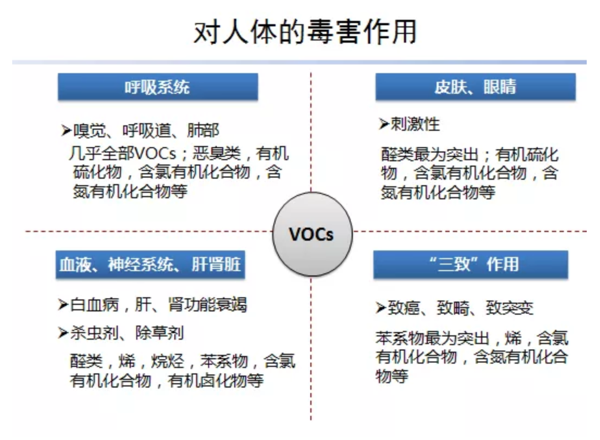
\includegraphics[width=8.33in]{images/voc3}

VOCs排放源主要包括自然源和人为源。自然源主要为植被排放、森林火灾、野生动物排放和湿地厌氧过程等,属自然界的正常规律,源和汇处于平衡状态。而人为源大致可分为工业源、生活源、农业源和移动源。有调查报道,我国VOCs的工业源和交通源为主要的人为源,分别占43\%和28\%。

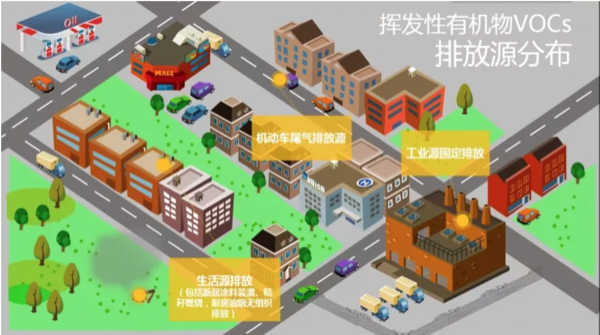
\includegraphics[width=8.33in]{images/voc4}

其中工业源排放企业涉及的行业有电子信息、纺织印染、石油化工、家具、木材加工、塑料橡胶制品加工、包装印刷、制药等,这些行业也正是目前我国主流工业。正因为人类活动,越来越多的VOCs进入大气中,在环境空气中的累积,打破了自然界VOCs源和汇的平衡。

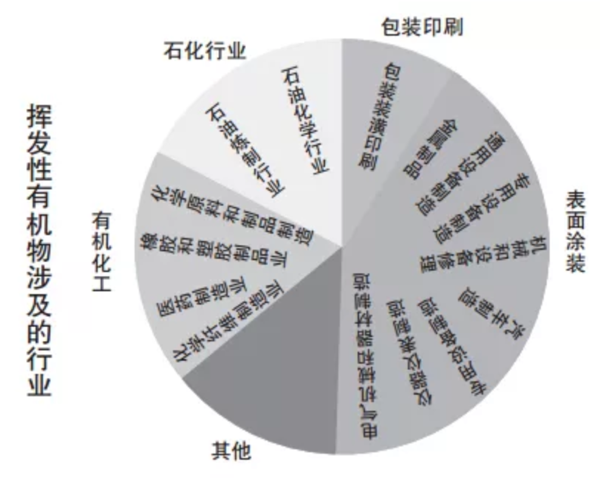
\includegraphics[width=8.33in]{images/voc5}

1940年至1960年间,美国洛杉矶多次发生光化学烟雾事件。在1952年12月的一次光化学烟雾事件中,洛杉矶市65岁以上的老人死亡400多人。1955年9月,由于大气污染和高温,短短两天之内,65岁以上的老人又死亡400余人,许多人出现眼睛痛、头痛、呼吸困难等症状甚至死亡。事件的主要原因是汽车尾气排放了大量的碳氢化合物,在阳光照射下,发生光化学反应,产生有毒气体。这是人类首次认识到VOCs的严重危害,因此,洛杉矶对VOCs的关注走在了世界的前列。1963年,美国以《清洁空气法》的规定为基本依据,要求卫生教育福利部处理空气污染问题,明确机动车对空气污染的影响,并通过环境保护署制定和颁布限值VOCs污染排放的一系列标准,指导全国执行VOCs排放限值。1970年7月,日本东京出现了光化学烟雾现象,几所大学连续出现学生眼睛疼痛、呕吐等现象。因此,日本在VOCs污染排放方面的关注也比较早。

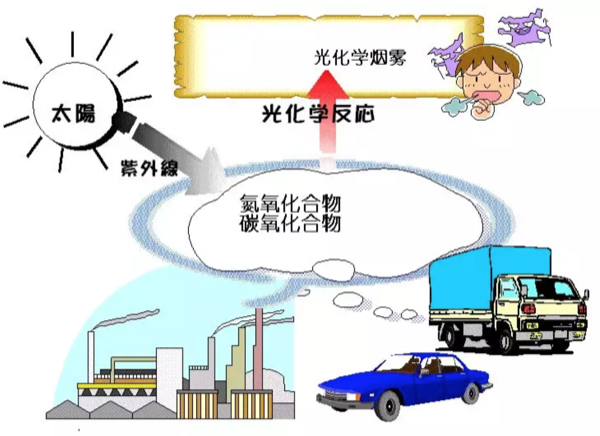
\includegraphics[width=8.33in]{images/voc6}

\subsection{VOCs的减排之路}\label{vocs}

\subsubsection{国家层面}

我国尚未出现过VOCs污染事件,因此对其关注较晚,2000年,《中华人民共和国大气污染防治法》中仅有诸如有机烃类尾气、恶臭气体、有毒有害气体、油烟等类似概念。

随着灰霾问题的深入研究和环境空气中臭氧浓度升高问题,VOCs逐渐被重视。为改善大气环境质量,促进VOCs削减,我国出台了一系列的政策。2013年,国务院出台《大气污染防治行动计划》,明确要对石化、有机化工、表面涂装、包装印刷等行业实施VOCs综合整治,全国范围内的VOCs减排正式启动。同年,环境保护部编制了《挥发性有机物(VOCs)污染防治技术政策》,为VOCs减排提供了技术规范支持。2015年8月29日第十二届全国人大常委会第十六次会议通过了《中华人民共和国大气污染防治法》,自2000年修订以来,首次增加对VOCs控制要求,从此VOCs减排有了法律依据。这些政策的颁布,从计划到技术、再到立法,逐渐指明我国VOCs减排方向。

在部门规章方面,国家发改委、环保部、财政部、工信部、质检总局、能源局等部委相继出台了有针对性的VOCs污染防治相关文件。各部门相互配合,共同打好VOCs减排攻坚战。

在技术标准方面,我国《大气污染物综合排放标准》(GB162972-1996)对14类VOCs规定了最高允许排放浓度、最高允许排放速率和无组织排放限值,其中包括甲醛、苯、甲苯、二甲苯等挥发性有机物。针对不同的有机污染物排放源以及污染源和环境空气中VOCs的监测技术,截止到2017年,环保部总共制订了15个涉及VOCs的排放标准和20个监测技术方法。从标准实施年限来看,2010年以前,只有3个排放标准和8个监测技术方法,其他都是近几年开始实施。技术标准的制定,为VOCs减排提供了监测和排放依据。

\subsubsection{地方层面}

为积极推动VOCs减排,各地结合地方实际,出台了一系列相关的政策法规和标准方法。表
1列举了北京和江苏省的VOCs污染防治政策。由表
1可见,我国地方从2010年前后,开始加强对VOCs进行管控。近一两年,VOCs污染防治成为各地大气防治的重点工作,各地不断完善VOCs减排政策措施。

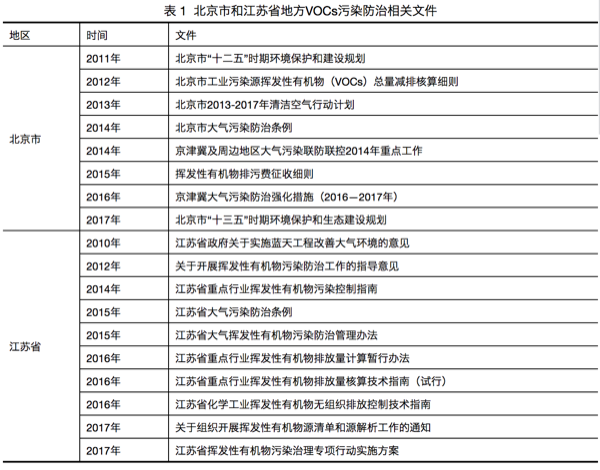
\includegraphics[width=8.33in]{images/voc7}

在技术标准方面,国内出台VOCs排放标准的省市并不多,以北京、江苏、浙江和广东为例,各地根据当地的产业特点,制定了相关VOCs排放标准。近两三年,北京连续制定了12项地方排放标准,涉及的行业有印刷、家具制造、炼油和石油化工、汽车、工业涂装和建筑涂料等;江苏重点针对化学工业和表面涂装行业,制定了相关地方排放标准;浙江以化学合成制药、制鞋、化学涂装、纺织染整行业为重点行业;广东以集装箱制造和电子行业为重点行业。

\subsection{VOCs减排技术和挑战}\label{vocs}

对VOCs减排的主要技术思路是源头控制和末端治理。简单的说,源头控制就是从原料开始,减少VOCs的产生。末端治理,顾名思义,将产生的VOCs进行最终的销毁。有两类基本技术,一类是回收技术,对排放的VOCs进行提纯处理,再资源化循环利用。主要包括吸收、吸附、冷凝和膜分离方法等技术。另一类是销毁技术,将排放的VOCs分解化合转化为其他无毒无害的物质。主要包括活性炭吸附、低温等离子、热力燃烧、催化燃烧等技术。

涉及VOCs排放的行业众多,污染物种类繁多,废气成分复杂,因此,在对VOCs减排时,要考虑技术上有效、经济上可行,往往这两者很难平衡,这也是VOCs减排面临的最大的挑战。

\subsection{小结}\label{-1}

因此,虽然我国对VOCs的管控起步较晚,为改善环境空气质量,近年来,我国已将VOCs减排作为一项重点工作,出台了相应的法律、法规、政策、技术规范等,并迅速形成一套体系,为VOCs污染防控指明了方向,提供了支撑和保障。

``大家非常关心中国会不会发生光化学烟雾事件,中国政府也高度关注。我们组织过专家分析,世界历史上发达国家发生的光化学烟雾一般臭氧浓度都达到了600以上,个别城市2000以上。中国的臭氧浓度远低于此,所以中国现在和将来不会、也极少可能会发生光化学烟雾事件。''引用环保部大气环境管理司司长刘炳江的一段话,作为总结,相信我国VOCs减排之路,对环境改善有重要的意义。

作者:远方老友 校稿:广播站王站长、柴胡半夏苏 编辑:栟

\section{生态•五行•人伦}

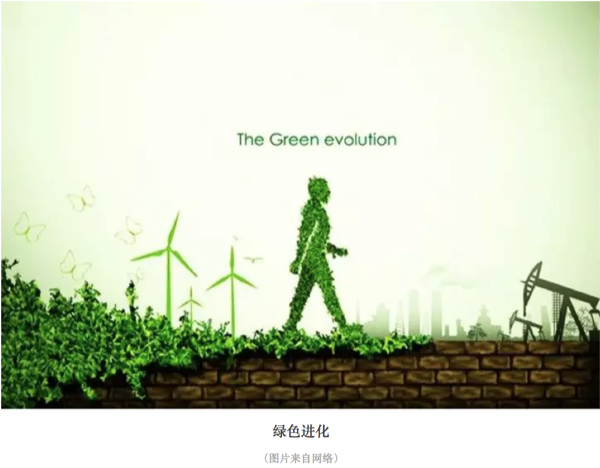
\includegraphics[width=8.33in]{images/swr1}

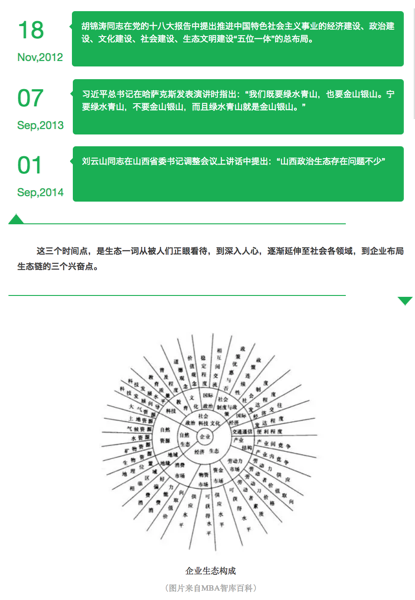
\includegraphics[width=5.76in]{images/swr2}

往事有时令人不忍直视。想当初,环境保护也曾贵为与计划生育相互比肩的两项基本国策之一。然而,一直以来,世人只知后者威加海内,却与前者对面不识。三十年河东,三十年河西。现如今,环境保护俨然已成尚方宝剑,坐拥一票否决权,何止扬眉吐气,大快人心。人们对生态环境保护的关注前所未有。本文也顺着风向,用陈词旧调来赶一次时髦。

一般来说,人们生活的环境通常分为自然环境和社会环境。自然是天与地,天与地之间的万物按照``道''的规律循环不息的现象和状态,包括人类和其他生命世界、物质世界的一切活动。生态是指生物在一定的自然环境下生存和发展的状态。我们人类研究生态,也就是要研究怎样保护和利用自然环境以服务人类的发展,也就是要弄清楚自然是怎样在影响着人类的活动。

研究生态的原理和方法很多,无论东方和西方,还是古代和当代,都有自成体系的表达。本文主要介绍一下在中国古代的五行理论中环境是怎样影响人的。

150年前,马克思提出:``运动着的物质世界是普遍联系和永恒发展的'';3000年前,五行系统理论把这些运动、联系和发展以取象的方法做出了精致的总结。

在五行理论中,根据运动和显现的方式将事物分为木火土金水五类。五行包括气(炁)和象,属于同类五行的事物相互感应。所谓的``天人合一''、``天人相感'',在这个角度讲就是天、地、人、万物之间是一体的,是一直在相互感应的。

为了问题聚焦,我们在这里不具体讨论感应的媒介是电波、磁场,还是量子纠缠,只强调说当某一类五行出现问题的时候,属于这一类五行的所有事物都会受影响。也就是说天地间某一类五行的气(炁)出现问题了,那么赖以这一类五行的气(炁)所支撑的象必然也就要出现问题。我们也不在这里科普具体的五行系统理论,只是应用五行的理论来探讨生态与人伦的问题。这里的人伦包括人的社会伦理和家庭伦理。

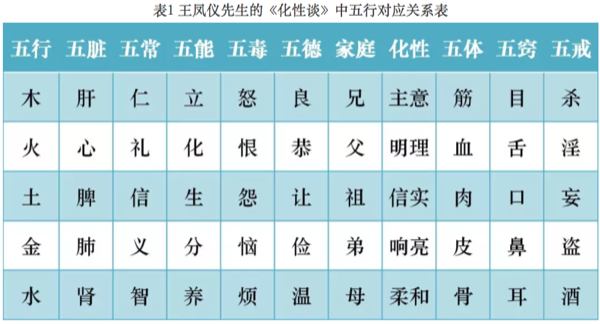
\includegraphics[width=8.33in]{images/swr3}

限于篇幅,此次只简单讲一个离我们最亲近的五行:大地母亲------土五行。

当前,土壤中重金属超标、农田里化肥农药高残留等问题,导致土地受到了普遍破坏。因为破坏的规模和程度足够大,引起了``土''五行气(炁)和象的破坏。

土对应信。所以,当前社会诚信普遍缺失。具体表现为:人们说过的话容易变卦,谈好的事兑现不了(谈十个事情甚至成不了一个),签过的协议无法履行,约定的日期时间不能遵守,制售贩假货泛滥。这里的真实情况不一定是人们主动的不讲诚信,有很大部分是环境在对事件本身产生影响。

土对应怨、脾胃、祖辈、口、安全感。土德受损,人们遇到问题容易怨天尤人,脾胃功能不好,与祖辈少有连接和沟通(包括祭祖),容易打妄语(恶口、两舌、绮语、诳语),贪吃、什么都吃而且吃不到什么好东西。人们普遍缺乏安全感。

土地肥沃、平坦、无污染的地区,人们则是讲信用、不怨人(心胸开阔)、与祖辈亲近(老人容易有儿孙绕膝的天伦之乐)、饮食有节制、不妄语、脾胃好,有安全感。

当土地出了问题,其生长出来的食物自然就要受影响,导致人吃了之后也就有问题。土地贫瘠,土壤中某些元素过剩、毒素残留,会导致食物营养成分不全或者有毒素,人吃了之后自然就会在心理和行为上有相应的表现。吃水培(无土栽培)食物也是如此。长期如此,整个社会也就出现变化。

土地缺失或者供应不足,土地状态被破坏,都会对当地的人和社会状态产生相应影响。

另一方面,一方水土养一方人。医院里的营养师都知道,北方人需要补充维生素的话要吃苹果,而吃香蕉的效果就不如苹果理想。但陕西的苹果的营养对陕西人最适用,本地人最适应本地的农作物。转基因的农作物结出的果实因为无法再当作种子进行发芽生根,所以人吃了会影响生育。

脾属土,主肌肉。人是父精母血交媾而成,从父亲那得了骨,从母亲那得了肉。断奶之后,我们靠土地长出的食物来长肌肉。断奶前应该食母乳。现在人们都是给孩子喂牛奶。而牛奶适合牛的胃,适合牛的营养需求。当前婴儿普遍吃母乳不足,容易导致肌肉和脾胃系统出现问题,长大与母亲不太亲近,也会影响孩子土五行的运转和土德的圆满。

土五行就是这样影响着人与自我的和谐、与家庭的和谐、与社会的和谐。有一个好的生态系统,首先是有好的土地,因为土地不仅是五行之一,还担当着万物的生化、收纳和承载。

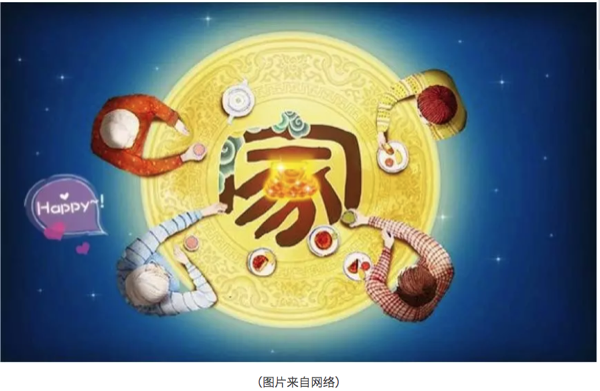
\includegraphics[width=8.33in]{images/swr4}

作者:含章 编辑:栟

\section{油田环保之痛------含油污泥}

\subsection{序:油田环保的痛处}

石油作为一种重要的资源,在国民经济发展中具有支柱性地位,不仅支持着工业农业生产,也与每个人的生活息息相关。2011年至2015年间,我国每年的石油开采量持续高于2亿吨。

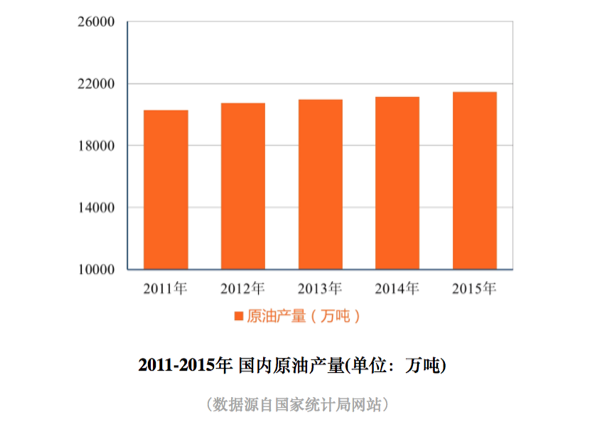
\includegraphics[width=8.33in]{images/youni1}

石油资源开发与使用过程中造成的污染是令全世界头痛的一大难题。举世震惊的墨西哥湾漏油事件,造成了严重的生态灾难,令难以计数的生物遭遇灭顶之灾,沿岸生态遭遇了极大破坏,也使得石油生产过程中的环保问题引起了大众的关注。事实上,在石油业的生产过程中,除了事故导致原油泄露造成的直接环境污染外,在石油开采和加工过程中产生的含油污泥也是一个重要的污染源,且会对周边生态环境造成持续性的危害。

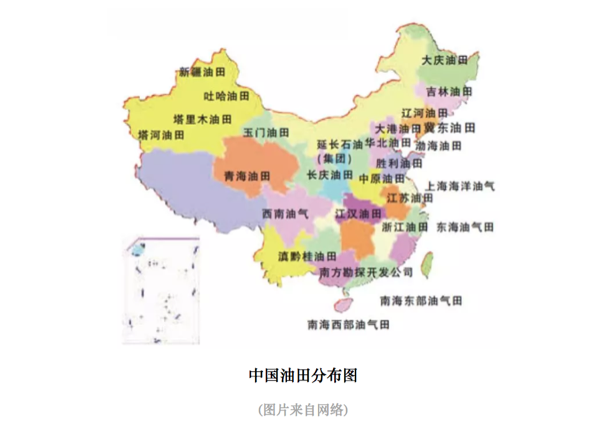
\includegraphics[width=8.33in]{images/youni2}

\subsection{含油污泥的来源}

含油污泥,简称油泥,是在石油开采、运输、炼制及含油污水处理过程中产生的含油固体废物,是由石油烃类、胶质、沥青质、泥砂、无机絮体、有机絮体以及水和其它有机物、无机物牢固粘结在一起的乳化体系。

含油污泥主要产生在油田和炼油厂,分为3
种类型,即落地油泥、集输油泥和炼厂油泥。落地油泥是在油田开发特别是油井采油生产和井下作业施工过程中,部分原油放喷或被油管、抽油杆、泵及其他井下工具携带至地面,进而渗入地面土壤形成的油泥;集输油泥是储油罐在自然沉降中产生一些油泥,也称之为称为罐底泥;炼厂油泥主要细分有三种,分别为隔油池底泥、溶气浮选浮渣和剩余活性污泥等,其中以浮选浮渣量为最大,占三泥总量的80\%。

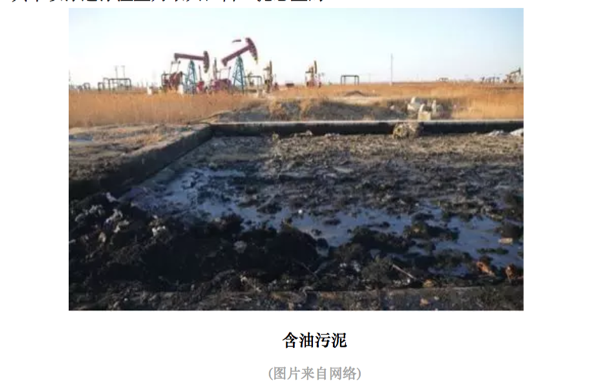
\includegraphics[width=8.33in]{images/youni3}

目前,我国每年产生近百万吨的含油污泥,若加上石油化工产生的``三泥''(生化污泥、池底污泥及浮渣),油泥的总量还要大得多,而且炼厂的规模越大,含油污泥的排放量越大。

\subsection{含油污泥的成分与特性}

含油污泥成分非常复杂,含有大量的老化原油,固体悬浮物,以及细菌质等固体废物,其中原油是主要的成分。油泥中含有数百种有毒有害化合物,其中的某些化合物(多环芳烃等)具有``三致''效应;另外含油污泥中往往含有苯系物、酚类等物质。美国环保署(EPA)将其列为优先污染物,并且对其排放有严格的限制,我国也将油泥列入《国家危险废物名录》。

含油污泥的特性:一般含油污泥的含油率约10\%-50\%,含水率约40\%-90\%。黏度高,难以沉降,脱水效果差,污泥固相颗粒细小,油、水密度差小,这些都是含油污泥黏度大、难以除油脱水的主要原因。

\subsection{含油污泥的危害}

含油污泥因其体积庞大,并含有大量的有毒物质,直接进行排放会占用大面积的土地,同时伴有非常难闻的气味,对附近的土壤、植物、水体、空气造成严重的污染,最终对人体产生极大的危害。

\begin{itemize}
\tightlist
\item
  影响土壤的性质
\end{itemize}

当含油污泥中的石油烃类等物质渗入土壤后,会在土壤颗粒表面黏着,直接影响土壤的通透性,从而造成土壤导水通路的阻塞,进而造成土壤渗水量的下降,透水性的降低,最终使土壤的性质发生改变,直接威胁到土壤中的微生物生存。

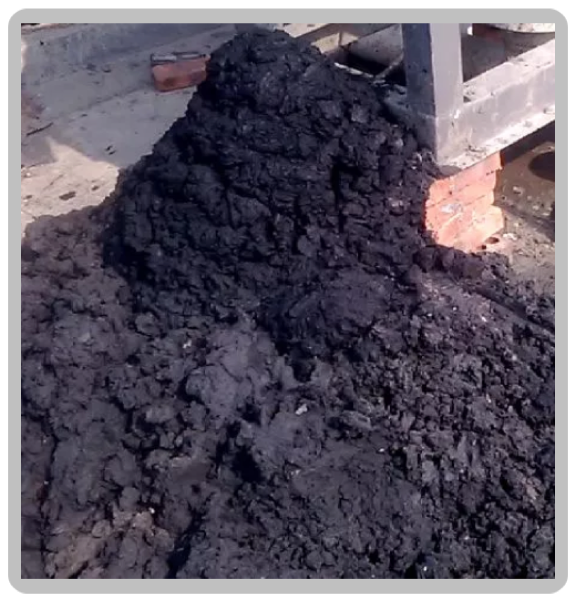
\includegraphics[width=8in]{images/youni4}

\begin{itemize}
\tightlist
\item
  危害植物生长发育
\end{itemize}

植物的组织内部能够被含油污泥中的低分子烃类物质渗透,从而破坏植物的正常生理机制;而含油污泥中的高分子烃类会很容易在植株表面形成一层粘性膜,将直接阻塞植株的气孔,植株的水吸收作用以及呼吸和光合作用都会受到严重的影响,最终会造成植物根系的腐烂,植被的破坏将会引起生态系统中食物链的破裂,会导致生态系统中最初级生产者失去制造有机物和氧气的能力。

\includegraphics[width=8.33in]{images/youni5}

\begin{itemize}
\tightlist
\item
  污染水体
\end{itemize}

含油污泥中的石油类污染物浸入地下水后,直接对饮用水资源和地下水资源造成影响,危及人类生命安全。另外,含油污泥处置不当,可能会使石油类污染物在水体中聚集,如码头、港口、河道沿岸等,破坏水体环境。

\includegraphics[width=8.33in]{images/youni6}

\begin{itemize}
\tightlist
\item
  危害空气质量
\end{itemize}

含油污泥中的低沸点有机污染物极易挥发至空气中,有机硫化物、苯类、酚类等有害物质具有致癌、致畸、致突变的作用,随着呼吸进入人体,直接对人体的肺、胃、呼吸系统、神经中枢系统产生严重的危害。

\includegraphics[width=8.33in]{images/youni7}

\subsection{相关控制标准}

在国家层面,目前与含油污泥相关的控制标准有《危险废物填埋污染控制标准》(GB18598---2001)、《危险废物焚烧污染控制标准》(GB18484---2001)、《农用污泥中污染物控制标准》(GB4284---84)。在《危险废物填埋污染控制标准》和《危险废物焚烧污染控制标准》标准中,将含油污泥归类为危险固体废物,但并没有对含油污泥的油含量提出量化指标。在《农用污泥中污染物控制标准》中,对污泥中的矿物油含量做了明确规定,要求土壤中矿物油最高允许含量不得超过3000
mg/kg(≤0.3%)。地方层面主要有以下三省份制定了相关标准:2010年12月,黑龙江省发布了《油田含油污泥综合利用污染控制标准》,明确规定了含油污泥用于农用、铺设油田井场和通井路的污染物控制标准;2016年7月,陕西发布《含油污泥处置利用控制限值》,规范含油污泥回收利用处置;2017年6月,新疆维吾尔自治区发布《油气田含油污泥综合利用污染控制要求》。

\includegraphics[width=8.33in]{images/youni8}

\subsection{含油污泥的处理处置}

如果含油污泥得不到妥善处理,将造成资源的巨大浪费,同时也会对环境造成不可挽救的破坏。因此,采用合适的处理方法对含油污泥进行资源化与无害化处理,不仅可以减少环境污染,而且还能达到资源再利用的目的。当前的油泥处理技术主要包括热解法、调质离心分离、固化处理、焚烧、焦化、填埋、溶剂萃取、热碱水洗、电化学技术、生物处理
(包括地耕法、堆肥法、污泥微生物反应器法)等。

由于含油污泥来源广泛、成分复杂,同时处理技术种类繁多,且都存在各自的应用弊端和适用范围(不同技术的特点比较如下表),目前尚无任何一种技术可以作为处理所有类型含油污泥的理想方法。通常要根据油泥的来源及特性,有针对性地选择一种或者多种组合技术实现油泥的治理。

\includegraphics[width=8.33in]{images/youni9}

\subsection{处理存在的难点和技术展望}

随着新环保法的通过,各地对油田环保的要求越来越高,含油污泥的随意排放将不再可能,各地隐藏的污染也被逐渐揭开。这对污泥处理行业来说,无疑发展前景利好。尽管油泥处置发展前景好,市场也很大,但是目前含油污泥处置也存在一些难点,同时对其发展前景进行梳理如下:

\begin{itemize}
\item
  含油污泥中最难处理的是重质油油泥,其黏度大,沥青质及胶质含量高,回收难,在现有的工艺设备处理过程中成本较高,设备折旧快,因此降黏预处理是此类油泥处置的重要环节;
\item
  热解方法由于是在厌氧环境条件下热源对含油污泥间接加热,能够通过油气组分的挥发分离实现油泥中石油组分的回收,同时降低残渣中的含油率,是一种油泥无害化与资源化的综合处理工艺。因此,该技术是近三年来油泥处置行业极为推崇的热点实用工艺,尤其在能源价格低、油泥组分中砂质组分含量的西北地区的油泥,更适合推广该技术;
\item
  热解方法尽管处理含油污泥非常实用有效,但是与调质离心等减量化工艺相比,仍存在耗能高、处理规模小等问题,因此,在以后的研究过程中亟待开发提高热解处理效果与规模的带有新型热源的新一代热解设备;
\item
  微生物及植物修复方法尽管修复周期长,却非常适合低浓度石油污染的场地及油泥处理,是物理与化学方法后续深度处理含油污泥的重要补充措施。为了使植物修复最终成为解决实际环境问题的有效手段,如何将石油污染的植物修复从盆栽实验的研究成功转向田间试验及实际的工程尚需进一步的深入研究;
\item
  目前含油污泥高级氧化技术在东北及西北地区油田的油泥处理工程中得到有效的实际应用,但该方法存在药剂成本高、处理的油泥残留化学药剂等问题,因此开发环境友好、氧化能力突出的绿色修复药剂就显得尤为重要;
\item
  目前油泥处理的验收标准往往是以含油率为重要指标,但是缺乏具体的石油烃组分的定性定量分析,鉴于不同组分的生物有效性及环境风险有很大差异,因此在以后的研究中有必要深度细化处理后含油污泥的石油组分含量,进一步明确验收标准。
\end{itemize}

作者:OILs 校稿:周宁、爱杯子的王小咖 编辑:栟

\section{\texorpdfstring{斯德哥尔摩公约和它``锁''住的POPs}{斯德哥尔摩公约和它锁住的POPs}}\label{pops}

\subsection{管控持久性有机污染物的斯德哥尔摩公约}

随着国家层面对环保的重视,公众也越来越多的开始关注环境污染问题。大家可能时常听到一个词------POPs,一个读起来略带喜感的单词缩写,但它指代的物质却十分``恐怖''。POPs是持久性有机污染物(Persistent
Organic
Pollutants)的简称,是指那些具有生物蓄积性、能够通过各种环境介质长距离迁移并长期存在于环境中,对人类健康和生态环境造成严重危害的天然或人工合成的有机化合物,其污染的复杂性远超过常规污染物。一些POPs具有三致效应(致畸、致癌、致突变),它们的危害往往具有隐蔽性和突发性的特点,一旦发生重大污染事件,将产生灾难性后果并持续危害几代人。例如1968年3月发生在日本的米糠油事件,由于管理不善,致使生产米糠油时混入多氯联苯,产品被人食用后导致中毒,患病者超过5000人,30余人死亡,实际受害者约13000人。症状主要表现为咳嗽不止,肝功能下降,全身肌肉疼痛,重者发生急性肝坏死、肝昏迷等,及至死亡。副产品之一的黑油作为饲料喂养家禽后造成数十万只家禽死亡。这是一起典型的POPs中毒事件,当时震惊了全世界。

为此,2001年联合国环境规划署通过了旨在控制POPs的《斯德哥尔摩公约》(下文简称公约),作为保护生态环境和人类健康免受有机污染物危害的全球行动。目前,已有包括我国在内的179个国家和地区加入了公约,从缔约国数量上可以看出公约的国际影响力,同时也能看出各个国家对于POPs污染的重视。其中公约规定的12种POPs,即氯丹、艾氏剂、狄氏剂、异狄氏剂和七氯、滴滴涕、六氯苯、多氯联苯、毒杀芬、灭蚁灵、多氯二苯并呋喃、多氯二苯并-对-二恶英等,被称为``肮脏的一打(dirty
dozen)'',受到缔约国的严格控制与削减。在国际公约的推动下,国际上有关POPs的相关研究也逐步深入,已成为环境科学研究中最受关注的热点领域之一(见图1)。

\includegraphics[width=8.33in]{images/gongyue1}

随着人类经济活动的快速发展,许多新型POPs,如氯化石蜡、全氟化合物、溴代阻燃剂等也不断在各种环境介质中被发现,逐渐成为关注的焦点。这些物质绝大多数是正在大量生产和使用的化工产品,目前尚未对其生产排放进行有效管控,而且相关的人体健康风险、生态风险和毒理学数据还较为缺乏,难以准确评估其生态和健康效应。

\includegraphics[width=8.33in]{images/gongyue2}

公约如何将某种POPs列入管控对象呢?公约规定了任一缔约国均可向秘书处提交旨在将某一化学品(拟增列POPs)列入公约附件的提案。而公约秘书处将提案转交给持久性有机污染物审查委员会(POPRC)后,将依次审查其是否符合公约附件D(化学品的持久性、生物富集性、长距离迁移能力及不利影响),附件E(评价该化学品是否会因其远距离迁移而对人体健康和/或环境产生重大不利影响)和附件F(涉及社会经济考虑因素的信息)对POPs的要求,如果全部符合,POPRC会根据风险管理评价的结果提议是否由缔约国大会审议该化学品以便将其列入附件并规定相应的管控措施(流程见图3)。

2009年5月,在瑞士日内瓦举行的缔约方大会第四届会议决定将全氟辛烷磺酸及其盐类、全氟辛基磺酰氟、四溴联苯醚、五溴联苯醚、六溴联苯醚、七溴联苯醚、十氯酮、六溴联苯、林丹、五氯苯、α-六六六、β-六六六等新增化学物质列入公约附件的受控范围。2011至2015年间的缔约方第五次会议、第六次会议以及第七次会议又分别决定将硫丹及硫丹硫酸盐、六溴环十二烷、多氯萘、六氯丁二烯和五氯苯酚等物质增列到公约POPs名单。2017年5月第八次会议将十溴联苯醚、短链氯化石蜡以及六氯丁二烯正式增列为公约POPs候选名单。目前正在进行审查的物质包括三氯杀螨醇、全氟辛酸及其相关物质。

\includegraphics[width=8.33in]{images/gongyue3}

\subsection{POPs的持久性}\label{pops}

``环境持久性''是POPs最主要的特点之一,是界定一种物质是否为POPs以及筛选新型POPs的重要判据,也是评价有机污染物对环境和人类潜在危害的基础以及开展化学品风险评估的关键依据。公约附录D关于持久性的评价标准为:对于通过空气大量迁移的化学品,其在空气中的半衰期应大于两天、或者该化学品在水中的半衰期大于两个月、或在土壤/沉积物中的半衰期大于六个月;或该化学品具有其他足够持久性、因而足以有理由考虑将之列入本公约适用范围的证据。

\includegraphics[width=8.33in]{images/gongyue4}

\subsection{POPs的生物富集性/放大性}\label{pops}

生物富集和放大性是指化学物质可被生物组织吸收,并在生物体内持续累积,而且这些物质的浓度会沿着食物链/网传递(图5),随着营养级升高呈现放大趋势,在高等生物体内出现高浓度,影响高等生物的健康。公约对POPs的生物富集性/放大性的规定为:(1)表明该化学品在水生物种中的生物浓缩系数或生物富集系数大于5000,或如无生物浓缩系数和生物富集系数的数据,但有logKow大于5的证据;(2)表明该化学品有令人关注的其他原因的证据,例如在其他生物中的生物富集系数较高,或具有高度的毒性或生态毒性;(3)生物监测数据显示,该化学品所具有的生物富集潜力足以有理由考虑将其列入本公约的适用范围。

\includegraphics[width=8.33in]{images/gongyue5}

\subsection{POPs的长距离迁移能力}\label{pops}

POPs具有长距离迁移特性,以大气和水体为载体,通过``高山冷捕集效应''和``全球蒸馏效应''到达高海拔的偏远高山地区和高纬度的极地地区,从而导致全球范围的污染。公约对远距离环境迁移的评判标准如下:

(1)在远离其排放源的地点测得的该化学品的浓度可能会引起关注;

\begin{enumerate}
\def\labelenumi{(\arabic{enumi})}
\setcounter{enumi}{1}
\tightlist
\item
  监测数据显示,该化学品具有向环境受体转移的潜力,且可能已通过空气、水或迁徙物种进行了远距离环境迁移;
\end{enumerate}

(3)环境转归特性和/或模型结果显示,该化学品具有通过空气、水或迁徙物种进行远距离环境迁移的潜力,以及转移到远离物质排放源地点的某一环境受体的潜力。

\includegraphics[width=8.33in]{images/gongyue6}

\subsection{中国的实施计划}

我国政府于2001年5月23日签署了《关于持久性有机污染物的斯德哥尔摩公约》,2004年6月25日第十届全国人大常委会第十次会议做出了批准《斯德哥尔摩公约》的决定。公约于2004年11月11日对中国正式生效。依据公约第7条要求,中国政府编制并向缔约方大会递交了履行公约的《国家实施计划》。

我国作为经济快速发展的国家,面临着极为复杂和严峻的环境问题。鉴于新型POPs的巨大累积产量,我国新型POPs引起的环境污染和健康风险问题比其它国家更为严重。目前,通过科研人才培养、建立相应的专业实验室以及设立相关的科研项目,已经大大提高了对于POPs特别是新型POPs的检测水平和防控能力。然而,作为化学品生产和使用大国,我们仍面临巨大挑战,对于新型POPs在环境行为、生态毒理、环境风险以及化学品管理等方面依旧缺乏研究基础和成熟经验,在履行《斯德哥尔摩公约》和保护生态环境上依然任重道远。

斯德哥尔摩公约的网址:

\url{http://www.pops.int/}

\url{http://www.un.org/chinese/documents/decl-con/popsp/index.htm}

参考文献:

\href{陈心想,耿增超。西北农林科技大学学报(自然科学版),2013,41:\%20167-174.}{1}
COP. Listing of short-chain chlorinated paraffins in Annex A to the
Convention (UNEP/POPS/COP.8/11). 2017.

\href{Kezhen\%20Qian,\%20Ajay\%20Kumar,\%20et.al.\%20Renew.\%20and\%20Sustain.\%20Energy\%20Reviews,\%202015,\%2042:\%201055-1064.}{2}
Feng Y, Tian J, Xie H Q, et al. Effects of Acute Low-Dose Exposure to
the Chlorinated Flame Retardant Dechlorane 602 and Th1 and Th2 Immune
Responses in Adult Male Mice. Environ. Health. Persp, 2016. 124.
1406-1413.

\href{Puga\%20A\%20P,\%20Abreu\%20C\%20A,\%20et\%20al.\%20J.\%20of\%20Environ.\%20Manage.,\%202015,\%20159:\%2086–93.}{3}
Giesy J P, Kannan K. Global distribution of perfluorooctane sulfonate in
wildlife. Environ. Sci. Technol. 2001. 35. 1339-1342.

\href{Khan\%20S,\%20Cai\%20Chao,\%20et\%20al.\%20Environ.\%20Sci.\%20\&\%20Technol.,\%202013,\%2047\%20:\%208624-8632.}{4}
Liu L Y, He K, Hites R A, Salamova A. Hair and Nails as Noninvasive
Biomarkers of Human Exposure to Brominated and Organophosphate Flame
Retardants. Environ. Sci. Technol. 2016. 50. 3065-3073.

\href{Bi\%20H,\%20Huang\%20X,\%20et\%20al.\%20Small\%202014,\%2010,\%203544.}{5}
Pedersen K E, Letcher R J, Sonne C, Dietz R, Styrishave B. Per- and
polyfluoroalkyl substances (PFASs) - New endocrine disruptors in polar
bears (Ursus maritimus)? Environ Int. 2016. 96. 180-189.

\href{Gupta\%20V\%20K,\%20Ganjali\%20M\%20R,\%20et\%20al.\%20Chemical\%20Engineering\%20Journal,\%202012,\%20197:\%20330.}{6}
Vives I, Grimalt J O, Lacorte S, Guillamón M, Barceló D. 2004.
Polybromodiphenyl ether flame retardants in fish from lakes in European
high mountains and Greenland. Environ. Sci. Technol. 2004. 38.
2338-2344.

\href{Liu\%20R\%20L,\%20Liu\%20Y,\%20et\%20al.\%20Bioresourse\%20Technology\%202014,\%20154:\%20138.}{7}
王亚韡, 蔡亚岐, 江桂斌.
斯德哥尔摩公约新增持久性有机污染物的一些研究进展. 中国科学. 2010. 40.
99-123.

\href{Gao\%20F,Qu\%20J\%20Y,\%20et\%20al.\%20Electrochim.\%20Acta\%202016,\%20190:\%201134.}{8}
张焘, 仇雁翎, 朱志良, 赵建夫. 有机污染物的持久性评价方法研究进展.
化学通报. 2012. 75. 420-424.

作者简介:田浩廷,山东人,博士毕业于南京大学环境学院,2016年入职临沂大学,青椒一枚,目前于中科院生态环境研究中心从事在职博士后研究,研究方向为持久性有毒有机污染物的环境界面过程、污染物界面催化降解。

校稿:yufree,大石

编辑:丫头晚安

\section{日常生活中的化学品------新型有机污染物简介}

\subsection{前言}\label{-2}

通常来说,人们对于能直接感官感受到的环境污染的危害认识较为清楚,比如灰暗的天空、黑臭的河水、以及遍地的塑料垃圾。但是你有没有想过,其实在一些表面看来极其干净的环境中也会存在高浓度的有毒有害污染物,而这些污染物对人体健康的损害可能并不比直接可感官感觉到的环境污染小。以北美五大湖为例,它风景优美,湖水清澈。可就是这样美丽的外表下却有着一颗``肮脏的心''。表面上,五大湖的湖水比国内多数湖泊、河流看上去要干净,但其中的某些持久性有机污染物
(persistent organic pollutants, POPs)
的浓度远高于国内湖泊。这也是外国人不吃淡水鱼的原因之一,因为淡水鱼体内的POPs浓度确实高于海水鱼。

POPs是指能持久存在于环境中,具有长距离迁移能力,通过食物链(网)累计,并且对生物和人体具有毒性效应的一类有机化学品。目前POPs的生产和使用已经受到《斯德哥尔摩公约》的严格限制,但在可以预见的将来,所有被列入《斯德哥尔摩公约》的POPs均会退出化学品市场。随着POPs的退出,其他新型有机污染物的研究成为目前环境化学领域的研究热点。这些新型有机污染物常常以化学品,也即是人工合成添加剂的形式出现,影响人体健康。化学品对人体造成损害有两个必要条件,其一是化学品具有毒性效应,其二是人体和化学品有接触途径。在我们日常生活中能够接触到的化学品品种众多,包括紫外线吸收剂、抗氧化剂、阻燃剂、塑化剂、光引发剂等,本文将重点介绍合成酚类抗氧化剂、双酚类物质、光固化材料等三类。这些化学品是一类富含争议的物质,它们在保障人们现代生活品质的同时,也给我们造成了一定的困扰。

\includegraphics[width=8.33in]{images/epc1}

\subsection{实例}

1 合成酚类抗氧化剂,天使还是魔鬼?

为阻止或延缓橡胶、塑料、纤维等人工合成有机高分子材料在使用过程中的氧化降解,抗氧化剂被广泛应用。由于天然抗氧化剂的稳定性较差,目前广泛使用的是人工抗氧化剂。目前我国市场上最常使用的抗氧化剂为BHT。BHT化学名称为2,6-二叔丁基-4-甲基苯酚,它是由对甲酚、异丁醇为原料,以浓硫酸作为催化剂,氧化铝为脱水剂,反应生成的产物。根据世界经济合作与发展组织
(OECD)
的统计BHT的使用主要分布在以下领域:橡胶(27\%),塑料(27\%),矿物油/燃料(17\%),食品/药品/化妆品(12\%),动物饲料/宠物食品(11\%),打印油墨(6\%)。目前,BHT的污染已经非常普遍,且存在于多种环境介质中,例如河水、底泥、污泥、室内灰尘等。

在食品应用方面,最近发表在Nature
Communications上的文章揭示了一个有趣的现象,给吃货们找到了一个自我安慰的理由。研究者发现,添加到食物中的BHT会干扰人体消化系统与大脑间的信号传递,从而导致人脑产生更强的饥饿感,想吃更多的食物,进而导致肥胖。好想说``真的不是我馋,是BHT让我很饿''。

没有直接研究表明BHT具有毒性,甚至有研究认为BHT可以清除人体内的氧化自由基,因此具有抗癌的功效。然而,BHT可以在生物体内和环境介质中被转化为多种产物。目前的毒理学研究表明其部分转化产物的毒性显著高于BHT。例如,BHT-Q在浓度为10-6mol/L时即可通过生成H2O2进而破坏人体的DNA,从而表现出较强的基因毒性。更值得注意的是,我们的研究显示BHT可以在污水处理厂(厌氧-缺氧-好氧的活性污泥处理系统)中转化为相应的毒性产物(BHT-CHO,BHT-Q,BHT-quinol)。经过污水处理厂处理的污水,BHT的浓度会显著下降,但相关转化产物的浓度会显著上升,增加了污水处理厂出水回用的潜在危害。

\includegraphics[width=8.33in]{images/epc2}

2 双酚类污染物,无处不在

双酚A (BPA)
是一种人工合成的化学品,作为增塑剂、抗氧剂、热稳定剂等添加剂广泛应用于塑料、纸币、热敏纸等日常生活用品中。此外,BPA也是一种重要的有机化工原料,主要用于生产聚碳酸酯和环氧树酯等聚合材料,BPA在2011年的全球产量超过550万吨。BPA的主要毒性表现为内分泌干扰效应,尤其是对婴幼儿内分泌系统的危害,能导致内分泌失调,威胁胎儿和儿童的健康。为了对塑胶进行分类,美国塑胶工业协会
(Society of the Plastics Industry)
自1988年起,对塑胶进行编码分类,塑胶分类标志的符号包含了顺时针转的箭头,形成一个完整的三角形,并将编码包围于其中,如图7所示。一般来讲,塑胶分类标志为1、2、4、和6的塑料不太可能在生产中与BPA接触,而有一些塑胶分类标志为3或7的塑料在生产中可能会接触到BPA。自2011年6月1日起,我国已禁止进口和销售含有BPA的婴幼儿奶瓶。

\includegraphics[width=8.33in]{images/epc3}

随着对BPA使用风险的关注和日趋严格的法规控制,市场上出现结构和性质与BPA相似的新型替代化合物,统称为双酚类化合物(Bisphenols,
BPs),
它们在与人们日常生活密切相关的购物小票、纸币、食品包装材料中广泛使用。在日常生活中接触购物票、纸币等物质时,BPs可透过皮肤吸收进入人体。加拿大学者的研究发现手持购物小票5分钟,即可使这类物质透过皮肤吸收进入人体。因此,相关职业人群如收银员体内BPs的浓度显著高于普通人群。目前,关于BPs这类替代化合物对人体健康的影响尚处于研究当中,暂无足够的数据来判定其对人体健康的影响。基于BPs这类替代化合物与BPA结构的类似性,我们预测部分BPs可能具有与BPA类似的毒性效应。

\includegraphics[width=8.33in]{images/epc4}

3 光固化材料--绿色化学真的绿色吗?

光固化材料是指光引发剂在光照(一般为紫外光)作用下产生活性物质(自由基等),从而引发单体发生的聚合反应所生成的聚合材料。与传统的聚合反应相比,光敏聚合反应具有反应所需能量低、无挥发性有机污染物释放等优点。因此,光固化材料的生产过程被称为绿色化学。目前,光固化材料广泛应用于紫外打印、紫外涂料、以及光敏树脂3D打印等领域。

\includegraphics[width=8.33in]{images/epc5}

2005年,欧洲市场上的雀巢婴幼儿奶粉中发现高浓度的光引发剂污染,首次引起了科学家对光固化材料中光引发剂污染的重视。事后的研究发现奶粉中的光引发剂污染来源于包装材料中的光敏打印油墨。近年来的研究已经在食品包装材料和3D打印产品中检测到20多种光引发剂。由于光固化材料在室内环境中有大量应用,北京市室内灰尘中也检测到了高浓度的光引发剂。这类物质的毒性主要表现为内分泌干扰效应。加州大学的研究发现,使用光敏树脂3D打印器皿培养斑马鱼鱼卵,可以观察到明显的斑马鱼发育毒性。由此可见,``绿色化学''并不绝对的绿色。目前,世界各国并无关于光引发剂使用的限制。欧洲及日本的打印协会建议停止在食品包装材料的打印油墨中使用某些高毒性的光引发剂,但该建议尚未形成法律条文。

\subsection{结语}\label{-2}

传统的水污染及土壤污染等只会对生活于其区域的人群产生影响。即使近年来在我国北方影响范围比较大的雾霾,人们也可以通过迁移到更干净的区域进行规避。与传统的空气、水、土壤等污染不同,只要你选择现代生活,你就无法避免形形色色的合成添加剂。但我们也无需过度担心,因为污染物的毒性总是与剂量相关联。以``前言''中所述北美淡水鱼为例,尽管鱼体内含有较高浓度的污染物,但只要找到合理的摄入标准,就不会对人体健康产生损害。

\includegraphics[width=8.33in]{images/epc6}

同理,对于生活中形形色色的添加剂危害的预防,最重要的还是深化基础科学研究。由政府加大投入,相关领域科学家对添加剂的生物安全性进行评估,促进政府制定相应的法律法规。目前,我国有4.6万种化学品在生产和使用,每年还有几百种新增加的化学品进入市场,要全面评估所有化学品对人体的健康风险工作量巨大。可喜的是,近年来科学家开始重视基于计算机的定量结构-效应关系(QSPR)模型方法,QSPR可帮助我们初步筛选具有潜在危害的目标化学物质,对筛选出来的可能具有危害性的化学物质可进行进一步的实验评估。对毒性较大物质的使用进行限制或禁止,而对毒性较小且产品替代比较困难的物质可在相关标准下进行使用,从而最大限度地提升生活品质,降低化学品(添加剂)的使用风险。

作者:L润Z 校稿:看透,胜利屯屯长 编辑:李立平 \#\# 人虎共存,举步维艰

最近,《东北虎豹国家公园总体规划》征求意见稿发布,标志着虎豹公园的范围、定位、功能分区、重点工程、体质机制等一系列重要问题基本敲定,这实属不易。其实,虎豹公园早在三年前就开始筹划建立了,而《总规》的定稿和发布却经历了漫长而复杂的过程。即使如此,对于东北虎豹种群的持久性保护而言,这也仅仅是万里长征的第一步。

\includegraphics[width=5.62in]{images/tiger1}

\subsection{背景介绍}

虎豹国家公园的缘起归功于北京师范大学的葛建平教授及其团队,经过在吉林珲春的长期观测,该团队最终确定在我国境内长期活动的东北虎共27只,东北豹42只。2015年两会期间,总书记在参加吉林省代表团审议时得知此事并给与重视,随即,东北虎豹重点保护工程开始在国家层面上谋划实施。

\includegraphics[width=5.79in]{images/tiger2}

2015年冬,我跟随规划项目组到东北虎豹在我国的集中分布区------吉林延吉考察,深入了珲春、汪清、天桥岭等地的天然林区,探访了东北虎豹的栖息地。但我们并不走运,几天下来,并未见虎豹踪影。仅看到林中野猪留下的些许蹄印,风折或腐朽掉的红松枝干,河岸边被雾凇装扮的玉树琼花,以及山丘上望不到边际的皑皑白雪。

\includegraphics[width=8.33in]{images/tiger3}

我本想,有这样美妙的自然环境,再加上虎豹带来的旅游效益,当地居民应该衣食无忧,幸福感爆棚。没成想,这看似祥和的环境却并不太平。

与美国、加拿大等国家不同,我国人口数量太大,并且分布广泛,除了沙漠和高山区,真正的无人区很少。在虎豹国家公园内,就分布有90000多人口,这无疑造成了大量的人为干扰。然而,作为``森林之王'',东北虎的活动范围巨大,成年雄虎的家域面积可达600-800km2,成年雌东北虎家域面积也在300-500
km2(马建章和金崑,2003)。即使经过几次扩增,虎豹公园的面积已经扩大至1.49万km2,但对几十只东北虎和东北豹来说,其实并不富裕,更何况同时还居住着这么多的人!于是,人虎矛盾在所难免。

\subsection{人虎矛盾,难以调和}

一、虎豹对当地居民财产和人身安全的威胁

虎豹均属于大型捕食性动物,捕杀林中野猪、狍子等是它们的日常课业,当然,也包括居民畜养的牛羊!关于虎豹猎杀当地居民家畜的报道已经屡见不鲜。当地人介绍,有农户家的羊在一晚上就被老虎咬死十几只,据说是为了给幼崽传授捕食技术,可见母爱之伟大!

但是,这里有一笔经济账,那就是:谁为老虎的``晚餐''买单,价格几何?目前,对于虎豹造成的家畜死伤,一般由国家野生动物保护部门负责补贴。可以说,虎豹是公款吃喝,好不自在。但是,补贴总归是补贴,对当地农户来说,还是会有相当一部分损失的。

至于人身安全,更是不必多说,与虎豹做邻居,但凡智商正常的人一般都不会感觉十分保险。

二、人类活动对虎豹的直接伤害

在东北林区,几乎家家都会一门简单的手艺,那就是用钢丝来制作猎套。在山林中,用猎套捕杀野生动物十分奏效,当然,也包括东北虎。

\includegraphics[width=8.33in]{images/tiger4}

虽然,以当地林业局为主的野生动物保护部门不断开展山间清套行动。巡山清套行动也写进了《总规》中,但是,要从根本上遏制套猎行为,仅仅依靠清套行动是远远不够的,因为它已经成为林区人民的生活方式和文化。要彻底消除套猎现象,应该要做出多方面的努力,包括自然教育、法制建设甚至要从社会生活理念和方式上发生转变。

三、居民生产生活方式与虎豹保护的相互影响

如今的东北林区,``棒打狍子瓢舀鱼''的生活虽然有些夸张,但采松子、打野味还是稀松平常的。无论是采集还是狩猎,都会造成虎豹生存环境的破坏和自然猎物的减少。此外,公园内的家畜散养和土地开垦同样会对自然生态系统产生重要影响。据统计,虎豹公园内的散养黄牛达到60000多头,大量的黄牛与马鹿、梅花鹿等虎豹猎物竞争了食物和生存空间,同时也是人虎矛盾加剧的潜在风险,因为虎豹并不了解吃下这些黄牛其实是违法的。

《总规》中提出要禁养退牧还草,并清收开垦土地,然而,如何进行合理的禁养退牧和土地清收,并对当地以此为生的农民做出合理补偿,又将十分复杂。

\includegraphics[width=8.33in]{images/tiger5}

\subsection{转变思路,人退虎进}

就东北虎豹的有效保护和种群延续,《总规》提出了一系列的措施,包括虎豹种群保护、栖息地保护修复、扩散廊道疏通等等。然而,在活动范围、取食范围,甚至是整个生态位,人与虎、豹都存在太多的重叠和矛盾,其主导因素,完全在人。因此,若不能实现园区人口的明显下降,将很难实现对虎豹种群的持久性保护。

然而,要90000多人搬离家乡谈何容易!如此看来,在某种程度上,虎豹保护已经超出了物种保护的范畴,并成为了一个社会问题。东北经济正值转型期,虎豹国家公园的命运也将被绑定其中。我们更希望看到的是,国家公园能在区域水平上助力经济转型。在严格保护的同时,深入发掘虎豹的社会文化价值,形成一系列的生态旅游产品和自然教育品牌。比如,依托冰雪文化和虎豹文化,在公园外围打造``特色小镇''、``田园综合体''等等,以产业发展拉动公园内部居民迁出,同时形成经济效益,反哺公园建设。

\includegraphics[width=8.33in]{images/tiger6}

人虎矛盾固然不可调和,但只要人走了,虎豹自然就来了。然而,我们也不能就保护而谈保护,不惜一切代价把人赶走,而是要转变思路,使得国家公园体系建设更好的服务于当地社会经济发展。希望东北虎豹国家公园的建立,真正能像吉林省省委书记巴音朝鲁所说的:``东北虎、豹将成为吉林绿色转型的魂。''

参考文献:马建章,金崑. 2003. 虎研究. 上海: 上海科技教育出版社.

作者简介:张雷,中科院生态环境研究中心博士研究生,生态学专业。

作者:雨田 校稿:广播站王站长 编辑:竹而乐

\section{可持续社区建设案例------北京当代MOMA公寓}\label{moma}

可持续发展是一个比较容易引起人们困扰的概念,从1987年《我们共同的未来》出版以来,可持续发展的概念已经走过了三十年。目前全世界人们最公认的可持续发展的核心思想就是``既能满足当代人的需要,又不对后代人满足其需要的能力构成危害的发展''。

2015年6月5日,联合国发布了题为《Transforming our world by 2030: A new
agenda for global
action》的报告,这是联合国首脑会议对于2015年之后全球发展的整体规划和展望。可持续发展目标的设立源自于被全世界人民所认可的可持续发展理念,以消除贫困和不平等、保卫地球、创建包容经济增长空间为基础构架,由17个总目标和169个子目标共同组成了一整套覆盖社会、经济、环境三个关键维度的全世界发展目标。

其中,目标11为可持续城市与社区,以建设包容、安全、有抵御灾害能力的可持续城市和可持续的人类居住社区为核心目标。在可持续城市与社区的大目标之下,设计了7个子目标和一个整体目标从多个关键方面提出了在城市和社区尺度可持续发展的要求,如住房与交通的需求,城市建设力度的要求,城市对人类的负面环境影响如空气质量、城市废弃物等的要求,以及城市居民能够在社区中享有足够的绿色公共空间和社区服务的要求。

\includegraphics[width=4.67in]{images/moma1}

社区是一个非常有意思的概念,当我们以人类聚居的角度去看,社区可以看成是城市最基本的组成单元,也是连接城市和单体建筑的人类聚居栖地,不同于家庭的血缘聚集性,社区是用一个划定的区域把一群没有血缘关系形形色色的人类和一堆单体建筑圈定在了一个概念里,在社区里往往能找到一个城市的大部分商业和社会服务功能,也能看到城市生活的最完整的缩影。在大多数情况下,城市的政策和举措需要在社区层面得到落地和实施。

我们现在日常居住的居民小区、商业楼盘甚至早一些年的街道居民委员会管辖片区,都是最为常见的社区。随着城市社会经济的不断发展,社区可以涵盖的概念也越来越广泛,商业与居住型公寓并存的CBD区域、特色产业园区及周边物业、甚至是特色小镇,谁又能说这些都不是社区的代表?这些新型地产类型的兴起,也从另一个方面极大的丰富了社区的概念,也让可持续社区的建设与实践越来越具有现实的意义。可持续社区的理念强调现在和未来、生活和工作、安全性和包容性,生活品质和环境保护等统筹协调,规划合理、建设和运营良好,为社区居民提供平等的机遇和优质的服务。

\includegraphics[width=8.33in]{images/moma2}

\begin{quote}
当我们讨论如何去建设可持续社区的时候,一定会有一个问题始终萦绕在设计者、建设者、管理者和居住者的心头,那就是,什么样的社区是可持续的?
\end{quote}

嗯,负责任地告诉你,这个问题,其实全世界的研究学者、政府和企业想了三十多年其实也没有非常的想明白。为什么呢?可持续发展本身就是一个没有最好只有更好的概念,基于可持续发展的概念延伸而来的一系列的理念和要求,都在不断地要求着更加优化的发展方式。节能的要更加节能、贫困消除的要不断富裕、性别平等的要更加平等,等等等等。所以,当我们考虑可持续社区的建设实践的时候,其实就不要太纠结于到底怎么样是可持续的了,换个角度想一想,什么样是不可持续的,然后尽力避免是不是一个更为简洁的思路呢。

因而,可持续社区的建设,很多时候是遵循着避免不可持续性的思路来进行实践的。在可持续社区建设实践中,有这么几个点是比较值得关注和注意的,同时也可以看成是一个社区建设``从摇篮到成长''的生命周期,从社区建设的空间布局开始,就要求以能够持续发展的思路和原则进行设计,建筑及室内环境建设、室外环境建设、基础设施建设是从社区的实际建设方面的可持续性要求,而当社区建成之后,居民生活方式引导和社区运营管理的可持续性就是社区成长成熟过程中的可持续性的体现。

\includegraphics[width=8.33in]{images/moma3}

在可持续社区的建设实践方面,大家还是走的比较靠前的,毕竟嘛,物质基础的建设总是比精神层面的提升要来的简单一些。目前国内可持续社区相关的指标主要来自于发改委、住建部和环保部,大部分指标规定了可持续社区当中的某一个或某几个部分,而并非是可持续社区的全部内容。社区的可持续性主要聚焦于社区生态环境的可持续性,对于社区的社会系统和经济发展的可持续性的要求相对较少。从可持续的理念出发,社会公平、经济繁荣、环境优美是可持续社区三个必不可少的关键点。联合国环境规划署与佳粹(中国)环境发展促进中心共同发布的《可持续城市与社区评价标准导则》,是参考了可持续发展目标11,并同时借鉴国际标准化组织在社区可持续发展指标体系以及国际最佳范例,提出的有参考价值的发展目标、关键绩效指标和国际化考量标准,《可持续城市与社区评价标准导则》导则关于可持续社区的评判包括六个方面:可持续建筑;包容的社区服务与设施;宜居的社区景观;经济生产力;安全;自豪、高知社区。

\includegraphics[width=8.33in]{images/moma4}

来看一个栗子吧。

\subsection{北京当代MOMA高端综合公寓}\label{moma}

北京当代MOMA高端综合公寓,不仅包括若干栋公寓住宅,还有影院、图书馆、酒店以及各种餐饮、娱乐中心,生活设施与休闲商业都非常完备的一个社区,为什么拿它来做一个可持续社区建设的例子呢,因为有人这么评价它的,``它构建了一个新的社区模式,将城市空间从平面、竖向的联系进一步发展为立体的城市空间,并大规模使用可再生的绿色能源,既节能又省地。它也探索了一种未来城市的生活新模式,将居住、工作、娱乐、休闲、交通结合在一起,通过空中连廊交错相连,必然加强邻里间的联系与交流。从建筑学上讲,我们依稀看到大师理念的传承与发扬,从社会角度讲,它为中国的21世纪居住树立了一个新的典范。''这是可持续社区的一次很有意思的探索实践。

在社区建设初始的设计中,以一副珍藏在俄罗斯圣彼得堡历史遗产博物馆内的镇馆画作为创意灵感(``野兽派''画家马蒂斯创作于1910年的画作《舞蹈》),同时加以北京``胡同''与``四合院''为改造元素,设计出空中连廊作为公共空间,以打造``城中之城''设计概念展开。通过连环的空中长廊将8栋公寓建筑连接在一起,加上一栋艺术酒店和一座多功能水上影院,构成一个立体的建筑空间。在建筑的外立面采用磨砂氧化铝板减轻高密度、大体量建筑的压迫感。整个社区的设计焦点是穿越空间的体验,将大楼之间的动作、时机和序列整合考虑,视点随着缓坡、转弯改变。而电梯的转换,更犹如电影里的切换镜头,从一个楼层到更高楼层的通道,平移过一些不同变化的周边景色。

\includegraphics[width=8.33in]{images/moma5}

在社区的具体建设中,有非常多的可持续性理念的体现,这个社区以``永续建筑''的理念来践行了建筑本体的建设和施工,主要包括恒温恒湿、新风置换、地源热泵、中水处理系统等。这些体现建筑可持续性细节的系统设置,更多的是从居住者的切身感官出发,保证着每个人在房间里都能感受到一种舒适的环境,恒温恒湿和新风置换系统就是从体感上给居住者这样的舒适享受。同时,当代MOMA的这些系统设计还遵循着可持续性对于资源节约和因地制宜的要求。

恒温恒湿系统采用预埋管材的水循环系统,来保证室内温度常年保持在恒定的22-26℃,不仅不会破坏室内装修,甚至连风和噪音也感受不到。这样通过水循环系统来打造室内恒温恒湿的居住环境,不仅能让居住者感受到最极致的体验,更是一种非常节约能源和水资源的方式。

新风置换系统是将经过了过滤、除尘、灭菌、控制温度和适度的新鲜空气从房间底部的送风口送入房间,经过室内循环之后从房间顶部的排气孔排除,利用空气上升的自然原理,不仅杜绝了空气之间的交叉污染,也是以非常节能环保的方式保证了即使在北京大雾霾天的情况下也能实行对室内空气质量的要求。

地热源泵采用的复合式能源系统,是通过地下100米以下的垂直换热器以矩阵的格局分布在地下车库的地板下,与土壤进行热交换后再向上传递供热或者供冷,将对周围环境的影响降低到了最少,并且充分地利用了地下温度,几乎接近于可再生能源。

中水处理系统采用膜生物处理的技术,将社区内每天产生的大部分厨房以及洗浴废水作为中水水源,处理之后全部回用于社区商业、影院、图书馆以及部分楼座的冲厕用水,剩余的用于绿地灌溉、道路浇洒以及景观补充水等。

\includegraphics[width=8.33in]{images/moma6}

在社区尺度的可持续性建设中,有非常非常庞杂的关键节点和细节可以体现,从能源节约、资源利用、废弃物处置等诸多实际的物质节约的诉求,到社会公平、社区和谐、环境友好等精神层面的追求,无一不体现着可持续发展目标。限于篇幅,我们就重点了解了一个可持续社区在设计和建设方面的可持续性的体现。我们能看到,可持续社区的建设其实是渗透在社区生活方方面面的一个持续性改善过程,从国家和城市的规划布局,到社区建设的具体实践,再到社区居民身体力行的改善,每一个角色都对可持续社区这个目标的实现贡献着自己的力量。这其中,诸多标准帮助规范着社区建设的实践行为,价值导向指点着社区居民的日常生活,而城市上层的整体规划是引导可持续社区建设实践的方向标。

作者:爱杯子的王小咖 校稿:yufree,大石 编辑:兔
配图:爱杯子的王小咖,栟

\section{环境保护,保护优先}

\subsection{缘起}

2015年初春两会期间,时任环境保护部部长陈吉宁在说明环境保护与经济增长之间关系时用了环境库兹涅茨曲线概念,当时其表示我国环境污染强度已超过历史上最高的国家,成为名副其实的``第一'',我国面临前所未有的经济发展和环境保护的矛盾。

环境库兹涅茨曲线成为环境领域热点问题,2年时间过去了,在刚刚召开的两会中审议通过了国务院机构改革方案,组建了生态环境部,生态文明和环境保护被提到前所未有的高度,我国环境保护现在处于环境库兹涅茨曲线的哪里?环境保护该如何发展?

回答这些问题,需要我们抬起头来,看看前方的路,决定如何走,再撸起袖子加油干。笔者才疏学浅,尝试回答这些问题,见解如有不对,敬请谅解。

\subsection{什么是环境库兹涅茨曲线?}

环境库兹涅茨曲线概念引申于库兹涅茨曲线(Kuznets Curve)。

百度百科告诉我,库兹涅茨曲线是美国经济学家库兹涅茨于上世纪90年代提出的理论,库兹涅茨用实证数据表明收入不均现象随着经济增长先升后降,呈现倒U型曲线关系。

随后该概念被引入环境领域,通过研究发达国家经济发展水平与环境污染直接的关系发现,当一个国家经济发展水平较低的时候,环境污染的程度较轻,但是随着人均收入的增加,环境污染由低趋高,环境恶化程度随经济的增长而加剧。

当经济发展达到一定水平后,也就是说,到达某个临界点或称``拐点''以后,随着人均收入的进一步增加,环境污染又由高趋低,其环境污染的程度逐渐减缓,环境质量逐渐得到改善。

这种现象被称为环境库兹涅茨曲线(提示一下:环境库兹涅茨曲线是倒U型曲线,这是只是大致意义上的,并不是说要严格呈倒U型)。

\includegraphics[width=8.33in]{images/huanjing1}

\subsection{环境库兹涅茨曲线拐点区间已现}

改革开放以来,我们经济水平持续走高,而无可避免地,中国很多地方出现了局域性环境污染,近年来甚至一度爆发全国范围内的严重环境污染,如笼罩在京津冀地区的大气雾霾。

改革开放接近40年,中国环境治理主要以末端治理为主,也取得了一定成果。虽然我国整体环境质量仍未见好转,生态环境保护短板问题突出,但是统计数据显示环境污染物排放整体上已来到拐点区间,其中部分传统污染物已经越过了环境库兹涅茨曲线拐点,非传统污染物排放也趋近拐点区间。

笔者作为应对气候变化工作从事者,对应对气候变化领域数据较为熟悉,这里以应对气候变化工作最具有代表性的表征指标碳排放量来举例说明。

我国碳排放量与人均GDP的关系可以很好地解释环境库兹涅茨曲线。

1980年前后,我国人均GDP仅有300美元左右,随着我国经济迅速增长,碳排放量也水涨船高,我国人均GDP达到1000美元、3000美元,碳排放量分别达到了27亿吨、66亿吨。

当人均GDP超过5000美元,我国政府逐渐重视生态文明,强调经济转型升级,试图用更小的能源消费、环境代价获取更多的经济增长。

这段时间我国的单位GDP碳强度大幅度下降,到2016年前后,我国人均GDP超过7000美元,碳排放量缓增至90亿吨左右。

人均7000美元已来到环境库兹涅茨曲线拐点窗口期,碳排放量的增长也十分疲软,甚至有专家判断我国碳排放量已经达到峰值。

而笔者的判断是,不管碳排放是否已经达峰,碳排放应该是到了环境库兹涅茨曲线的拐点区间。

\includegraphics[width=8.33in]{images/huanjing2}

\subsection{在此拐点,我们要如何走?-保护优先}\label{-}

中国政府在十九大报告中提出到2035年基本实现社会主义现代化,到那时,生态环境根本好转。

如何在未来不到20年内实现该目标呢?办法总比问题多,有些办法更有效果。

发达国家和我国的经济实践证明仅仅依靠技术不能够完全解决环境问题,环境改善更为重要的是要依靠正确的发展方针和政策(这句话不是我说的,是原全国人大环资委主任委员曲格平在接受某家媒体采访时说的,以此作为文献引用吧)。

因此,在环境库兹涅茨曲线拐点的重要窗口期,中国政府应树立``保护优先''的发展战略。

``保护优先''战略指环境保护和经济增长协调发展,把环境保护放在更加突出的位置,甚至在局部地区或某些时间段放在首要位置。

``保护优先''战略是习近平总书记的``绿水青山就是金山银山''科学论断的应有之义。

因为``保护优先''战略不是环境至上,而是对经济增长、社会发展提出了更高的要求。

``保护优先''战略要求正确处理环境与经济之间的关系,彻底改变以牺牲环境、破坏资源为代价的粗放型增长模式,不以牺牲环境为代价去换取一时的经济增长,而是通过转变发展方式、优化经济结构、转换增长动力赢得长期的高质量发展。

``保护优先''战略要求在加强末端治理工作的同时,更加注重源头预防工作和过程控制工作,现阶段政府要加大资金投入鼓励源头预防的技术发展,构建源头预防、过程控制和末端治理一体化的环境污染治理体系。

(保护优先思想参考了原环境科学院院长发表在紫光阁期刊上的文章)

作者:羽青空之蓝 校稿:周宁、爱杯子的王小咖 编辑:泽水之岸
原创图:羽青空之蓝

\section{\texorpdfstring{``砷''生不息}{砷生不息}}

提起砷(As),可能大家最先想到的就是潘金莲毒死武大郎的砒霜。作为一种毒性较强的环境污染物,砷不仅存在于小说和宫廷剧中,还广泛地分布于岩石、土壤和天然水体中。近年来,关于大米中砷含量超标、婴儿米粉中检测出砷的报道层出不穷,更是将水稻和砷的纠葛推到了风口浪尖。

\includegraphics[width=8.33in]{images/as1}

\subsection{砷的来源与毒性}

砷的来源甚至可能会早于你我的认知。历史上,关于砷的记载最早见于1世纪罗马博物学家普林尼的著作中,即雌黄(一种砷的硫化物)。在自然条件下,砷主要以硫化物、含氧砷酸化合物和金属砷化物等形式存在;并通过地壳运动、火山喷发等过程,从地壳中释放到地壳表层和大气中;随后,伴随岩石矿物的风化过程,被进一步释放到周围的土壤和水体中。工业革命以来,人类活动如矿物开采、工业活动、农业活动以及日常生活垃圾的排放等加速了砷在环境中的扩散,持续地将含砷化合物分散到土壤、水体和大气环境中\href{陈心想,耿增超。西北农林科技大学学报(自然科学版),2013,41:\%20167-174.}{1}。

\includegraphics[width=8.33in]{images/as2}

砷的毒性大小和其存在形式息息相关。砷主要有无机砷和有机砷两种存在形式。其中,有机砷(氧化态)的毒性可以忽略不计,而无机砷毒性强,其中三价砷毒性比五价砷大约60倍,人口服三氧化二砷中毒剂量为5-50mg,致死量为70-180mg。因此,与人体健康相关的各类砷含量的限值通常是指无机砷含量。例如,世界卫生组织制定的无机砷对人的安全上限为``每天每千克体重的砷摄入量不超过2微克'';我国要求每千克大米中无机砷含量不超过150微克\href{Kezhen\%20Qian,\%20Ajay\%20Kumar,\%20et.al.\%20Renew.\%20and\%20Sustain.\%20Energy\%20Reviews,\%202015,\%2042:\%201055-1064.}{2},《婴幼儿谷类辅助食物标准》(GB10769-2010)规定砷含量上限是每千克300微克\href{Puga\%20A\%20P,\%20Abreu\%20C\%20A,\%20et\%20al.\%20J.\%20of\%20Environ.\%20Manage.,\%202015,\%20159:\%2086–93.}{3}。

\subsection{水稻与砷}

为何水稻中砷含量会得到如此广泛的关注?首先是由于我国地处东南亚地区,水稻是我们赖以生存的主要粮食之一;其次,由于水稻田的水淹种植以及水稻本身的特性,让水稻具有高富集砷的``优势'',使得大米中无机砷含量远高于其他谷物类\href{Khan\%20S,\%20Cai\%20Chao,\%20et\%20al.\%20Environ.\%20Sci.\%20\&\%20Technol.,\%202013,\%2047\%20:\%208624-8632.}{4}。目前,科学家已从水稻中发现两种蛋白,水稻可通过它们将不同形态的无机砷吸收至体内。其中,五价砷由于和磷酸盐具有相似的物理化学性质,通过磷酸盐吸收通道进入水稻体内;三价砷则主要通过水通道蛋白吸收进入水稻体内。

\includegraphics[width=6.44in]{images/as3}

提到水稻对砷的吸收,就不得不提``栖息''在水稻根际的高达数以亿计的砷代谢微生物。正是它们影响了水稻土中砷的迁移转化过程,促进或者抑制水稻对砷的吸收\href{Bi\%20H,\%20Huang\%20X,\%20et\%20al.\%20Small\%202014,\%2010,\%203544.}{5}。所谓水稻根际微区,即受水稻根系影响的土壤。在水稻生长旺盛时期,水稻根系不仅可分泌丰富的有机物,还具有较强的泌氧能力,从而促使根际微生物群落更加丰富和多样化。据报道,水稻根际土壤细菌的丰度比非根际土壤可高达一半以上(50.8\%)。

\subsection{砷代谢微生物}

砷氧化微生物--水稻根际区``栖息''的各型各色的砷代谢微生物中,砷氧化微生物最为丰富。通常在自然条件下,无机的三价砷被化学氧化的过程是非常缓慢的。但当微生物存在时,由于微生物的三价砷氧化酶的催化作用,三价砷可以被迅速氧化为毒性较低的五价砷。这正是水稻根际砷氧化微生物的职责所在。当水稻根际的三价砷被氧化为五价砷后,不仅砷的毒性被降低,五价砷还易被存在于水稻根表的铁膜吸附,从而降低了砷的迁移性,减少了水稻对砷的吸收。

砷还原微生物--与砷氧化微生物作用``背道而驰''的即砷还原微生物。它们能够将五价砷还原为三价砷。在水稻土中,存在着两种类型的砷还原微生物。其一是可进行体外还原的五价砷呼吸还原微生物,其二是可进行体内还原的五价砷解毒还原微生物。然而不论过程如何,最终结局都是五价砷被还原为毒性较高的三价砷。非但如此,原本被水稻根表铁膜吸附的五价砷也因为还原过程被从矿物表面解吸,并释放到土壤中,增加了水稻吸收砷的风险。

砷甲基化微生物--近年来,除了砷氧化、还原微生物之外,在水稻根际土壤中声名大噪还有另一类微生物:砷甲基化微生物。与氧化、还原微生物仅局限于无机砷形态转化的功能不同,砷甲基化微生物可将无机形态的砷通过甲基化产生有机形态的砷。这部分有机砷(氧化态)毒性远低于无机砷,大大的降低了水稻土中砷的毒性。与此同时,在砷甲基化的过程中,还可产生多种挥发性的气态砷,可将水稻土中的砷挥发至大气中,降低水稻土中砷含量。研究表明,大气中的砷有62\%来自于环境的自然挥发过程,其中生物挥发占了自然挥发过程的58\%。

\includegraphics[width=8.33in]{images/as4}

这么看来,除了人为因素造成的水稻土砷污染,这些微小的砷代谢生物对水稻土中砷的迁移转化,以及水稻对砷的吸收也贡献了并不微薄的力量。目前,研究者们正在进一步研究如何通过调控这些砷代谢微生物群落的结构,来实现降低水稻对砷吸收的目的,争取有朝一日,让大家可以安心的``民以食为天,食以米为主''。

后记:如何降低砷摄入风险Tips,科学家表示均衡饮食很重要,除了大米,也要多吃面食以及其他谷类作物。此外,据说煮米饭前,先将生米浸泡一晚,然后用过量的水将米煮熟后,弃水食米,可大大降低米中砷的含量。但是,此法会同时降低大米中其他水溶性营养元素含量,并且笔者认为米饭口感会大幅下降,食之如``烂泥'',对食物口感有要求者慎用。

参考文献:

\href{陈心想,耿增超。西北农林科技大学学报(自然科学版),2013,41:\%20167-174.}{1}
Zhu Y-G, Yoshinaga M, Zhao F-J, Rosen BP. Earth abides arsenic
biotransformations {[}J{]}. Annual Review of Earth and Planetary
Sciences, 2014。

\href{Kezhen\%20Qian,\%20Ajay\%20Kumar,\%20et.al.\%20Renew.\%20and\%20Sustain.\%20Energy\%20Reviews,\%202015,\%2042:\%201055-1064.}{2}《食品中污染物限量》(GB2762-2005)

\href{Puga\%20A\%20P,\%20Abreu\%20C\%20A,\%20et\%20al.\%20J.\%20of\%20Environ.\%20Manage.,\%202015,\%20159:\%2086–93.}{3}《婴幼儿谷类辅助食物》(GB10769-2010)

\href{Khan\%20S,\%20Cai\%20Chao,\%20et\%20al.\%20Environ.\%20Sci.\%20\&\%20Technol.,\%202013,\%2047\%20:\%208624-8632.}{4}
美国食品药品监督管理局(U.S.Food and Drug Administration, FDA):Arsenic.

\href{Bi\%20H,\%20Huang\%20X,\%20et\%20al.\%20Small\%202014,\%2010,\%203544.}{5}
Zhang S-Y, Zhao F, Sun G, Su J, Yang X, Li H et al. Diversity and
abundance of arsenic biotransformation genes in paddy soils from
Southern China {[}J{]}. Environmental Science \& Technology, 2015.

作者:鱼小张 校稿:广播站王站长、柴胡半夏苏 编辑:李立平

\section{国家公园是什么园}

\includegraphics[width=8.33in]{images/park1}

国家公园,一个陌生而又熟悉的名字。陌生,是因为大家耳熟能详的公园中,好像没有哪一家叫``国家公园'';熟悉,则是因为身边好像又有很多``国家森林公园''、``国家湿地公园''、``国家地质公园''等等。

那什么是国家公园呢?想必很多人听说过美国的黄石公园,这是世界上的第一个国家公园,建于1872年。至今,全世界已有一百多个国家设立了多达1200处风情各异、规模不等的国家公园。国家公园的定义在世界各国有一定差别,但基本所指都是符合某些条件的自然与文化遗产地。例如,世界自然保护联盟(IUCN)认为国家公园指那些``被指定用来为当代或子孙后代保护一个或多个生态系统的生态完整性,排除与保护目标相抵触的开采或占有行为,提供在环境上和文化上相容的、精神的、科学的、教育的、娱乐的和旅游的机会''的陆地或海洋地区。国家公园的主要管理目标是保护生态系统和提供游憩机会。美国1970年颁布实施的《国家公园事业许可经营租约决议法案》规定:``国家公园体系是不管现在还是未来,由内政部长通过国家公园管理局管理的以建设公园、文物古迹、历史地、观光大道、游憩区等为目的的所有陆地和水域。''

\includegraphics[width=8.33in]{images/park2}

\subsection{我国为什么要建国家公园?}

目前我国保护地管理中存在着严重的交叉重叠、多头管理等问题。这是什么意思呢?就是说在一块区域内,这块土地可能既是国家级风景名胜区,又是国家级自然保护区,还有可能是国家级各种公园(下图)。管理机构呢,风景名胜区一家、自然保护区一家、国家级各种公园又分别一家,除此之外,还有地方政府的林业局、国土局、水务局等部门进行管理。

\includegraphics[width=8.33in]{images/park3}

基于当前重要自然生态系统保护区域的各种问题,我国党的十八届三中全会《中共中央关于全面深化改革若干重大问题的决定》(2013年11月)中,首次提出要``建立国家公园体制'',以保护国家重要自然生态系统的原真性和完整性,形成自然生态系统保护的新体制新模式,促进生态环境治理体系和治理能力现代化,保障国家生态安全,实现人与自然和谐共生。2015年,由国家发改委牵头,开始推进国家公园体制试点,提出建立``国家公园体制'',开始``国家公园体制试点'',而非简单的建立国家公园。开始国家公园体制试点,最重要的原因就在于,改革的是保护地的管理体制,而非划一块区域,挂一个牌子。截至目前,试点实施方案在国家发改委通过的国家公园体制试点共10个,分别是三江源、大熊猫、祁连山、东北虎豹、神农架、武夷山、钱江源、北京长城、南山、香格里拉普达措国家公园体制试点区。当前,国家公园体制建设已经成为生态文明体制建设的排头兵。

\includegraphics[width=8.33in]{images/park4}

\subsection{国家层面的国家公园体制试点建设进展}

2013年11月,十八届三中全会首次从国家层面提出``建立国家公园体制''。2015年,是国家公园体制相关文件密集出台的年份。

1月,国家发改委联合13个部委印发《建立国家公园体制试点方案》,作为国家公园体制试点的总体指导文件,其中指出试点时间为2015-2017三年。

3月,国家发改委办公厅发布《试点实施方案大纲》,提出国家公园体制机制的几大方面,为试点区体制改革指明了具体的方向:管理体制包括管理单位体制、资源管理体制、资金机制;运行机制包括日常管理机制、社会发展机制、特许经营机制、社会参与机制。

4月和9月,关于生态文明体制改革的国家顶层设计重要文件(《关于加快推进生态文明建设的意见》和《生态文明体制改革总体方案》)中均提及``建立国家公园体制'',保护自然生态和自然文化遗产的原真性和完整性。

10月和2016年3月,《十三五规划建议》和《十三五规划纲要》中,明确要在十三五期间,``整合设立一批国家公园''。

2017年,很多国家公园体制建设相关人员认为会静待试点结束,总结经验,出台《建立国家公园体制总体方案》(以下简称《总体方案》)。结果出了祁连山事件(中办国办就甘肃祁连山国家级自然保护区生态环境问题发出通报,包括3名副省级干部在内的100多名相关人员受到处理),``国家公园在不到一个月的时间里两上中央深改组会议:6月26日,祁连山国家公园试点方案在中央深改组36次会议上通过;7月19日,作为未来国家公园工作顶层设计的《总体方案》在中央深改组第37次会议上获得通过''。9月26日,《总体方案》公布于众,中国国家公园体制的顶层设计被和盘托出;
10月18日,十九大报告中又两次提到国家公园并强化了《总体方案》中的说法:``国家公园体制试点积极推进\ldots{}\ldots{}建立以国家公园为主体的自然保护地体系''。

\includegraphics[width=8.33in]{images/park5}

说来有趣,《总体方案》中表述的是``理清各类自然保护地关系,构建以国家公园为代表的自然保护地体系'',而十九大报告中,说的则是``建立以国家公园为主体的自然保护地体系'',从``代表''到``主体'',普通人看来没有太大差别,但是在国家级的文件中出现,就不是那么简单了。``主体''如何体现,众说纷纭,可能意味着今后从管理模式角度看,自然保护地需向国家公园看齐;也可能意味着国家公园在面积和管理体制等方面都会引领自然保护地的建设。

机构改革为国家公园体制建设保驾护航。最初联合发布《建立国家公园体制试点方案》
13个部委包括:国家发改委、中央编办、财政部、国土资源部、环保部、住建部、水利部、农业部、国家林业局、国家旅游局、国家文物局、国家海洋局、国务院法制办公室。从这些部门联合发布,可以看出国家公园体制建设工作所涉及部门之众多、利益之复杂,由此可想相关工作推进的难度。可喜的是刚过去的两会期间,十三届全国人大一次会议审议通过的国务院机构改革方案中,为加大生态系统保护力度,统筹森林、草原、湿地监督管理,加快建立以国家公园为主体的自然保护地体系,保障国家生态安全,将国家林业局的职责,农业部的草原监督管理职责,以及国土资源部、住房和城乡建设部、水利部、农业部、国家海洋局等部门的自然保护区、风景名胜区、自然遗产、地质公园等管理职责整合,组建国家林业和草原局,由自然资源部管理。国家林业和草原局加挂国家公园管理局牌子,主要职责是:监督管理森林、草原、湿地、荒漠和陆生野生动植物资源开发利用和保护,组织生态保护和修复,开展造林绿化工作,管理国家公园等各类自然保护地等。在这统一管理的机构下,``以国家公园为主体的自然保护地体系''如何发展,让我们拭目以待!

参考文献

\href{陈心想,耿增超。西北农林科技大学学报(自然科学版),2013,41:\%20167-174.}{1}彭琳,
赵智聪与杨锐, 中国自然保护地体制问题分析与应对. 中国园林, 2017(04):
第108-113页.

\href{Kezhen\%20Qian,\%20Ajay\%20Kumar,\%20et.al.\%20Renew.\%20and\%20Sustain.\%20Energy\%20Reviews,\%202015,\%2042:\%201055-1064.}{2}苏杨,如何看《建立国家公园体制总体方案》(之一),2017,中国发展观察

作者:柴胡半夏苏 校稿:看透 编辑:栟

\section{蓝藻的功过是非}

\subsection{概述及分布}

蓝藻,又名蓝绿藻,是最早被发现的真核生物之一,其存在可追溯至35亿年前的化石记录\href{陈心想,耿增超。西北农林科技大学学报(自然科学版),2013,41:\%20167-174.}{1}。蓝藻活动产生大量氧气,改变了地球原始大气层组分,为地球好
氧生命的出现和进化提供了可能。蓝藻是浮游植物的重要组成部分及水生态系统的初级生产者。现在已知蓝藻约2000种,分布十分广泛,遍及世界范围内的海洋,河流和湖泊中。

\includegraphics[width=8.33in]{images/lanzao1}

大多数蓝藻处于水体近水面,并可通过自身细胞内的空气泡囊来调节浮力。白天,蓝藻利用光照强度和营养盐水平调节空气泡囊,从而在水体中上下移动;夜晚,它们则会浮到水面上。然而,当白天风速较小,湖水扰动不剧烈时,漂浮蓝藻就会浮到水面上,从而形成蓝藻水华。正是由于这个原因,在扰动较低的水体中蓝藻相对于其他的浮游植物具有明显的优势。氮和磷是蓝藻生长必须的营养盐,但不同的蓝藻属又表现出很大的差异:一些蓝藻(例如束丝藻属)能产生碱性磷酸酶对磷具有很强的竞争力;另外有一些固氮蓝藻(例如节球藻属)对氮表现出很强的竞争力。

蓝藻的过度繁殖现已成为全世界面临的最为严重的生态环境问题之一,许多富营养化湖泊、水库、鱼塘、河口均面临蓝藻过度繁殖的问题。我国从南部广东沿海到东北吉林的松花湖、再到西北新疆的博斯腾湖均有蓝藻水华发生\href{Kezhen\%20Qian,\%20Ajay\%20Kumar,\%20et.al.\%20Renew.\%20and\%20Sustain.\%20Energy\%20Reviews,\%202015,\%2042:\%201055-1064.}{2}。不过,蓝藻水华爆发严重的地区主要为长江中下游地区和云南高原地区,其中以太湖、巢湖和滇池最为严重。

\subsection{适应策略}

蓝藻独特的生理生态特性,使其在与其他种群竞争过程中起到关键作用。这些特性使得蓝藻对光照、营养盐的需求和捕食者展现出灵活的适应性,与其他浮游植物相比更具有竞争优势,使其能够快速生长并成为优势种。

\begin{enumerate}
\def\labelenumi{\arabic{enumi}.}
\tightlist
\item
  浮力调节机制
\end{enumerate}

蓝藻中一些藻属,如鱼腥藻、束丝藻、微囊藻、颤藻(部分)、拟柱胞藻和顶胞藻属等,具有伪空泡。伪空泡可以自行调节浮力,使得蓝藻能够垂直移动。当光照条件不足时,蓝藻可以向上移动,获取更好的光照条件。当营养盐不足时,蓝藻可以向下移动,在水-沉积物界面获取更多的营养盐。

\begin{enumerate}
\def\labelenumi{\arabic{enumi}.}
\setcounter{enumi}{1}
\tightlist
\item
  胶质鞘
\end{enumerate}

常见蓝藻中的鱼腥藻、束丝藻、隐杆藻和顶胞藻属的细胞均被多层胶质包被,这些胶质具有重要的生理生态功能,包括藻丝运动、调节细胞垂直分布、营养储存和加工、调节自身代谢、防御外界侵害(氧、金属毒性)、防御草食性牧食和防御被消化\href{Puga\%20A\%20P,\%20Abreu\%20C\%20A,\%20et\%20al.\%20J.\%20of\%20Environ.\%20Manage.,\%202015,\%20159:\%2086–93.}{3}。微囊藻的群体是被不定形的胶鞘包裹着多个细胞,最多可达数万个。群体的形成、增大和形态的持久维持是微囊藻获得种群优势进而形成水华并维持竞争优势的前提之一\href{Khan\%20S,\%20Cai\%20Chao,\%20et\%20al.\%20Environ.\%20Sci.\%20\&\%20Technol.,\%202013,\%2047\%20:\%208624-8632.}{4}。光照能促进微囊藻群体尺寸的增大,群体微囊藻可能由于漂浮异质性的存在而更适应不断变化的外界环境,从而成为持久维持的优势种群\href{Bi\%20H,\%20Huang\%20X,\%20et\%20al.\%20Small\%202014,\%2010,\%203544.}{5}。

\begin{enumerate}
\def\labelenumi{\arabic{enumi}.}
\setcounter{enumi}{2}
\tightlist
\item
  CO2浓缩机制
\end{enumerate}

蓝藻对CO2亲和力较低,但是蓝藻具有CO2浓缩机制。这种机制可以使得蓝藻在低浓度的环境中高效吸收浓缩CO2,
在细胞内积聚比外界浓度高几百到几千倍的 CO2
\href{Gupta\%20V\%20K,\%20Ganjali\%20M\%20R,\%20et\%20al.\%20Chemical\%20Engineering\%20Journal,\%202012,\%20197:\%20330.}{6}。这种浓缩机制弥补了蓝藻对CO2亲和力低的缺陷,进而促进了蓝藻的生长繁殖。

\begin{enumerate}
\def\labelenumi{\arabic{enumi}.}
\setcounter{enumi}{3}
\tightlist
\item
  对光辐射适应机制
\end{enumerate}

蓝藻对光辐射的适应机制包括两个方面:一方面是蓝藻对低光照环境的适应,蓝藻细胞内除了含有叶绿素和类胡萝卜素两个主要色素外,还含有其他色素如藻蓝素(C-phycocyanin)、藻红素(C-phycoerythrin)和别藻蓝素(Allophycocyanin),这些色素可以在低光照环境辅助捕捉不同波长的光能,比其他浮游植物具有更高的生长速率\href{Liu\%20R\%20L,\%20Liu\%20Y,\%20et\%20al.\%20Bioresourse\%20Technology\%202014,\%20154:\%20138.}{7};另一方面是避免高强度光辐射的损害,蓝藻可以合成类胡萝卜素,所以对强光有较强的忍受性\href{Gao\%20F,Qu\%20J\%20Y,\%20et\%20al.\%20Electrochim.\%20Acta\%202016,\%20190:\%201134.}{8},同时蓝藻细胞可以合成一种氨基酸,具有防御紫外线侵害的作用\href{Jiang\%20J,\%20Zhu\%20J\%20H,\%20et\%20al.\%20Energy\%20Environ.\%20Sci.\%202014,\%207:\%202670.}{9}。

\begin{enumerate}
\def\labelenumi{\arabic{enumi}.}
\setcounter{enumi}{4}
\tightlist
\item
  次级代谢产物的毒性作用
\end{enumerate}

蓝藻中的微囊藻属、鱼腥藻属、颤藻属和顶胞藻属等均能产生一种次级代谢产物藻毒素。藻毒素对浮游植物、水生植物和水生动物均会产生负面影响。高浓度藻毒素可以影响浮游植物种类的多样性,从而帮助蓝藻获得竞争优势,直至形成水华{[}10{]}。水生态环境中存在藻毒素会对水生植物产生一定的危害,降低了水生植物与蓝藻在营养盐方面的竞争。暴露藻毒素会降低膨胀浮萍{[}11{]}、浮萍和芜萍的生长速率。藻毒素还会对浮游动物{[}12,
13{]}产生亚致死作用,在一定程度上减少了浮游动物对蓝藻的牧食作用。

\includegraphics[width=8.33in]{images/lanzao2}

\subsection{生态环境健康问题}

\begin{enumerate}
\def\labelenumi{\arabic{enumi}.}
\tightlist
\item
  过度繁殖
\end{enumerate}

首先,蓝藻过度繁殖,会改变浮游植物的组成和结构,降低浮游植物的生物多样性。其次,蓝藻水华爆发时,水体表面被油漆状的蓝藻所覆盖,造成底层水体缺氧,使得鱼虾等水生动物大量死亡。此外,蓝藻的过度繁殖,会使得湖泊等水体中水生植物难以生存,这样会大大降低水体的自净能力。蓝藻水华发生时会产生恶臭,破坏河流湖泊的景观,甚至引发供水危机,例如2007年太湖蓝藻爆发引发无锡的供水危机。

\begin{enumerate}
\def\labelenumi{\arabic{enumi}.}
\setcounter{enumi}{1}
\tightlist
\item
  营养价值低
\end{enumerate}

作为初级生产者,蓝藻是浮游动物的食物来源之一。蓝藻营养价值低,缺乏浮游动物所必须的固醇和多元不饱和脂肪酸,所以会改变浮游动物的组成和结构{[}15{]},通过食物链对整个水生态系统的结构和功能产生深远的影响。

\begin{enumerate}
\def\labelenumi{\arabic{enumi}.}
\setcounter{enumi}{2}
\tightlist
\item
  蓝藻毒素
\end{enumerate}

蓝藻的很多藻属可以产生肝毒素、神经毒素,
其中微囊藻毒素是其中毒性最强的一类肝毒素。藻毒素在发生蓝藻水华的水体较为普遍,而且藻毒素可以在鱼、虾、贝、螺等体内累积,通过饮用水和食物链的传递进入人体,对人体健康造成极大风险。世界卫生组织将1μg/L作为饮用水中藻毒素
(以藻毒素变体之一MC-LR为准) 的暂定指导值{[}16{]},
我国国家标准委和卫生部颁布的新版《生活饮用水标准》中也将1
μg/L作为饮用水的限值。目前还没有水产品中藻毒素相关标准,根据世界卫生组织推荐的藻毒素每天最大摄入量
(TDI) 为0.04 μg kg-1d-1, 假设某人体重60 kg,每天摄入鱼肉300 g,若鱼肉
藻毒素 (MC-LR) 含量8 ng/g,则个体藻毒素摄入量已达TDI{[}17{]}。

\includegraphics[width=8.33in]{images/lanzao3}

\subsection{治理措施}

减少蓝藻水华发生的范围和频率,最为根本的措施就是削减营养盐的负荷,降低河湖的富营养化程度。近年来政府部门做了诸多努力来降低营养盐负荷,例如关闭周边排污企业,加大城市生活污水处理力度。云南滇池经过多年治理,由富营养的状态转变为中度富营养;太湖氮磷水平均有大幅度降低,在一定程度上降低了蓝藻水华发生程度。此外,机械除藻也是常采用的方法,太湖就利用机械抽取蓝藻,并将蓝藻转化为建筑材料进行二次利用。

\emph{参考文献}

\begin{enumerate}
\def\labelenumi{\arabic{enumi}.}
\item
  Falconer, I.R., Cyanobacterial toxins of drinking water supplies:
  Cylindrospermopsins and microcystins. 2005, Boca Raton, FL: CRC Press.
\item
  沈强, 胡菊香, and 赵先富. 我国蓝藻水华发生格局及监控预警现状. in
  中国原水论坛专辑. 2010.
\item
  胡鸿钧, 水华蓝藻生物学. 2011: 科学出版社.
\item
  马健荣, et al., 湖泊蓝藻水华发生机理研究进展. 生态学报, 2013. 33(10):
  p.~3020-3030.
\item
  Xiao, Y., et al., Heterogeneity of buoyancy in response to light
  between two buoyant types of cyanobacterium Microcystis.
  Hydrobiologia, 2012. 679(1): p.~297-311.
\item
  Espie, G.S. and D.T. Canvin, Simultaneous Transport of CO₂ and HCO₃⁻
  by the Cyanobacterium Synechococcus UTEX 625. Plant Physiology, 1988.
  87(3): p.~551-554.
\item
  Chorus, I. and J. Bartram, Toxic Cyanobacteria in Water:A guide to
  their public health consequences,monitoring and management. 1999,
  London and New York: E \& FN Spon.
\item
  Paerl, H.W., T. Jane, and P.T. Bl, Carotenoid Enhancement and its Role
  in Maintaining Blue-Green Algal (Microcystis aeruginosa) Surface
  Blooms. 1983. 847-857.
\item
  Balskus, E.P. and C.T. Walsh, The genetic and molecular basis for
  sunscreen biosynthesis in cyanobacteria. Science, 2010. 329(5999):
  p.~1653-6.
\item
  姜锦林, et al.,
  蓝藻水华衍生的微囊藻毒素污染及其对水生生物的生态毒理学研究. 化学进展,
  2011(1): p.~246-253.
\item
  Saqrane, S., et al., Phytotoxic effects of cyanobacteria extract on
  the aquatic plant Lemna gibba: Microcystin accumulation, detoxication
  and oxidative stress induction. Aquatic Toxicology, 2007. 83(4):
  p.~284-294.
\item
  Ferr ao-Filho, A.S., P. Domingos, and S.M.F.O. Azevedo, Influences of
  a Microcystis aeruginosaK``utzing bloom on zooplankton populations in
  Jacarepagu'a Lagoon (Rio de Janeiro, Brazil). Limnologica-Ecology and
  Management of Inland Waters, 2002. 32(4): p.~295-308.
\item
  da Silva Ferr ao-Filho, A. and S.M.F.O. Azevedo, Effects of
  unicellular and colonial forms of toxic Microcystis aeruginosa from
  laboratory cultures and natural populations on tropical cladocerans.
  Aquatic Ecology, 2003. 37(1): p.~23-35.
\item
  O'Neil, J.M., et al., The rise of harmful cyanobacteria blooms: The
  potential roles of eutrophication and climate change. Harmful Algae,
  2012. 14: p.~313-334.
\item
  Jia, J., et al., Spatial and temporal variations reveal the response
  of zooplankton to cyanobacteria. Harmful Algae, 2017. 64: p.~63-73.
\item
  WHO, Report of the working group on chemical substances in drinking
  water. 1997: Geneva p. .
\item
  Freitas de Magalhães, V., R. Moraes Soares, and S.M.F.O. Azevedo,
  Microcystin contamination in fish from the Jacarepaguá Lagoon (Rio de
  Janeiro, Brazil): ecological implication and human health risk.
  Toxicon, 2001. 39(7): p.~1077-1085.
\end{enumerate}

作者简介:May,1988年05月,内蒙古人,目前就职于青海大学三江源生态与高原农牧业国家重点实验室,今后致力于研究气候变化下的三江源生态。

校稿:广播站王站长,柴胡半夏苏 编辑:Li Liping Lisa

\section{雨还是酸的吗?}

现如今,提到环保问题,似乎无人不知。十八大报告里,提出``五位一体'',首次将生态文明建设与经济、政治、文化、社会建设作为全面建成小康社会的重要内容。习大大说,青山绿水就是金山银山,老百姓脱口而出
``PM2.5''、``263''、``甲醛''等环保词汇。环保专业,也似乎成了最热门、最有前景的专业,垃圾焚烧、黑臭河道整治、挥发性有机物治理等项目如火如荼的开展,但是有的环保方向已经不再是焦点,如脱硫脱硝。

脱硫脱硝是脱去烟气中的二氧化硫和氮氧化物,这两种物质进入大气,会形成酸雨。正常情况,空气中的二氧化碳会不断溶解在水中,水的pH值大约为6\textasciitilde{}7,略呈现酸性。大气中存在二氧化硫、氮氧化合物等酸性气体,当雨、雪等在形成和降落过程中,吸收并溶解了这些酸性气体,那么降水的pH值就会明显减小,科学界把pH值5.6作为临界值,pH值低于5.6的酸性降水便被称为酸雨。

\includegraphics[width=7.39in]{images/acidrain1}

酸雨对于环境的危害包括森林退化,湖泊酸化,鱼类死亡,水生生物种群减少,农田土壤酸化、贫脊,有毒重金属污染增强,粮食、蔬菜、瓜果大面积减产,使建筑物和桥梁损坏,文物面目皆非。早在十几年前,当我刚刚进入环保门的时候,到处都在说酸雨问题,酸雨问题就是教科书里最典型的反面材料。经过多年的治理,现在我国酸雨问题又处于什么样的状态呢?

\subsection{我国酸雨现状}

我国酸雨污染主要分布在长江以南-云贵高原以东地区,主要包括浙江、上海、江西、福建的大部分地区,湖南中东部、重庆南部、江苏南部和广东中部。2015年,酸雨区面积约72.9万平方千米,占国土面积的7.6\%,比2010年下降5.1个百分点;其中,较重酸雨区和重酸雨区面积占国土面积的比例分别为1.2\%和0.1\%。我国酸雨面积已大幅下降。

\includegraphics[width=5.74in]{images/acidrain2}

除了酸雨面积逐渐减小,降水中的成分也在发生变化。降水中主要的阴离子为硫酸根和硝酸根,硫酸根离子含量是硝酸根离子的2\textasciitilde{}4倍,酸雨类型总体仍为硫酸型。2010年以来,我国降水中的硫酸根占离子总当量浓度百分比基本呈现逐年下降的趋势,并且下降趋势较为明显。

\includegraphics[width=8.33in]{images/acidrain3}

酸雨属于二次污染物,大气中的二氧化硫和氮氧化物为其产生的主要前驱体。大气中二氧化硫和氮氧化物的来源分为自然源和人为源,自然源包括海洋雾沫、生物分解、火山爆发、森林火灾、闪电等,人为源是煤、石油和天然气等化石燃料燃烧。因此,控制酸雨问题,就要减少二氧化硫和氮氧化物人为排放量。近五年来,我国二氧化硫和氮氧化物的排放量逐渐降低。

\includegraphics[width=8.33in]{images/acidrain4}

\subsection{我国为控制酸雨所采取的政策措施}

早在1852年,英国化学家史密斯发现曼彻斯特地区的雨水中含有硫酸,20年后,他首次提出了``酸雨''一词。上世纪六十年代,欧洲设立了大气化学监测网,发现欧洲大陆存在大面积的酸雨。针对酸雨问题,我国从20世纪70年代末开始进行酸雨监测,1982年,我国建立全国酸雨监测网,80年代中期开展了典型区域酸雨攻关研究。

1988年,制定的《大气污染防治法》中规定:推行煤炭洗选加工,降低煤的硫份和灰份,限制高硫份、高灰份煤炭的开采;划定酸雨控制区或者二氧化硫污染控制区,在控制区内排放二氧化硫的火电厂和其他大中型企业建设配套脱硫装置;逐步对燃煤产生的氮氧化物采取控制的措施。随后分别在1995年、2000年和2015年,对《大气污染防治法》进行修订,每次修订,都对二氧化硫和氮氧化物减排都提出更高的要求。

2000年后,国务院和有关部门颁布了一系列规定,《中华人民共和国国民经济和社会发展第十个五年计划》、《火电厂烟气脱硫关键技术与设备国产化规划要点》、《燃煤二氧化硫排放污染防治技术政策》、《关于加快火电厂烟气脱硫产业化的若干意见》等,采取了一系列措施,如依法划定``禁煤区''、强制改用清洁能源、限期关停小火电机组、关闭非法和布局不合理的煤矿等。

近几年,国家密集出台了系列大气污染防治相关的政策类文件,大力推动大气污染防治工作,有力地促进二氧化硫和氮氧化物的减排工作。

2014年,《燃煤锅炉节能环保综合提升工程实施方案》继火电行业大幅提高排放标准后,首次针对非电行业燃煤工业锅炉的提标改造提出要求。

《煤电节能减排升级与改造行动计划(2014-2020年)》(简称``计划'')规定东部地区新建煤电机组大气污染物排放基本达到超低排放限值:二氧化硫和氮氧化物排放浓度分别不高于35mg/m3、50mg/m3(基准氧含量6\%条件下)。

《中华人民共和国国民经济和社会发展第十三个五年规划纲要》(简称``纲要'')提出对二氧化硫和氮氧化物继续实施总量控制。``纲要''还提出燃煤锅炉脱硫脱硝改造、钢铁烧结机脱硫改造、水泥窑脱硝改造等重点工程。

截止2015年底,我国火电脱硫脱硝装机容量比例已分别达到总装机容量的99\%和92\%;钢铁烧结机脱硫设施安装率达到88\%;新型干法水泥生产线脱硝设施安装产能也达到16亿吨。对于未来,火电超低排放改造、燃煤工业锅炉大气污染治理、非电重点行业脱硫脱硝及第三方专业化治理等方向将成为``十三五''二氧化硫和氮氧化物的减排工作的重要趋势。

纵观我国40年的酸雨治理历程,我国在控制酸雨问题上,取得了骄人的成绩,也积累了丰富的理论和实践经验,对当前开展的治理臭氧、黑臭河道等其他环保问题有重要的指导和借鉴意义。坚信在不久的将来,我们的生态环境一定会实现``天更蓝、山更绿、水更清''。

参考文献:

\href{陈心想,耿增超。西北农林科技大学学报(自然科学版),2013,41:\%20167-174.}{1}中华人民共和国环境保护部,2000\textasciitilde{}2016中国环境状况公报{[}R{]}

\href{Kezhen\%20Qian,\%20Ajay\%20Kumar,\%20et.al.\%20Renew.\%20and\%20Sustain.\%20Energy\%20Reviews,\%202015,\%2042:\%201055-1064.}{2}宋国君,周莉,中国酸雨控制政策分析{[}C{]},2008年海峡两岸沿海区资源、环境与永续发展学术研讨会,台北,2008.

\href{Puga\%20A\%20P,\%20Abreu\%20C\%20A,\%20et\%20al.\%20J.\%20of\%20Environ.\%20Manage.,\%202015,\%20159:\%2086–93.}{3}尚光旭,司传海,刘媛,``十三五''除尘脱硫脱硝行业政策导向及发展趋势{[}J{]},研究与探讨,2016:21-23.

\href{Khan\%20S,\%20Cai\%20Chao,\%20et\%20al.\%20Environ.\%20Sci.\%20\&\%20Technol.,\%202013,\%2047\%20:\%208624-8632.}{4}2017年中国脱硫脱硝现状及发展趋势预测{[}DB/CD{]},中国产业信息网,2017.

作者:远方老友 校稿:周宁,爱杯子的王小咖 编辑:智公子

\section{跟天气预报相比,空气质量预报难多了}

\subsection{前言}\label{-3}

近年来,秋冬季节重污染天气频发,如何有效地应对重污染天气成为环保部门的一项重要工作。建立在环境空气质量监测及预报的基础上的重污染应急预警和大气污染防控是应对重污染的主要手段,因此,环境空气质量预报工作正逐步成为环保部门的核心业务之一。

2013年国家颁布实施《大气污染防治行动计划》(也称``大气十条''),其中明确提出重点区域和重点省市需要建立重污染天气监测预警体系。目前中国环境监测总站以及各省市按照``大气十条''要求,陆续开展了空气质量预报工作,2014年,京津冀、长三角、珠三角区域已完成区域、省、市级重污染天气监测预警系统建设;其他省(区、市)、副省级市、省会城市也于2015年底前完成了监测预警系统建设,正逐步形成区域大气污染防治协作新格局。

目前,在国家、省、各市的空气质量预报信息发布平台上可以查询到24---72小时各城市的预报信息。环境空气质量预报为公众的生活和出行可提供合理的建议,正如天气预报预测明日有雨,大家出门会带雨具一样,当空气质量预报预测到重度污染时,大家可以尽量减少户外活动,或出行使用公共交通工具,为污染减排贡献力量。

\includegraphics[width=8.33in]{images/kqyb1}

\subsection{环境空气质量预报的关键技术是什么?}

环境空气质量预报是一项极其复杂的系统工程,目前对空气污染物浓度预报的方法有两种:
统计预报和数值预报。统计预报是指利用空气质量和气象参数等历史观测资料建立大气污染物浓度与气象条件或非气象条件间的相关性、趋势性、延续性等统计关系,建立拟合方程或统计模型,从而外推得到对未来空气质量的预报结果。数值预报依赖于源清单、大气动力过程和化学机制等,通过对气象、物理、化学、地理等多学科耦合研究,建立空气质量模型,对多种大气污染物在内的不同尺度下不同类型污染过程进行模拟预测研究。目前国内常用的数值模式有CMAQ、WRF-CHEM、CAMx、NAQPMS
等。统计预报属于经验模型而数值预报属于机理模型,两者可独立运行也可综合评判。

目前,各区域、省、市建设的环境空气质量监测预报预警系统不是单纯依赖一种预报方式或者模型产品,大部分是综合了统计预报和数值预报两种方式,而其中数值预报也是集成了多种数值模式。这是由于各个模式专业性较强,且预报结果各有不同,综合各个模式的预报产品可以有助于预报员做出更为准确的预报。

\subsection{哪些因素会影响预报准确性?}

环境空气是开放的大气环流系统,风云变幻,时刻进行着物质的交换和污染物质的输送,这就给环境空气质量预报的准确性增加了难度。环境空气质量预报主要依赖于模式产品,综合分析大量监测数据以及气象数据,应用多元线性回归、人工神经网络以及化学-动力耦合模式等方式得到预报结果。其中,影响预报结果准确性的关键因素有以下几方面。

\begin{itemize}
\tightlist
\item
  历史及实时环境质量监测数据
\end{itemize}

预报是要建立在已发生事件的基础上,空气质量预报则是要以历史监测数据为基础。通过将大量历史监测数据导入到系统中,为空气质量预报提供了必要的大气化学环境初始浓度场数据,通过模式对历史数据进行运算分析,寻找污染物变化的规律;同时导入实时的环境质量监测数据,对预报产品进行实时的验证以及对预报结果进行调试修正。因此,所获取的环境质量监测数据量越多、种类越丰富越有利于提高预报结果的准确性。

\begin{itemize}
\tightlist
\item
  污染源排放情况
\end{itemize}

源清单是环境空气质量预报工作开展的又一基础,关注各类污染源监测数据的变化,有利于掌握大气污染物浓度水平的动态变化特征和可能的污染来源与贡献,用以判断局地污染源排放和邻近区域污染物传输变化的前期影响和后续影响,可不断提高空气质量预报的准确度。

目前大部分模型使用的还是较早之前的清单产品,这在预测未来空气质量时会有一定的误差,为了增加预报的准确性,需要实时动态更新本地源清单,因此在预报系统中导入了污染源在线监测数据,对本地的污染源的排放情况及时空分布有比较全面和准确的了解。另外在关注主要工业源、生活源、交通源规模及其季度变化的基础上,还要在特定时间重点关注突发性特定污染源排放的后续影响,如春季频发的沙尘暴传输、秋季的秸秆燃烧传输以及节假日的烟花爆竹排放等。如上周起于西北的沙尘暴,影响了我国东北、华北等多个省市。

\includegraphics[width=8.33in]{images/kqyb2}

\begin{itemize}
\tightlist
\item
  气象条件
\end{itemize}

气象条件对空气质量预报起到决定性的影响,对气象条件的判断准确与否,直接影响空气质量预报的准确度。我们经常说环保要``靠天吃饭'',这是有一定道理的,环境空气质量和气象存在着密切的关系,一切污染物的传输和消解都要依赖气象环境。好的气象条件利于污染物的扩散和输送,不利气象条件是重污染天气形成的外因,比如静稳、小风、高湿以及逆温等,会在排放基本相同的前提下加重空气污染,反过来大气污染积累到一定程度,颗粒物化学组分(如硫酸盐、黑碳和有机组分等)会对辐射有显著影响,在一定程度上导致大气扩散能力减弱,从而进一步加重污染。因此,为准确地预测重污染天气,环保部门应与气象部门密切合作,交换监测资料,对影响大气污染物扩散、传输、湿沉降和干沉降的大气条件进行较全面的预测分析。

\includegraphics[width=8.33in]{images/kqyb3}

\begin{itemize}
\tightlist
\item
  预报员人工修正
\end{itemize}

预报员人工修订是预报工作的关键一环。多模式集成预报系统各个模式给出的预报结果往往是不一致甚至矛盾的,这种情况下就需要预报员通过分析未来几天数量众多的空气质量和气象图形及数据产品,比较不同的空气质量数值预报模式、国际主流气象机构和主要时次的气象产品,研判未来的气象条件,比如风场、温度、气压、湿度、降水、混合层高度等气象信息,充分了解当地污染源排放情况以及周边大气传输等要素,综合各种要素,并根据预报经验和大气污染规律,对预报产品进行缜密分析,最终人工订正未来几天内的空气质量等级和首要污染物。因此人工修订的工作对预报员的专业要求较高。

\begin{itemize}
\tightlist
\item
  预报会商
\end{itemize}

预报会商一般是预报工作的最后一步,会商一般分为不同部门会商和区域会商,不同部门会商一般是环保部门和气象部门或者其它部门的会商,对未来几天的气象条件、污染源排放情况进行交换意见,最终得出一致的预报结果。当有重大活动举办或者区域性污染事件发生时,一般采取区域会商的方式,各地形成初步预报结果后,与区域和省级预报成员单位会商,最大可能避免预报影响范围遗漏,共同研判重污染带的扩展、传输和发展趋势,在现有条件下最大程度保障区域重污染过程预报的可靠性。

\includegraphics[width=8.33in]{images/kqyb4}

\subsection{预测到重污染,环保部门怎么办?}

环境空气质量预报的目的是应对重污染天气,当环保部门预测到有重污染发生时,及时发布预警和应急,采取有效的减排措施,把污染程度降到最低。大气十条明确提出环保部门要做好重污染天气过程的趋势分析,完善会商研判机制,逐步提高监测预警的准确度,及时发布监测预警信息,并制定完善的应急预案,落实责任主体,明确应急组织机构及其职责、预警预报及响应程序、应急处置及保障措施等内容,一旦发布预警,及时启动应急,并按不同污染等级确定企业限产停产、机动车和扬尘管控、中小学校停课以及可行的气象干预等应对措施,对工业源、移动源和扬尘源进行严加管控直至预警解除,对污染实施有效的防控。

在环保部《关于印发〈重污染天气预警分级标准和应急减排措施修订工作方案〉的通知》(环大气〔2017〕86号)中对于预警级别、应急响应、减排目标以及减排措施等做出了明确的规定,其中部分内容如下表所示。

\includegraphics[width=5.89in]{images/kqyb5}

重污染天气预警和应急是对重污染的严加防控,是防治雾霾污染的有效途径。环保部门准确预测空气污染的发生和变化趋势,便于政府部门及时启动大气污染应急减排措施,以最低经济成本实现最大的社会效益。环境监测数据真实有效,环境空气质量预报准确可靠,发布预警及时科学,应急措施落实到位,那么大气污染防治工作的开展也会越来越顺利。

近几年,环境空气质量预报工作在全国蓬勃开展,预报准确率在逐步提高。在总站的带领和组织下,对于秋冬季节京津冀区域重污染的过程预报准确率接近100\%,区域重污染的程度预报准确率接近80\%,为各级政府针对重污染过程提前采取预警应急和管控措施提供了关键信息和决策依据,也为APEC会议、G20峰会、青奥会、抗战70周年阅兵活动以及十九大会议等重大活动,以及春节、国庆等重要节假日提供了有效的空气质量保障服务,发挥了积极的作用。

参考资料

1.《大气污染防治行动计划》(国发〔2013〕37号).

2.《关于印发〈重污染天气预警分级标准和应急减排措
施修订工作方案〉的通知》(环大气〔2017〕86号).

\begin{enumerate}
\def\labelenumi{\arabic{enumi}.}
\setcounter{enumi}{2}
\item
  柏仇勇,李健军,《环境监测预警在重污染天气应对中的作用与启示》,
  环境保护, 2017(08): 45-48.
\item
  曲凯等, 《山东省环境空气质量动力统计预报系统》, 环境与可持续发展,
  2017(01): 54-57.
\item
  王超, 《城市环境空气质量预报要点分析》, 黑龙江环境通报, 2017(04):
  46-48.
\end{enumerate}

作者:Amy 校稿:yufree,大石 编辑:李立平

\section{作为入侵物种的人类}

\subsection{引言}

如果让我列个书单,最偷懒的方法就是直接链接普利策文学奖的非虚构类获奖名单。一来这里面的作品可读性很高,也就是你不会有读维基百科或教科书的痛苦;二来就是主题都非常现实,毕竟是非虚构类,有利于从不同视角了解世界;第三个则是因为多数作品都很快会有中译本,毕竟啃外文原著需要些门槛。
其实这个书单里的很多作品例如关于逻辑的《GEB》、关于人类学的《枪炮、病菌与钢铁》、关于疾病的《众病之王》、关于历史的《拥抱战败》等都已经很出名了,但如果你不是那个领域的爱好者可能一辈子都不会去读,强迫自己读一个主题五花八门的书单有助于开拓眼界。这篇是关于《大灭绝时代》的,主题是关于第六次大灭绝。

\includegraphics[width=8.33in]{images/miejue1}

\subsection{灭绝}

灭绝这个事吧,跟灭绝师太是没啥关系的,从历史长河看过去有5次大灭绝事件,最近的一次在地质学上创造了KT带并直接把恐龙给从地球上清理没了。关于灭绝一直有个说不清的问题是是否有周期性,支持者认为每2600万到3000万年会有一次,甚至有人构思出了一颗太阳的伴星涅墨西斯星,并通过计算认为冥王星轨道外的小行星赛德娜轨道就受其影响。

当然有支持者就有打脸者,NASA(美国国家航空航天局)不光是从观测数据上否定了这事,还认为从统计学上那个周期性也没啥意义。不过这也不是结局,熟悉天文测距就知道如果真有这么一颗伴星,别看离得近,还真就不好观测,另外也有地质化学的证据来说明周期性,这会是另一个很长很长的跨天文、地质、生物、化学、物理等学科知识的故事,我就不在这篇书评里跑题了。每次灭绝的不幸原因都不是单一的,而《大灭绝时代》旗帜鲜明地提出现在有第六次大灭绝,想必是有充足的理由来解释这个大字。

\subsection{作为入侵物种的智人}

现在一个普遍的共识是现代人类都源于16万年前线粒体夏娃跟14万年前Y染色体亚当,这个结论是从人类基因组中得出的,而且这个虚拟老祖宗在非洲。也就是说,现代智人的祖先都是从非洲过来的移民。当4万年前智人进入欧洲后,原住民尼安德特人就同步灭绝了,你说巧不巧,智人某些优势可能造成了这个结果,这个优势不是体力上的,因为尼安德特人比智人更强壮,更可能是智力上的。

另一个假说是我当年在历史书上看到的所谓多点起源,例如蓝田人、北京人等,从化石证据上看确实几十万年前是有人类就生活在世界各地的,但从基因角度看当我们的非洲祖先来到新土地上后显然进行了某种降维打击把原住民给灭绝了,当然现在也有证据说存在融合现象,我们身上也会有少部分尼安德特人的基因,不过不管怎么说我觉得我是活着看到了教科书上知识被分子遗传学大概率证伪了。然而,作为入侵物种的智人所真正引发的灭绝就像是原罪一样伴随着这个扩张。

\includegraphics[width=8.33in]{images/miejue2}

\subsection{巨兽}

恐龙灭绝这个锅是不能怪到人类的,那个年代哺乳动物长得像小野猪,掀不起风浪。但我们这个年代巨兽是不是少了点呢?虽然没赶上恐龙,但我们的祖先跟猛犸象还有大地懒可是同一时期的,有意思的是,当我们祖先登上历史舞台后,他们也灭绝了。用更近些的历史来看,当人类来到一些纽芬兰岛屿后,我们成功吃光了一种长得像企鹅的大海雀。类似命运的还有渡渡鸟、恐鸟、苏门答腊犀跟大海牛,他们本来在各自的生境已经进化到了食物链的顶端,没有天敌,而且从演化上看越大越不用怕天敌。只是他们也许有生物背景但没有工程背景,没想到有个物种是不按套路出牌的,他们会用工具。然后,巨兽基本被吃光了。

\includegraphics[width=8.33in]{images/miejue3}

生存策略在演化上有着自己的逻辑,当块头变大后繁殖速率会下降。同时,食物链顶端的生物数量也不会多,食物链富集能量的效率并不高,所以你很少能看到一个超过五层的食物链。最底端的是植物,最高端是巨兽,一只巨兽对应几平方公里的草原是很正常的,其繁殖速率也受限于这种层级能量供应,但一个小部落一年每个月捕获一只巨兽,一年就可以把方圆几十公里的巨兽灭绝掉。石器时代之前人类是搞不定规模化捕捉的,但农业革命一出现,就可以集团作战了,不过其实没等出现农业革命,巨兽就死的差不多了。我甚至怀疑农业革命的一个原因就是作为蛋白来源的巨兽的灭绝给逼出来的。巨兽灭绝生态系统就没了一级,其波动会改变物种多样性,不过农业出现直接把多样性给彻底消除了。如果我们可以灭绝所有的巨兽,那么我们就成了巨兽,蟑螂笑而不语。

\subsection{二氧化碳}

环境化学的一个核心考点就是水环境中的碳酸平衡来讨论碳元素的形态,但我学的时候确实没想过这个水环境往大了说就是海洋,更没想过的是当大气中二氧化碳浓度升高后,它们可不会老老实实留在大气里,直接溶解进海洋里变成碳酸氢根才是扩散路径。注意我说的是根,是负离子,对应的还有个氢离子,这玩意多了有个很简单的后果,水变酸。这个酸化跟酸雨那个完全不一样,那个酸度是二氧化硫,那玩意根本就不是空气主要成分,二氧化碳却是,溶解到水里引发的pH变化是很小的,但生态系统就是这么神奇,轻微的变动对很多物种而言就是灭绝。

从质量平衡上看,我们开采矿石燃料然后烧了,相当于把累计几亿年植物固定的碳元素用二氧化碳的形式又给释放出来了,每年海洋吸收的碳是25亿顿,什么概念呢?海洋表层水pH从8.2变成了8.1,这个变化广范试纸是测不到的,但如果我们按现在的排放能力排下去,这个世纪末会变成7.8。当然还是测不到,但要知道所谓高等生物的人类要想维持内环境pH稳定搞出了多少让生物化学家赖以生存的基金,海洋浮游生物可就没那么多设备了,直接溶解掉了。对,就是类似你把糖加到红茶里那样,溶解了。这里面最倒霉的就是所谓钙化者,也就是以碳酸钙为外骨骼的动植物,中学化学我们就知道,把酸加到碳酸钙里那反应很酸爽。钙化者要想得到碳酸根要从周围海洋中找,碱性环境里碳酸根是不缺的,酸化后情况就很不理想了,被多出来的氢离子变成碳酸氢根了。生命是个工程作品,原材料短缺什么后果,豆腐渣工程,但对于生化反应就是豆腐脑工程了。书中考察了一个海底火山,然后发现喷二氧化碳的那部分寸草不生,就是个死区。

\includegraphics[width=8.33in]{images/miejue4}

也许有人说地质历史上肯定也发生过,确实发生过海水酸化,但地质历史的单位都是百万年计,也就是生物会有较长时间去进化出应对机制。现在的问题是人类正在用年计的方式释放千万年计固定的碳,这个速度生物进化是来不及的,来不及就灭绝,证毕。最常见的钙化者是珊瑚礁,早在失败的``生物圈二号''的实验中,研究人员就发现空气中二氧化碳的上升导致珊瑚礁被毁了,真实世界中,珊瑚礁要拼命生长钙化才能维持现状,如果原料不足,好比让驴拉磨又喂驴,结果就是珊瑚礁这种生物多样性丰富的生态系统可能会不断萎缩然后100年后消失掉。那个时候,我觉得如果人类还没作死应该会有人问《海底总动员》场景里的珊瑚是不是远古生物了(确实是,不过刚刚灭绝掉了)。

\subsection{交通}

非洲爪蟾是一种模式生物,我原来在中科院就有养的,用来指示环境内分泌干扰物。原因很简单,非洲爪蟾对激素敏感,如果给它注射孕期妇女尿液,几小时就会产卵。因为这个特性,它们被带到世界各地。同样命运的还有北美牛蛙,他们周游世界则是因为好吃,当然是人觉着好吃。但这两个物种身上都有一种真菌,这个本身对它们无害,但当来到新世界后,直接灭绝了南美的巴拿马金蛙。《枪炮、病菌与钢铁》中钻石教授说传染病把美洲原住民灭绝了,这是从人类学角度,从生物视角看,交通工具的出现能灭绝的绝不只有原住民,所有物种都遭殃。当然,很多发生与正在发生的事我们可能没意识到也不关心,甚至也会争论责任问题,但影响是很客观的,我不清楚人能否竟做好准备去应对这些未知影响。很多繁荣与灾难没有发声系统,知道自己不知道是个很重要的态度。

\includegraphics[width=8.33in]{images/miejue5}

\subsection{多样性}

多样性目前是在锐减的,当然原因很多,但人类活动肯定是很重要的一部分。生态系统达到平衡态时会产生很多狭窄的生态位,这些位置很特殊,如果没有外来干扰异常稳定,但只要有干扰就会对系统产生一个大扰动。书里面列举了很多这样的例子,特别是高山生态系统很多植物是不长腿的,气候变化过快它们无法转移然后就灭绝,好比所有人的体温同时升高1摄氏度,体内生化反应肯定乱套,你什么时候见过天天低烧还能正常生活的,限制的不是意志,而是勒夏特列原理。现在发生在自然界的好比同时升高了10摄氏度,生化反应直接会停摆,也就是死亡。

不过肯定有人会问这个多样性究竟对人类有多大价值,毕竟生命科学的发展让我们只要保存了基因就有可能重现多样性。这个视角下那些多样性会发现新药什么的观点就很单薄了,当前技术确实可以直接设计药物,仿生很重要,但不再是唯一选择。还有些人是从景观或美学角度出发的,我只能说他们一定没真正考察过生态系统,高尔夫场平整美观的草坪跟草原是两个概念。不排除有人真的热爱自然,但更多的人所向往的田园牧歌是不适合人居的,或许你在城市里很舒服,但野外的美你只能作为过客体会,相融进去是需要勇气的。本书作者其实是有点向往田园牧歌的,他笔下的多样性充满美感,我不反对也不鼓励这种方法,衡量多样性也许我们要去了解下另一个流派:硬绿。

\subsection{硬绿}

《硬绿》这本书观点田园牧歌派环保主义者(软绿派)是很难接受的。硬绿派是不相信模型的,他们认为软绿派对化石燃料的不信任或技术的不信任毫无道理。硬绿派不相信回归节省与原始会解决当前的环境问题,他们主张农业里使用转基因、发展核能并反对有机农业,他们的绿色体现在高效高技术的利用当前资源而不是回归原始,他们不去提倡融入自然而是直接划定保护区然后禁止开发,提倡先富裕解决贫困问题再关注环保,人是高于自然的。在这套价值观下,多样性就无关紧要,灭绝也只是个生物现象,就算物种都消失人类也能借助技术活下去,绿色是个高级需求得完成生存需求后才能讨论。

\includegraphics[width=8.33in]{images/miejue6}

环境其实一直就是个伦理问题,人人平等是政治诉求但众生平等就是个伦理诉求了。很多环保主义者保护环境是相信环境中的一切有机体都与自己的人生一样重要,他们会为这个信念去身体力行。我所在课题组就有个哥们说自己不吃工业化生产的肉类,结果就是营养不良然后老老实实按照医生要求天天吃肉。他很爱大自然,喜欢野营、漂流与开车追台风,但他其实是喜欢那个喜欢大自然的自己而不是大自然,说到底硬绿就是为他们提供的理论武器。我觉得众生平等的含义是所有生命都跟你的生命一样不重要,都是这个行星的一个瞬间,因为同一瞬间能相遇,自然要平等对待,灭绝的事重要但并不需要一个硬绿理论来找理由。如果是人类导致了灭绝,那么并不意外,从走出非洲那一刻智人就满手鲜血。灭绝其他物种不需要什么情感介入,承担多样性缺失的后果同样不需要什么情感介入,因为与被灭绝的生物一样,我们都不重要,我们都是在面对生存问题而想多坚持的物种。但是,对于灭绝这件事人类不能视而不见,用理论麻痹自己拒绝思考原因是有害的。或许多样性对于人类实质上没有意义,但这个结论现在说有点早,先不要着急盖棺定论。

\subsection{谁是赢家}

在灭绝这件事上似乎所有参与者都是输家,物种正在快速萎缩,我们似乎也失掉了未来。作为入侵物种的人类似乎也难逃被其他物种替代或一同灭绝的命运,但其实如果不考虑我们自己是人类,这个游戏最后还是有赢家的。农业革命中我们驯服了农作物,但其实是农作物驯服了我们,所有的组织生产模式都成了为农作物基因延续服务。现在这个大灭绝活动又是谁在驯服我们?

现有药物中有近70\%来自细菌、真菌还有植物产生的活性组分,从这个视角看,人类其实充当了它们之间化学战争的载体,把原来发生在土壤底层、海沟、火山口的局部冲突搞成了全球尺度的世界大战,也是这类物种基因全球化的执行者。盘尼西林等抗生素曾经是需要重新萃取病人的尿来给重复使用的,后来产量上来了循环就断了,然后自然环境中积累的抗生素驯化出了更强抗性的细菌,所谓特效药大概都是拿未来换现在。看明白了吗?赢家是我们在复制的基因,当我们自以为复制或创造出了为我们服务的基因去执行某个任务,实质上是基因的某种排列组合被超量保存了。所谓文明,不过是基因延续的手段。

\subsection{小结}\label{-2}

这本书揭示了一个现状:物种正在用自己反应不过来的速度走向灭绝,主因是某些环境因子的变化率超过了物种自身进化适应的机制,这个过程入侵物种出身的人类功不可没,当这个灭绝开始启动,终点就不知道在哪里了。我觉得现阶段人类没有阻止这个过程的能力,也不用虚伪地悲哀,众生平等但都无一例外是基因的奴隶。关于这一点,可以速度去读《机器人叛乱》。

作者:yufree 校稿:广播站王站长 编辑:智公子

\chapter{工程实践}

\section{污师私房菜: OUR 和 SV30 的应用}\label{-our--sv30-}

在污水处理领域,活性污泥工艺可谓无人不知无人不晓。活性污泥吃着排泄物,干着体力活,最终为我们产出清水,真乃当下``撸起袖子''的楷模。说到活性污泥真是让人既爱又恨,爱的是它能帮我们处理污水,恨的是它不善于表达,和人类语言识别系统无法链接,当污水处理系统出问题的时候,初入运维界的你却无法第一时间判断活性污泥究竟为什么罢工,只能求爷爷告奶奶的到处请教大神。

\includegraphics[width=6.67in]{images/os1}

今天通过\textbf{活性污泥呼吸图谱}和\textbf{污泥沉降性比}的应用介绍,通过熟练掌握这两个污水处理厂运维秘籍,让你可以和活性污泥随时交流,对污水处理厂的运行维护清晰把脉,及时准确解决出现的问题,让你的格调得到迅速提升,变身污水处理领域的运维大神。

\subsection{呼吸速率的前世今生}

话说20世纪50-70年代,国外有一群水处理界的大神(Eckenfelder,Mckinny,Lawrence-McCarty)闲着没事东看看西瞅瞅,就弄了个活性污泥模型出来,在里面就提到了\textbf{呼吸速率}(Oxygen
Uptake Rate,
OUR)的概念。所谓\textbf{呼吸速率是指单位时间内活性污泥消耗的溶解氧的量}。呼吸速率的概念由来已久,关于测量呼吸速率的专利也是层出不穷。然而呼吸速率一直应用于模型理论层面,在实际指导污水厂的运行方面却是凤毛麟角。(如何测量OUR就不在这里赘述了,请大家自行查阅相关秘籍)

我们知道在活性污泥工艺中有两种主导微生物:异养微生物和自养微生物。\textbf{异养微生物}需要消耗外部碳源维持自身生长(不给肉吃,它就死给你看);而\textbf{自养微生物}就是楷模了,可以通过分解无机物获得能量维持自身生长(真是吃着土,干着活)。这两种微生物都有各自的呼吸速率,异养微生物降解有机物时的呼吸速率称为\textbf{异养菌呼吸速率};自养微生物降解氨氮时的呼吸速率称为\textbf{自养菌呼吸速率}。有时活性污泥闲着无事也会吃些自己身上的东西,把微生物利用细胞内含物质作为基质进行新陈代谢过程中的呼吸作用称为\textbf{内源呼吸速率}。图谱如下图所示:

\includegraphics[width=6.67in]{images/os2}

\subsection{OUR应用的理论介绍}\label{our}

上面介绍了呼吸图谱的组成,下面来谈一谈呼吸图谱的作用。为了更清楚的起到对比,我们需要在污水处理厂正常运行时,刻苦用心的你日常闲来无事多测测好氧池OUR,建立一个污水处理厂的OUR数据库,对正常情况下的OUR烂熟于心,只有这样你才能了解你自己一亩三分地的情况。

通常,\textbf{活性污泥OUR值的大小及其变化趋势可对好氧池负荷的变化情况起到预警作用,同时OUR的变化也间接反映出活性污泥自身的健康情况}。我们分两类情况进行分析:

\subsubsection{OUR异常高于正常值的情况}\label{our}

如果OUR若大大高于正常值,表示活性污泥需要消耗大量的溶解氧,表明优秀的活性污泥小伙子们正在撸起袖子加油干,这也往往预示着污泥负荷过高,可能超过污水处理厂的处理能力,这时出水水质可能超标。

\begin{quote}
你可以脑补一下这个场景:一个房间里面有十个饥饿的小伙子,你拿来十个馒头,他们能以迅雷不及掩耳盗铃响叮当之势把这十个馒头干掉,可如果你拿来一千个馒头,就算是吃到怀疑人生也吃不完。
\end{quote}

\subsubsection{OUR异常低于正常值的情况}\label{our}

如果OUR长期低于正常值,表示活性污泥消耗的溶解氧较少。这就需要分两种情况来分析了,一种情况是活性污泥精神抖擞,战斗力强,污染物负荷较小,污染物降解好,出水水质好;另外一种情况就是污泥活性差,污泥本身对污染物的降解性能不良,这可导致出水水质不达标。

\begin{quote}
第一种场景是这样的:一个房间里面有十个饥饿的小伙子,你就给五个馒头,估计最后盘子都会被吃掉;
\end{quote}

\begin{quote}
第二种情况是这样的:同样是这个房间,同样是五个馒头,但是吃馒头的人变成了十个胃口欠佳的病人,结果可想而知。
\end{quote}

\subsection{OUR应用的实战演练}\label{our}

上面对OUR应用的理论介绍还是比较笼统的,下面详细讲解一下如何利用OUR来判断出水水质,针对OUR的应用进行实战演练。

\subsubsection{实战场景1}\label{1}

用心的你费了九牛二虎之力测定了好氧池的OUR,发现OUR值比较低,根据理论分析,你记住了OUR异常低于正常值的第一种分析情况,认为活性污泥小伙子们战斗力强,降解能力个顶个,赶紧跟领导汇报说出水达标没有问题。你刚汇报完,厂里就通知你出水超标了,这脸被打的啪啪响。

这时,你一定会问,OUR值低,说明出水水质好,怎么出水还超标了呢。少年不要急,听我慢慢说来。

在OUR值比较低的情况下出水超标,说明此时的活性污泥并没有正常工作,那该如何解决呢?这种情况下你只需要往装置内部补充\textbf{足够的碳源},最常见的是投加乙酸钠,看看\textbf{投加碳源后的OUR值变化},如果OUR值还是很低,说明你的活性污泥活性差,大多都是老弱病残,再怎么给他们喂食碳源也不能发挥他们的作用;如果OUR值在投加碳源后明显升高,说明你的活性污泥是健康的,他们只不过是饿了,需要饱食一顿接着好好干活。

\textbf{因此,在好氧池OUR值比较低的情况下,判断出水是否达标的时候,需要结合好氧池当下的OUR和投加完碳源后的OUR进行判断,才能准确对污水处理厂的运行状态进行评价。}

\subsubsection{实战场景2}\label{2}

勤快的你这天又测定了好氧池OUR,发现OUR值很高,结合OUR异常高于正常值的情况分析,你下结论说出水水质达标。

少年你又要被打脸了。

\textbf{好氧池当下OUR值高,说明好氧池中污染物负荷高,表明好氧池需要消耗大量的溶解氧,为了保证出水达标,你需要做一系列应对措施,比如增加曝气,减少排泥量等等,只有这样才能保证你的出水达标。}

\subsubsection{实战场景3}\label{3}

就是这么巧,你们公司属于水处理界佼佼者,你一亩三分地里面管辖着若干个污水处理厂,你也坚持着建立了各个污水处理厂OUR的数据库,你也是一个闲着无聊喜欢翻数据的人。有一天,你发现针对不同污水处理厂,即使在进水和出水水质相差不大的情况下,好氧池的OUR差别仍然很大,这时你又迷茫了。

不要迷茫少年,因为在测量OUR时并没有考虑\textbf{污泥浓度}的因素,\textbf{污泥浓度高的,表明污泥中活性微生物较多,OUR值较高,污泥浓度低的,表明活性微生物少,OUR自然就低一些}。你可以想象一下,10个人和100个人的体重还是有很大差别的。

那如何采用一个统一的评价指标来评价呢?我们在污水处理厂的运营维护过程中,善于发现问题的同时,还要善于解决问题。这时,我们引入一个叫\textbf{比呼吸速率}(OUR/MLSS)的评价指标,你就会发现在入水水质和出水水质相差不大时,各个水厂的比呼吸速率相差也不是很大,是不是完美的解决了你的困惑呢?

\subsection{SV30的应用实战}\label{sv30}

上面给大家讲了比较高大上的OUR,接下来再给大家讲讲污泥沉降比的实战应用。SV30,在污水处理界的地位,犹如《天龙八部》中的扫地僧。可谓是量筒在手,天下我有。

做过污水处理的人应该都知道,\textbf{污泥30min沉降性能},可以一定程度上说明污泥的性状,所谓画虎画皮难画骨,具体判断污泥处在哪个状态却不是一件容易的事。可能或许也许maybe只有真正达到扫地僧的级别才能通过SV30一眼识别出污泥的性状来。

少年也不必灰心,鄙人在藏经阁翻阅典籍无数,浏览宝典若干,给大家总结了一些关于SV30的要点。大家理论联系实际,在测试SV30的时候,通过实际观察并结合我提供给大家的要点,相信大家早晚能达到扫地僧的级别。

\includegraphics[width=6.67in]{images/os3}

这里告诉大家一个小诀窍,千万别告诉其他人。

在测试SV30的过程中,重点观察\textbf{前5min的沉降效果},活性污泥沉降实验的前5min往往可以完成沉降过程的80\%,此阶段的沉降效果好坏往往可以指导对活性污泥性能的判断。

你可千万别取完样定个时间,先睡他半小时。所谓武功再高也怕菜刀,在测SV30的时候\textbf{量筒的选择}很重要,建议大家选用1L的量筒,量筒过小可能会发生污泥挂壁现象影响效果。再次重申,这些小诀窍千万别告诉其他人哟。

\subsection{结语}\label{-3}

以上算是给大家介绍了关于污水处理的两个秘籍,

一个是修炼较困难的葵花宝典------OUR,

一个是老少皆宜的太极拳------SV30。

所谓难易结合才能事半功倍。当然,掌握了以上两个技能也不能洋洋自得,天下之大,无奇不有,只有不断充实自我,才能屹立在污水处理行业的尖端。

\includegraphics[width=6.67in]{images/os4}

作为一个21世纪的污水厂操作人员,作为一个生活在大数据、物联网、云计算时代的污水厂操作人员,作为一个人工智能正在逐渐取代你饭碗的污水操作人员,仅仅依靠设计规范上面的知识已经难以追上时代的列车了。只有与时俱进,汲取新知识,用知识的力量将命运牢牢把握在自己手里。

成神的道路注定是孤寂乏味的,成神的道路注定是披荆斩棘的,成神的道路注定是一往无前的。少年,抓住当下,紧跟大师步伐,成神指日可待。

作者:阿布呆 校稿:看透, yufree 编辑:智公子 美图:丫头晚安,智公子

\section{污师私房菜系列二:SRT的应用}\label{srt}

\subsection{引言}\label{-1}

相信在理工科子民们数百万脑细胞中存储着这句话的只言片语,``在化学反应前后,参加反应的各物质的质量总和等于反应后生成的各物质的质量总和。''(如果没有,可能当初你的化学是语文老师教的)。看到这句话的瞬间,大家会嘴角上扬,自信的微微一笑``质量守恒定律嘛!!''恭喜你答对了。这时看过污师私房菜系列一的食客(没看过的客官,课后请自行补上),一定会疑问这个污水处理怎么扯到质量守恒定律了呢?客官莫要急,听我慢慢说来。

我们知道人作为一个有机体,每天通过摄入食物(想要远离油腻的同学需要注意控制摄入量)来维持机体正常运转,同时我们还需要排出一些物体(毕竟我们离神兽貔貅还差好几条长安街的距离)来保持机体的健康。污水处理厂运转机制跟人身体的运转机制相差不大。污水处理厂每天也需要摄入食物(COD、氨氮等污染物)为维持活性污泥的正常生长,同时污水处理厂每天也需要排出一部分污泥来保持水厂的健康运行。今天通过对SRT的介绍,让你轻松搞定污水厂的排泄问题。

\subsection{SRT的含义}\label{srt}

SRT (solids retention
time)英文翻译叫固体停留时间,业界称为污泥龄。其定义为:微生物从其生成到排出系统的平均停留时间,也就是反应系统内的微生物全部更新一次所需的时间,单位是天。

\includegraphics[width=8.33in]{images/srt1}

微生物从呱呱坠地,到撸起袖子干活也是需要时间的,菌到中年虽然有些油腻,但是战斗力还是不容忽视的,你不等微生物成熟就排出了系统,会损失战斗力。在污水处理系统中有两类主导微生物:异养微生物和自养微生物。异养微生物从小吃香喝辣,小身体长很快就过渡到油腻的中年;而自养微生物从小自力更生,相比异养微生物,小身体长的比较慢,异养菌都繁衍好几代了,这边可能刚刚成家立业。于是乎就出现了社会矛盾,异养菌抱怨社会老龄化严重,需要排出部分老龄群体;而自养菌抱怨婴儿太多,能干活的少,希望可以给他们更多的时间去成长。如果不解决异养菌的问题,这些家伙就会自我解体,让你出水SS变高,COD也变高;同样,如果不解决自养菌的问题,这些家伙就会降低劳动强度,让你出水氨氮超标。因此,为了社会和谐,你这个污水厂主管就得玩的溜SRT,让双方都满意,让双方干劲十足。

\subsection{SRT的应用}\label{srt}

下面给大家分析一下不同SRT对出水污染物浓度的影响。利用某污水处理仿真软件,设定入水COD=300mg/L,氨氮=30mg/L,TP=3mg/L,工艺为
\(A^2O\),好氧池溶解氧设定为2mg/L。根据调整排泥量得到不同的SRT。从图上可以看到随着SRT增加,出水COD、TP和SS增高,氨氮下降。SRT增长,异养菌老龄化就严重,过多的老龄化异养菌解体导致出水COD和SS增高。生物除磷主要通过厌氧释磷和好氧吸磷实现,关键在于剩余污泥的排放,你不排泥就是给自己找事情,磷当然会升高。相反,随着SRT的增长,自养微生物群落越来越健壮,一群油腻大叔干起活来也是基情满满。

\includegraphics[width=8.33in]{images/srt2}

从SRT的计算公式可以看出,SRT长意味着系统中污泥浓度高,这个时候你好氧池的需氧量也是增高的,需氧量增高就意味着你需要供给更多的空气花更多的钱。这年头,钱进了腰包,谁也不愿意在让它出去,所以还是狠狠心多排排泥吧。在平均气温20℃左右的时候,将SRT控制在15d左右就足够了,当然如果你是一个负责人的运营人员,可以在此基础上不断进行调整,找到一个适合自己水厂的最佳SRT。

细心的客官可能发现我上面说到``在平均气温20℃左右的时候,将SRT控制在15d左右''(如果没发现说明你在搞事情哟)。不错对于严谨的我,是不会让你挑出任何毛病的。不同温度对SRT的要求是不同的,不信你看:好吧,我承认自己打脸了,对于吃香喝辣的异养微生物管你温度多少,只要有吃的就好。看来身体好,才是真的好。从图中可以看出,不同水温下,相同的SRT下出水COD基本没有变化;同样SRT增长,出水COD呈现增高趋势。任你温度变化,我自岿然不动,该解体还是要解体。

\includegraphics[width=8.33in]{images/srt3}

异养微生物这货不给我面子,自养微生物还是很给面子的,不同温度对SRT的要求是不同的,不信你看:哈哈,看到了吧,不同温度下,相同SRT下,出水氨氮相差很大。同样的14.2d的停留时间,20℃时出水氨氮可以达到0.9mg/L,而12℃时高达9.64mg/L(少年要注意了,此时你已经超标,环保执法人员已经上路)。对于身体羸弱的自养菌,大冬天不给增加点人手,干起活来没基情呀。虽然有社会矛盾,但是我们要抓住主要矛盾才行,因此,在冬季水温较低的情况下,我们要适当增加SRT,保证自养微生物的处理效果。

\includegraphics[width=8.33in]{images/srt4}

\subsection{剩余污泥的控制}

目前,控制剩余污泥排放量的常用方法有三种:污泥浓度(MLSS)控制、污泥负荷控制和SRT控制。因为污泥负荷、SRT与出水水质直接相关,用MLSS控制排泥对系统运行意义不大。实际运行中多采用二沉池排泥,这样可以减少污泥排放体积,节约费用。虽说MLSS控制排泥对系统运行意义不大,将MLSS与SRT充分结合起来可以更加方便对排泥的控制。对于那些兢兢业业工作的人员,领导安排说每天排泥半小时,真是风雨无阻坚持每天排泥半小时,结果运行了一段时间污水厂宕机了。这位员工也是很懵逼的,我也是按照指令操作,怎么就挂了呢?大兄弟不要桑心,我给你讲个故事听听:

\begin{quote}
话说有个农夫养了一只母鸡,农户好吃好喝的伺候着母鸡,母鸡也很给力的给农夫下了一堆鸡蛋,就这么着农夫的小篮子里面积攒了10个鸡蛋,然后母鸡每天都会给农夫下一个鸡蛋。农夫每天吃一个鸡蛋,母鸡每天也给他下一个鸡蛋。最近母鸡的伙食质量下降,母鸡下蛋激情受到了打击,2天才下一个鸡蛋,可农夫生活规律还是坚持一天吃一个,就这样吃着吃着发现没有鸡蛋可以吃了。农夫发现自己吃的太多了,就好几天没有吃,又重新积攒了10个鸡蛋。这次农夫改成2天吃一个鸡蛋,母鸡还是每天下一个蛋。就这样过了一段时间农夫积攒了好多鸡蛋,发现有些鸡蛋过了保质期坏掉了。
\end{quote}

大兄弟这下明白了吧,领导让你干这件事,你按照命令执行没有问题,关键是你要考虑一下微生物们的感受,人家都入不敷出了,你还坚持往外排,不宕机都怪了。当然你也别走到另外一个极端,你不排泥,领导会拍你的。

\subsection{结语}\label{-4}

私房菜一里面介绍葵花宝典:OUR和太极:SV30。今天的SRT可以比作易筋经,习得该神功可以让你从一个无名小辈变成一个江湖数一数二的高手。俗话说,功夫再高也怕菜刀,SRT对应的菜刀就是自己建立的SRT数据库。练武讲究,冬练三九,夏练三伏,SRT数据库的建立也是一个道理。要坚持针对不同季节,不同来水负荷建立相应的SRT数据库,丰富自己的武器库。污水处理界没有对与错,只有适用与否。同样污水处理界的秘籍都是有着千丝万缕的联系,将一本秘籍练到炉火纯青的地步,也就可以窥探到其他秘籍的一二了。

作者:阿布呆 校稿:yufree、大石 编辑:智公子

\section{城市之殇}

\subsection{序言}

2012年7月21日,一场61年一遇的大暴雨让北京成为``汪洋水城'',想不到有生之年居然可以在帝都这个缺水的城市同时实现了``山盟海誓''。无独有偶,不仅北京遭遇了这样的窘境与困惑,其他城市诸如南京、武汉、广州、杭州等也先后开启了``看海模式'',这种``城市之殇''已经成为近年来城市发展挥之不去的阴影。

\includegraphics[width=6.67in]{images/ch1}

那么,为什么我们城市的排水能力一遇到暴雨甚至中小雨就原形毕露?这就有必要来聊一聊本期的话题:``海绵体''。海绵体,顾名思义,是一种对蓄水的形容,自然界原本是一个巨大的海绵体,而如今城市的爆发式发展建设已严重破坏了自然的海绵体,损害了自然的水循环系统。传统的城市建设模式根本不具备应对超标雨水的能力,那么必然会导致``逢雨必涝'',同时还会带来水环境污染、水资源紧缺、水安全缺乏保障等问题。

2013年12月12日,习近平总书记在《中央城镇化工作会议》的讲话中强调:``提升城市排水系统时要优先考虑把有限的雨水留下来,优先考虑更多利用自然力量排水,建设自然存积、自然渗透、自然净化的海绵城市''。海绵城市顺应时代号召应``运''而生。

\subsection{海绵城市是什么}

海绵城市的理念其实在我国古代早已践行,比如故宫的排水系统、云南的``哈尼梯田''模式、赣州的``福寿沟''蓄排系统等,都算作是早前的雏形。若要刨根求底地问海绵城市是什么,海绵城市更多的是一种新型的城市发展模式。

\includegraphics[width=6.67in]{images/ch2}

海绵城市的初衷是让城市能够像海绵一样,在适应环境变化和应对自然灾害等方面具有良好的``弹性''。简单来说,下雨的时候,城市可以像海绵一样吸水、蓄水、渗水,防止洪涝的出现;在雨水过后,干旱的时候,又可以将蓄存的水``释放''并加以利用。但同时,我们又希望这个``海绵''能发挥更大的作用,比如说还可以净化水体,让雨水在城市存积、渗透的同时得到净化,以利于进一步的雨水资源利用和生态环境保护。这就为海绵城市的设计、建设提出了更高的要求,不单是依靠恢复或构建自然途径来蓄水、存水,还应当结合人工措施来辅以完成水资源的净化、利用和排放。

\includegraphics[width=6.67in]{images/ch3}

因此海绵城市的具体建设既不能``窄'',也不能``宽''。太窄就会回到植树造林搞绿化的老路子上去;太宽就会变成``海绵城市一个框,啥都可以往里装''。其实海绵城市建设还是要以目标与问题为导向,运用``源头、中途、末端''的措施,使绿色设施与灰色措施相结合,才能实现真正的目标。

简明地讲,源头主要以低影响开发设施(LID)为主,包括植草沟、雨水花园、生物滞留设施等,中途主要包括:雨水廊道、管网、沟渠等,末端主要包括:湿地、调蓄塘、调蓄池、水系等。

\includegraphics[width=6.67in]{images/ch4}

\subsection{海绵城市试点}

海绵城市的建设借助国家重视生态环境的东风,目前共执行了2个批次、30个城市的试点,试点期3年。期内国家将给予直辖市每年6亿专项补助,省会城市每年5亿,其他城市每年4亿元。

\includegraphics[width=6.67in]{images/ch5}

\includegraphics[width=6.67in]{images/ch6}

目前来看,海绵城市建设还没有一个全国性的``统一标准'',主要是因为我国地域差异大,东西南北中,面临的问题与挑战各不相同。比如北方地区多为缺水的寒带地区,南方地区则更容易发生内涝,西部地区多属于湿陷性黄土地区,也极度缺水。因此不同区域的海绵城市建设也应因地制宜。

\subsection{浅谈海绵感悟}

笔者从2015年开始从事海绵城市建设方面的工作,先后参与了多地的海绵城市试点建设的咨询、设计等工作,主要涉及海绵城市建设系统方案编制等方面。这里跟大家分享一下三年多来笔者对海绵城市建设的一些想法与感悟,希望能对现在或将来参与到海绵城市建设中的同仁们有所帮助。

\subsubsection{从管理部门的角度}

如果您是一位相关部门的负责人,笔者虽人微言轻,但也愿意提供一些思考供您参考。
海绵城市的建设是一个很复杂、庞大、时间跨度也大的系统工程。而且里面涉及到很多学科和部门,简单数数就需要规划、市政、园林、水利、道路等专业;住建、水利、园林、环保等部门来互相配合。因此如何统筹规划,通力协作,避免形成各自为政、``九龙治水''的局面,是一门很深的学问。

同时,很多城市现在都有新、老城区,新城区建设制约少、阻力小,一旦方案设计得当,大可一马平川。但是老城区就不一样了,不仅居民多、遗留矛盾和问题多多,牵一发而动全身,搞不好容易激化矛盾。这个时候,就不能只顾海绵城市建设的目标,还要考虑经济承受能力、轻重缓急、资金利用效率、建设时序、社会影响等方面。
千万、千万不能不分轻重地全面开工建设和盲目翻挖。最好可以以解决城市内涝、雨水利用、黑臭治理为突破口,结合棚户区和城乡危房改造、老旧小区有机更新等工作同步推进。

\subsubsection{从项目公司负责人的角度}

当前海绵城市的建设基本上都以项目打包的形式交由PPP公司全权负责建设。如果您是一位项目公司的负责人,首先恭喜您拿下了海绵城市的项目,但是接着愁人的事情来了。在很多项目管理过程中,一些PPP公司``当家不做主'',没有自主权,项目的管控不是由PPP公司独立操作,而会受到相关部门的干预,导致指挥不合理的局面。因此,如果您能在项目开展前和相关部门做好充分的沟通,对您后续工作的开展会有很大帮助。
同时,虽然目前海绵城市都处在建设之中,但是即使这样,试点期也已经过了2-3年,后期的运营维护也该做一些考虑了。如果您公司还没有做这方面的准备,那可千万要小心了,现在环境追责可是很严重的哦。

\subsubsection{从设计师的角度}

如果您是一名规划师或者设计师,请一定要``迈开腿,管好嘴''。一定要多去现场,没有调查就没有发言权,不能板凳一坐就站不起身,嘴皮一碰就出方案。曾经有一位设计院的设计师理直气壮地反驳说没必要去现场看这么细,走了个过场回来,后来设计的时候全部依靠业主来提供信息作为依据。结果可想而知,做出来的设计方案根本经不起推敲,漏洞百出,更别说拿去指导施工建设。

\includegraphics[width=6.67in]{images/ch7}

同时也提醒大家,海绵城市建设不只是``搞种植、搞绿化''。``花花草草''固然重要,但我们也不能天天搞``拈花惹草''的老一套。海绵城市的实质应该是绿色设施(雨水花园,植草沟,下凹式绿地等)与灰色设施(管网,泵站,调蓄池等)相结合,让它们在不同时间与空间上起到相应的功能与作用。

\subsection{结语}\label{-5}

海绵城市的概念一经提出,就在全国迅速地铺展开来。国内新事物的出现,不像国外``自下而上''的推进模式,而是``自上而下''的运动式推动。然而,没有前期多年的研究数据作为支撑,直接开展工程实践难免会面临各种各样的困境。
目前,``海绵城市''的提法基本已家喻户晓,无人不谈``海绵'';然而能真正潜下心来认真对海绵城市进行系统的研究与梳理的人却少之又少。一个新的领域,往往需要十年甚至更长的时间来形成系统性的理论与技术体系,之后才有可能更高效、更全面指导工程实践。希望各位海绵同仁,我们一起潜心努力,为这个领域尽自己的绵薄之力。

作者:王宇 校稿:广播站王站长 编辑:栟 手绘美图:丫头晚安

\section{浪潮下的海绵城市}

简介:海绵城市已在全国范围内掀起建设的大热潮。但各城市在推进海绵城市建设过程中,仍然面临着很多的疑惑、困扰和问题,随之直接影响到城市的建设效果、推进效率及试点经验总结。

\subsection{海绵城市建设热潮}

随着我国城镇化的快速发展,现有传统的排水模式已经不能满足当前的城市基础设施发展需求,并对水环境造成严重的影响与危害。近年来,城市水体黑臭、洪涝灾害等``城市病''越发受到关注。城市当前严重的面源污染、原有良性水文循环的破坏、健康水体生态环境的日益恶化等状况与国家生态文明建设的要求、新时代城市发展的建设要求、城市生态环境质量改善需求、人民群众满意感获得严重不符。

近年来,国家层面已高度重视城市发展过程中的雨洪管理问题,尤其是在2014年10月,发布了《海绵城市建设技术指南------低影响开发雨水系统构建(试行)》,同年12月,住建部、水利部、财政部三部委联合发布海绵城市试点申报通知,2015年3月,确定南宁、武汉等16个城市作为首批海绵城市试点。2016年4月,确定北京、上海等14个城市作为第二批海绵城市试点。要求每个试点城市3年内完成不小于15km2的示范区建设,目前的情况是,第一批试点建设期基本完毕,第二批处于试点建设期末。

2015年10月,国务院发布《关于推进海绵城市建设的指导意见》,要求到2020年城市建成区20\%以上的面积达到目标要求;到2030年,城市建成区80\%以上的面积达到目标要求。目前,全国范围内海绵城市建设的工作正如火如荼。

\includegraphics[width=8.33in]{images/hm1}

然而,在实际的操作与落实过程中,面临很多的难题与困难,主要包括观念的转变、理论与技术体系的建立、规范与标准的制定、管理模式创新、不同专业的协同合作、政策与资金保障、监测模拟评估等方面。从国内对海绵城市建设理念的普遍理解、知识技术体系的建立、实际工程经验的积累及管理机制体制建设等方面来看,要在短短几年内大规模地推动海绵城市建设,肯定会面临艰巨的挑战。

所以说,在当前政府大力支持、大量资金投入建设的背景下,仍然需要理性思考海绵城市的建设,只有全面地、系统地、完整地梳理海绵城市建设,才能高效有序地推进海绵城市建设,避免出现``一股风''、``一阵热''的现象。

\subsection{海绵城市建设疑惑与困难}

\subsubsection{海绵城市内涵认识不清}

目前,从很多试点城市的实施方案、三年实施计划、设计方案、落地工程项目等情况来看,对海绵城市的内涵与外延、年径流总量控制率、径流总量、径流峰值、径流污染控制等概念定义认识不清。

国务院办公厅《关于推进海绵城市建设的指导意见》明确指出:``海绵城市是指通过加强城市规划建设管理,充分发挥建筑、道路和绿地、水系等生态系统对雨水的吸纳、蓄渗和缓释作用,有效控制雨水径流,实现自然积存、自然渗透、自然净化的城市发展方式。''海绵城市是新时代城市转型的新理念新方式,不是某一个具体工程,不存在什么海绵项目或海绵工程的说法,应该是落实海绵城市理念的工程,所以说没有海绵城市工程,只有落实海绵城市理念的工程。

而且,海绵城市不等同于国外提倡的低影响开发(Low Impact
Development),更不等同于透水砖、蓄水池等。海绵城市是为了解决实际问题产生,而不是为了增加项目与工程。

\includegraphics[width=8.33in]{images/hm2}

狭义上的低影响开发措施的功能和适用范围被过分夸大。一方面,有人认为海绵城市是一个框,啥都可以往里装,错误理解低影响开发是万能的,完全否定灰色基础设施,当前城市区域条件错综复杂,高效、可持续的解决方案基本无法仅仅依赖单一的绿色或者灰色的基础设施,若一味追求绿色雨水基础设施,往往会增加施工难度,造成投资浪费,无法解决实际问题。另一方面,有些人认为海绵城市是无用的,这种完全依赖灰色基础设施已经暴露很多现实问题,不符合海绵城市建设理念。

\includegraphics[width=8.33in]{images/hm3}

\subsubsection{对控制目标、指标理解片面化}

当前很多人对海绵城市的目标理解片面化,有人认为海绵城市建设是内涝治理,有人认为海绵城市就是黑臭水体治理,有人认为既没有内涝也没有黑臭水体的城市不需要海绵城市\ldots{}\ldots{}海绵城市建设的六字箴言``渗、滞、蓄、净、用、排'',准确表达了海绵城市建设的多目标、多方向、多途径,其核心目标为径流总量、径流峰值、径流污染、资源回用,终极目标为:修复城市水生态、改善城市水环境、保障城市水安全、提高城市水资源承载能力

\includegraphics[width=8.33in]{images/hm4}

其次,对年径流总量控制率的理解不准,这个概念是降雨控制率,不是径流控制率,是一个水质控制标准,是海绵城市重要的指标,但不是唯一指标。目前从一些试点城市实施过程来看看,存在不结合实际情况,强行分配控制率指标,造成项目实施起来缺乏合理性,甚至有些方案编制单位将六字箴言割裂开来,分别进行项目分配,这样造成严重的后果,明显就是不了解各个低影响开发设施具有多功能性,而且某一个项目肯定是有多个子设施构成。所以说,在实际工作中,要根据不同条件,根据不同措施的特征、适用性进行优化组合,选择最优组合。

\subsubsection{海绵城市建设艰难性认识不足}

试点城市申报成功后,往往涉及到众多的实施项目,一方面,时间短,仅仅剩下不到三年的时间,完成几十甚至上百个项目,难度可想而知;另一方面,示范区域一般都包括老城区和新城区,对于老城区,绿地率很低,绿色空间不足,而且还面临着协调、黑臭水体、内涝积水点整治等问题,对于新城区,绿地率相对较高,空间较大,主要面临着居民反对与抵触,甚至不断投诉等,所以说数百个的改造、新建项目同时规划设计、同时施工任务相当艰巨。

总体的来说,不管旧城还是新城的海绵城市建设,均不同程度地面临这样或者那样的问题,面对这些问题,只有科学合理制定实施方案、实施计划、多方紧密协同配合等才能更高效、有序地推进海绵城市建设。

\subsubsection{监测平台与模型模拟用途不清}

随着海绵城市建设工作推进,各个城市至少试点城市都要建立海绵城市监测平台及构建模型,一夜之间相关监测设备``风生水起'',疯狂之后冷静思考,不能为监测而监测,平台构建的监测部分不是买设备,而是买数据服务。正确的是,首先要非常明确海绵城市建设监测的目的,这样搭建的平台与模型才更有意义,总结下来,监测目的主要有以下四个方面:(1)后续长期运营效果评估;(2)用与相关海绵设施(绿色设施)的科学追踪研究;(3)用于政府管理调度,通过不断调整优化模型,用来实施反馈;(4)用于未来城市规划管理。

\includegraphics[width=8.33in]{images/hm5}

其次,监测平台建设是个比较复杂的系统工程,不求开始尽善尽美,但求不断完善,不可能一蹴而就,需要分布实施:第一步是监测,梳理清楚基本参数,展示出效果;第二步是整合监测、模型等;第三步,是结合相关城市的海绵城市专项规划、系统化方案与运营管理,真正能用于辅助方案的制定和后续的审批管理,做到多规合一、提高审批效率。

\subsubsection{后期运营维护准备不充分}

当前,在海绵城市建设过程中,国家也正在积极倡导与支持鼓励按照PPP(Private-Public-Partnership)模式进行操作,PPP模式主要由当地政府与企业共同参与投资建设、运行管理。海绵城市建设的PPP模式不应该企业或政府简单的融资渠道,更不应成为地方政府转嫁财政负担的途径,政府本身就有很强的融资能力,PPP模式是应以提高效率为初衷。

试点期已经过2\textasciitilde{}3年,后期运营维护是当前项目公司面临很棘手的问题,部分PPP公司甚至根本没有做好思想准备,有些根本不知道怎么去运营维护,项目一旦建设完工通过验收后,后期的管理基本上无人问津。

PPP公司需认识到不是建设完就拍屁股走人,还有很长时间的运营维护期。只有做好了以下三点,才算是一个好的PPP项目:第一,全生命周期,从设计、建设、运维的全生命周期,PPP合同至少15年以上必须要运营期;第二,让专业的人来干专业的事,政府是破解政策上的风险,做协调性的工作,政府不能压给社会资本,也不能社会资本什么都不管,都抛给政府,只想挣钱;第三,政府花钱是买效果,绝对不是买工程,一定落实绩效考核、按效付费。若PPP做不到以上,那就是变相的BT模式(``建设--移交''),有些PPP公司在建设上把99\%的钱都赚走,只剩下1\%的钱去做后期的运维,很容易造成后期服务不到位或效果没保障,那就失去PPP模式的``初心''。所以说,PPP项目应该是全生命周期的,让专业人干专业的事,政府花钱买效果,按效付费。

\subsection{海绵城市建设展望}

``不忘初心,方得始终''。海绵城市试点建设取得成功的关键在于是否实现了建设海绵城市的初心。找到海绵城市建设的初心,就是明确海绵城市建设的目的。海绵城市建设是城市发展方式的重要理念转变,是系统解决城市水问题的重要抓手,是要求改善城市生态环境质量、提升城市综合抗灾减灾能力、扩大优质生态产品的供给,让人民群众不断有获得感、幸福感。

从长期来看,我国城市的传统建设模式必然向海绵城市建设的模式转变。无论是工程界、学术界还是管理者都已经清晰认识到原有的粗放型的城市雨水排放模式问题百出。这一转变绝非一蹴而就,是一个长期而艰巨的系统工程。

海绵城市建设是今后城市理性、健康发展必须长期坚持的生态发展理念,在建设过程中要找准方向,精准施策,通过试点先行,保持久久为功。

作者:宇哥 校稿:广播站王站长,柴胡半夏苏 编辑:竹而乐

\section{垃圾焚烧发电该怎么烧}

垃圾焚烧发电是一项变废为宝的工艺,今天就让我们来看一看垃圾焚烧发电厂是如何工作的。

\subsection{概述}

为了让大家能直观地了解垃圾焚烧发电厂的工艺流程,我借了以下图片(来源于光大环保下属某垃圾焚烧发电厂的宣传卡通画)。虽然不同焚烧厂的规模、基本布置或工艺流程会有些许的差别,但个人认为差别不大,这幅卡通画完全能胜任科普的作用。

\includegraphics[width=8.33in]{images/ljfs1}

生活垃圾焚烧发电的主要原理是以生活垃圾作为燃料,放入锅炉中燃烧,将其产生的过热蒸汽输入汽轮机,实现由热能转化为电能的过程。整个工艺流程主要由垃圾接收输送系统、垃圾焚烧炉系统、余热回收系统、汽轮发电机及热力系统、烟气净化系统、灰渣处理系统、垃圾渗滤液处理系统等组成,因此,下面我们依照次此顺序向大家介绍垃圾焚烧发电工艺流程。

\subsection{前端接收------垃圾接收输送系统}

垃圾车由厂区的物流门进厂,经地磅称重后,车辆依照指示驶入垃圾卸料大厅,将垃圾倾倒入垃圾储坑。汽车通过后车斗将几吨至二十几吨不等的垃圾卸进垃圾储坑,按照要求垃圾储坑内的垃圾会停留7-10天,经发酵脱水后热值显著提升,可满足垃圾炉的焚烧要求。

\includegraphics[width=8.33in]{images/ljfs2}

垃圾焚烧发电过程中,臭味气体的逸散对周围环境和操作工人的身体健康造成一定的影响,所以垃圾焚烧发电过程的防臭是一个困扰运营人员的难题。通常,工作人员会在垃圾储坑上部安装一次风机,垃圾储坑内的空气被一次风机抽至焚烧炉,使得臭气也进入炉中得以焚烧,转化成无臭气体,以控制臭味和甲烷气的积聚。另外,通过抽气等手段,使垃圾储坑保持负压,防止坑内的臭气外溢。

\includegraphics[width=8.33in]{images/ljfs3}

\subsection{中端处理------垃圾焚烧系统}

\begin{itemize}
\tightlist
\item
  焚烧炉
\end{itemize}

目前国内外基本采用往复式炉排炉垃圾焚烧技术,垃圾抓斗将仓内垃圾提升到给料斗,通过给料槽连续不断加料到炉排入口。在推料器的作用下,垃圾首先进入排炉干燥区,通过炉排的动作,垃圾在炉排上往前移动到燃烧区,最后到达燃烬区,确保垃圾在850℃\textasciitilde{}1100℃高温下得到充分燃烧。

国内设计院会根据当地处理垃圾的热值,水分,成份等基础数据,选择合适的炉排形式进行选型。下面几张图片是垃圾炉排的一个基本的示意图(其中上面两张是炉排正在安装,下面两张则是安装完毕待运行的状态)。

\includegraphics[width=6.72in]{images/ljfs4}

\begin{itemize}
\tightlist
\item
  余热回收系统
\end{itemize}

焚烧炉的上部即为锅炉,焚烧炉出来的烟气温度约为850℃,首先被焚烧炉上部第一通道的水冷壁管吸收部分热量,然后烟气继续冲刷屏式受热面及过热器,烟气中大部分的热量在这里被吸收,最后经过省煤器时将剩余的热量再吸收一部分,尾气排至烟气净化系统(下图表示出烟气在锅炉内的流动,所经过的地方都是有换热管屏的,在右侧尾部的出口就接至烟气净化系统)。

\includegraphics[width=8.33in]{images/ljfs5}

在烟气流动的同时,汽水也在流动,一般来说汽与水的流动和烟气的流动是逆向的,方便换热。一般来说,锅炉给水经除氧器由给水泵输送,经省煤器预热后送至锅筒,然后经水冷壁和屏式受热面进一步加热,产生出汽水混合物进入锅筒。饱和蒸汽在锅筒内被分离出来,经过过热器进一步加热,最后产生出过热蒸汽,送往汽轮机。

\begin{itemize}
\tightlist
\item
  汽轮发电机及热力系统
\end{itemize}

焚烧炉产生的热能通过余热锅炉产生蒸汽,再经凝汽式汽轮发电机组转化成电能。汽轮机的原理就类似于卡通图中的水壶喷出的蒸汽吹动叶片,叶片切割磁感力线就会有电能产生,再由升压站送至大电网中供千家万户使用。

\includegraphics[width=8.33in]{images/ljfs6}

余热锅炉提供的过热蒸汽进入汽轮机做功驱动发电机发电后,蒸汽进入凝汽器冷凝为凝结水,由凝结水泵将凝结水加压后经两级抽汽器、汽封加热器、低压加热器和除氧器,除氧后由锅炉给水泵返回余热锅炉。低压加热器和除氧器所用蒸汽在汽机运行时由汽机抽汽供给(这部分的内容就稍微不太好理解了,我就不加详述了,毕竟涉及的热能对象太多,没有设计或运营经验的人很容易把东西搞混)。

\subsection{后端处理------环保系统}

\begin{itemize}
\tightlist
\item
  烟气净化系统
\end{itemize}

烟气净化系统主要有:炉内脱硝系统、半干式综合反应塔、活性炭吸附系统、布袋除尘器系统、烟气排放系统、烟气在线监测系统和飞灰输送系统等组成。

炉内脱硝系统多采用选择性非催化还原法(SNCR)的工艺,该工艺将20\%氨水溶液喷入炉膛温度为850~1000℃的区域,氨水作为SNCR工艺的还原剂迅速热分解成NH3和其他副产品,随后NH3与烟气中的NOx进行还原反应而生成N2。

\includegraphics[width=8.33in]{images/ljfs7}

此外,焚烧炉还采取控制燃烧的方式减少二噁英的生成,具体措施为:焚烧炉焚烧垃圾的温度控制在1050℃;控制烟气在850℃以上高温区停留时间不少于2S;通过水冷壁管吸收等措施尽量减少烟气从高温到低温(400~200℃)过程的停留时间。

现在国家环保的要求越来越高了,颇有赶英超美的态势,动辄就提达到欧盟标准,于是乎不少发达区域的项目还增加了SCR(催化脱硝)和湿法处理(脱酸脱硫),进一步提升了烟气排放的指标要求。

\begin{itemize}
\tightlist
\item
  灰渣处理系统
\end{itemize}

\includegraphics[width=8.33in]{images/ljfs8}

烟气净化系统中烟气所含的飞灰,由布袋除尘器捕集至除尘器灰斗,所有灰斗内飞灰经密闭式输送机送入飞灰储仓,飞灰属于危险废弃物,属国家法律监管的内容,需要做无害化处理,国内一般的飞灰会进行水泥固化处理,飞灰经固化处理达标后运至养护棚暂时存放,经一周时间固化稳定后,送至飞灰固化砌块填埋场填埋处置。下图是养化过程中的飞灰,基本粘合到了一起,不容易渗出有害物质

\begin{itemize}
\tightlist
\item
  渗滤液处理系统
\end{itemize}

作为生活垃圾焚烧发电工艺的配套工程,渗滤液处理站所处理的废水包括垃圾储坑收集的渗滤液、地坪及垃圾车辆冲洗废水,有时候也会将生活污水一并处理。处理工艺多为生化+物化的组合工艺,常用的工艺有由两相厌氧池、A/O、MBR、纳滤(NF)等组合而成。

垃圾储坑内的渗滤液收集进入底部渗滤液收集池,通过水泵加压进入混凝沉淀池中进行预处理,去除较大的悬浮颗粒物。经过预处理后的污水进入调节池进行水质、水量的调节,之后通过两相厌氧池、A/O池、MBR处理装置、纳滤(NF)装置等工艺单元进行处理,废水处理达到纳入污水管道标准后接至当地的污水处理厂进行集中处理。

两相厌氧池、A/O池、MBR处理装置、纳滤(NF)装置等单元产生的污泥一起进入污泥浓缩池进行再次泥水分离,浓缩后的污泥加压送至离心式污泥脱水机脱水,污泥浓缩池上清液及脱水机产生的废液回流至调节池进行再处理,离心污泥脱水机产生的泥饼运至厂内焚烧炉焚烧处理。

渗滤液处理站收集池、厌氧池等采用加盖设施防止臭气外泄,垃圾渗滤液处理过程中产生的恶臭气体经除臭装置处理后达标排放。

针对渗滤液处理我只能算二把刀,详细工艺流程还需要各位大神补充完善。在下面上了两张图,左图是渗滤液前处理-除砂池,右图则是渗滤液处理站中的膜组件,供大家欣赏。

垃圾焚烧发电的工艺流程也就为大家大概介绍到这里了,希望大家不吝批评,相互学习。

\includegraphics[width=8.33in]{images/ljfs7}

作者:小祁 校稿:看透、胜利屯屯长 编辑:栟

\chapter{科苑风采}

\section{念念不忘 必有回响}\label{-}

\textbf{广播站王站长}

行走在市区的环路上,穿插于市郊的街巷间,随处可见十九大的最新标语:``不忘初心,牢记使命''。环路上,有车水马龙的喧嚣;街巷间,有贩夫走卒的吆喊。初秋的北京,雄心壮志也很难抵挡供暖前的寒冷。在这座底蕴深厚、庄重方正复又灯红酒绿的都市里,每天面对拥挤的人潮和日复一日的生活,我常常会扪心自问:``究竟何为初心?''

初心常常不语。

要说来,环境专业其实是一个偏于冷门的小专业,在我刚上大学那会,环境学院一届就两个班,五十几号人;上研究生的时候一届也不到一百个学生。这么小的学院,如果非要说有什么优势,那就是女生比男生多,而且质量还不错。读博期间,那些二十七八岁,脱去白大褂立刻成为泪朱砂的妙龄女博士们,着实是枯燥科研生活中的一道风景。

随着北京雾霾的爆发,环境问题开始越来越被人们所熟知,然而环境这一行当却并没有跟着一起爆发式成长起来,因此对于环境人来说,就业常常是一个痛苦的选择。我大学里特别好的一哥们,也是我的室友,他留学日本,在土壤修复上苦读五年,博士学成归来,毅然决然地前往了------碧桂园。当他拿着大约是我三倍的工资,在世界各地自由飞翔的时候,我依然在这半径半里的地方,重复着读博时的生活,这大概就是所谓一花一世界,一叶一菩提。

如今大学时一个学院的同学少有还在环境这个相关的行当里,因为这个行当既苦且窄。若从进入这个专业算起,已经过了大约十二年的时光。十二年,足以让你当年暗恋的女孩嫁为他妇;足以将年轻的校草喂成油腻大叔,但同样的十二年,如果我们还坚持在这个最开始的选择上,能不能算作是初心不改?如果可以,这大概能作为我们办这个公众号的一个初衷吧。

初心不改,就应该完成一些使命。是的,北京雾霾的时候,你知道了雾霾的可怕,那南方空气中的氮、硫化合物就不可怕么?室内空气中的甲醛和VOC就不可怕么?土壤中迁移的砷和汞就不可怕么?你知道每年有多少的农药、重金属和持久性有机污染物进入到环境么?你知道每天在聒噪的声环境状态下生活对身心会造成多大的创伤么?\ldots{}\ldots{}是的,真相常常触目惊心,我们不能等到雾霾来袭的时候才知道治理大气,更不能等到水源枯竭的时候,才知道珍惜水源。如果作为环境人我们也回避这些责任,那人与自然和谐相处的中国梦恐怕也只是空谈。

正因为如此,作为一群正在三十岁当口的环境人,我们有气力、有精力更有愿望撸起袖子干起来。在我们的队伍中,有在海外读博后,随意一篇随笔就能被科学网主页转载的科院小飞侠;有在高校里谈笑间文章与项目齐飞的青年才俊;既有从环保机关到地方监测站的一线骨干;更有大国企到民营企业环境项目的一手负责人;最不济的大概就是我这样留在科学院里,守着自己一亩三分地的人了。我们愿意用一个平台去展示一下我们的工作,不需要一定摆出科学的姿态佩戴高大上的光环,我们更愿意去讲述一些故事,如果把我们的心路历程呈现出来,其实是一部环境人的血与沙。

因此我们更想去展示一些实实在在的东西,更希望推送的每一篇文章都言之有物。环境访谈、热点解读和前沿动向将是这个公众号最主要的推送方向。这些东西,或在天边、或在眼前、或有所耳闻、或已然亲历。这些内容,科研的、政策性的、工程项目的、经历感悟的,简而言之,我们希望来访的每一个人都能在公众号的不同模块中找到一些共鸣、读出一些趣味,都能感受到作者撰写每一个字的用心。如果一不小心,刚好帮助到解决你的困惑或者其他实际的问题,那对我们而言,真的是初心有值了。

在这之外,我们是一群很有趣也很有范的人,同时也为了增加公众号的受众,我们也愿意分享一下环境人的生活日常。我们的生活也许不尽如人意,但我们的文字一定充满情趣,疲劳之余来此闲读,倒也是消磨时间的好去处。同时更希望这个公众号能成为一个交流的平台,我们可以在这里谈天说地、交友论道而共同进步\ldots{}\ldots{}但我们拒绝黄、拒绝赌、拒绝黄赌毒。

鲁迅先生说:``愿中国青年都摆脱冷气,只是向上走,不必听自暴自弃者流的话。能做事的做事,能发声的发声。有一分热,发一分光。就令萤火一般,也可以在黑暗里发一点光。不必等候炬火,此后如竟没有炬火,我便是唯一的光。''我们不奢求去做唯一的光,但我们愿意和大家一起发光来照亮前路。

开篇数语,不过投瓦砾以引玉珠,愿这个公众号能越办越好,也希望再过十二年,眼前的这些人能够依旧初心不改。

黑板报计划一周一更,多谢关注,我们下周见\ldots{}\ldots{}

\section{一封来自环保工作者妻子的信}

BYE,五年。HI,十年。

嗨,我亲爱的你。

今年12月18日,是我们领证的五周年纪念日,我们在一起也马上迈入第十个年头。

\includegraphics[width=8.33in]{images/wife1}

这天,你去了西安培训,我在北京忙着手头的工作。下午时分,我发微信给你,``培训怎么样'',过不久,你消息发过来,``还不错,可以淘到宝''。本来还担心你前阵子工作中的挫败感会持续很久,不过看到你的回复,就心安了,这位同志工作热情还在。热情还在,那生活就还是很多盼头的。

记得,前年的12月18日我在武汉出差,你在北京准备博士毕业论文,当时你说这关过了老子就要去怒闯天下,我说不管你是老子庄子还是韩非子,大哥你早该出来了,姑娘我独闯天下都快撑不住了。

\includegraphics[width=8.33in]{images/wife2}

去年的12月18日,那时候你闯天下已经大半年了,不过第二天你就折戟沉沙在林大篮球场,扭了脚,肿成馒头大,我也记不得18日是个什么光景,只记得19日我和衍博推着你在北医三院的急诊室拍片子,我急得团团转,你却抱着手机坐在轮椅上刷着新浪体育。我当时真是哭笑不得,要不是看你脚肿的太厉害,我肯定会再给你一脚!

\includegraphics[width=8.33in]{images/wife3}

这日子都不知道怎么过得,一年又过去了。时间对我们来说好像变快了很多。

前几日读到一句话觉得很对,它说,你觉得时间越来越快,是因为时间对你越来越重要。是啊,尤其对你我而言,没有完成的事情还有很多,我们似乎比同龄人慢了许多。很多次和别人提及未来,心中自是诸多忧虑,但所幸没有绝望过,我想,也许是你源源不断灌输给我的对这个世界的感恩与善意,让我与这个城市的一切过招,乐此不疲。

\includegraphics[width=8.33in]{images/wife4}

过去一年,我的工作生活学习都经历了很大的变动,有好有坏。好的,你夸奖我;坏的,你支撑我。很多时候,我们是战友,更是彼此的诤友。在我崩溃的时候,最给我力量的,还是你的坦然和坚定。有时候,真羡慕你这种性格,任何时候都那么坦然,你说大山里的孩子都这样,有什么怕的。是啊,你带我走过你的家乡的那些山,我都记得。

你还记得我们初识时,我在信中给你抄过一段波伏娃的话吗?

``那个比我更加灵活,更强壮的伴侣帮我步步攀高,我显得比较贪心而又不怎么慷慨,我渴望接受而不是施与。如果我必须拖着一个落后者,我会由于不支而憔悴,我命中注定的人应该既不比我弱小,又不过分强大,而是应具有相当的卓越来担保我的生存。''

当时奋不顾身,也许就是为了你这颗强壮的灵魂,这些年过去,最让我安定的却还是你那没变的灵魂。

\includegraphics[width=8.33in]{images/wife5}

余光中先生说,孩子,希望你自始至终是个理想主义者。

我想说,你,千万保持内心的火焰与坚定。因为我不够坚定,所以需要你的坚定。

圣经中说婚姻是一种盟约,在这个盟约中,责任义务履行的好,爱就会延续。那今天,就祝我们永远不会是彼此猪一样的队友,而是可以并肩作战,一起升级打怪兽,听主席的话,共同奔小康。

作者简介:一个环保工作者的妻子,哇咔咔。

作者:薇薇安 校稿:看透 编辑:智公子 手绘美图:DG, XJR

\section{天道酬勤 日新月异}\label{-}

\subsection{辞旧迎新,鸿运当头}

2017年11月9日,一篇名为``念念不忘,必有回响''的文章发布,微信公众号环境黑板报正式对外亮相,至今,平台已发布15篇原创文章,文章内容秉承着环境科普和环保人风采的宣传主题,收到诸多好评,更是得到中国科学院生态环境研究中心副主任吕永龙研究员的认可和祝福!

\includegraphics[width=5.74in]{images/2018}

环境黑板报以生态环境研究中心学生为创作主体,这个团队100\%为兼职作业,一部分已就业于科研机构、政府机关、企事业单位,一部分仍是努力追求的学生;文案编写之余、工作报告之余、外勤奔波之余总有些闪光火花被抓取记录下来,并整理成稿成为了我们的推送内容。

正如下文提到的,``这个公众号的成立,正契合我们当下的需求,大城市的生活可能让你迷失方向,来这里,让你找到自己的初心;工作的繁忙可能让你已经疲惫,来这里,让理想为你打气;残酷的现实可能让你心灰意懒,来这里,你有一帮同呼吸共命运的朋友支持你。''

这是一群不忘梦想,砥砺前行的年轻人,是我们,也是你们,祝大家新年快乐!

新年之际,一位年轻人为大家呈现一段自己作为环保人的心路历程史,真是所谓的天道酬勤,日新月异。

``道虽迩,不行不至,事虽小,不为不成''。虽然现在被各种``男到中年,不如狗''的焦虑充斥,但我一直坚信,不论何时,倾听自己内心的声音,不忘自己当初的梦想,一定能够收获自己满意的结果。

当初的一个机缘巧合,进入了环保圈,说实话,一开始都不知道环保是干什么的,我以为是扫大街的。直到工作之后的第四年,有一次我听我妈跟她的朋友说起我是干什么的,我妈的回答让我差点喷饭。``我儿子好像是整天在处理脏水和垃圾的地方卖表的(自动化设备仪表(
╯□╰
))。''我的亲妈,作为一个环保人的优秀母亲,竟然到现在了还说不清楚我干的环保到底是干什么的。

不过话说回来,我干的环保到底是干什么的呢?第一份工作是处理污泥的,我告诉你我在现场都干了什么,每天拉泥的卡车来了,我要去现场手动开打污泥仓的大门,戴个大猪鼻子。没了,真的,这就是我在现场唯一的工作------看大门的。于是我毅然离开,现在呢,污水处理厂,各种与水有关的处理厂和工厂,包括牛奶、啤酒、碱液、污水、自来水。太多了,就是只要有液体,都是我的工作范围。要是硬要往环保上靠,我是可以讲出来一大串故事的,不过我觉得这就像是碳纳米材料之于环保一样,故事可能动听,感觉都是高高在上,不切实际。所以,我是在环保圈吗?我迷失了。

就在三天前,一个香港来的朋友找到我,说是想进入环保领域工作,问我建议。我也是一脸疑惑,你不是金融圈的么?为什么要来环保?你跟钱有仇吗?干环保不赚钱你知道吗?卧槽,真是心里面一万头草泥马,竟然还有这样的人。然后我让他听了所里各个研究组的报告(每年中科院生态中心的年会),他竟然专程从香港赶回来,听完第二天飞回香港,就这热情,我不敢比。跟他聊天,知道他周围的人在得知他想转到环保专业之后也是很疑惑,要知道,香港可是个物欲横流的社会,基本没有人干环保。可是他告诉我,觉得我们应该保护环境,保护我们人类赖以生存的环境,自己赚钱赚的再多也只能为自己牟利,可是如果可以为环保事业做出贡献,则不仅自己受益,周围的朋友,自己的子孙都可以受益。这高度,我确实没他高。心里想,你丫真是有钱人,不愁温饱。还真是无独有偶,一个在英国留学的学生,学的金融专业,回来进了首创工作,觉得自己专业技能不够,想要再去进修。

现在各种各样的人都在涌向环保,作为本身就在环保领域的我们,真的需要再次给自己明确一下方向了。没错,就是那个曾经的梦想,就是我们共同的梦想。说为了祖国的碧水蓝天有点扯,我们只求能喝到干净的水;说为了祖国大好河山有点远,我们只求能呼吸到新鲜的空气。

这个公众号的成立,正契合我们当下的需求,大城市的生活可能让你迷失方向,来这里,让你找到自己的初心;工作的繁忙可能让你已经疲惫,来这里,让理想为你打气;残酷的现实可能让你心灰意懒,来这里,你有一帮同呼吸共命运的朋友支持你。

世界上最快的速度不是每天疲于奔命,总是徘徊于现状,而是冲着目标一直努力前行。纵使进展再慢,也终能实现梦想。

谨以此文献给那些不忘梦想,砥砺前行的伙伴们。

\subsection{吕永龙研究员简介}

吕永龙,博士,研究员,博士生导师,发展中国家科学院(第三世界科学院,TWAS)院士,国家有突出贡献中青年专家。国际环境问题科学委员会(SCOPE)前主席,世界自然保护联盟(IUCN)科学顾问,太平洋科学协会(PSA)主席,联合国环境规划署(UNEP)国际专家组(IRP)成员,罗马俱乐部(Club
of
Rome)正式成员,中国生态学学会副理事长,中国可持续发展研究会常务理事兼生态环境专业委员会主任委员,
中国科技大学、中国人民大学兼职教授等。入选国家百千万人才工程,享受国务院政府特殊津贴专家。先后获中国科学院科技进步二、三等奖各1次,省级科技进步三等奖1次,中国环境科学学会首届青年科技奖,BHP
Billiton导师科研奖,中国科学院朱李月华优秀导师奖,国家科技进步二等奖1次,SCOPE杰出成就奖等。

作者:三界妖仙 编辑:智公子

\section{行走天际 俯瞰生灵}\label{-}

在这个忙碌的社会里,记录片开始越来越被人们所津津乐道。记录类的综艺节目《国家宝藏》,以新颖的形式展现我国悠久的文化历史。《舌尖上的中国》3虽然不复当年舌尖1播出时那样的万人竟看。但食材、做法、菜肴的360度大特写,依然震慑着我们的味蕾;食物文化也在代代传承。

\includegraphics[width=8.33in]{images/xf1}

不管怎样,民以食为天,以``吃''作为题材的纪录片深得人心,人们现在已满足温饱(已经进入了新时代),更多的追求生活质量(追去美好生活的向往)。而生活质量已不在是简单的衣食住行,随着近几年空气质量污染的关注,人们也越来越关注自己的生存环境。空气、水、土壤、噪声等都是与人生活息息相关的,而更大尺度的生态和谐是追求人类生存的较高境界。

\includegraphics[width=8.33in]{images/xf2}

2016年,一部《航拍中国》大火,该片囊括了地形地貌、气候环境、自然生态各不相同的6个省级行政区域,积累了大量珍贵的4k空中影像。高科技手段使得人们更加清晰的看到祖国的大好河山,看到家乡的人文景观。

\includegraphics[width=8.33in]{images/xf3}

在刚刚公布的豆瓣2017年度电影榜单中,腾讯视频纪录片《蓝色星球2》以9.9分的超高评分,获封年度评分最高的纪录剧集。自开播以来,《蓝色星球2》的总播放量已经突破2.2亿,豆瓣评分人数过万。该片于2017年10月30日登陆腾讯视频,同步BBC全网独播,引发了国人对于海洋和自然的深层次认识和持续性反思,真正地掀起了全民对于海洋的关注和热爱。

\includegraphics[width=8.33in]{images/xf4}

是的,自然环境类的纪录片能美到你睡不着觉,美到你怀疑人生,美到你想立即背上行李去远方。在这些摄像机下面,我们除了看到我们美丽的大自然,我们还看到了与我们一同生存在这个星球的生物,其实有很多画面是可以细细品味的。比如用高清摄像机记录下来的一些小瞬间,让你能看到动物之间爱的本能反应。

今天就带你来看看南太平洋托沃多夫斯基岛上的帽带企鹅,本视频摘自BBC《行星地球2》。

\includegraphics[width=8.33in]{images/xf5}

我们环境人不断的努力,也在不断的思考,初心是什么,我想从视频中我们能得到一些答案。为了我们美丽的星球,为了我们爱的本能。我们呼吁人们一同关注我们身边的环境,一同关爱这个星球上的生物。

当你看到开的小企鹅为了生存而做出的艰辛努力,你不会想去破坏他们本已险象丛生的世界。如果人人拿出购置``章丘铁锅''的热情来保护我们的生态环境,那追求美好生活的向往一定会实现。

作者:次要男主角 校稿:广播站王站长

\section{像设计者一样思考}

网络时代对于信息交换几乎可以说是瞬间完成的,但有时候也会发现效率很低,几乎所有的网络兴趣社区都会提示在开帖前要先搜索,确认没人问过再发表。SO更是在你输完问题提交前先善意列出来跟输入问题相关的问题让你检查,但即使如此,永远都会有人完全不顾提示强行重复提问。不过实话说,到网上去问已经算不错的了,你还可以装看不见,现实中很多人会有神奇的思维定势,只要遇到某主题相关问题就直接一个电话过去问人,连搜索都懒得用。对于这类人,冥顽不化的就拉黑吧,他不珍惜你的时间,你也没必要当他的hao123.

\includegraphics[width=8.33in]{images/sheji1}

不过,也有一类人是确实不会提问或者缘木求鱼,有时候眼睁睁看着他在用低效的方式在死磕问题也挺可怜的,但也很清楚有时候很多基础缺失导致其看问题总是像黑箱测试或盲人摸象,一两句解释不清楚。其实我在很多问题上经常也就是这个阶段,不过我有一个常用的思考技巧,能应对80\%的提问场合,特别是工具使用问题,那就是像设计者一样思考。

\includegraphics[width=8.33in]{images/sheji2}

你在用一样工具时,要思考为什么要用,这是基本需求,你的这个需求跟工具设计者看到的应该差不多。然后就是思考怎么实现,到这一步你不用考虑细节,就从逻辑上推导,如果走得通,你再去看这个工具就会有一种跟设计者对话的感觉。当你觉得某个功能肯定会被考虑时基本就能发现这个工具也确实设计了这一部分,在这样的思考环境下,你其实不用看说明书就可以操作,只要你相信那个设计者跟你一样也是个务实的人就一定能想到一起去。

这个思维是我很小的时候修打火机想明白的,打火机打不着火,先思考它如何打火,要有可燃物并且创造一个小区间让其在其中达到可燃浓度,此时输入一个高能的火花就点燃了。那么点不着火的打火机要么引燃的火石或电火花出了问题,要么没有可燃物了,要么就是没有小区间也就是外界气流影响比较大。基于这个设计点火原理,我修好过好几个打火机,然后放鞭炮把手炸伤了。

\includegraphics[width=8.33in]{images/sheji3}

这个思维对于家电的使用也是通用的,我很少看说明书,因为一般设计良好的家电闭着眼都可以操作,如果做不到这一点也就没必要买了给自己添堵。后来做科研接触一些分析仪器,也几乎别人演示一遍就可以上手,因为很多功能是逻辑上一定存在且设计者一定会考虑的,越是常见的功能就越显眼,如果费了半天劲都找不到,那要么是设计有问题,要么就是找错地方了。只要你相信地球是圆的,就应该相信所有设计者都比你还怕麻烦,这样就总是能很容易地找到逻辑上应该在那里的东西。

另一个应用场景是参加过高考的考生都非常熟悉的,那就是考试。每当拿到一张卷子,很多题其实从题目设计者角度就能猜到他想考哪个点,因为如果不这么出题,就无法考察学生对知识点的理解。这个技巧可能是唯数不多的应试教育优点,特别是拿来读书时非常好用,很多书读的时候把自己想象成写书的人往往能体会到作者很多的小心思,高明的作者非常善于引导读者,但高明的读者总能破解这种引导来发现作者可能自己都没发现或刻意掩盖的视角。这个对解读所谓意见领袖的看法特别好使,你把自己想象成一个有进取心的意见领袖,那么很自然地就会去蹭社会热点。在我看来,所有跳不出自己角色意识的人都会最终在某些方面被别人引导,或者是偶像,或者是朝阳仁波切。

\includegraphics[width=8.33in]{images/sheji4}

但其实更常见的应用场景就是我们每天都用的手机应用跟电脑软件,如果你懂点编程,那么绝大多数问题都会意识到在文档里一定写过了,因为如果没有那么这个设计者就不合格。但更重要的是不仅仅模仿一个设计者的思路,而是干脆就成为一个设计者,这个是我认为这个信息时代最大的红利,作为一个设计者你所需的所有原材料网上都有,怎么组合及组合后的乐趣是设计者独享的。好比炒菜,油盐酱醋跟火候如何拿捏及创作一份独有配方的佳肴是非常吸引人的,当然这个创作的过程不包括刷碗。

我举个例子,之前公众号曾经发过一张表示PM2.5浓度变化的日历图,可能很多人觉得是用专用软件做的,其实并不是。这个图是用R语言里一些基础绘图命令烹制出来的,最原始版本也是网上搜到的。但是在搜索过程中你会发现有些人是就事论事,单一代码解决单一问题,这样到下一个问题又得重来,因为数据结构会变化。此时作为一个设计者需要做的就是尽可能多的考虑代码的通用性然后打包为一个面向年度日均数据绘图的函数,这样不论你以后是画PM2.5
还是硫氧化物,只需要重复调用函数并指定数据就足够了。

\includegraphics[width=8.33in]{images/sheji5}

其实科研中也需要设计者思维,如果同样的分析工作需要反复做,那就写个带循环或终止条件的函数让机器做;如果一组函数经常前后衔接属于同一主题,那就把它们打包成软件;如果一个问题经常被问,就写个博客记录公布下;如果一类问题经常被问,就写本带章节的书;如果类似的文献都在讨论同一个问题,就把自己想象成一个期刊特辑的编辑;想跟导师聊项目进展,就想象下你导师是如何在每年二三月份憋红了脸写基金;跟牛人打交道,要用让他们觉得值得尊敬的方式交流,最简单的理解就是让自己先成为牛人\ldots{}

把某件事投入的精力转化成设计者的产出是很不错的训练,如果没人提示过你,那就自己提示自己。我熟悉的强者大都自己给自己定目标提问题,本质上他们都把自己看作了设计者并推动世界的改变,他们不是不惑,而是很清楚自己追寻的问题只能自己找答案,这可能就是强者的荣耀吧。成为设计者或者开始用设计者思维这一步是我目前能体会到的人与人见识差距的最大源泉,而设计者总是站在时代的浪潮之巅。

作者:yufree 图片:次要男主角 编辑:竹而乐

\section{个人知识管理(PKM)的未来}\label{pkm}

\subsection{问题的引入}

搜索引擎出现之后,知识的本体记忆变得不那么重要而快速搜集资料并内化学习的能力越来越成为现代社会的必备生存技能。这种技能早期被称为个人知识管理(PKM),对于每个人而言都是不一样的,有的崇尚工具,有的依托记忆,其实本质上都是一套方法论体系。

\includegraphics[width=8.33in]{images/gtd1}

邮件日记、GTD、番茄时钟、康奈尔笔记法、晨间日记、紧急-重要四象限法则、甘特图、香肠战术\ldots{}\ldots{}各种体系都有着自己的拥趸与应用场景,一般人从无到有时任何体系都会很大的改变工作效率,但一段时间后可能每种方法都不那么灵光了,方法本身可能没什么问题,更多的不协调可能是使用者本身过于依赖方法来实现目标而没有真正思考目标本身究竟是否适合方法背后的假设。

就算我列出每种方法的适用场景恐怕也不能解决方法失灵问题,因为任何机械查表式的套用都有着大力丸跟万金油的嫌疑,属于思想上的懒惰,多半还会遇到使用者对场景的混淆。这方面我的建议是先随意找一种方法论完全吃透,然后在实践中发现其局限性,然后能动改进,形成自己的套路。今天想分享下我在信息处理角度下关于PKM的一些想法。

\includegraphics[width=8.33in]{images/gtd2}

人脑就是一个信息输入-输出系统,且能够即时反馈出的信息量有生理上限。知识管理的核心就是在有限的信息容量里装入尽可能多的信息,其实就是输入信息的压缩与解压方法。

由此可以设想如果信息间是零散独立的,那么并不存在压缩信息的可能。不过如果很多信息可以抽象成一条信息,那么大脑的负担就可以迅速降低,但每次抽象都会损失信息量。同样,在使用或输出信息时,需要解压为具象的语言,此时知识需要增加信息量。

当前流行的 PKM
更多关注了信息了整理与抽象,但对知识的使用缺少关注。我在很多MOOC笔记网站看到了很多归纳十分精彩笔记,但是感觉过于专注笔记的逻辑结构了,这样在严谨的逻辑框架下很难使用这些知识。有时候理科思维是需要工科思维来落地的,最简单的方法就是进行知识输出的场景训练。

写作、演讲与教学是目前我认为最好的让知识解压的训练方法。当你看到一个好的创意或工具,简单的收藏与归类并不能让知识变成你的,得用作者的思路重新走一遍,想象自己提出了这个方法并要教给别人,然后在教的过程体会方法局限性。这个过程知识从抽象变具象,增加的信息量就是你使用这个知识的自由度。

\includegraphics[width=8.33in]{images/gtd3}

其实写作好比一个翻译过程,把别人的话变成自己的话,同时包括了信息输入与输出过程。以我的经验,只有走这么一出,这个知识点才会真正被掌握,随时可以自由使用出来。从这个角度看,应试教育最大的问题可能是学生可通过技巧在不理解知识的情况下取得高分,等到了无法直接套公式的应用场景就只能抓瞎了。

其实这个问题最严重的情况是出在科技论文的写作上,以我有限的审稿经验,经常发现作者在使用一些方法时只是单纯山寨了其他论文的方法模版,也就是通过排列组合把自己的研究嵌入到一个固定的模式中去,然后就认为一劳永逸了。这样的论文在逻辑严谨性上会继承已发表论文的所有问题,但很难产生新的知识,因为没有新思考来增加信息量。

新的问题总是需要新的知识与思索来论证,论文不是让你阐述事实而是论述新知识,所有的手段都是在说服读者认同你的观点,很难想象在根本不理解方法的情况下单纯追求方法本身有多大意义,特别是数据分析方法。我们不仅需要可重复性的研究,更需要有思考的解压式研究,这部分才是科研里最有意思的部分。

回到PKM,单纯追求效率意义同样不大,一年读几百本书或几分钟读一本书都是在刷数据,舍本逐末。PKM
最好的验证不是数据,而是不断问自己我的知识与思考自由度是否更大了?从知识的应用角度进行验证是最简单的,或者说带着问题去求知是最有效的,让知识压缩进头脑,然后解压成行动,每一步都有思考反馈才是对知识本身的尊重。

现代社会的压力让所有人都焦虑,最开始是害怕自己落后,后来是害怕孩子落后。解决焦虑的方法是购买确定性,例如学个高薪专业、买个学区房、考个证、嫁个有钱人\ldots{}这也是拒绝思考的表现,所有现阶段的确定性都存在未来的不确定性,不是说你花了钱就安全了,最多是感到安全而已。对知识的追求也是如此,很多人只是为了缓解焦虑而求知,没用的,只有理解并拥抱不确定性才能真正解决焦虑问题,体会知识本身乐趣。

\includegraphics[width=8.33in]{images/gtd4}

如果你的求知目标是确定的,例如升职加薪,那这个问题就是AI可解可优化的,那么只要计算能力在提高,总有一天AI可以帮助你,然后替代你。但AI是无法提出并优化求解一个不存在或矛盾的问题的,不信你可以问AI电车难题,是要一个胖子死还是四个瘦子死,AI解不了这类逻辑悖论或伦理问题,写不出代价函数或只能写一种原则下的代价函数或加权几种原则下代价函数,原则还是要人提出来。这类充满矛盾与不确定性的原则才是应该花费时间去思考的,焦虑未来的不确定性实在多余,未来总是有不确定性的,正是有不确定性人才不是机器。

\includegraphics[width=8.33in]{images/gtd5}

其实只有一种 PKM 原则,那就是拥抱而不是放弃思考。

作者:yufree 校稿:yufree 编辑:泽水之岸

\section{我的匹兹堡会议}

匹斯堡会议可能是分析化学领域里最大的学术交流会与仪器展览会,这个会议起源于美国宾州匹斯堡市,每年春天召开,基本就在几个美国会展城市里轮转。匹斯堡会议规模近年来虽然在缩小,但去年也有来自88个国家和地区的14144人参会。今年在奥兰多举办,参会人数也在万人以上,要知道虽然坐拥环球影城与怀特迪士尼乐园,这个佛罗里达小城人口也不过二十多万,要不是有发达的服务业支撑,这种规模的会议是很难协调的。

\includegraphics[width=8.33in]{images/pittcon1}

匹斯堡会议有几个显而易见的功能,第一就是评奖,很多分析化学领域的奖项都是在这个会议上颁发;第二则是为了买卖仪器设备,很多仪器公司会选择在这类规模很大的会议上发布新品,而确实也会吸引潜在买家,所以你可以预期这个会议的赞助费到最后是谁掏的;第三则是学术交流,除了学术报告、研讨会与展板外,很多课题组或研究机构会选择在匹斯堡会议上组织为期一两天的短期课程来推广自己的分析技术或理念,我目前所在课题组本来也准备了一组课程,但因为报名人数少而被取消了,不过会议方很大方地免了课程讲师的住宿与注册费用,虽然我不参与课程但也蹭到了很低廉的住宿协议价;第四则是为分析化学方向的学生找工作提供面试机会,学生的注册费只有25刀,可以提前注册提交简历,然后开会时招聘公司会给心仪的学生发面试通知,当场面试;第五则属于带动当地旅游业发展,会议会提供团体票去环球影城且一万多人一来一住一走,留下的都是开支,我从机场打车去酒店,当地司机都很清楚我是来参加哪个会议的并推荐购物中心与游玩景点,整个
international drive
上的酒店都有免费到达会场的大巴,15-25分钟一班,会场也有电视直播且可以在酒店特定频道看到,感觉套路已深,好听了说是服务到位,不好听就是宰客一条龙,因为有天坐
UBER
时司机小哥很直白的说很多地方就是宣传出去让你们外地人消费的,当地人根本不去,听着耳熟吧?

\includegraphics[width=8.33in]{images/pittcon2}

其实国内也有个会议几乎完全借鉴匹斯堡会议,没错,就是北京分析测试学术报告会暨展览会(BCEIA),同样的评奖、展览及学术交流整合于一体,我在北京读博时就参与过,不过真的就是打酱油到展台收集小礼品去的,啥报告也没有。相比原版会议可以发现匹斯堡会议的组织运营更为专业,如果你想到展区买东西已经不需要留名片了,参展人员直接扫你胸前的挂牌,会议结束后垃圾邮件就到了。不过我不确定国内现状,毕竟手机支付目前还是国内更强,只是不知道策展人有没有深度整合。另外会议每天都会印发昨日的焦点内容,会议结束后也会有针对性地回访调查,国内的会则并不太在意这些,其实有时候生意就是这种细节催生的。

\includegraphics[width=8.33in]{images/pittcon3}

这次来奥兰多开会,老板非要求投两个摘要以防万一,结果一个口头报告一个海报报告,还都在一天,我又是刚从国内休假回去加拿大当天就又飞的美国,时差不说报告都是前一天晚上才作出幻灯片,一遍没练就上台讲了(其实之前的报告也都是一遍没练,不过起码都会提前做好)。后果倒也没啥,因为报告在早上,听的人少,主要就跟其他报告人交流了。但我发现海报报告其实更有利于学术交流,因为要立在海报边上两个小时而海报可以放一整天,其实曝光率比口头报告更高也更累,而我以前国内开会都是贴上海报就跑了,没意识到其交流的重要性。

我这次最大失误就是在家过年过懒了,什么也没准备就跑来开会了,其实可以提前下载会议的手机应用标记想听的报告,这样可以省大量闲逛的无用功。不过好在还有个展览,所以闲逛也不那么无用,毕竟可以开开眼界,至少会议方提供了虚拟现实体验区、答题抽奖与盖章等游戏供玩乐。此外,如果有打算联系的合作导师也可以提前邮件约见面,我则完全忘了半年后要失业这茬了。但其实还有个亡羊补牢的方法,我在听完报告后会把问题记下来但不当场问(时间一般不允许),晚上回旅馆写邮件询问,虽然找工作是没啥用,但至少通过邮件交流可以让对方知道你的存在。而且他们也确实会回邮件,毕竟你能提问题就说明去捧场了,在会议这种众星云集的场合有个听众也不错。

然后就是社交了,我这个人比较独,所以一般不会主动去跟人交流,这不是啥优点,不交流谁也不知道谁的。但开会忌只跟一同去的人在一起,那就完全丧失交流意义了,一般要趁会议跟之前认识的人打招呼然后去结识自己认可的人,像我这样端着实际是吃了哑巴亏。不过好在我酒店跟其他同组的人不在一起,所以行动比较自由不用协调,这次会议国内的博士导师、答辩时主席及一些朋友都来了,异地见面更觉亲切。此外也结识了一些新朋友,基本都是做报告认识的,有很多前辈,也有博士生。交朋友这事是这样的,一定要互相认可,否则交流起来会很不舒服,所以姿态是要低一些的,但如果感觉对方不吃这套,也没必要死磕。桃李春风一杯酒,江湖夜雨十年灯,很多人这辈子可能都不会再见到了。

\includegraphics[width=8.33in]{images/pittcon4}

其实来开开会也是了解学科动向的好机会,我观察到很大的仪器公司似乎开始缺席匹斯堡会议了,一方面是可能赞助费要的多而回报反馈不够,另一方面则是分析技术目前似乎到了一个瓶颈。现在分析技术两极化发展很明显,要么就是大到类似光源、冷冻电镜这种根本没法展出,要么就是往模块化、OEM、微型化及便携化发展,大仪器公司在前者上有优势,但会展上更多的却是各种小公司,做的东西也都比较专一。值得一提的是大概有50多家中国公司参展,不过我感觉很多公司显然没啥经验,对于会展中吸引有效客户的手段完全没有,但愿他们能从海外同行那边吸取点商业经验,毕竟仅靠技术是卖不出去东西的。我个人比较感兴趣的是一些微型泵,7号电池或
USB
供电,只有啤酒瓶盖大小,感兴趣的原因则是我一直觉得对于可穿戴分析设备,如果没有稳定的采样结果可重复性就有折扣,而微型泵就很有必要,特别是能跟充电宝等其他日常设备偶联的接口对于野外采样或可穿戴采样非常有利。

其实我15年后就一直没参加会议,一方面是我自己也在转行,另一方面则是我一度觉得学术会议很低效。其实即使参加完匹斯堡会议,我依旧感觉学术会议上的交流是相对低效的,但很多会议模式确实比我之前参加的会议要更好一些,不过我觉得实时在线交流其实更合适,很多学科有着自己的邮件列表几乎每天都在交流,而实验性学科因为属于劳动密集型的所以会议交流可能更多,但伴随技术进步,会有新交流方式出现的。

\section{十万阅读量的科普}

\includegraphics[width=5.72in]{images/pops1}

前一阵有新闻说某高校认为科普文阅读量10万+算成果,我觉得还是有点难度的。用美国科普杂志来举个例子,《科学美国人》全美发行量不到60万,加上《发现》跟《新科学家》,整体发行量也就是一百多万,美国人口大概是中国人口的1/4,也就是说中国即便科普发达到美国的程度,日常感兴趣的人数大概五百万封顶。按说国内也有科普期刊,但那个发行量惨不忍睹,倒不是说国人不感兴趣,只是感兴趣比较晚,很多人没形成看杂志习惯而直面了互联网时代。我估计国内微信公号、果壳、知乎、科学网基本已经圈住绝大多数关注科普信息的人了,那么这个人数是多少呢?

不考虑泛知识化的知乎,果壳跟科学网日活用户用一些站长工具去查加起来大概是一百万,我估计这两个网站至少能占总关注流量的20\%,所以目前日常对科普感兴趣的人也就是大几百万级别,跟上面那个发行量的估计差不多。这个覆盖面其实应该跟金融、IT等行业差不多,但远不如养生、娱乐八卦和新闻。那么百万量级的圈子产生10万阅读量相当于个位数百分点的人都看到了,这个还是很了不得的,这要求内容足够有趣又恰到好处的专业,太难了看不懂,太简单不值得传播。

用科学网博客来看,其文章周最高点击大概两三万,就算是一天点出来的也都是关于科普的,距离10万+还是有距离。这种量级科普文全国每天能出一篇就很不容易了,而且作者也不可能都是一个高校的老师/学生。而且实话说,很多10万+的文章名义上是科普,实际可能是搞怪或泛娱乐化行文,读者看了并不一定有学到新科学知识的感觉。

\subsection{改变中的科普大环境}

\includegraphics[width=8.33in]{images/pops2}

2016年,全国高中升高等教育的升学率从1990年的27.3\%提升到了94.5\%,一个高等教育学位对未来20年的年青人已经成了标配。《趣味物理学》、《从一到无穷大》、《十万个为什么》等科普经典里的内容对于普遍接受过高等教育的群体吸引力正在下降,一方面多数内容实际都成了通识教育的一部分;另一方面则是搜索引擎其实替代了大量的常识性科普,``你不会网上搜一下''成了年青人的常用语。

其实高中毕业,不论你学的文还是理,知识传授上一般侧重知识或事实本身,或者说学到的是通识。例如地球是圆的、力学有三大定律、元素周期表是按什么排的\ldots{}这类知识其实就算老师不教,你看看《十万个为什么》什么的也都能知道。科普主要面向知识背景是高中组的,大多数人不进行科研,就算进行科研其很多科学背景知识也是高中的(因为你大学可能学了某个专业,但另外的学科最理想也是停留在高中阶段)。这部分内容基本不用科普,或者说包含在更广泛的知识普及中就好了,需要思考推理的部分不多,主要是了解事实,形成背景概念。这对于本来就关注的人没什么难度,但如果是中小学生科普,重点要关注这部分。

然而,科普的潜在受众并没有减少,打着``养生保健''主题的各类伪科学与阴谋论侵蚀着中老年群体;年青人对科技里技术层面的关注远远超过对科学的关注,实用主义下电脑算命、星座研究等伪科学在技术下获得重生并展示了强大的生命力;流行文化中的成功学虽然不断引入心理学与行为经济学的研究成果,但公众对于得出结论过程的关注显然少于关心结论本身。类比美国科普杂志的发行量与人口比例,科普的主动受众大概是大几百万的级别,占总人口千分之二三,这些人会主动寻找甚至创作科普作品。对其他人而言,在走出校园后,科学知识就成了个``靠谱的黑匣子'',敬而远之,不明觉厉。

\subsection{知识向科普}

\includegraphics[width=8.33in]{images/pops3}

大多数科普文章其实是在做大学教材的通俗版,这类文章普及的是专业知识,例如PM2.5是怎么回事?行星间距离如何测量?端粒长度跟寿命关系\ldots{}这类文章告诉我们从已知的高中阶段背景知识如何得到专业的背景知识,大都是专业概念普及,这个是社会大多数人科学背景的上限,却是专业职业化要求的下限。目前这个层次的科学知识几乎可以被维基百科覆盖,也就是说你可以用维基百科作为这类科普文的一个主要参考,另一方面就是趣味性了,如果你能加入更多互动跟多媒体,自然比枯燥的维基百科要好很多。如果你本科专业是理工学科,那么此类文章基本不用看,因为拿到学士学位就表明你已经掌握了这部分内容。这部分内容互联网的替代效果比较明显,国内做的也不错。但科学知识是不断更新的,如果过分强调已有观点其实不但不是科普,反而是科黑。例如方舟子的作品就有点过分强调知识的正确性而不考虑科学的发展,他本身其实也远离科研很久了,这个语境下他实际成了已有(甚至是过时)科学知识的卫道士的角色。

\subsection{前沿科普}

\includegraphics[width=8.21in]{images/pops4}

这部分的科普是从已知走向未知,目前最容易出问题的就是这一部分,因为在这一阶段是要建立在读者有大学水平知识上的已知,同专业的还好,但很可能读者大多数停留在高中阶段,所以他们会看不懂。

这部分最常见的就是前沿科技成果报道,其实多数人看了后只会产生``高科技''的一个感知,并不能理解掌握其中的知识。在我看来,如果文章只是这样让人不明觉厉,那跟告诉别人我有个魔法箱可以变戏法但不给看内部结构一样,读者跟作者都浪费了时间。这部分写的人最好本身是理工背景且实际进行过至少两个学科以上的科研,同时写作水平也有要求。目前的尴尬在于做科研的不会写,会写的看不懂,然后大家只能很和谐的点下赞,最好的情况就是记住了结论(但要小心记结论并善于操纵读者情感的人,他们通常擅长用海量最新研究把你忽悠得就差跪拜交钱了)。

\includegraphics[width=5.97in]{images/pops5}

科学成果的吸引力从来就不如娱乐明星的花边八卦,如果我一天平均有一个小时看书报杂志,那看了花边就不会看科普,注意力总是被竞争的,而且读这类需要有知识背景才能看懂的文章也比较累。从另一个角度看,科普在这个阶段对大众谈不上普及了,但对社会中有求知欲的人而言却很关键,而这部分人很有可能推动科技进一步发展。就国内看,科研工作人员大概也是几百万这个级别,其实面向他们的前沿科普很有必要。遗憾的是,这大几百万从业人员的市场规模非常有限,对他们科普还不如卖成功学鸡汤来的容易,优质内容不能专业化生产,吸引力就很有限。

职业化的科研需要为公众负责,而公众则可通过舆论切割科研经费在不同学科的比例。举例而言,北京的雾霾不仅仅让口罩、空气净化器行业高速发展,也让大气环境化学领域的研究人员瞬间经费充裕起来,充盈的资金会吸引到最新的技术进而推动学科发展。然而当资金总盘口一定时,一家吃饱往往意味着另外好几家要节食了。也许很多一线科研人员没有意识到,科普正是释放学科重要性甚至储备人才的最佳渠道,面向大众的科普不但是公益的,也是符合自身学科发展利益的。只有科学的声音更多更大,公众才会给予更多关注与投入,在这一点上科普跟科研并无区别。

科普的一般套路是先讲个故事但不说结局,引出研究背景跟意义,然后新发现在哪些方面进行了突破,然后是各专家的采访意见,然后是综合观点,最后又把故事收个尾展望下美好未来,通常也有高质量的图片、插画甚至视频进行解释。但科普又不是科研,讲求趣味性与故事性,而这两个特性要是出现在科技论文里基本是开送死模式。

科研成果的报道是N+1的,也就是说看的人知道了N,你告诉他1就够了。但科普往往是从零开始,当然不用到N+1那么远,但这意味着要面对的读者具备的是常识或通识,而你要告诉他的是从那部分知识发展来的新知。职业作家可以很好组织常识或通识的知识但你让他搞前沿,理解能力就有限了;职业科研人员对付的只是审稿人也就是专家,很多默认知识往往是逻辑上清楚明白的,但历史沿革基本不知道,这就导致故事讲得像论文,趣味性也无从谈起。且高度细分的研究领域让科研人员自身也无法对学科形成整体感知,同一专业的人可能互相都听不懂对方的研究,更不用提对公众的科普了。

其实科普对于科研人员自身也是很重要的。北美高校会对研究生与博士后开设基金申请与科研写作的课程与讲座,其中就会特别强调申请基金时一定要跳出自己的研究框架,用平实易懂的语言来阐明研究的意义,因为读申请书的人或者说做决策的人对技术细节关注度有限。而进行学术会议的报告时,前几页一定也是讲背景的,而且最好是一个有着婴儿与母亲的故事。既然无论如何都要学会用平实语言讲故事,科普创作是很有益处的,它可以帮助作者系统总结整合知识实现双赢。

同时,信息技术特别是数据科学也在冲击着科研,自然也冲击了科普。2006年,JoVe(Journal
of Visualized
Experiments)创刊,2014年被SCIE收录,影响因子达1.325,作为一份实验学科的期刊并不理想,但作为第一份同行评议的以视频形式发表的期刊,这个成绩则标志着学术交流从文字传播的单一形式开始走向多媒体富文本的时代并得到了一定的认可。现在科技论文已经不仅仅是文字传播了,活跃的科研人员正通过社交网络传播着成果,很多期刊都接受用视频、动画甚至幻灯片作为论文的补充材料。而科普也处于这一波技术浪潮之中,科普漫画、短视频、播客及博客都成了科普的阵地。其实借助多媒体互动,很多科普作品开始包含探索式小游戏与在线应用,引导读者自己得出结论。在技术层面科研跟科普的界限不再明显,同样的展示手段既可以用来科研展示,也可以用做科普说明。

\subsection{科学思想}

\includegraphics[width=8.33in]{images/pops6}

前沿科普走出``看结论''的现状最需要普及的不是知识,因为知识都是比较前沿的,很可能被后续结果推翻掉。前沿科普更重要的是科学研究的思想,这个其实即便一线科研工作者自己可能都比较迷糊,大部分人是站在前人基础上往前推进,前人的研究结论容易保存,但思想可能早就消散了。

举个例子,我可以找两组高中毕业生,一组让读《审判达尔文》,另一组读《盲眼钟表匠》,完了以后测试其对进化论的认可度,可以预期两个差异会很大。两本书都是从逻辑推理开始的,但结论恰恰相反,如何解释两种思想的冲突?这时候如果没有科学方法论的背景知识,很容易就陷入盲从。可以说,科学思想的科普需要引入这些矛盾而不是结论来让读者进行独立思考判断,并形成存疑并可通过观察与实验验证某个论断的科学素养。

科学思想或者说方法论其实比知识本身更重要,科学知识可以证伪,但方法跑偏了结论就不靠谱了。通过科学思想的普及,我们可以反观审视科研的每一步并诚实的认错换取进步。但现在很多科学向文章过分强调的知识本身的不可动摇,这对科学思想传播没有好处,属于钻牛角尖了。至少我们要给讨论留下可能性而不是一个个论断,如果结论都确定了,那我们还有必要讨论吗?

这里理想的文章应侧重于整合已有知识进行创新得到的新知识,基本上只有经验很丰富的人才能站到一定高度上解说一些原理或技术。开篇是一个主题,然后作者需要把相关知识与方法论进行高度整合最后形成自己的结论与见解,跟学术论文要求也差不多。此时仅仅谈思想谈逻辑就不够了,最好要整合历史,把发展沿革搞清楚。我觉得这类文章一个月甚至几个月能看上一篇就很不错了,消化这种文章也需要很长时间。坦言之这个认识高度出的作品属于简本教科书,内容却是职业或专业教科书才覆盖或根本就覆盖不到的,可以参考卢昌海老师的作品还有刘未鹏的博文。

\subsection{科学史}

\includegraphics[width=8.33in]{images/pops7}

当前科普文章的另一问题是过分强调了逻辑主导的故事而忽略了历史发展的真实过程。这就导致很多知识在解释时感觉很生硬,没有上下文,直接从石头里蹦出来了。科普文章趣味性的重要来源是故事,历史沿革是很容易讲故事的,教科书普遍采用学科逻辑框架,所以科学史作为科普对于专业科研人员也是有意义的。这个的代表可参考普利策奖非虚构类的获奖名单,很多时候回顾科学史会发现很多有意思的小故事,比明星八卦要精彩多了。
终极科普可能会走向科幻了,你可以体会其中思考的乐趣,当然知识背景设定就不要管了。自己构建一个逻辑自洽的物理甚至社会运行体制跟历史是非常有挑战性的,但我们终将走向未来。

\subsection{新的指标}

\includegraphics[width=8.33in]{images/pops8}

十万阅读量的科普天生是需要知识跟趣味来获取读者的,但更重要的可能是科学思想跟历史的传播,这可以凸显出科学最与众不同的特点,例如不断犯错、重视事实证据、当前存在的不足等等。切不可孤芳自赏,用别人看不懂来作为高深,有些科学知识本身确实不适合普及,但过分用技术名词来包装,然后用泛娱乐的方法来调侃就很没必要了。

普及类文章的难处在于一方面要影响更多人,另一方面却要保障质量。十万阅读量并不是好指标,含有专业信息网文超过一万阅读其实就很优秀了。让我说另一个需要考虑的指标是评论质量,高质量的评论不仅说明正文很好,也说明可以吸引到高水平的读者,此外评论本身也是科学思想的交锋,读者从这个过程可以学到更多。大家可以去围观下海外期刊或预印本文章下面的评论,哪怕匿名也能体会出读者本身的专业性,反观国内基本上还是情绪化的占多。读者跟作者间从来都是双向选择,越是情绪化,理性读者的流失就越多。

这是一个竞争注意力的时代,科学知识与方法论有必要在更多人的心中占有一席之地(本文部分内容已发表在《中国科学报》2017年10月27日第三版)。

作者:yufree 编辑:竹而乐

\section{当梦想透进窗}

小时候我们总被问起,你长大想做什么?其实四五岁的小孩哪有什么概念。每当被问起,我脑子会闪现出佩戴红领巾的少年,然后仰起头笑呵呵地说道:``我要做科学家!''大人们一般会对我的回答笑笑,却并没有人夸赞过这个答案。现在想想他们大抵知道,八十年代的乡镇里,科学家是我们梦想的标准答案,这小丫头并不清楚自己未来想做什么。

等读了高中,远离家乡,文学与我的距离变得越来越近。在那时,村上春树的《挪威的森林》,玛格丽特都拉斯的《情人》最让我品的有味儿。大概是因为它们满足了我少女时期对爱恋与性的懵懂幻想。对于经典作品如卡夫卡的《变形记》我内心反倒是不解的:为什么一部描写人变成甲虫的短篇能成为经典。我那时是全然不知社会的黑暗的。当我又从闻一多和徐志摩的诗集,读到列夫托尔斯泰的长篇《安娜卡列尼娜》,再到川端康成的《伊豆舞女》,JD·赛林格《麦田里的守望者》等等几十部作品的时候,我逐渐发现自己对意识流手法的文学作品尤其钟情。因为思维在文字间流转如画的美妙能使阅读成为一场视觉恋爱。你坐在桌前,听文字在耳边喃喃细语,任由一片静谧将自己淹没。一刹那,周遭似乎淡然的像不存在一般了。我想,有着浪漫主义情怀的少女是很难抵抗这种美的。热爱与文字为友,我想,就是从这种阅读体验中生出的吧!

\includegraphics[width=7.49in]{images/dream1}

幻想着自己也能用笔触传达脑中的天马行空,我开始不断地尝试写作。每当看到一个触发我情感的场景,我都会下意识地想如何用文字呈现它。上课时,放学后,睡觉前,有一段时间我仿佛活成了两个人。一个在现实里,另一个存在于文字间。现实里局促的那个人在文字中肆意又洒脱。未来做个作家!这怕是我那时对自己最有把握的一件事了。为了验证这个想法,高二的时候我给新概念作文大赛投了稿子。我想,如果能拿到名次,这设想许是对的。等待的日子里,我常跑到学校门口,隔着大铁门吆喝某个摊位买点儿什么。趁等着,我会望向旁边的收发室。戴着花镜的老头儿在里面一口一口地嘬着茶,看着报。他时不时抬起眼皮扫视一遍铁门内的学生们,然后又继续读回他的报。我知道,那里没有我的信。渐渐地,我不再去那里白白地等了。那些美妙的、凄绝的、残酷或讽刺的各种作品都被我束之高阁。改过许多次的文章们也被我不知道扔到了哪个角落。渐渐地,做作家这事被我遗忘了。然而,待我读了大学,却依旧没能和文字脱开干系。大三那年,我莫名其妙地做上了系记者团团长。说莫名其妙并不是因为谁看上了我的文笔,很大一部分原因是我大一大二做部员比较勤奋。实际上,因为惯于写散文,我的新闻稿甚至还被院里的领导批评过。

\includegraphics[width=5.51in]{images/dream2}

以上种种,阅读也好,写作也罢,并不曾成为过我生活的主旋律。它们多是我生活中的点缀。有时候写一写,也是一种发泄。毕业以后,我很少再像过去那样写一篇精致的文章,我不再对文章的布局斤斤计较,或对一个词的用法斟酌再三。写作只在两个场合中出现,一是我的工作,作为留学咨询师帮助学生写申请文书。二是每年除夕,我会坐在电脑前安静的写篇小文,总结这一年来的收获。在北京的每一天,我都被忙碌与忙碌之外的焦灼侵占着。后来几次,我和热爱文学的人讨论起一些作品,我发现自己中学曾熟读的内容居然忘了很多。脑子里只记得谁的文笔清丽,谁的文风比较冷峻了。我不禁感叹,心里那个热爱文学的少年只是我人生的一个剪影罢了!

\includegraphics[width=8.33in]{images/dream3}

一直到两年前的一天,有一个学生给我发微信感谢文书写作帮她争取到了名校的录取。我突然才想到,自己能够被学生和家长认可,全然归功于文字。因为在学生的申请文章中,我依然在坚持好的文章布局和精巧的故事主线。明白过来的时候,我内心是复杂的。自己居然这么后知后觉,误以为文字早已远离了我的生活。我也庆幸,它帮我讨了口饭,而且还做的十分开心。于是我开始安慰自己:``你哪有丢掉自己的梦,现在不也算是个``作家''嘛,只不过你写的是他人的故事,不是自己的罢了。``你不要问我,是否写他人的故事有些可惜?恰恰是写他们的故事,我才有机会阅读那么多人的生平,又满足了自己写作的爱好。天下哪还有比这份工作更适合我的?

\includegraphics[width=8.33in]{images/dream4}

总以为梦想要么在一往无前的光明里,要么湮灭在暗无天日的黑暗中,可每当星光悄然透入窗,梦总是在触手可及的地方。

作者:王玥 编辑:丫头晚安

\section{写在总决赛前}

\subsection{1}\label{section}

在我开始能打好一点篮球,并能理解一点篮球战术的时候,我曾被一个队伍惊艳过:05-06赛季的太阳。在那个充斥着防守赢得总冠军,比赛被马刺、活塞这样的队伍分割得丑陋无比的时候,七秒进攻的太阳仿佛为我打开了篮球世界的另一扇窗:纳什甩开一头飘逸的长发,在长人林立的内线引线穿花;小斯内线跟进各种力劈华山;法国魔术师大迪奥开始向世人展现梦幻舞步;骇客每场都能用丑陋到不忍直视的动作出手好几次三分,而每当拉加贝尔进一个球,菲利克斯主场就会应他的名字Bell而敲响一次钟声的时候,我才震撼地发现,篮球还可以这样玩:不遗余力的奔跑、轰炸并享受其中。

\includegraphics[width=8.33in]{images/nba1}

但那个时候的德安东尼是离经叛道的,炮轰再华丽也赢不了总冠军。十年后,当小球战术风靡联盟的时候,我们才能理解这位战术大师的伟大。什么叫做宿命?宿命就是火箭急需追分的时候,哈登造克莱的那个``3+1''因为``哈登规则''而被判无效;宿命就是德安东尼率队杀入西决的时候,面对的正是把自己炮轰理念发挥到极致的队伍。

\subsection{2}\label{section-1}

今年的总冠军本应该是属于德安东尼和克里斯保罗的。回看这两个人的过往简直就是一幕幕悲剧史。

当G3中段库里命中那记超远三分的时候,属于他的西决才真正开始,而在之前虽然他也得分,但那不是典型的库里。我本以为,西决在那个三分之后就已经结束了,如果火箭没有顶住G4,比赛可能5场就结束了。但保罗的表现,真的是逆天改命。詹姆斯那不叫逆天改命,他本就是命轮里的强者,更何况对手是步行者和伤兵满营的凯子。所谓之逆天改命,是在挑战几乎不可战胜的强者。

G4,G5保罗的神奇已经不用多说,而G6,G7保罗缺阵的影响更是有目共睹。有没有保罗,就是优秀与卓越的区别,而打勇士,优秀远远不够。保罗最厉害的地方在于他的球商,他特别清楚自己在一场比赛的什么时间去扮演什么样的角色,这样的队友实在太舒服了。曾有人问波波维奇,当年联盟为什么会否决保罗和科比的联手,波波维奇说,因为即使是现在的勇士,你也能想到办法去击败他们,但是如果保罗和科比联手,他们是几乎不可能被击败的。以前我以为这只是老爷子在恭维保罗,但直到看到保罗对哈登的加持,我真的无法想象更年轻的他去加持科比。

\includegraphics[width=8.33in]{images/nba2}

\subsection{3}\label{section-2}

火箭最后败在了七人轮换下,七人轮换本就是一种搏命打法,火箭最大程度地保持了最强的防守。如果想学防守,看看保罗+阿里扎+塔克对海啸兄弟的限制吧,用身体把库里逼到死角、用下盘抵住阿杜、碎步式移动同时兼顾外扩和收缩,火箭在G4和G5第四节的防守简直就是窒息。恕我直言,说西詹比不上东詹的,应该需要反思一下,毕竟面对的对手级别不同,防守和进攻端面临的压力和强度都不在一个层次上,要知道面对一般的对手,登哥还打出过60+三双呢。

如果比赛在六场内结束,德帅就赌赢了,但一旦比赛被拖入抢七,体能的短板就会被暴露无遗。保罗的伤在打爵士的第五场就埋下了隐患,当大比分3:1领先,对面伤停主力,全靠一个rookie挺着的时候,保罗是没有必要那样发力的。但是他太想挑战命运了,在米切尔单节22分抹平分差的时候,保罗坐不住了,他疯狂地攻击篮筐,狂砍41分,收割了比赛。保罗太好胜了,这已经不是他第一次在季后赛里因为伤病而连带球队出局了,保罗已经33岁了,留给他的时间不多了,当他在场下拍打椅子的时候,你只能说,命运其实永远都是不公的。

\includegraphics[width=7.88in]{images/nba3}

\subsection{4}\label{section-3}

勇士的强表现在他的牌多,这是整个赛季多人轮换的结果。他们在第一轮把麦基摆上首发,一哥出任控卫,摆出了一套``五大''阵容,结果场上五个位置都是单防强点。第二轮针对鹈鹕内线戴维斯这个大bug,直接换五小提速度,打追身。即便到了刺刀见红的第三轮,两边内线大个子完全被弃用的情况下,勇士依旧能找到鲁尼、贝尔这样的年轻人顶一顶。勇士和火箭的对决最震撼的地方在于,篮球真的在革新了,看看唐斯、戈贝尔被火箭打的灰头土脸,安德森上了三分钟被库里打的团团转,传统意义上的中锋在这种打法下几乎没法生存了。我在想无论这支火箭或者勇士,打巅峰的时候的奥尼尔,一上来就各种砍鲨考验罚球,进攻端就内线上提让奥尼尔对位哈登或者库里,如果鲨鱼不出来,就直接三分,一出来就突破上篮或者突破喂饼,奥尼尔该怎么破?简直不能更酸爽。

勇士虽然赢了西决,但是勇士的整体表现实在是让我很失望。不仅仅是他们缺少了上个赛季那种复仇的专注,也在于他们的懈怠。懈怠表现在哪里呢?G4和G5最后时刻,只落后两分,还有大约10s的时间,他们一次没有叫暂停,并没有形成一次出机会的投篮;另一次干脆直接失误,这说明勇士在平时训练里甚至都没有演练过最后时刻比分胶着时的战术,因为他们太自大,他们自认为不会被逼迫到这个地步,或者说输了一场还可以在后面赢回来,但是他们没想到被逼到了悬崖边。但勇士这个赛季的运气实在是太好了。打马刺,莱昂纳德不打;打鹈鹕,考辛斯伤停;打火箭,保罗受伤。还是那句话,命运并不总是公平的。

话说回来,勇士还是太强,除了G2火箭角色球员三分大爆发外,你会发现,勇士赢都是大胜,火箭赢都是拼小分,当然,这更凸显了火箭这赛季的伟大。对骑士不利的消息是,随着火箭的当头棒喝,G6和G7的勇士总算是找回了一点自己的样子。真正的勇士是我前文提到的,不遗余力的炮轰并享受其中,是库里投完三分转身调戏一下场下的哈登,是贝尔胯下回传库里张手三分命中。他们连续在落后17分和15分的劣势中挽救赛点,又开始有一种你是想被库里一波弄死还是想被阿杜慢慢收割的感觉。当然,汤神如果开了,那就直接别打了吧。火箭一巴掌拍散了勇士的懒散,逼出了最强的勇士\ldots{}\ldots{}然后把他们送给了骑士。

\includegraphics[width=8.33in]{images/nba4}

\subsection{5}\label{section-4}

再说说凯子和老詹。凯子像极了湘北,两位新人王当家,去挑战神奈川县的王者,最后功亏一篑。身边的人都知道我对塔图姆的喜爱溢于言表,我感觉他的下限是保罗乔治,至于上限,那就看他的努力程度了。塔图姆有运球,有飘逸的投篮,还有一股劲。据说打76人的时候,塔图姆隔扣恩比德未遂,指着恩比德说:``u
r
lucky''。后来我们知道,他在最后一场隔扣了老詹。但凯子还是太年轻了,G7最后时刻表现的很慌乱。一年级的塔图姆,二年级的杰伦,三年级的罗齐尔,慢慢成长吧,毕竟你们还有一张王牌老大哥。

\includegraphics[width=8.33in]{images/nba5}

\includegraphics[width=6.71in]{images/nba6}

而老詹则颠覆了我对于一个运动员的认知,老詹和C罗是一类人,他们的成功不仅仅得益于上天恩赐的身体,更重要的是他们对于训练的态度和十几年如一日的自律。这一点来讲,你可以黑他们,但你不得不服。

我预测错了骑士和凯子的抢七。我当时觉得老詹的极限时间是45-46min,而这剩下的2-3min会成为凯子赢球的关键。但是老詹偏偏打满了48min,还在最后时刻挂人上篮,这实在是太强了。

我曾多么喜欢没转会到热火之前的詹姆斯啊,怼翻奇才,跨过活塞,挑战三巨头的凯子。英雄年少,平筐骑扣,追风补帽。小前的身高、大前的体重、中锋的力量、分位的手感、控卫的速度,这简直就是每一个篮球爱好者的终极偶像。

我又曾多么厌恶做决定1和决定2的老詹啊,三巨头被诺维斯基单核挑落;关键时刻甩锅;绝境下靠的是阿伦一剑封喉;骚德刚刚老去就立即选择了欧文年轻的肉体\ldots{}\ldots{}

但这并不能质疑老詹的强,也不能丝毫影响老詹在G6和G7两场带给我的震撼。没有甩锅,没有畏惧,没有质疑,有的只有一往无前,有的只有血帽、三分和突破。``自古美人如名将,人间不许见白头!''老詹是不服老的。

\includegraphics[width=7.75in]{images/nba7}

我一直不能理解现在的老詹和跟腱断裂那个赛季的科比。即便他们都在这个时间退役,也丝毫不会影响他们的历史地位。但是他们就是在挑战自己的极限。所以当科比在没有碰撞的情况下跟腱断裂的时候,你就知道,他是真的不能再进一步了。同样,老詹现在也处于同样的境界,这究竟是为了什么?是对于职业的认真?是在百尺竿头,更渴求再次突破自我?是荣耀还是决心?我不知道。

但同时,也要看到,老詹之所能独霸东部,还是因为两个原因,一是东部球队整体进攻水平偏低,最强的三支球队,奇才被猛龙干掉,猛龙又有恐詹阴影,最强的凯子少了两位主将,骑士最弱的是防守的持续性,但对付东部还是足够了;二是东部没有能跟老詹对上位的小前,所以无论进攻和防守,老詹都打的很自如。这样看,步行者的斯蒂芬森已经算是不错的对位者了。

但如果骑士在西部呢,我觉得骑士能干掉开拓者、爵士以及雷霆,过程可能和步行者、凯子差不多,但是打鹈鹕可能就够呛了。鹈鹕的首发,内线一阵的戴维斯,外线打疯了的霍乐迪,三分手米罗蒂奇,还有隆执导掌控全场,没打勇士之前,我还以为是冠军阵容的。

骑士的球员在经历了两次换血以后,真的是一次不如一次。就拿湖人来讲吧,为什么他们放走小南斯,留下兰德尔;为什么放走克拉克森留下库兹马呢?一对比,就能知道骑士球员的成色。当然这也跟老詹的打法有关系,老詹在自己技术越发纯熟以后,开始大包大揽,其他球员只需要退化成三分手和篮板手,球权大量减少,参与感其实很低。这其实和威少很像,他们都能助攻上双,但都改变不了他们并没有让队友变得更好的事实,只不过老詹比威少又强出一个等级而已。老詹在职业生涯后几年,如果还想继续冲击总冠军而不是总亚军,其实是需要做出一点反思和改变的。最近看势头,老詹可能要去76人。无所谓了,也不用多加评价吧,我还是希望能再看看老詹打球,毕竟这是属于历史第一小前的传奇。

\subsection{7}\label{section-5}

最后,谈谈总决赛吧\ldots{}\ldots{}算了,不谈了,一群人围殴老詹,实在是不忍心,心疼。考虑到老詹现在处于灭霸状态,阿杜可能不能像去年那么风光,所以库里努努力抢一个Fmvp回家吧。

作者:广播站王站长 编辑:次要男主角

\section{听花杂记之晚清四名臣}

作者按:在中国历史上有两个思想动荡的年代,一个是随着分封制瓦解,国家向帝制过渡,整个社会礼坏乐崩的春秋时期;另一个就是晚清。要说来,晚清时代的动荡要远远大于以往任何一个朝代。延绵了几千年的封建制度已经日薄西山,那些祖祖辈辈相传的至理竟然在列强的纷争中无从适用,而新的思想还没有开始萌芽。那无尽的黑暗,给晚清人物的性格烙上了复杂而深刻的两面性,每每读起,都唏嘘不已。

\subsection{胡林翼}

\begin{quote}
挥金如土、杀人如麻、惜才如命
\end{quote}

胡林翼的才华有多大呢?他有一个号,叫润芝,是的,太祖后来取了一个和他一样的字(后因太祖不想被人称作草头司令,去掉了``芝''的草字头------小编按)。这位晚清的中兴之臣是曾国藩最忠实的盟友,也是曾国藩二次出仕前最大的润滑剂。尤其他开创的``夫人外交''极大地缓解了新兴汉人将领和满清贵族之间的矛盾。

胡林翼是湘军将领中最有人情味的人,但他又是镇压太平天国最无情的刽子手。不论流连花间,还是重赏将士,他挥金如土;而面对敌人和对手,他杀人如麻;遇到才华出众的人物时,他又倾心相交,惜才如命。\textbf{``挥金如土、杀人如麻、惜才如命''}胡林翼以此``三如''名动天下,为曾国荃所膜拜,真是好一个屠夫手段、菩萨心肠!

1861年的时候,常年的征战和纵情声色极大地损伤了胡林翼的身体,然而谁也不会想到这位不到五十岁的封疆大吏甚至没能熬过这个秋天。时值九月,岁在三秋,身体有所好转的胡林翼在曾国藩、彭玉麟的送行下由安庆乘船返回武昌,长江上本来一派祥和的气象,忽然一声汽笛声破空而入,抬眼望去,洋人的巨船逆江而上,转瞬间便已经去远。胡林翼悲从心生,竟生生咯出了一口血来。``洋船其快如斯,如若开战,我辈如何能敌?''这一咯,竟就断送了胡林翼的性命。

\includegraphics[width=6.67in]{images/his1}

这个故事当然可能是杜撰,而我却宁肯相信这个故事是真的,因为洋务和国家一直是胡林翼的一块心病。这是一种无比深切的怅恨,是一种亲眼所见又知道终其一生甚至往后百年都无法赶超的悲哀。正所谓,哀莫大于心死!这一咯,咯出了多少仁人志士的心声,不管他们有这样或那样的缺点,他们前赴后继,就能顶起中国的脊梁。

\subsection{左宗棠}

\begin{quote}
天下不可一日无湖南 湖南不可一日无左宗棠
\end{quote}

四名臣里,左宗棠的才华是最高的,也是自视最高的,他在给友人的信里,常常署名叫今亮,也就是当今时代的诸葛亮。他一生未中功名,后来以幕僚出道。普通幕僚的命运都是和提携他们的人紧紧捆绑在一起,明朝有一位很出名的文人,叫徐渭,也叫徐文长,他是浙闽总督胡宗宪的幕僚,在擒拿倭寇上曾风光无限,后来胡宗宪下狱,徐文长便开始了潦倒的后半生,成了``南腔北调人''。

然而左宗棠却摆脱了这一命运,他才高不可一世,以举人身份怒斥总兵樊燮的怠慢,却反被恼羞成怒的樊燮弹劾,以至于被定罪下狱,上谕``有不法事,就地正法''。然而,历史并没有放弃这个真正有才华的人。

左宗棠被下狱的事情犹如一石激起千层浪,不仅郭嵩焘、胡林翼、曾国藩等多方保举,探花郎潘祖荫更是写下了足以流传百世的奏折:

``以本省之饷,用本省之兵,不数月肃清四境,其时贼纵横数千里,皆在宗棠规画之中。设使易地而观,有溃裂不可收拾者。\textbf{是国家不可一日无湖南,湖南不可一日无左宗棠也}。''

这段话奠定了左宗棠一生的基调。

19世纪五十年代末,沙俄开始了他们疯狂的领土扩张,他们先后在我国东北部割占了大约100多万平方公里的土地,以至于时到如今,我们还要靠放养大马哈鱼来维持图们江的出海权。然后,沙俄又罪恶地将手伸向了伊犁。

沧海横流,大厦将倾,世需英雄!1876年,已经64岁的左宗棠抬棺出兵,成就了他一生最大的功绩。壮士长歌、老当益壮,能在那个积贫积弱、边防海防争论不休的年代,为祖国守卫住西北广袤的土地,左宗棠是理应流芳千古的。

\includegraphics[width=6.67in]{images/his2}

左宗棠一定还能记起,26年前,一位即将走到生命尽头的老人与他舟中长谈,这位遍行西域三万里的老人曾大声呼吁西北边防的重要和沙俄的强烈隐患。然而,直到那晚,这位老人才在精明强干的左宗棠身上看到了可以托付边防思想的希望。

1850年11月,66岁的林则徐不甘地离开了人世。26年后,66岁的左宗棠收复了伊犁。

如果有东西可以谓之为传承,这想必便是了。

\subsection{曾国藩}

\begin{quote}
萃六州之铁,不能铸此一错
\end{quote}

曾国藩是一个以善写挽联著称的人,他曾经有一个侍妾,后来这位侍妾过世后,曾国藩写过一个挽联,里面有两句:``未必有情,对帐冷灯昏,一别竟伤春去了。''

这世间绝大多数最后没有走到一起的感情,都适用于这句话吧。未必有情,两人之间未必真的有那么深的感情,否则就可以越过世俗的一切。然而呢,一别竟伤春去了,这一别未必是生离死别,却也足够令回忆时,伤感不已。

曾国藩早年时以儒学出道,后来二次再起时兼用庄老,为官为人都到了化境。然而,却不想在天津教案上,遭遇了人生的滑铁卢。

\includegraphics[width=6.67in]{images/his3}

天津教案上到底谁有错在先,已经很难分辨了,但分析史料,我们的责任恐怕还要居多。教会不管有没有错,都成为了中国人民发泄对洋人愤恨的窗口。政府的无力和国家的贫弱,成了压在人民心口挥之不去的阴影,于是捕风捉影便让20余位法国人和30余位中国信徒命丧黄泉。如果说那些持枪威胁,飞扬跋扈的外国领事死不足惜,可是剩下几十位无辜人的性命又该如何说清?

身为直隶总督的曾国藩,力排主战派的意见,首先以死囚替换成凶手,为这起事件买单;然后和天津知府张光藻、知县刘杰谈心,先行流放平息舆论,将来留做后用;最后赔偿法国损失:46万两白银(对比庚子赔款4亿五千万两)。曾国藩的处理不得当吗?不,处理的合情合理,也恰到好处。然而他却忽略了最重要的一件事情,那就是中国人民的魂。

是的,中国几千年历史沉淀下来,就像一个大染缸,谁进去都很难独善其身;是的,中国人喜欢窝里斗,喜欢贪小便宜,还麻木不仁;可是这个泱泱大国矗立在东方几千年间始终未曾间断它的历史,就一定有他的原因。这个民族的人有魂,他们在大部分时间里沉默,也终会在一个瞬间爆发出来,这足以去改变历史。虽然天津教案爆发的方式不对,但这件事情已经折射出那个时代背景下人们迫切想要去打破封建和外来殖民双重压迫的意愿,而这样的历史潮流是无法阻挡的。

所以当张光藻和刘杰被发配的时候,天津人民自发相送,人山人海,宛如送别自己的英雄。此时,即将被舆论扣上卖国贼帽子的曾国藩已经预感到自己一生的清誉将尽毁于此,不禁一声叹息:

\textbf{``萃六州之铁,不能铸此一错!''}

初读此句时,曾隔越时空,给我以强烈的震撼。这一句话也改观了我对曾国藩一生的看法。

他原名叫曾子城,后来自己改为国藩,号涤生。为国藩篱、涤尽众生!也许今天我们跳出在历史之外看他们当时做的努力似乎都无关痛痒,但局限于特定历史格局里的曾国藩却的确在用一生实践着他的名和号。天津案后两年,曾国藩与世长辞。

那位曾经不可一世且后来与曾国藩交恶到无以复加的左宗棠赠挽联写道:

\begin{quote}
知人之明,谋国之忠,自愧不如元辅
\end{quote}

\begin{quote}
同心若金,攻错若石,相期无负平生
\end{quote}

这一刻,是失去惺惺相惜之人的落寞吧,不管是曾经的朋友还是后来的对手。

\subsection{李鸿章}

\begin{quote}
秋风宝剑孤臣泪,落日旌旗大将坛
\end{quote}

太祖曾说:余于近人,独服曾文正。但我总觉得这中间少不了出自湖南的同乡之嫌;因此身为安徽人,我一直都试图去理解这位``合肥''宰相。

李鸿章在征讨捻军时实现了自己的独当一面,后来天津教案事件后,接任老师出任直隶总督,完成了权力上的接替,同时接替的,还有后来那无数的外交事宜。李鸿章一生大大小小的条约签了三十几个,如果说胡林翼留下的是虚名;左宗棠留下的是美名;曾国藩留下的是盛名;李鸿章却是实实在在背负了后来所有的骂名。

在我小的时候一直不能想明白一件事情,有一个叫美利坚合众国的国家,他们建国了两百多年,是一个从殖民地独立的国家,因此特别地强调民主与自由。在晚清时候,美国正从世界的另一端兴起,一个如此民主的国度,也有能力左右世界格局,为什么不能像春秋时候的霸主那样来维持正义呢?如果说鞭长莫及,那为什么还要加入到侵略者的队伍里去呢?后来我明白,无论是国家、家庭还是个人,不自己努力而把希望寄托于他人身上,永远是一件很可悲的事情。因为嘴上标榜的和实际去做的,常常相去甚远。

李鸿章就犯了这个错误,他过度相信了和伊藤博文这个一生之敌的友情,也错误地低估了沙俄喂不饱的野心。

北洋水师是命运跟李鸿章开的一个笑话,他像爱惜自己的孩子一样爱惜着这支队伍,可是过度的溺爱却最终导致了它的覆亡。当他让自己的心腹、不懂水军的丁汝昌作为水师提督的时候,北洋水师在很多人眼中便成为了另一个淮军。于是翁同龢老师傅在后来的过程中,对北洋水师的供给百般刁难:颐和园要翻修了,哪有那么多的钱再给到你李鸿章的水师里?于是这支建造时属于世界先进水准的水师,在七年后的甲午中日战争中已然全面落后于对手。技术的革新是一种无形的力量,一旦被淘汰,就再也追赶不上了。李鸿章太了解后来的现状,不忍心这支队伍损失太大,寄希望于调停,尽量避免主力对决,龟缩于港口,却给了对手合围全歼的机会\ldots{}\ldots{}不论如何,1895年,李鸿章创办北洋水师的功与过都已经在血与火中灰飞烟灭了。但我们仍然需要记住的是,水师提督丁汝昌、管带邓世昌以及北洋的那些将士们,他们仍然奋战到了生命的最后一刻。

\includegraphics[width=6.67in]{images/his4}

那以后的李鸿章,像他的老师一样,舆论成为朝廷制衡他们的最好的工具,需要时就重新启用,不用时,便顺应民意罢免。后来舆论压力太大,李鸿章只好借出访海外暂避风头,想不到他在国外竟然享有比在国内更高的名誉,这不能不说是一种悲哀。然而现在就好了吗,一个已经被诺贝尔奖认可的科学家,在国内还混不到一个某某学者或者院士,这就是进步了吗?历史从来都不会消失,它们只是换了一个面孔,不停地上演。

1901年,俄国人还在步步紧逼,这位即将年满80岁的老人却已然行将就木,人之将死,其言也善,弥留之际,老人喃喃道:

\begin{quote}
劳劳车马未离鞍,临事方知一死难。
\end{quote}

\begin{quote}
三百年来伤国步,八千里外吊民残。
\end{quote}

\begin{quote}
\textbf{秋风宝剑孤臣泪,落日旌旗大将坛。}
\end{quote}

\begin{quote}
海外尘氛犹未息,诸君莫作等闲看。
\end{quote}

切莫管宰相合肥天下瘦,李鸿章是想为这个国家做出一些改变的,只是无法触及到根本,结果一生都在跟内外妥协。跟左宗棠相比,他性格中少了一些刚强;跟曾国藩相比,他头顶上少了一些神明。在李鸿章死后的第十年,清王朝连同两千多年的封建帝制一起轰然倒塌。

我最喜欢的词人辛弃疾有名句:``道男儿到死心如铁,看试手,补天裂!''当封建势力和帝国列强两头撞向不周山时,中国的天已然千疮百孔。

这天,很多人去补过,李中堂一定是其中之一。

然而中堂失败了,中正也失败了,太祖却成功了。

李鸿章曾在面对伊藤博文的嘲讽时,问道,倘若我们易地而处会如何?伊藤博文回答道,倘若易地而处,你不会比我差,而我却未必能如你。是时耶?运耶?命耶?

唉,时来天地皆同力,运去英雄不自由!

\subsubsection*{站长自述}
\addcontentsline{toc}{subsubsection}{站长自述}

科研时候搬砖,闲来无事读史,兴有所致填词。偶有``花开本无声,花落亦无痕,无可寻迹处,谁解听花人?''四句,乃谓书房听花榭。有逸闻趣事、论史谈词,入归听花杂记。又因喜闻乐见,好传八卦,人送外号广播站站长。

作者:广播站王站长 编辑:栟

\section{听花杂记之初唐四杰}

初唐推开了唐朝辉煌艺术的大门,四杰是透出的一缕光。四杰虽不是唐朝艺术的巅峰,却也足以让我们细细品味,娓娓道来。

先说杨炯,因为他``愧在卢前,耻居王后'',说一可以引三。初唐四杰开始以文著称,后来以诗文传世。但杨、卢文的成就显然低于王、骆,并不是说他们的文不好,而是没有能够千古流传的名作,因此逐渐淹没在历史的长河里。

从诗上来讲,杨炯是有独到之处的,他是唐朝最早并有一定成就的边塞诗人。这里不得不说一句,诗人中,``田园诗人不田园,边塞诗人不边塞''。怎么说呢,那些隐居田园的人并不真的就是农民了,他们很多时候只是把锄头当拐杖用而已。要是``草盛豆苗稀''是会饿死人的,要是面朝黄土背朝天劳作了一天,晚上是不会有精力跑出去看``明月松间照''的。

同样那些写边塞的诗人并不一定真正经历过战争,很多时候只是去任个职,出个使,旅个游,面对边境就开始展开无尽的幻想。那真正经历过战争的人写出的诗是什么样子呢?一根齐眉棍,打平天下四百州郡的赵匡胤:``一轮顷刻上天衢,逐退群星与残月!'';战斗损伤比小到是历史奇迹的戚继光:``一年三百六十日,多是横戈马上行!'';而我曾读到惨烈到极致的战争诗是明朝万历年间的抗倭英雄陈麟的:``绝发结绳拉战马,拆袍抽线补军旗!''而诗因为体裁短小,因此绝大多数名篇都是以意境取胜。边塞诗的开篇和压卷之作:``秦时明月汉时关,万里长征人未还!''``黄河远上白云间,一片孤城万仞山!''莫不如此。

\includegraphics[width=8.33in]{images/ctsj1}

因此从这两个角度来讲,杨炯的诗都达不到边塞诗的绝佳之作。既没有深入一线的切身体会,也没有广阔震撼的时空隔绝感。那杨炯的诗大概是一个什么地位呢?他最著名的是那首《从军行》,名句是``宁为百夫长,胜做一书生!''一个满身书卷气的才子依旧有一腔男儿的志气,这无疑是很容易引起共鸣的。每每读起,我都会想到曹植的《白马篇》:``捐躯赴国难,视死忽如归!''虽然曹子建一生不曾真的动过刀枪,但这个才高八斗的才子,在除了``洛神嫂子;煮豆兄弟''之外,还能借幽并游侠之口,说出这两句豪气冲天的诗,真的是让我刮目相看。杨炯和曹植大概在一个水平线上。但其实杨炯这首诗的前两句``雪暗凋旗画,风多杂鼓声。''写的异常精彩,每当有暴雪狂风的时候,我都会不自主想到这两句,画面感扑面而来。

\includegraphics[width=8.33in]{images/ctsj2}

杨炯说他``愧居卢前''并不是没有原因的。卢照邻是一个长者,他患有``风疾''大概是小儿麻痹症一类,有说他四肢萎缩,也有说他因误食丹药终至手足残废。我总觉得他身上有点脱俗的感觉,不仅仅因为他身体的伤病,更因为他的老师,药王孙思邈。人们常常去寻仙,寻不到时,便把一些长者当成寄托。这在魏晋时,是葛洪,唐初的时候,孙思邈也有点这个意味。在我读来,卢照邻的诗歌成就在四杰中是最高的,后人说他的诗不让子山,子山就是庾信。杜甫评价李白,说他``清新庾开府,俊逸鲍参军!''大意就是李白诗清新的一面就像庾信,这样一对比,足以见到卢照邻诗的造诣。

\includegraphics[width=8.33in]{images/ctsj3}

一个身患病痛的人,依旧可以写出如此清新雅致的诗,卢照邻一定是爱过生活的,虽然在孙思邈过世的那一年,他追随了老师的脚步。与其他三杰特点鲜明对比,卢照邻的诗更加的温和,也更加值得品味。``常恐秋风早,飘零君不知。''``雪处疑花满,花边似雪回。''``云疑作赋客,月似听琴人。''``别有千金笑,来映九枝前。''更不要说:``得成比目何辞死,愿作鸳鸯不羡仙。''了。他的才和杨炯不相上下,可是他一生折于病痛,又于四十岁左右自杀身亡,这让杨炯深深的惋惜,他在给卢照邻集序中称赞其为:``人间才杰''。人在自己欣赏的人没有达到自己的高度时,总是不吝于去给予赞美。因为再愧居,可还是排在了前面。

\includegraphics[width=8.33in]{images/ctsj4}

但杨炯说自己``耻居王后''其实就有点意思了,因为王勃毕竟是天纵奇才。这个世界上有一类人是``学胜于才'',例如历朝历代的大儒,博古通今,满腹经纶,写的东西可称佳作,但总少了一些灵性。还有一类人是``才胜于学'',这句话我最早是在一篇写徐志摩的文章中看到,毕竟,不是读再多的书就能写出那低头一瞬的温柔,而王勃则是``才胜于学''的典型代表。一篇《滕王阁序》,几乎古文的巅峰,文笔优美、对仗工整、起笔不俗、立意高远;典故频引,有述己之感伤;名句迭出,兼叙怀之豪情!更难得最后的滕王阁诗,依旧能写出时空变换的情怀。仔细读《春江花月夜》的前半段,借月抒发时空无垠的情境,很难讲张若虚没有受到滕王阁诗的影响。

\includegraphics[width=8.33in]{images/ctsj5}

王勃这么大才气,那为何杨炯会``耻居王后''呢?其实杨炯的文大都写的很平常,他写的最神采飞扬的文恰恰是《王子安序》,杨炯是认可王勃的才,但作为一个写边塞的诗人,他看不上王勃的``气''。

孟子说:``吾善养吾浩然之气!''这气究竟是什么?后来,苏轼写道:``一点浩然气,千里快哉风!''这气,就是你站在峰顶,张开双臂让风从你肋下穿过的感觉;这气,就是快哉,就是爽。这气,哪怕柔弱如易安,也有:``九万里风鹏正举,风休住,蓬州吹取三山去!'';这气,哪怕抑郁如纳兰,也有:``不恨天涯行役苦,恨西风,吹梦成今古!''正是因为有气在,李清照可以直面不纯粹的感情,毅然地离婚;纳兰可以与友纵酒,潇洒地死去。王勃身上有没有气呢?有!``老当益壮,宁移白首之心?穷且益坚,不坠青云之志。''但可惜的是,王勃身上的气终究太狭窄,当他写出《斗鸡赋》的时候,已然无法融于``不为五斗米而折腰''的清流了。而后来,他收留又杀害家奴,反反复复,在回乡途中落水受到惊吓而亡,一个须眉男儿竟然以如此结局收场,实在是有点让人大跌眼镜。这,你让志在边塞的杨炯如何能服气?

\includegraphics[width=8.33in]{images/ctsj6}

我曾看过一篇文章,大意是说,如果王勃没有死的那么早,那么唐诗中,李白就要退居次席了。这实在有点太抬高王勃了,因为王勃差李白的可不仅仅是少活了几十年而已。王勃的诗整体来讲,有点两极分化的感觉,他的滕王阁诗、落花落、``海内存知己,天涯若比邻''、``寂寂离亭掩,江山此夜寒''、``况属高风晚,山山黄叶飞''等都是难得的上乘之作,可是其他的诗呢,就显得很一般了。而反观李白,从开元写到天宝;从洛阳写到咸阳;写将进酒也写行路难;写清平调也写秋风词。才气之绵长实在让人叹为观止!如果要找一个人来对比李白,那就是乔丹之于篮球,职业生涯一直行走在巅峰的男人,阉割了一个时代的篮球。

那如果王勃能继续创作下去,最终能达到什么高度呢?坦然来讲,我觉得可能和李商隐不相上下。要知道,虽然我不怎么爱读李商隐,但他在我心目中可是排在唐代前五的诗人。不爱读并不是因为不爱,而是读李商隐常常会有猝不及防的感觉。李商隐的诗带着点魅的味道,空灵、惊艳、疏离、伤感。而王勃的才也有类似的意味,足以让人感伤和惊叹,当然,前提是王勃可以看开他那狭小的格局。

最后写骆宾王,最爱的人总是留到最后。

他是骆宾王,是``鹅、鹅、鹅,曲项向天歌''的无邪稚子;是``此地别燕丹,壮士发冲冠。昔时人已没,今日水犹寒''的潇洒少年;是``喑呜则山岳崩颓,叱咤则风云变色''的无畏将军。后来,一说他捐躯在自己选择的事业上,一说他隐居世外,多一位得道僧人。无论那种,留下盛名,拂身而去,世间只留有传说,这是如何不让人喜爱的格调?

\includegraphics[width=7.25in]{images/ctsj7}

四杰的排名其实有很多种说法,骆宾王有被排到过第一位,但大部分的时候,他都安静地排在最后。但其实不论是排在第一还是排在最后,他和王勃都有很多相似的地方。

他们都盛名于一篇骈文。王勃的是《滕王阁序》,骆宾王的是《为徐敬业讨武曌檄》;两人各有一句神来之笔,王勃的是``落霞与孤鹜齐飞,秋水共长天一色'',骆宾王的是``一抔之土未干,六尺之孤何托?'';两人都曾让天子叹息,王勃引得高宗三声长叹;骆宾王则让武则天叹息宰相的失职。这两篇文章所达到的高度,不要说唐朝,放之中国几千年的历史里,都是名篇中的名篇。

\includegraphics[width=8.33in]{images/ctsj8}

单论才华,骆宾王比王勃似有不及,但骆宾王诗文里流露出的豪气,是纯才子类的杨炯所无法比拟的。他的诗艺术成就最高的莫过于《帝京篇》,卢照邻的《长安古意》对仗严谨,是一位端庄的姑娘;而骆宾王的《帝京篇》五七言夹杂,律动性上则有点长短句的味道了。有唐一代,长篇诗自此二人始。骆宾王非常善于去发觉生活中的小细节,进而展开到一个大的境界。他看到萤火虫,写``类君子之有道,入暗室而不欺'';他看到尘埃,写``光飘神女袜,影落羽人衣'';他在狱中听到蝉鸣,写``露重飞难进,风多响易沉。''一个在作品中常常不自主就流露出一腔豪气的人竟然还能有如此细腻而敏感的触觉,实在是难能可贵。

初唐只是在唐代辉煌的艺术成就中推开了一扇门,四杰只是透出的一缕光,这光不足以耀眼,却足以惊艳。艺术总是在规则和突破之中来回摇摆,诗歌、字画莫不如此。没有规则,大家率性而发,则近于荒诞;没有突破,大家泥古不化,则近于死寂。在经历了魏晋五石散的燥热以及六朝歌舞的靡靡,唐朝恰恰是一个定规则的朝代,律诗和楷书都盛名于唐。但不能忘记的是,在老杜集大成之前,有一批人凭借才华先行突破,扩展了诗文的体裁和境界,挽救了六朝几乎死掉的诗。而这,则是我觉得四杰最值得称道的地方。

最后,杜甫说``尔曹身与名俱灭,不废江河万古流!''

但其实,这虚名的灭与不灭,又有谁能废这江河的万古流?

作者:广播站王站长 校稿:广播站王站长 编辑:泽水之岸

\section{\texorpdfstring{真实的谎言------``何不食肉糜?''}{真实的谎言------何不食肉糜?}}

\subsection{引言}\label{-2}

\begin{quote}
及天下荒乱,百姓饿死,帝曰:``何不食肉糜?''其蒙蔽皆此类也。------《晋书·帝纪四惠帝》
\end{quote}

每个人都生活在特定的圈子里,这个圈子会塑造我们的世界观、人生观和价值观,进而决定了我们对事物的认知。正如王国维先生说的``以我观物,万物皆着我之色彩''。

``何不食肉糜?''是西晋晋惠帝的名言,也是长期以来大家认为他是一个白痴的铁证。但是当我们将王国维先生的观点作为一种方法论去认识晋惠帝时,也许会看到另一番图景。

\subsection{晋惠帝------活在另一个世界的帝王}

首先来分析晋惠帝的圈子和人生观,晋惠帝九岁时被正式立为太子,
``(泰始)三年春正月丁卯,立皇子衷为皇太子''。晋惠帝所处的圈子是达官显贵。而当时晋国的达官显贵们过着怎样的生活?

晋武帝每天坐着羊车找妹子,``多内宠,平吴后,复纳吴王孙皓宫人数千,自此掖庭殆将万人,而并宠者甚众,帝莫知所适,常乘羊车,恣其所之,至使宴寝。''大臣何曾每天吃饭用一万钱,还``无处下箸'';何劭一定要吃四方畛异,一天膳费二万钱;``王恺以饴澳釜'';``石崇以蜡代薪''。虽然用现在的眼光看,这是一种奢侈,可是对于一个从小生活在这样环境里的人而言,这就是生活,这就是整个世界:到处美女如云,河水里都是美酒,满山遍野都是珍馐美味,这样的世界里怎么可能有饿殍遍野?吃不上饭时``何不食肉糜?''有什么问题呢?所以他不是白痴,只是天真,只是和我们生活在不同的不同的世界。

\includegraphics[width=6.67in]{images/his5}

\subsection{皇位------黄金牢笼}

建立在九品中正制之上的西晋,世家大族成为了西晋政府的实际支配者,在一个已经专制了六百多年的国家,皇权与大族之间存在着天然的矛盾,二者无法并存。世家大族为了维护自身的利益,必须限制皇权,限制皇权最好的办法莫过于打造一个对自己有利的皇帝,完成这一点必须为皇帝打造一个虚幻世界,在潜移默化中将皇帝变成自己的傀儡,这种方法在现代被称为打造文化软实力。

皇帝是几千年来中国最有权势的人,但是他们也是最可怜的人,正如钱穆先生所言,专制体制使看似高高在上的帝王落入恐惧的深渊。他们不敢与臣民直接接触,只能通过大臣来联系世界,大臣成了皇帝的耳朵和眼睛。在掌握了皇帝的耳朵和眼睛之后,大臣们可以很轻松的为皇帝打造一个楚门的世界。

回到晋惠帝的例子,晋惠帝虽然不傻,但是毕竟太天真,世界观与正常人不同,绝对不符合一个帝王的要求。对于这一点他的父亲------晋武帝很明白,至少在最初很明白,``(惠)帝之为太子也,朝廷咸知不堪政事,武帝亦疑焉。''一个``不堪政事''的太子对于皇权是一种灾难,但是对于世家大族来说是一种福音。所以``朝廷''开启了拯救``天真太子''的行动。晋书记载了一次晋武帝对太子的考核:

\begin{quote}
尝悉召东宫官属,使以尚书事令太子决之,帝不能对。贾妃遣左右代对,多引古义。给事张泓曰:「太子不学,陛下所知,今宜以事断,不可引书。」妃从之。泓乃具草,令帝书之。武帝览而大悦,太子遂安。
\end{quote}

虽然《晋书》里只是寥寥数语,但是这几个字却透露出阵阵寒意。既然是考核,而且是``以尚书事''即处理正常公务来考核,晋武帝就不可能将题目提前交给晋惠帝,根据这段记录很明显晋惠帝事先获得考题。这表明晋惠帝身后的利益集团可以掌握晋武帝现在的想法(拿到考题);未来的想法(不能临时加题);对事物的判断(回答的分寸拿捏必须准确,既要不能完美到让晋武帝起疑又不能太差),能同时做到以上几点,无疑表明大臣们已经成功将皇帝至于自己精心打造的世界里。

虽然史料里只记载了一次考核,但是我们有理由相信,对于皇位继承人,考核一定不只一次。每一次通过都很困难,但是晋惠帝都通过了,只能表明这个世界的禁锢是多么严密。连平吴代魏的晋武帝都无法逃脱楚门的世界,更不用说晋惠帝。所以从体制上晋惠帝只能生活在自己的世界里,无法与正常人有相同的世界观。

\includegraphics[width=6.67in]{images/his6}

\subsection{枕边人------妻管严的悲哀还是家有贤妻的明智}

史书都是由后人书写,人们往往倾向于做事后诸葛亮。正如做题一样,一道题我们百思不得其解,但是当我们看过答案之后,再来审视这道题,我们就会发现题目里处处是线索。明确了这一点之后,我们就又可以回到晋惠帝的故事了。《晋书》对晋惠帝的评价是``不才之子,则天称大,权非帝出,政迩宵人。''认为晋惠帝不仅本身能力有问题,还管不住自己的老婆,所有的坏事都是他的皇后干的。

这个观点貌似似曾相识,周幽王是昏庸,但是西周灭亡的直接责任人是褒姒;纣王是无道,但是主要原因是妲己;李自成是能力欠佳,但是快速败亡和陈圆圆脱不了干系。女人真是史学家的真爱,隔不多时就要被拿出来当挡箭牌。

鉴于此,不得不好好说一说晋惠帝的皇后------贾南风,西晋功臣贾充之女。贾南风其人,貌似对她的记载几乎都落在了如下几个批语上``妒而少子、丑而短黑、荒淫放恣。''首先说这个丑字,不太好考证,但是我看到了如下关于她妹妹的记录:

\begin{quote}
(贾午)婢后往寿家,具说女意,并言其女光丽艳逸,端美绝伦。寿闻而心动,便令为通殷勤。婢以白女,女遂潜修音好,厚相赠结,呼寿夕入。
\end{quote}

大意是说贾午看上了一个自己父亲的属官叫韩寿,然后让婢女去和他表达了希望交往的意愿,并且说自己有多好看,然后他们就幸福的在一起了。这个韩寿不太可能是贪图贾氏的权力,因为他本身也是达官显贵之后,曾祖父做过魏国高官,同时采用私通长官女儿的方式获得权力,怎么看都有点作死,要是直接私通贾充还可以理解。所以这个故事表明,贾午至少不难看,作为同父同母的姐姐,我觉得上帝不会太不公平吧。

\includegraphics[width=5.79in]{images/his7}

从政治角度而言,贾南风在晋惠帝即位后联络司马玮、司马亮杀杨骏,废杨太后;然后又让司马玮杀司马亮和卫瓘;最后又杀掉了司马玮。杨骏何许人也?杨骏的妹妹是当时的皇太后,对于外朝,杨骏``为太傅、大都督、假黄钺,录朝政,百官总己''
可谓权倾朝野;对于内朝,``虑左右间己,乃以其甥段广、张劭为近侍之职'',安插自己人为``近侍之臣'',宋太祖有句话叫``卧榻之旁岂容他人酣睡'',杨骏的做法已经是要看着晋惠帝入睡了。

这样的权臣想必晋惠帝和贾南风都不会陌生,已经安躺在司马家祖庙里的几位先人可不比杨骏差。所以无论新登基的是谁,杨骏都是必然会被清理的政治力量。这样来看这个故事是不是似曾相识?

东汉末年,大将军何进让董卓铲除宦官。结果没想到自己先被宦官狗带了,真是自己驱虎吞狼却先被狼吃了。这样一对比,晋惠帝和贾南风驱虎吞狼,最后把狼和虎一起给炖了,这样的政治手腕腻不腻害,高不高明?

就私生活而言,她的父亲出过轨,妹妹出过轨,所以在这样的家庭长大,她出轨的概率确实高于常人,但是这并不是她是一个坏的政治家的理由。但其实,纵看几千年的历史,你以为皇帝后宫里能有几个贞节牌坊么?

综上来看,对于一个这样的皇后,晋惠帝让她放手做一些事情好像并没有太大的问题。

\subsection{结语}\label{-6}

怀疑论者曰:晋惠帝是一个生活天真的,与大众生活在不同世界的帝王,他的工作特点使他没机会与大众生活在同一个世界。婚后,对爱人的工作能力予以充分的肯定,取得了一定的工作成绩,但是由于工作能力不足最终导致了工作单位倒闭。

\subsubsection*{作者简介}
\addcontentsline{toc}{subsubsection}{作者简介}

初以科研为业,现守朱门。喜忆往昔风云人物,多有异见,然无意见。欲起一笔名,思虑万千,终觉yy最为妥帖。

作者:yy 校稿:广播站王站长 编辑:智公子 图片:柴胡半夏苏

\section{\texorpdfstring{``行天的守望''系列游记}{行天的守望系列游记}}

\subsection{序章}

\subsubsection{游记的缘起}

这部游记缘起于2013年清明我在人人网上所建立的同名相册,当时仅仅是为了记录下身边的一些发展变化,讲述给也许再也看不到这一切的故友。但在之后的两年里,在北京宅了十年的我突然有了一些机会,去到了世界上许多向往已久的地方,也让这个相册多少加入了些``带你看世界''的意味。2014年十一,在寄出``第四年的守望''之后,我决定把相册扩充为文章,不仅把风景装进照片带回来,也把所思所想记录下来,作为一年年的足迹,讲给她,也讲给大家。然而,世事繁杂加之慵懒过度,一直没有将这些只言片语整理发表出来;恰巧2017年末,和几位研究生的好哥们一起共创了``环境黑板报'',大家听说王站长有``听花杂记'',我有``天枫游记''之后,纷纷表示应该开个版块展现环境小爬虫们的风采,所以就有了``那些花儿------朝花夕拾'',也有了这部游记的整理和发表。

``行天的守望''这个名字来自我非常喜欢的两篇科幻小说:苏学军《沉寂的喷泉》和刘慈欣《带上她的眼睛》。前者讲述了一段跨越四十年的旅行与守望,也是``行天''这个名字的由来;后者则描述了一个被困在地心的年轻女孩通过主人公携带的全息眼镜进行的旅行,可以算是我提笔的初衷------既然你被关在地下那一方窄小的空间,就让还能``行走''的``天枫''为你讲述万安之外的世界吧。

\begin{quote}
从此用我双眼,替你看这世界; 云万里,山千叠,天尽头,城不夜。
------《风起天阑》河图
\end{quote}

\begin{itemize}
\tightlist
\item
  巴塞罗那圣母大教堂
\end{itemize}

\includegraphics[width=8.33in]{images/xt1}

这不是长明的烛火,

在这里我也仅仅是名过客;

当圣乐和钟声响起,

我和章北海一样,

为所有的无神论者感到了一些遗憾。

\begin{itemize}
\tightlist
\item
  罗卡角
\end{itemize}

\includegraphics[width=7.17in]{images/xt2}

世人皆看过你阳光下的壮美,

也有人在落日的余晖中落泪;

而我愿化作这块守望的石碑,

在夜色中陪着你沉睡。

\subsubsection{游记的组成}

游记将以近些年来走过的地方为主体撰写,比如伊比利亚、日本、新西兰,也可能加入一些历史相关的私货。在未来很长一段时间内更新的应该是第一部``走进伊比利亚''的部分,按照时间划分可能包括:古罗马时期的巴塞罗那古城区,塔拉戈纳,塞戈维亚;维斯哥特时期的托雷多;摩尔时期的格兰纳达,科尔多瓦;王朝/大航海时期的塞维利亚,里斯本;近现代的马德里,巴塞罗那高迪街,法国拿破仑专题,弗朗哥专题等等。

严格来说,计划所写的这些地方,都不是以自然风光蜚声世界的;就算是在天涯海角的罗卡角,看着亚欧大陆的那最后一抹阳光消失的时候,耳边也依然回荡着卡蒙斯的诗句,心中装满了对面对着``死亡绿海''仍敢于不懈前行的先驱者们的敬意。在欧洲旅行,脱开了历史容易凭空失掉一半的乐趣;曾听到一个朋友讲,在欧洲看教堂都看的审美疲劳了,的确,除了像科尔多瓦那样风格迥异的教堂外,现今多数欧洲教堂多少都采用了传统哥特式大拱顶的结构和被人津津乐道的彩绘玻璃,那些时代间建筑风格的差别和雕工的变化一般不学建筑或者艺术的人怕也看不太懂;但每一个教堂中那段生动的历史,和里面沉睡的曾经书写历史的伟人,却赋予了他们不同的意义。

记得一次办公室里讨论说出去玩最看重的是什么,大家从食、住、行、买,说的不一而同,然后被我一句``情怀''语惊四座。我的出行最看重的的确就是``情怀'',这倒真不是妄言;似乎我决定出发前往每一个地方,不是为了``朝拜'',就是为了``最美的体验''。我会在樱花盛开的季节去日本,在枫叶始红的日子造访枫丹白露;我会在冬天刺骨的海风中看完罗卡角的日落,在一整天车程的寂寞中朝拜恩里克墓;造访格兰纳达,似乎更是为了见证伊莎贝拉和费尔南德这对真爱双王的长眠,而游览凡尔赛,我会舍弃参观路易十四后花园的时间,走进旁边小镇上那个并不算宽敞的网球场大厅,重新感受国民议会成立,大革命爆发的喧嚣。------而这一切``情怀''的必要背景,其实就是历史。追随着文明的足迹行走,即使是为了体验旅行发现、探索的乐趣,你也完全无法脱开历史;没有了那段波澜壮阔的岁月的生动注脚,城堡只是城堡,教堂只是教堂,索然无味。

所以,我会在游记中尽我所能地讲述我造访的每个景点的背景知识,让大家了解为什么我会选择这里出行,和此地带给我的感受;也即是说,在旅行的内容之外,我估计会有90\%的概率强行加上自己的私货,希望不会引来太多的板砖。如果非要给这篇文章加个和旅行相关的副标题的话,``大龄文艺男青年的情怀历史之旅''可能是个比较合适的名字,那些盼着看艺术的,美食的亲们,可能要失望了(笑)。

\subsubsection{预告 第一章:走进伊比利亚}\label{-}

最后给大家预告几张美图\textasciitilde{}都是第一部``走进伊比利亚''未来更新的部分,敬请期待。

\includegraphics[width=8.33in]{images/xt3}

\includegraphics[width=8.33in]{images/xt4}

\includegraphics[width=8.33in]{images/xt5}

\includegraphics[width=8.33in]{images/xt6}

\includegraphics[width=8.33in]{images/xt7}

\subsubsection{作者简介}\label{-1}

天枫,诞于秋日,幼时自取芦秋盛景为名,无比中二。后偶得益友语云:``天''做气度高远,``枫''取优雅从容;深以为然,遂以此为号自勉,沿用至今。闲来好舞文弄墨,但自读博搬砖开始少来得闲,愈发抬不得笔,常自嘲曰``十年古风圈,卅载北京城,诗无百篇熟,不敢谈国风''。而立之年痛感无为,乃与损友同创黑板报,以小编之便抢阅佳作无数,不免手痒,遂督促自己恢复笔耕,望与各位同好共勉。

\subsection{走进伊比利亚(一)}

\subsubsection{走进伊比利亚}

在13年9月飞往西班牙之前,神秘的伊比利亚半岛对我而言只是一个遥远的向往,我对她的了解几乎和大家一样的有限:《大国崛起》里面那个海洋帝国的兴衰起落,西甲那几只耳熟能详的球队,斗牛士和弗拉明戈,《卡门》和《堂吉•诃德》\ldots{}而更多的近乎``野史''的知识,则是来自游戏,《大航海时代》中里斯本到波尔图的首航,《帝国时代2:征服者》里面``熙德''和瓦伦西亚的传奇,虽然是断断续续,也多少填补了一些知识的空白。

然而,在踏上那片土地之后才发现,她的历史几乎和华夏文明一样的源远流长。从B.C.6世纪的希腊,到B.C.2世纪的腓尼基-罗马,到A.D.4\textsubscript{7世纪的维斯哥特(西哥特人),到A.D.7}12世纪的摩尔人,再到A.D.15世纪的基督教光复战争和大航海,千年来这片土地一直纷争不断。无论是西欧的拉丁/蛮族文明,还是北非的阿拉伯文明,每一次扩张,兵锋所指就是这里;长期以来,不同的文明在这里战争、妥协,风格迥异的民族在这里争斗、融合。

而这一切,带给了西班牙人仿佛根植于血液中的热情、开放、爱冒险的特性。在我到达的第三天,UB课题组里面的colleague们就拉着我去了巴塞罗那近郊的Port
Aventura(类似于北京欢乐谷,以过山车闻名),让我见识了一下什么叫``热情、爱冒险''。

\includegraphics[width=8.33in]{images/xt8}

在这群人当中,你不会感受到任何英美白人对待你时的那种矜持与礼貌(其实就是隐藏起来的种族歧视啦),只要你想,可以很容易的和他们打成一片。经历了千年的融合与改变,无论是狂热的柏柏尔穆斯林,还是以宗教裁判著称的西班牙天主教会,都已悄然淡出了视野;即便在宗教/文明冲突愈演愈烈的今天,我们似乎也很少见到这个天主教-伊斯兰教交锋最前沿的地区中爆发什么宗教冲突;也许,就像见证了无数王朝兴衰起落的华夏文明,可以对高喊着要``再主导世界一百年''的美国幽幽抛出一句《左传》般,历经了无数文明冲突的伊比利亚,也早已看淡了这般无谓的闹剧,宁愿把更多的精力,放在体验生活、感受人生上了吧。今天在那里,你能更多的感受到一种惬意与悠然,不管世人如何评价名列``欧猪五国''的西、葡是如何``懒散、不上进'',人家反正就那样波澜不惊的生活着,平和而美好;我想,这也是很多奋斗着的亲们向往的归宿吧\textasciitilde{}

\includegraphics[width=8.33in]{images/xt9}

\subsubsection{从希腊到罗马}

其实,我开始关注伊比利亚半岛的古代史,完全是一个巧合;在此之前,我对古伊比利亚除了``汉尼拔''之外也差不多一无所知。落脚巴塞罗那后不久,就被房东大哥安利说``如果对历史感兴趣可以去下加泰的历史博物馆,就在海边,周日免费'',然后欣然成行,结果仿佛打开了一扇宝库的大门,花掉了好几个周末。博物馆的设计很有意思,大厅四周是历史解说和地图,中间区域会还原一些当时的建筑、农业、工商业情况(比如下面图中这个反映古伊比利亚人生活的小角落)。大概就是在这里,我被科普了伊比利亚从上古到罗马时期的很多历史。

\includegraphics[width=8.33in]{images/xt10}

抛开漫长的远古时期不说,伊比利亚早在罗马人登陆之前,就已经搭上了文明的航船。B.C.6世纪,希腊人和腓尼基人先后向此地扩张,希腊人从意大利---法国一线南下建立了滨海的城邦Empuries。

\includegraphics[width=8.33in]{images/xt11}

腓尼基人则是从非洲北进建立了诸多沿海商站,但都没有留下文字记载。真正有记载的从北非向伊比利亚的第一次扩张,来自第一次布匿战争后的迦太基人的北进。B.C.3世纪,在第一次布匿战争后期崭露头角的迦太基将领哈密尔卡•巴卡(Hamilcar
Barca,汉尼拔的父亲)来到加泰罗尼亚地区,并用自己家族的名字称那里为Barconi,这个名字随后被罗马人使用的拉丁语沿用,并最终流传下来成为了今天的Barcelona。在今天的瓦伦西亚地区,迦太基人还建立了新迦太基城,也是第二次布匿战争双方反复争夺的据点和著名的``汉尼拔远征罗马''的起点。

布匿战争(Punic
War)是罗马文明和腓尼基人建立的迦太基文明之间爆发的一场前后达百年的争夺地中海霸权的战争,从B.C.3世纪中期开始,共进行了三次。历史上最著名的便是第二次。

B.C.
219年,哈米尔卡的儿子,著名的``战神''汉尼拔率军围攻伊比利亚半岛上与罗马结盟的城市萨贡托(Sagunto),成为第二次布匿战争的导火索。战斗力爆表的汉尼拔没等罗马人发难,率先于B.C.218年4月开始了对罗马的远征。他的军队在五个半月的时间内行军1600余公里,在隆冬翻越了冰雪覆盖的阿尔卑斯山进入意大利,一路所向披靡。然而,一支罗马舰队走海路登陆,直接抄了汉尼拔的老家0.0。

B.C.211年,萨贡托被罗马收复,B.C.209年,伊比利亚最重要的据点新迦太基城被罗马攻陷,
B.C.204年,大西庇阿在迦太基本土登陆并于B.C.202年在扎马会战中击败了回救的汉尼拔,结束了其不败的战绩,迦太基也就此崩盘。

\includegraphics[width=8.33in]{images/xt12}

在击败迦太基人后,罗马人在伊比利亚半岛建立了行政区划并实行了统治,B.C.2世纪开始,各聚居区的人口开始增长,拉丁语和罗马文化开始大规模进入伊比利亚。罗马人在伊比利亚东部的各个河口地区修建了很多城邦,并在之后的数百年间将其不断扩大,这其中就包括巴塞罗那和塔拉戈纳,后者还是罗马帝国开国皇帝奥古斯都远征伊比利亚北部山区时在西班牙的治所。之后,随着河流入海带来的填海效应,曾经的罗马古城逐渐被埋入地底,成为了久远的记忆。但今天,我们仍可以跟随考古工作者的脚步,深入到地下,去探访那些两千年前的古迹,寻找那个逝去的罗马的荣光。

\subsubsection{寻找逝去的罗马}

不管迦太基的巴卡家族的故事是如何的传奇,以他们家族名字命名的巴塞罗那最早的痕迹还是只能追溯到罗马,这可能要归功于罗马人传奇的石工技术吧。与大爱木制建筑的东方不同,罗马人在运用石头的方面可谓是技能树点满,笨重的巨石,精美的大理石,在《建筑十书》的指导下,在两千年前的上古岁月里,便构筑出了可以伫立千年的丰碑,留下了在之后千年的岁月里无论风吹日晒、战火侵袭都无法磨灭的罗马的痕迹(对比东方,``楚人一炬,可怜焦土'');也使得我们在今天,仍有机会触摸这个上千年前的文明所留下的真实。说来也可笑,身处古老文明发源地中国的我,甚至还没有到过长安,碰触过``汉''的光辉,倒是先跑到了这千里之外,曾经罗马帝国的边陲,计划起瞻仰别的文明的遗迹来了。

不过,巴塞罗那在罗马时期实际上只是一个不大的小镇,并没有留下像塔拉戈纳那样恢弘的遗迹,时至今日,那个曾经的小镇早已被埋入地下,上面坐着一整座巴塞罗那的老城区,这个寻找又从何开始呢?

林达的《西班牙旅行笔记》里曾有提过一座考古罗马遗迹的历史博物馆,似乎是一个好的选择,但这个``巴塞罗那历史博物馆''隐没在老城区的千街万巷间,地图上的标注也模模糊糊,找到它也绝非一件易事。不过,也许是罗马的石头有种奇怪的魔力(对历史控的吸引力吧0.0),在一次以造访巴塞罗那主教堂为目的的周末``转悠''中,居然让我意外的发现了它。至于具体的入口么,我只能说今天已经记不大清楚了。只记得是先抵达了下图中这个著名的主教堂(在流浪者大街附近),从教堂左手边的小路进去,经过教堂之后左转到达Placa
del
Rei(国王广场,就是下图中这个广场),广场四周的建筑很多都是历史博物馆的可参观项目,罗马古城的入口也在广场四周的某个我已经记不得的门里,就留给大家自行去发掘吧。实际上,站在广场上你就已经站在罗马古城的上面了,那薄薄的一层土,几块石砖,便是你和罗马几千年的距离。

\includegraphics[width=8.33in]{images/xt13}

\includegraphics[width=8.33in]{images/xt14}

在买票进入博物馆的地方,是有多国语言的讲解器可以租的,如果有时间仔细逛的同学建议还是租一个中文或者英文的,因为可爱的加泰人经常是先写了加泰语,然后想了想在下面补上一段西班牙语的翻译,然后就把英语忘了0.0。在博物馆地面层展出的主要是一些各时期巴塞罗那城的复原模型和发掘的文物,地面建筑还包括了A.D.14-16世纪阿拉贡王国的王宫建筑,不过都不算是本次寻访的重点啦。

走过地上部分,会有一个非常窄小的单向下行的电梯带你深入地层,有意思的是,这个电梯并不显示层数,而是从现在的年份一路追溯回B.C.215;电梯门打开,你会发现自己已经赫然立于千年前的罗马遗迹之间。为了避免参观者影响开掘工作,博物馆在遗迹之上修了一些悬空的巷道,供大家穿行于遗迹之间,而遗迹的复原图、开掘出来的谷物、器皿就装进展柜点缀在巷道两旁。

\includegraphics[width=7.78in]{images/xt15}

目前开掘出来的范围其实并不大,主要就包括A.D.2-5世纪镇上主大街两侧的一些建筑,包括教堂、商店、洗衣房、酒厂、咸鱼作坊(0.0),值得注意的是,这里并没有兵营、执政官住所、市政厅这样象征罗马统治的地方,估计巴塞罗那在罗马时期的地位,应该远比不上南面的塔拉戈纳(今天却完全反了过来,塔拉戈纳变成了小镇)。

不过即便在这样一个小镇上,也能看到罗马逆天的建筑技能:很多房屋都有两层,拥有牢靠的石头地基和承重墙,在主干道上还有可辨识的下水系统!而在同时期,欧洲很多地方的人们还在住茅草和黄泥糊起来的房子里吧。

\includegraphics[width=8.33in]{images/xt16}

\includegraphics[width=8.33in]{images/xt17}

用盐来腌制捕获的鱼可能是香料传入欧洲前最为常用的长时间保存食物的方法了,但是为了不腐坏而放进大量的海盐,想必那鱼不会是什么珍馐美味0.0;值得一提的是,图中那些陶罐本体真的非常大,估计能钻进去一个人,并且在作坊里和酿酒厂里都大量被使用,罗马人智慧地在地上挖出半圆型的坑,这样可以把陶罐直接座进坑里面,之后可以引水进来降温或者在底下架设加热装置,这也许是最早的控温发酵措施了。

穿过这几个建筑,再走过一条暗仄的城墙巷道,在地底的旅行也将告一段落,不过,下图中的这条巷道可能是你为数不多可以碰触到城墙石砖的地方,而这一段城墙,将会穿透地层,和我们在下一节中继续相遇。

\includegraphics[width=8.33in]{images/xt18}

\subsubsection{历经千年的城墙}

重新回到地面,找到下面的这座高塔,便是巴塞罗那寻古之行的最后一站``老城墙''了。穿过高塔下的拱门,是一方不大的广场(Placa
del
Ramon,以中世纪时加泰罗尼亚伯爵拉蒙•贝伦戈命名),广场的另一侧,便是车水马龙的大街和18世纪之后的建筑了。

这段罗马的城墙,便是巴塞罗那古城东侧的尽头。说来也巧,两次走到这方广场,都是傍晚时候;太阳已经落到楼宇后面很久,走的人困马乏之后,能坐在小广场的长椅上掏出带着的Sangria(西班牙果酒)喝上两口,静静的看着面前街道上的人来人往,等到华灯初上去坐地铁回住处(边上就是1号线Jaume站),颇有一种走过千年沧桑看淡一切的悲凉。

\includegraphics[width=8.33in]{images/xt19}

\includegraphics[width=8.33in]{images/xt20}

在城墙的最底部,罗马人留下的刻字依稀可辨,再往上,中世纪的城墙就垒在罗马古城墙的上面,似乎是也不在乎根基是否够牢靠;再往上,便是王朝时期的建筑和高塔,就这样一层层,硬是在地面上垒出了年代地层的感觉。只可惜,这面前后砌了上千年的城墙并不能走得太近,所以更多的人,只是在这里停下,喂喂鸽子,喝杯咖啡,瞻仰下贝伦戈的铜像(不得不说,从雕像上看贝伦戈家族的人长得比帝国2里面画的帅多了),然后重又返回车水马龙的大街,去过千年后的生活了。

\includegraphics[width=8.33in]{images/xt21}

走过整个巴塞罗那的老城区,回头想想其实地方也不大,从南侧的尽头平行线大街(Ave.
Parallel)走到北侧城墙这里,大概用不到半个小时,不过,也许是中间引人逗留的地方太多,似乎每次从Parallel走过来,都花掉了整整一个下午。罗马的,中世纪的,王朝的,太多的历史纠葛在一起,让人眼花缭乱;然而,真正属于罗马的,其实只有很小的一块。

或许,寻找那个逝去的罗马,巴塞罗那并不是一个最佳的选择(那个说得去意大利的,就是你,出去!别让我看见你!),从巴塞罗那的Nord车站出发,坐火车南行一个小时,便是寻访罗马的下一站,奥古斯都时期西班牙的治所------塔拉戈纳。

\includegraphics[width=8.33in]{images/xt22}

\subsubsection{预告 塔拉戈纳}\label{-}

塔拉戈纳,一座现今人口只有16万的海边小城,却是当年奥古斯都时期整个伊比利亚的治所,甚至一度成为整个罗马的政治中心。竞技场、战车赛道、古城墙、神庙遗迹点缀在山坡之上,诉说着流传千年的传奇。说实话,去之前真的没有预料到,一场说走就走的旅行,能让我遇到了堪称近年来走过的最美小镇之一。

\includegraphics[width=8.33in]{images/xt23}

\includegraphics[width=8.33in]{images/xt24}

\subsection{走进伊比利亚(二)}

\subsubsection{说走就走的旅行}

老实说,对塔拉戈纳的拜访是一场``说走就走的旅行''。

虽然在上一篇里说到塔拉戈纳是寻访古罗马的好去处,一副看过加泰历史博物馆后早已计划好的样子,但实际上伊比利亚半岛上我造访的众多景点中,唯独塔拉戈纳是完•全•没•有•计•划•过•的。

这个地中海边的小城,人口只有16万多(巴塞罗那300多万),一般出现在``巴塞罗那周边可去的景点''这样的条目里,中文的介绍少的可怜;不过,只能说是非常幸运地,十一月的一个周六,在我缩在住处包饺子炖肉储备粮食的时候,紫慧妹子突然到访;当谈起我寻访罗马古迹的计划的时候,妹子推荐了她读书的塔拉戈纳,并自荐作为导游,于是约了第二天欣然成行,并成功地在完全没有准备的情况下进行了一次对这个地中海小城的``深度探访''。

周日的早上是巴塞罗那惯例的蓝天白云,风风火火地赶到Nord车站,在妹子的电话遥控下买了区间城际上车出发(往返只要15欧的,比小火车或者SNCF的列车便宜好多);从巴塞罗那到塔拉戈纳的铁路基本完全靠海而行,所以果断选择了运行方向左侧靠窗的位置欣赏风景,沿途的地中海沿岸风景还是很不错的,但为了给相机省电就没有照相了(这个时候已经经历过去枫丹白露时相机半截没电的尴尬了,长记性了)。

塔拉戈纳是从加泰南下格兰纳达等南部城市的必经之路,车行只要1个小时左右。到达的时候导游小同学还没到,所以得空在车站周围转了转。

虽说是个重要的铁路站点(好歹也是塔拉戈纳大区首府),但车站真的不大;月台就设置在海边,下了车穿过一个小小的车站厅就是大街。因为已经是11月初,小镇的游客相当稀少,每一趟车过来,只有寥寥十几人下来,很快便消失在附近的道路尽头;靠在车站的外墙上,看看对面卖烤红薯的小哥(没错,是卖烤红薯的,我还走上前去确认了一下,不过人家不愿意让我照相,估计是无照经营吧,笑),看看来往的车流、高大的棕榈树,有一种逛欧洲小镇的特有的惬意。

沿着海边的公路向北,爬上一个小山坡,便可以看到海边的铁路和公路,以及绵延的海滩。

因为天气已入深秋,此行的主要目的又是罗马古迹,所以也没有在海滩上花费时间,紫慧妹子到了之后,便径直前往罗马古迹,开始一天的探寻。

\includegraphics[width=5.56in]{images/xt25}

\includegraphics[width=8.33in]{images/xt26}

\includegraphics[width=8.33in]{images/xt27}

\subsubsection{行走在遗迹间}

塔拉戈纳依山傍河而建,从海边开始往内陆,地势是依次升高的,由于公交和租自行车都不太方便,所以我们选择了``行走'',老实说,一天下来还是蛮辛苦的,脚力差的亲们要做好思想准备。塔拉戈纳的所有罗马遗迹可以买一张通票(包含了2000年纳入世界文化遗产的4\textasciitilde{}5个地方),具体价格已经不记得了,反正当时蹭紫慧妹子的学生证买到了优惠学生票:P。

从车站出发,向北步行不到一刻钟,便是塔拉戈纳最著名的罗马古迹------古竞技场;说到这里要咬文嚼字一下,圆形竞技场(amphitheater),不是那种非常有名的的古罗马斗兽场(colosseum);两者的直观差别嘛,你要问一个玩《文明》的小伙伴,他会告诉你前者是加文化的,后者是加快乐的0.0;其实我觉得这样解释还是蛮到位的:P,因为说到底就是前者还有些theater的作用,后者则完全是角斗士堵上性命取悦``公民''主子的场所了。具体到建筑外形上,实际并没有太大的差别,一样的拱形外墙,一样的阶梯式看台,一样的比赛场地。

不过,颇为可惜的是,塔拉戈纳的竞技场原貌保存的并不是非常的完整,四周的拱形结构已经基本亡失殆尽,中间场地又在维斯哥特人时期垒起过一个教堂(大概石材就取自周围的拱形外墙吧,柏柏尔人入侵的时候又给拆了),所以站在场地中央体验角斗士视角的机会怕是没有了。

参观路线大部分是在搭建起来的行人通道上,沿着外圈绕场半周后,再通过原来角斗士入场的拱门进入竞技场中间的比赛场地。除了细沙铺成的地面外,比赛场地中央还可以看到一个十字形的沟,据说是原来的``员工通道'',方便奴隶们在底下穿梭清理场地,比赛时会加盖木板。

\includegraphics[width=8.33in]{images/xt28}

\includegraphics[width=8.33in]{images/xt29}

\includegraphics[width=8.33in]{images/xt30}

坐落于场地中央的教堂严格来说并不算大,修建在一圈围墙的中间显得有些逼仄,不得不感叹一下后世的``野蛮人''们相比于罗马,建筑技能还是差了太多。在教堂的一侧,一些石棺结构清晰可见,应该是天主教夺回西班牙后重修教堂时用作了墓地,不过也没有听说里面葬了什么有名望的人就是了。看过教堂,对竞技场的参观便也算告一段落了。

从场地中间向北,便可离开竞技场。值得一提的是,加泰地区对于历史遗迹的处理,基本都是``考古挖掘-原位展示'',通常不会进行任何形式的修复,所以遗迹看上去真的只是断壁残垣的遗迹,这一点我其实是蛮喜欢的,特别是独行探寻的时候,闭眼想象原貌的雄伟壮丽,睁眼面对现世的沧桑凄凉,也算是``历史之旅''中最值得体会回味的一点了吧。

\includegraphics[width=5.24in]{images/xt31}

离开竞技场往北,路过一个罗马人留下的葡萄种植园,向着小镇方向连攀两层台阶,便可到达半山腰的位置。一路上,凉亭和棚架上都装饰着许是茉莉的紫红色的小花,一团团一簇簇甚是繁茂。到了半山腰,穿过一个环岛,便是罗马古迹的第二站------环形赛道了;相传是奥古斯都时期开始用来赛战车的。

宽阔的赛道完全由石块垒成,宽度至少可以并排跑4匹高头大马。14世纪,住民在原有罗马赛道的拱顶之上,又建立起警戒塔,要塞等建筑,从而把赛道大部分埋入了地下,变成了供士兵转移的地下通道。看到这里,便又想起了巴塞罗那老城区那段叠起来建的城墙。而和巴塞罗那同样相似的,这里你也可以走入地层之下的罗马遗迹间,触摸千年的历史;而攀援到上面的要塞里,则能欣赏到绝佳的海景。

\includegraphics[width=8.33in]{images/xt32}

\includegraphics[width=8.33in]{images/xt33}

\includegraphics[width=8.33in]{images/xt34}

\includegraphics[width=5.36in]{images/xt35}

离开赛道的遗迹,第三站是罗马古城墙。作为奥古斯都时期西班牙的治所,罗马时期的塔拉戈纳城市规模很大。从海边起,城墙绵延延伸,将执政官邸、兵营、港口等建筑悉数围在墙内(除了竞技场是在城外)。和巴塞罗那一样,后世的城墙沿用了罗马时期的地基,如今我们看到的,已经多是14世纪的砖石了,然而伫立在城门口的青铜雕像,仍提醒着我们这座治所之城曾经的归属。

半是环城的城墙绵延数里,想要全走完是不大现实的,我们走了大概一半便开始折返。路边,一侧是矮墙,可以算是outer
ring,一侧则是高耸的内墙和戍塔。城墙外,是塔拉戈纳的新城,靠近城墙处还有一个战争博物馆,但时间原因就没有造访了。

\includegraphics[width=4.4in]{images/xt36}

\subsubsection{最早的领袖崇拜}

从西城门回来后,小导游同学已经不太走的动了,两个人有点挣扎的走到最后一站------中心大教堂------的旁边后,决定坐下来吃点东西。

得益于紫慧的西语能力,我算是吃到了西班牙旅行中唯一一次西式正餐:塔拉戈纳的特色沙拉,起司焗鳕鱼,烤面包,果酒,别的就不大记得了(在巴塞罗那还是去下过馆子的,但出去玩的时候一般都是三明治之类的解决)。

餐馆就在教堂前的广场边,没有什么游客,一边吃一边看着广场上的小朋友玩闹,有一种逛历史小镇所独有的惬意。城市中心的这个大教堂并不是罗马时期的建筑,但却是坐落在原来奥古斯都神殿的遗址上。在教堂花园周围环廊的房间内,陈列着出土的神殿石柱碎片,通过还原图,还依稀可见当年的恢宏。

\includegraphics[width=6.35in]{images/xt37}

\includegraphics[width=5.42in]{images/xt38}

\emph{私货预警}

说到奥古斯都的神殿,可能有人会奇怪为什么要把一个皇帝供到神殿里面去祭拜。然而,在``上帝''出现前的漫长岁月中,将人物神化的``领袖崇拜''(ruler
cult)其实一直是支撑人类信仰体系的重要组成部分之一。如德·库朗热所说:维持罗马帝国的根本不是武力,而是它所激发出的一种虔诚的赞美之情。

在民众中受到憎恶的统治方式,竟能维持五个世纪之久,让整个欧洲一亿人俯首帖耳,这仅仅依靠帝国的区区三十个军团是无法做到的。更多人服从的原因,是对罗马帝国荣光的向往与敬畏。而皇帝,便是罗马伟业的人格化象征,他就像神一样受到全体人民的一直崇拜,在他的疆域之内,即使最小的城镇也设有膜拜皇帝的祭坛。

在基督教以前的许多年里,几乎整个罗马-高卢地区,都建起了纪念奥古斯都皇帝的神殿。在将神祗虚化的一神教产生之后的岁月中,这种信仰仍在民众中大行其道。虽然今天大多数支配着人们头脑的大人物已经不再设立圣坛,但他们的雕像或者画像也曾一度广泛地存在于他们的赞美者手中。

纵观历史,无数的政治领袖、艺术高人都曾让自己雕像撒遍全国;到了二战前后,很多专制政权的崛起,都依托于对本国领袖人物的狂热崇拜。马列,希特勒/斯大林,本子的天皇都是个中翘楚,而今天,你在三胖那里看到的朝鲜人民对金家王朝不可理解的狂热追捧,不过是这一已经随着时代慢慢退环境的信仰模式的另类写照罢了。

我想,今天已经不大会有人在家中供奉某个人物的画像/雕像了,但人们头脑中的偶像仍然占据着不可撼动的地位。说来,出游葡萄牙的第一天,我便忍受了一整天车程的寂寞造访了巴塔利亚修道院,只是为了恩里克墓前的那一拜,这可能也算是一种对偶像的执着吧。 

\emph{私货结束}

本章有关罗马的部分也结束了。

\subsubsection{地中海边的小城}

走出教堂环廊,结束了最后有关的罗马参观之后,已是斜阳西挂。其实,若是抛开罗马的部分不谈,塔拉戈纳本身也是一座非常恬静的海边小城。老城的石墙、戍塔、教堂,新城的宽阔街道和多彩的房屋,在11月清冷的海风中,诉说的是一种别样的韵味。

记得我们进入教堂的时候,已是下午,上午弥撒的人流早已散尽,教堂的大厅和环廊里格外的静,听着自己的脚步叩响在空旷的大厅和庭院里,感受阳光逝去后的阴冷和空灵,对内心的冲击的确是巨大的。我想,若非身边还有个带一抹亮色、不时活跃一下气氛的小导游,而是一个人走在这样的厅廊里,听到前世之人的呢喃我也是不会感到惊奇的。

\includegraphics[width=5.25in]{images/xt39}

在秋冬之交的时节,地中海日落后天色暗的格外迅速,离开教堂沿着大路返回海边时,身边已是华灯初上。然而,远处海边的晚霞与彤云却格外地绚丽,给我留下了难以磨灭的记忆。下面这张照片曾长久地作为我笔记本电脑的桌面背景(而罗卡角的日落则长久地作为我手机的背景,看来我对``暖阳与深海的重逢''还是格外的偏爱啊,笑),记述着当时混杂了惊叹、苍凉与宁和的奇特感受。

有人说,诗是穿越千年的心灵相通;当你面对某个景色,回想起一句诗时,感觉突然就对了;而我想说,虽然搜遍脑海,也不能给这个景色配一句诗(古人好像没谁有机会看到海边的落日好吧\ldots{}),但所幸有照片,留住了那个时刻内心最``对''的触动。有时候,白天的小镇、阳光、海浪和沙滩,快乐的心情与亮丽的风景,并不是旅游的全部;日暮、长夜、萧萧落木,反而更像是历史之行的深刻注脚吧。

\includegraphics[width=5.62in]{images/xt40}

\subsection{走进伊比利亚(三)}

\subsubsection{路过马德里}

虽然是``寻找逝去的罗马''的终章,但塞哥维亚其实是我2013年圣诞假期旅行的第一站------我想这也许是一种对罗马传奇石工的向往吧。林达在《西班牙旅行笔记》曾打趣说,看过塞哥维亚的水道桥,飞往西班牙的机票便值回了票价,也不免让人对这座被纳入世界文化遗产的小城憧憬连连。

塞哥维亚坐落于马德里西北约80公里,我当时从巴塞罗那出发,坐的是去往马德里的夜巴士(B-Nord→M-Principe
Pio,大概8个多小时,中间停两次),抵达马德里后就在车站里转乘北上的巴士,票价大概十几欧的样子(不过听说2015年之后赴塞哥维亚的巴士换了始发站,可能没有那么方便了)。夜巴抵达马德里是早上7点半,12月底天亮的格外晚,马德里又是小雨,整个城市仿佛都在沉睡。Principe
Pio是个很大交通枢纽,火车站、地铁站、长途车站建在不同楼层,好在我只是巴士换巴士,紧赶慢赶买上了8点北上的车票,跳上另一趟车便又沉沉睡去了。

再次醒来已经是临近目的地,然后登时为清朗的天气惊呼了一声。雨云应该是刚刚离开塞城,留下的是云淡风轻的清爽和一片醉人的蓝色。跳下车子的时候还不到9点,太阳也只是刚刚爬过了屋顶,对于10点上班1点吃午饭的西班牙人来说还是刚刚起床的时间。走出车站,空旷的大街格外冷清,冬季本来就是旅行的淡季,一般最早的旅行团要在10点之后才会到达,在那之前,街道和水道桥仿佛都是属于我一个人的,想到这里,便裹紧大衣加快了脚步。

\includegraphics[width=8.33in]{images/xt41}

\includegraphics[width=8.33in]{images/xt42}

\includegraphics[width=8.33in]{images/xt43}

\subsubsection{伫立千年的水道桥}

沿着干道走上不到500米,巨大的罗马水道桥便映入了眼帘。不得不说,第一眼看到它所带来的震撼时至今日依然记忆犹新。远远看去,塞城的老城区像一枚橄榄,坐落于一个岩石山上,而水道桥便从橄榄的一端,横亘过整个山谷,延伸向远处的山坡。其实,Aqueduct在中文翻译里面一般是``高架渠''或者``输水道'',``水道桥''是标准的日语;只不过碰巧三个字都是汉字,而``桥''这个字又恰如其分的描绘出横越山间的那种气势,便被我借来做了名字。

\includegraphics[width=8.33in]{images/xt44}

水道桥最高的地方有28米,大概十层楼那么高。当然,仅仅用宏伟两字并不足以形容它的全貌。他是建筑,更是艺术;上下两层的拱顶结构,线条柔和,比例适度,既充满的你的视野,又为远景加了足够的``透明度'',使得它远看上去,优雅而空灵。

\includegraphics[width=8.33in]{images/xt45}

水道桥的下方是炮兵广场,被水道桥分成了两侧。一侧可以走车,游客中心和象征罗马统治的狼雕像便立于道路两侧。另一侧则是步行广场,广场的角落里有一家米其林三星餐厅Condido,售卖蜚声世界的``塞哥维亚烤乳猪''。餐厅自
1786
年开业至今已两百多年,曾接待过西班牙国王卡洛斯以及众多大牌明星和要员。餐厅里面是典型的西班牙装饰风格,即便不吃饭,光是欣赏一下内部装潢,其实也算是视觉上的盛宴了(然而是听说的,我并没有进去\textgreater{}.\textless{})。

\includegraphics[width=8.33in]{images/xt46}

走到近处仔细端详,可以发现水道桥完全由巨石垒成。之所以说垒而不是砌,是因为罗马人在石块之间没有使用任何的粘合剂,就这样一层层,一块块,严丝合缝,堆到了十层楼的高度,伫立了两千年!据说,这条下水道一直使用到19世纪,直到压力自来水系统接通,才被放弃。想想从远处雪山上汇下的清流,就这样在28米高的水道桥中哗哗流淌了两千年,这样的``良心工程'',怕是要叫任何一个做市政工程的人汗颜。

\includegraphics[width=8.33in]{images/xt47}

塞哥维亚最早的定居记录可以追溯到B.C.75年,而到公元元年前后的奥古斯都征讨伊比利亚时期,也只能算是罗马帝国在伊比利亚的边陲。而就在这片边陲的土地上,全长813米,由148个拱组成的水道桥拔地而起,不由得让人感叹,罗马人真的是把伊比利亚当成了帝国的疆域在建设,并且是手把手的,把西班牙领进了文明的殿堂。在罗马人维特鲁威的《建筑十书》中,对水道桥的建设有着颇多的描述,从水脉探查,到水质检验,到主体构筑,其理论程度之高,让人很难相信这是两千年前的著作。写到这里,突然又回想起当时看``失落的军团''纪录片时看到秦帝国流水线军工生产时的震撼,也许提起``文明''这两个字,我们并不能比两千年前这一东一西两个帝国写出更多的注解。

\includegraphics[width=5.67in]{images/xt48}

\subsubsection{老城的街巷}

在水道桥北侧尽头沿楼梯攀援而上,便是塞哥维亚的老城区了。在罗马人之后,塞城一度被由法国南下的凯尔特人占领,又在摩尔人的入侵中被遗弃,直到11世纪被阿方索VI世收复。阿方索为塞哥维亚修建了完善的环城外墙,修复并增强了摩尔人留下的阿尔卡扎城堡,使得老城有了今天的模样;而在之后天主教统治西班牙的岁月里,塞哥维亚一直作为重要的军事和宗教城市,和几代卡斯蒂利亚王朝的首都,维持了长久的兴盛。

与大开大合的水道桥不同,塞城的老城区建筑的非常紧凑,从橄榄的一端水道桥上来,走到橄榄中心的大教堂,只要大概20分钟的时间。老城的建筑多是下图的这种米黄色,看上去有一种说不清的恬静感。沿着老城的街道,有售卖各种食物、水果、纪念品的小店,而因为``烤乳猪''的闻名遐迩,纪念品也多是小猪存钱罐的样子,颇有一种呆萌的趣味。

\includegraphics[width=8.33in]{images/xt49}

大教堂前是一方不很大的广场,名字是西班牙最常见的马约尔,但其实Mayor就是Major的意思,所以想来只是对市中心最大的主广场的称谓而已。时间还早,广场上没有什么游客,只有一对新人在拍摄婚纱照,跨过广场便是有``教堂中的贵妇人''之称的塞哥维亚主教堂了。这座教堂是西班牙兴建的最后一座哥特式教堂,大名鼎鼎的伊莎贝拉女王(统一西班牙,资助哥伦布西行的那位)的加冕仪式,就在这座教堂和前面的马约尔广场上举行。

\includegraphics[width=8.33in]{images/xt50}

大教堂由主体大厅,修道院花园和钟楼组成,颇为雄伟,以至于在附近的任何一个街巷都很难拍摄到它的全貌。主体大厅是三层三进式的,在大厅的正中还有一个许是用来布道或者举行教会会议的长方形场地;绕过这片场地,则是供奉圣母雕像的穹顶。作为西班牙最鼎盛时期的代表作,大教堂在建筑中丝毫不吝于黄金和宝石的使用,让人在惊叹之余,不禁也浮想联翩:这金碧辉煌的装饰中,不知是否有来自特诺奇蒂特兰的宝石和黄金呢?

\includegraphics[width=8.33in]{images/xt51}

教堂的修道院部分只开放了回廊,钟楼转了转也没有找到上去的地方,便没有更仔细的游览了。但是,修道院花园的构筑形式和米白色的石砖,却带来了非常奇特的恬静感,硬是把我在回廊里留了近半个小时(才不是因为走累了看见凳子了呢,笑)。钟楼的建筑形式有点接近塞维利亚的主教堂,但是要稍微小一些(塞维利亚大教堂是西班牙最大的,钟楼高80多米,这个也就60米吧),绕过钟楼从侧门出去,便离开大教堂了。

\includegraphics[width=6.38in]{images/xt52}

\subsubsection{\texorpdfstring{荒凉之地的``阿尔卡扎''}{荒凉之地的阿尔卡扎}}

沿着老城的街巷再往西北走不远,四周的建筑便会迅速的褪去,与你隔着一个广场相望的,便是赫赫有名的阿尔卡扎城堡了。各种介绍上都说,这个城堡是迪士尼白雪公主故事中城堡的原型,但其实我真的不大记得白雪公主城堡长成个什么样子了\ldots{}不过,眼前的阿尔卡扎城堡的确美不胜收。巍峨的主楼,圆形的角塔,青色的屋顶与米色的砖石相得益彰,在蓝天绿树的映衬下真的有那么一点童话的意味。

\includegraphics[width=8.33in]{images/xt53}

传奇固然美好,但是城堡毕竟还是作为战略防御设施存在的。历史上阿尔卡扎城堡一度是卡斯蒂利亚几代王侯的宫寝,在之后哈布斯堡王朝的战争岁月里,被作为重要的炮台和炮兵学院使用。今天在城堡的展览中,仍可见阿方索十三世的战戟、``双王''伊莎贝拉和费尔南多的宝座和各式骑士及``西班牙征服者''的装备。

\includegraphics[width=8.33in]{images/xt54}

城堡建于埃雷斯马河(Eresma)
和克拉莫雷斯河(Clamores)汇流处的岩石峭壁之上,属于战略要冲之地。但观望之下我并没有发现这两条有名字的河流在哪里,城堡外围的护城河也是干涸的,也许在冬季干旱的日子里多是断流的状态。城堡的四周除了几个大一些的修道院,其实相当的荒凉,向西、向北都是广袤的平原,在冬季里几乎看不到什么绿色。向东是隔着一片平原,可以遥望瓜达拉马山脉的雪顶。

\includegraphics[width=8.33in]{images/xt55}

城堡内有两个庭院,但因为特色有限没有逛多久,游览城堡的大部分时间,都被我花在了武器博物馆和主楼的屋顶上了。主楼的屋顶需要额外缴费进入(2\euro{}),推荐有时间的人一定要上去一趟。我去的时候时间尚早,站在顶楼上眺望老城区,多数旅行团还在从主教堂向这边``赶路''。顶楼的风有些大,加上太阳正好躲入了头顶厚厚的云层中,12月底刚下过雨的卡斯蒂利亚平原展现出了清冷、荒凉的一面。好在我提前从城堡外游客中心买了热咖啡倒进了保温杯,得以让我从容的站在冷风里,隔着整个老城与远处的瓜达拉马山的雪顶对望,感慨一下两千年历史的飞逝,和这份苍凉带来的凋零的力量。

\includegraphics[width=8.33in]{images/xt56}

作者:天枫(栟) 编辑:天枫(栟)

\section{历史中的国学}

现今国学兴盛,一些国学课已经进入一些学生的课堂,学生身着汉服跪拜老师,诵读《论语》经常见诸报端,关于国学的电视节目也是五花八门。但是何谓国学?貌似没有人说的清楚。百度百科给予的解释是:国学,是以先秦经典及诸子百家学说为根基,它涵盖了两汉经学、魏晋玄学、隋唐道学、宋明理学、明清实学和同时期的先秦诗赋、汉赋、六朝骈文、唐宋诗词、元曲与明清小说并历代史学等一套完整的文化、学术体系。这个定义涵盖面很广,以至于根本无法称之为一个定义。这也体现出我们对国学认识的混乱。了解什么是国学,也许历史会给我们答案。

\subsection{第一章 先秦岁月}\label{-}

周武王姬发汇集诸侯大军浩浩荡荡向朝歌开进,一个新的王朝诞生。

\includegraphics[width=8.33in]{images/gx1}

周王朝建立对于中国具有划时代的意义。它将宗法制引入了中华大地,这一制度构建了人与人的关系,人与国的关系和国与国的关系,成为了日后中国社会的基础性规则。宗法制简单而言,嫡长子构成大宗,大宗由嫡长子继承,其他子嗣构成小宗;而后小宗再分出小宗,下一级小宗对上一级大宗有支持义务,上一级大宗对下一级小宗有保护的义务。

\includegraphics[width=8.33in]{images/gx2}

周王朝建立之后,周王室将大量的土地册封给了王室成员,这些成员成为了小宗。但是这种册封只是发给小宗一张支票,需要他们自己去受封地兑现。兑现的形式只有一种------抢。(谁说的中华民族自古以来爱好和平?)西周初年册封的故事一般是诸侯从周天子处拿到册封的命令,率领自己的族人,有时周天子会将自己治下的一些臣民交给他们,诸侯率领着这支大军开赴自己的领地并将这片土地上的原住民或驱逐、或奴役或同化。诸侯国最初是一个城市国家,诸侯在领地上筑城,这个城市里的人就是《春秋》所言的``国人'',城外的人就是``野人''。

随着人口的繁衍,诸侯会将自己的小宗再次册封为大夫,大夫会率领自己的族人继续上面的故事。经过几代的繁衍,各个诸侯国渐渐从一城即一国的城市国家成长为拥有很多城市的疆土国家。显然,这是一种殖民过程,而宗法制的存在使得殖民地与母国之间存在从属,成为了中国可以形成中央集权国家的基础。希腊文明和罗马文明在扩张之时也开启了殖民过程,但是希腊人殖民形成的子城市对母城市没有从属义务,双方虽然具有共同的文明和起源,但是在法理上却全无义务。所以希腊一直停留在城市国家。因此,封建宗法制使得中国形成了不同于西方的文化和政治体制,构成了中华文化的核心。

宗法制度的核心纽带是血缘,所以宗法制度必然引申出的道德要求是孝道和集体主义,行为规范是尊卑长幼。这种封建道德被儒家总结为``君君臣臣父父子子''``为尊者讳为贤者讳为亲者讳''。在宗法制下,国即是家家即是国,对于父母的孝道即是对于国家的忠诚,对于兄弟的爱护即是国与国之间的外交。而家国不分的体制必然造成了中国人以人治代替法制,以道德代替法律。

\includegraphics[width=5.67in]{images/gx3}

宗法制度在一定程度上是一种殖民的有效手段,使得周人在几百年间就可以统治整个中华大地。当周围有大量的土地可供殖民时,下一级的小宗可以通过殖民获得土地和收益。当周围没有足够的土地,而人口依然在繁衍时,宗法制度就迎来了挑战。宗法制度要求大宗将土地分封给小宗,最初只是大宗给小宗开空头支票,小宗从隔壁银行兑现(抢),现在隔壁银行都倒闭了。可是维持宗法制度,大宗还需要开支票,此时只有一个办法------从自家银行提现。这样的结果是大宗的银行大规模倒闭。首先倒闭的是中华大地上最大的大宗------周王室。我们通常认为西周的灭亡是因为烽火戏诸侯和犬戎入侵,实质上,这只是结果。西周真正的灭亡原因是不断的分封。

试想,西周末年,诸侯都已经成为不止一个城市的疆土国家,西周王室却需要其他诸侯帮助抵御入侵,犬戎居然很容易就进入周王都,理由只有一个------周天子的土地封完了。西周末年,郑国建都陕西棫林,位于近畿,此时西周的诸侯已经封到了周天子的家门口。事实上周王室的土地分封一直持续到灭亡,东周时期,在已经没有多少土地的情况下,周襄王为了酬谢晋文公将河内、阳樊两地赐给晋文公,到东周末年,周天子竟然连自己王宫所在地都封了出去(周考王15年,公元前425年,周考王封其弟于河南地,建立周公国,是为西周桓公,这是周王朝最后一次分封),周王室银行彻底破产。

无地可封的窘境使得宗法制度作为一种社会运行制度破产,中国正式进入春秋战国,在文化上产生了诸子百家,实际上此时涌现出了大量的哲学家,究其原因是人们在后宗法时代需要探讨一种新的社会模式,所以诸子百家的出现是一种必然。

\includegraphics[width=8.33in]{images/gx4}

\subsection{第二章 大争之世}\label{-}

``三家分晋''标志着封建宗法制度彻底覆灭,随后,齐国也换了颜色,一大批新的诸侯登上历史舞台,中华大地进入了新的景象。这些新的诸侯出现之后首要问题是如何不重蹈春秋时期那些诸侯的覆辙。他们急需建立一种新的制度,各国开始了轰轰烈烈的变法。从这个层面而言,战国时期的变法质是一种旧制度自然死亡之后建立全新制度。变法的共同点是实行郡县制,加强中央集权,建立官僚政治。此时中国逐渐形成了现代国家的雏形,最终形成了统一的中央集权制国家------秦朝。(未完待续)

作者:yy 校稿:胜利屯支书、看透 编辑:丫头晚安

\chapter{就业咨询}

\section{幻化残生}

幻化残生,也就是环境、化学、材料跟生物这四大学科的近似谐音,都属于实验比例比较高的专业。这些专业的研究生生存现状都------并不乐观。

\subsection{现状}

首先,这四个学科属于建立在脑力劳动之上的体力劳动。例如前处理、过柱、表征、养细胞、涂板子、野外采样等等,流程性非常强,到时间点上不论节假日还是凌晨饭点都得待命;但有时又会发现这些工作找个本科生带上两天也能做出来。一个尴尬的事实是,实验学科一个重要研究方向就是取代人工操作实现流程自动化与便携化,当实验简单到轻轻一按时,研究生训练得到的技能瞬间贬值,更尴尬的是实现这个过程需要的背景知识是物理、机械跟电子工程而不是幻化残生,掌握某项实验技能短期可以使你取得不错的成果,但长期看几乎一定会过时。

其次,特别拼先进仪器/技术,进而导致平台建设重于人才培养。今年这个技术能发顶刊,明年就可能被取代了;有些特殊资源例如光源没有背景想约个机时难得要命,但如果不进行一些高开支实验可能编辑就直接拒稿;而先进仪器装备的价格往往奇高,所以从经济角度,这四个学科都属于很烧钱的。那么这里的尴尬就是,你的才能可能受限于仪器平台;而从研究机构角度看,投资仪器显然比投资人才培养在初期更有效果,而人才培养初期其实也就是仪器操作。这个没啥办法,现在很多科学问题的回答其实早就脱离了理论导向阶段,而是我有一个问题想回答,但目前技术回答不了,也就是假设早就有了,就等着新技术检验。你去看这些年诺奖,很多是技术获奖而不是理论获奖。也就是说,实验学科比起人才更需要仪器平台资源。

\includegraphics[width=6.67in]{images/hhcs1}

再次,这几个学科产业转化基本停留在前言里,毕业后除了年龄比同专业本科生大了不少,在满足业界要求上本质区别并不大,这进一步导致本应分流到业界服务社会的博士硕士继续留在学术界造纸,而想从学术界熬出头你看前人经验借鉴意义不大。很多人没考虑时代造就的红利窗口期而大谈特谈自己的奋斗,但要知道此一时彼一时,目前学术界的门槛比10年前高了很多,同样的奋斗强度10年前进高校很容易,现在可能去做博士后都没人要了。如果本科转行也就算了,但到了博士转行就真的是在奉献青春了,当然这可能是无法避免的。

\subsection{前景}

我们其实可以把做学术类比创业公司,博士学位前都是导师投天使轮,博士后相当于找风投,找到教职算是有投行介入吹喇叭,常任轨留下来才算上市。论文就像每年的财报,表现不好还可能停牌退市,当然不上市被收购做小老板也行,但那时候学术方向就会完全被大老板把持了。这个过程就是现状,目之所及很多人迷迷糊糊就上道了,而其中沉淀下来的所谓``人生赢家''却没有一个是迷糊的。这里我建议读下
Philip Guo 在斯坦福刚拿到博士学位后写的《The
Ph.D.~Grind》,虽然他是搞计算机科学的,但对幻化残生的研究生了解整体学术圈现状还是很有帮助的,很多观点也会有共鸣。

\includegraphics[width=6.67in]{images/hhcs2}

此外,我也可以给出一个基于估计的现状,如果成为院士(中国科学院/中国工程院)算达到学术巅峰的话,那么院士的选拔可以看作到达顶峰的路径。选拔方法是什么呢?两年一次,一次总共大概150人,工程科学对半分,平均一年75人。我们假定若干年后每年还是75人,且平均看每一年参与竞争的都是同年级的博士同学。而目前每年全国土鳖博士毕业生6万多人,算上海归,同一年龄组大概7万人应该比较合理。那么你看到了,你需要在同年级博士毕业生里成为千分之一的精英才算有希望。

这个似乎有点丧气,可能院士这个比较难搞,那么准院士的杰青呢?全国每年选拔200人为杰青,那么成功概率乐观估计是千分之三,杰青其实也很难了,我们再放宽到优青。全国每年选拔400人为优青,那么乐观估计成功几率大概是千分之五。我们大胆认为博士中有一半人毕业后不再从事科研工作,那么几率翻倍成为优青也要是百里挑一。即便是成为教授/研究员,我估计概率也是小于5\%的,这个基数不是所有人,而是跟你同级的博士。

\includegraphics[width=6.67in]{images/hhcs3}

所以其实我挺理解很多劝博士毕业转行或毕业不做学术的看法的,那怕你手握博士学位,在国内想走到教授也是个p\textless{}0.05的事,大概20个人里有一个。考虑到一般博士同学同院系大概也就是20个人,如果学术水平不在前面,基本可以重新考虑下人生规划了,因为此时你选择科研就真的需要兴趣激发了,不然身边的落差会折磨你几十年。而且上面的估计有个严重的问题,那就是大量使用了均匀分布,但真实的情况却是极不均匀分布,你的师承关系跟毕业院校都会把这个分布搞得更加极端,而且后发者优势在科研里面非常常见。同时,目前教职数目趋稳,如果你没赶上窗口期大爆发,基本就是这个竞争强度了,只会更强不会更弱。具体到幻化残生这四个学科中的环境,虽然国家很重视,但在杰青或优青的名单中每年能分到多少个这都是一个巴掌数的过来的,各位可自行倒推下看看竞争强度。如果眼光放远些,其实别的学科的竞争压力也好不到哪去,但对于知识迭代比较快的幻化残生,很多压力与鸿沟可能你没毕业就已经出现了,更糟的是你毕了业才发现。

\includegraphics[width=6.67in]{images/hhcs4}

\subsection{求索}

这些现状经常搞得研究生自身怀疑人生,看着转行金融、咨询、IT的同学心有不甘;即便可以用学术理想充实的生活把自己隔离在实验室内,但走出实验室的柴米油盐变量太多,控制不来。同时,你又会很惊奇地发现,这些年报道的学术界年轻有为的青千、优青与各路人生赢家基本都是这四个学科的;而且从经费分配跟论文影响力上看,这四个学科也是超级大户;再从经济学角度去看,你会发现围绕这四个学科的仪器、耗材甚至样品测定跟论文润色服务都已经形成了成熟产业链,行业利润十分惊人。注意,这些产业是对科研进行支撑的而不是业界,如果只是这些行业高速发展而产业界没有起色,那事实上是在用纳税人的经费吹肥皂泡,不会长久。

这并不奇怪,实验学科的知识与技术更迭速度是非常快的,从走进实验室那一刻,你就会发现师兄师姐用的技术学校里根本就没教过或仅仅做了个展望,系统的学习基本上都被传帮带模式替换。如果你自己不去问为什么,大概率你师兄走的弯路你还得走一遍,你师姐画不出的图你也画不出来。更尴尬的是,有时候你会发现,如果你的想法是属于排列组合出来的,那么其实仪器公司完全可以替你做,他们不做并不是不会,而是等着收服务费,你发你的纸,我赚我的钱,各取所需。在这个场景下如果还没意识到自己的民工本质,那大概率是要做一辈子民工的。

曾经有人提过学术界存在生态位,大家各做各的相安无事,但这个想法现在看比较天真,因为现在竞争者基本都不是来自学科内,而是其他学科的入侵,如果这个问题你自己学科的人搞不定,别的学科就会过来。例如做材料的发现一种新材料,如果你觉得意义不大不掺合短期没啥问题,但做材料的表征完了得找应用出口啊,环境、生物、化学都有,技术有自己的生命力,总有人会转过去。你是无法约束某种研究只去关注自己学科内的问题的,事实上这可能是目前科学进步的一个范式:个别学科突破,带动其他学科发展。

基础学科对新技术的接受度要快于应用学科,一个常见的模式就是某个数学模型首先应用在物理领域,然后化学,然后生物,然后是边缘综合学科例如环境、医学,然后就是社会科学。当然也存在某些从应用角度出发的模型后来被应用到其他领域,金融与生命科学中经常出现这样的案例。但你应该发现一个问题,要想解决现在的问题,通常老路是不通的,要么回归基础学科,要么从别的学科借鉴,不论哪一种都需要你持续学习新知识,特别是外学科知识。有一个最简单的办法就是你去看看那些最聪明的人在用什么,然后想想能不能用到自己的学科框架里。

\includegraphics[width=6.67in]{images/hhcs5}

实验学科的发展有时候是很残酷的,初期势必牺牲掉一批掌握过时技术的研究生,这个国内外都很常见。通常国外业界会吸收一部分且通过较成熟的职业教育与培训体系来解决问题,国内则是依靠学术界大面积收留;这个问题的后果就是现在很多教授对于学生无力指导,看到概念就回来让研究生试,研究生自然苦不堪言,毕业后就业方向非常窄。但同样是实验学科,高能物理、生物统计的毕业生转行就相对容易些,因为可以去做码农,至少生活水平对得上学位。而很多实验学科的研究生对此并不感兴趣,甚至完全不懂,思想上停留在努力实验发论文拿教职的简单规划上,不喜欢接触社会就只接触仪器。这其实是最大的偷懒,科研是需要脑力持续投入的,如果是实验学科还要加上体力。不但要持续学习,还必须要主动学习,关心前沿,而这又与繁重的实验任务竞争着的研究生们的精力。在前沿知识的探索中没有固定的方法与理论,经验主义横行,也恰是前沿科研的魅力所在,混杂了无穷的乐趣与苦涩。

\subsection{前沿}

学科前沿是一个很模糊的东西,对幻化残生而言,教科书上的实验技术是一定落后于科研的,此时对学术前沿的感知往往要么来自文献,要么来自会议或培训,坦白说,这两个方法都具有很强的主观性,夹杂很多人的小算盘。好比你想在微信里打开淘宝链接,不是不行,就是要通过复制过程恶心你一把,但其实这种经验过程你也没啥办法。

除此之外,还有一个方法是各种文献信息学指标,例如H指数,被引率等等,但这些指标属于后验指标,你得至少等文章发表过去两三年才能开始评价,但这两三年中也会有一大把新趋势出现。另外一个方法就是自己当期刊编辑或审稿人,其实这个是很多教授的独门秘笈,因为你会比其他人早好几个月知道新研究的动向,但研究生拿到的审稿机会本来就少,高水平期刊更是不会找研究生审稿。所以其实对于很多研究生而言,想了解前沿跟他人的研究动向几乎不可能,而根据我的观察,如果同行坐到一起聊天你对新动向一无所知,那么对方也就不会在你身上浪费时间了。有些出版方跟研究机构也会发布一些热点文章,但多数基于编辑经验,并不一定准确。一个相对靠谱的方法是借鉴搜索引擎排序的思路,通过文本分析的角度从统计模型上探索趋势,这里并不是说那种通过词云这类描述性统计量,而是基于主题模型、时序分析等手段的探索分析,但手段其实是次要的,是服务你的问题的,如果问题没搞清楚,用什么都是错的。

\includegraphics[width=6.67in]{images/hhcs6}

其实,对于幻化残生的研究生而言,主动了解科研趋势只是一方面,了解你自己才是更重要的。当你觉得不好时,不要总是怪罪时代跟环境,也想想自己身上的问题;当你一帆风顺时,不要总觉得这是自己勤奋与努力的结晶而忘记了科研浪潮的背后推手。随波逐流不会过的太差,但放弃思考是绝难在学术界生存下来的,不要真的幻化残生了。

师兄只能帮你到这了,剩下的,我也没想明白。

本文首发于我的科学网博客(yufree),改编首发于环境黑板报。

作者:yufree 编辑:栟

\section{在设计院工作是一种怎样的体验}

\subsection{毕业这几年,我都干嘛}

自2013年6月毕业,我已踏入职场四年有余,最初的一年半在首钢鲁家山垃圾焚烧厂当技术员,想那时,真是躲在荒无人烟、连农田都看不到的山区,一心只想烧好中国人的垃圾。

\includegraphics[width=8.33in]{images/sisi1}

后来因缘际会到了现在的设计单位,主业是垃圾焚烧发电厂的设计,在业内还算知名。虽然角色不同,但上手还算比较快。一晃三年过去了,在设计院忙忙碌碌的加班生活还是比较充实的,毕竟还算得上适合自己的工作。可能大家对我的工作了解不多,就让我给大家介绍一下。

\subsection{我理解的设计院}

设计院,不管叫咨询设计院还是设计研究院,其实本质上大约都可统称为画图院,虽然可能某些设计院可能会有一大批做前期,比如规划、可行性研究、环评等,可如果你敢称自己为设计院,我相信你的主业一定是画图的。不得不说,设计院这一称谓原本就有浓浓的社会主义经济的气息,虽然多数设计院早就走上自负盈亏的市场化道路,在许多设计院里仍然可能看到国企式办事准则的影子。

就说画图,作为设计狗的我,也不是什么都能画的出来的,我们的专长是画垃圾焚烧方面的管道,你让我画个房子,我是没有这个本事的,那是结构建筑专业的事;那你说让我把你屋里的暖气管,水龙头,淋浴头画下,我也只好尴尬的说,那是暖通和给排水专业的事,我也不会干。进行到当下的信息时代,多数行档的设计院已经发展到一个极其成熟的规范化状态,工作如流水线一般。

现在大的设计院的专业划分都极其细致,除了总工,其他人可能都是螺丝钉,可即使是总工甚至行业大拿,也不可能做到各个专业门门通,大家各司其职。有时候参加的一些项目,直至项目完工,可能项目组的成员都还没有认全呢。

\subsection{设计工作不是一蹴而就的}

作为普通的设计狗,每天的工作就是画图,但画图不能瞎画,得有依据,要满足客户的需求,需要审阅业主的任务书;如果你是配合专业,就需要接受上游专业的要求;同时,政府的相应文件(环评报告,能评报告,稳评报告,审批报告)和现场实地条件(地勘报告,工程场地自然环境,水土保持状态,场地供排水状况,电网接入条件)也对我们的设计起了约束性作用。像我们是机务专业,平时还要接触不同的设备厂家,不仅要向他们提自己的工艺要求,还要接收他们的要求,交流一定是双向而反复的。不同专业的侧重各有不同,但总归是在做一道优化题,可遗憾的是我们经常没有找到全局最优解,而只找到了局部最优解,在解题的过程中经常就是与时间赛跑,与各方交流甚至争吵中度过的。以下是我以前项目某一图册的截图。

\includegraphics[width=8.33in]{images/sisi2}

如果蓝图完成,这个项目的工作就相当于告一段落了,当然也不是万事大吉的,业主也能再让另外的公司(项目地的相关企业,同行业的竞争对手)对我们的工作进行审查,发现问题还会要求修改完善。施工前主要的设计人员还要到工地现场进行交底,就是把自己的工作交待给相应的施工单位,解答他们的问题。下图就是在广州某项目拍到的现场施工场面,当天我向施工单位进行了交底。

\includegraphics[width=8.33in]{images/sisi3}

施工过程中,出现问题,业主会要求监理单位出具工程联系单,我们就需要提出解决方案,并发出设计变更单;即使设计人员个人认为没有问题,但如果业主强行要求,许多情况也不得不出具设计变更。不能小看了这几片纸,只要出了变更单,施工单位就能用它向业主要求增加费用,许多施工单位甚至采用投标前低价竞标,中标实施时通过多出变更单盈利的工作方式来实施项目。

举某个例子吧,某施工单位做了一个4000万标价的项目,最后做下来亏损了300-400万,但通过变更增加费用,能多得1000万,最后才净赚了700多万。

到了工程快完工的时候,我们还需要根据变更的状况出最终的竣工图,也宣告这一番折腾终于结束了。但不要高兴得太早,因为领导是见不得我们闲着的,你还没长舒一口气,新的工作就来了。但更常见的情况是,你同时要面临几个项目,担任的角色即使各有不同,其中一个的结束并不能给你的工作带来太多变化。

\subsection{我对设计工作现状的理解}

现在设计这一行的确也是越来越难做,钞票也越来越难赚。原因有很多,有内部的也有外部的,我个人认为更多来源于外部,环境的变迁远比设计院自己内部的变化来得剧烈。

首先,投标报价阶段设计费压低得太厉害。设计院是每个工程必须的单位,但许多业主是看不起设计院,主要原因是现在许多同仁把整个环境搞坏了,相互压价,却不重视设计自身能力和效率的提升,只能让基层人员通过加班或用一些新人来练手来填平这一亏空,效果当然不乐观了。

其次,业主一直在学习,在进步。业主也加强了专业的学习,一直在向前迈进,甚至大量招揽有设计背景的人才,如果你某天从微信朋友圈上看前同事说自己换到业主单位上班了,你千万不要奇怪,这也使得设计院在工作上的智力或信息优势在许多行业都不复存在。

第三,业主要求越来越高。从时间上来讲,要求今天的事今天就办,不然就扣钱或都让你直接来现场处理。虽然大家对此颇有怨言,但只要是想在这行干的,都还是想自己的单位能多揽活,毕竟,大家无活儿的时候,也就是树倒猢狲散的一天。下面是某业主给我们单位发的两份函件的截图,有没有感觉业主的杀气腾腾呢?

\includegraphics[width=8.33in]{images/sisi4}

第四,设计需整合多个功能。从技术角度,现在许多工程不仅仅只是一个工程,尤其是我们做垃圾焚烧厂的,本身就有教育和参观功能,把一个工业化的建筑变成了一件工艺品来雕琢,这就给我们的工作带来了新的挑战,你原来只是个画平面或立面图的,工程经验丰富却无艺术家的气质,但现在你得有,这会让你们的设计更具优势。下面的主厂房是我们公司在宁波的一个项目,外立面做的非常漂亮。其中上面两幅图为鸟瞰效果图,下面一幅图为施工完成后的实景图。两者效果还是很接近的,但美中不足的是部分区域的灯光有色差,留下一点遗憾。

\includegraphics[width=4.79in]{images/sisi5}

第五,设计师责任意识增强了。有设计师就因为错误的设计受到了刑法的制裁(举例如近一段时间在工程师微信朋友圈里热议的合肥公交站倒塌事故,相关的设计负责人就被刑拘了,虽然网上为她鸣冤叫屈的同仁不少,可说到底即使是主要责任不在设计方,连带责任也是逃不掉的),这点毋庸置疑,如果没有责任意识,做出来的工程质量实在没有办法保证。如果自己都不敢在自己的设计上签上自己的大名,估计谁去施工、运营都不会太放心。

\subsection{我理解的设计院未来}

近年来设计院招人呈现两极化趋势,新毕业学生进单位普遍比较难,要么要求名校,学历,要么就是得走关系,提前实习;但设计院想要的人多是能力强,经验丰富,能迅速上手干工作的人,这种的招揽并不是那么容易的。一些大院经常开出很好的收入,但经常也招不到合适的人,许多单位人员流动性也很频繁,甚至影响了工作质量。

年轻人做几年设计一步一步向上爬,做得好做升为专业负责人,接着是项目负责人,再往下只能惦记下所长,所总工的位置。但一个设计院少则三四十人,多则百人千人,领导就那么一点比例,也是很困难的。而多数设计院除了少数大院,许多是扁平化管理,上升的阶层并没有那么多,你会经常看到自己的领导背个书包去出差,亦或是晚上熬夜出方案,更加能感觉领导不过是能管人的设计罢了。工作到退休的时候,许多老同志会愿意返聘回单位,给年轻人做做指导,忙得时间太多了,反倒闲不下。给人的感觉,设计院不似计划经济时期那么让人能安稳地做设计了,但如果你想做得好,有一份沉静稳重的心态是非常重要的,毕竟这个是需要你勤加思考的工作。

现在许多设计院也在转型,某个知名钢铁的设计院甚至想触及养鸡厂的设计,大家别笑,最后的结果是他们发现自己可能真做不了。垃圾焚烧行业不是现在很红火嘛,许多设计院也想分一杯羹,动手早的还有希望,动手晚的只能看别人摘葡萄了。设计行档是遵从经验和历史的,规范大家都有,但照本宣科就能做好设计是不可能的。这也使得设计行业具有一点投机的味道,做得早就奠定了在这个行业的优势,近来,PPP模式、海绵城市、综合管廊在市场上叫得很火,各个设计院也具此拨出人来进行相应调研,积极参与新形势下工程项目的设计工作,积极拓展业务。

路不能越走越窄,学会与时俱进方是生存之道,权当以此为结语,若是你需要设计垃圾焚烧厂,记得联系我,尽管我只负责摆设备和画管道。

作者:小祁 校稿:看透,胜利屯屯长 编辑:智公子

\section{科研与钱}

上学的时候还是很单纯的,真的以为做科研就是做科研,以为这就是象牙塔,虽然也会帮老板们写项目申请书,毕竟感受不到实打实的项目压力。反而是在毕业后,跟组里老师还有清华的老师一起共事的过程中,能够感受到他们对于科研经费争取的压力,没钱还怎么做科研。现在回头看看,当年老板们还是为我们能好好在这里学习科研付出了很大的努力,每年课题组的人头费都是不小的压力,所以现在还在读书的师弟师妹们,珍惜最后的几年时光吧。

------爱杯子的王小咖

\subsection{先说说科研经费}

经费是搞科研永远也绕不开的话题,就像上面所说的,没有钱,如何开展实验呢?其实仔细想一下,钱这个东西,放到社会哪一行都不会是个可以轻松处理的问题。

科研经费来源,不过是纵、横两项,可惜的是这里的纵横可没有纵横捭阖的潇洒。纵向经费就是来自国家的课题,且不谈后面花钱的时候各种限制、各种审查,申请的时候对内容和形式的要求也不亚于当年的八股取士。横向经费就是来源于企业的项目,比如说第三方检测、技术转化等。这个钱花起来就方便多了,因为服务对象是企业,有明确的任务性,企业要的只是你能达到当初许诺的要求,至于合同里面钱怎么花,它们是不care的。

纵向课题的钱虽然难花,一般的项目钱也不多,但是否主持过纵向课题常常会和科研人员的职称评定息息相关,职称又对应着待遇和名声;横向课题的钱虽然好花,但是通常只是解决问题,研究的深度方面一般很难出很好的成果。这时候不禁有好事者要问了,难道就不能在解决实际问题的时候发现研究的价值,然后在深入研究的时候出国家级、世界级的成果,最后又能应用指导于实践呢?恩,有当然是有的,不是还有句诗叫``不负如来不负卿''嘛,有几个人能做到?

\subsection{国家鼓励科研人员创业}

当国家出台这个政策的时候,下面的发声是不同的。比如说施一公就曾说过我们目前欠缺的并不是技术转化,而是我们的技术根本达不到转化的程度,同时,科研人员去创业其实也并不明智。而高晓松也曾在节目说,名校是镇国重器,培养的人才不应该只局限在找一个好的工作,要有更大的胸襟。这满满的鸡汤,当然对,也未必都对。成功的路无法复制,大佬们的话,听听就好,太当真你就输了。

\includegraphics[width=8.33in]{images/kq1}

认可的一面,搞研究都是有科学与工程之分的,你让搞理论研究的一群人跑去拉横向,搞转化,这本来就是强人所难。同时,科学家应当有一点担当和骨头,因为科学家毕竟不是政客也不是商人。科学家应该是什么样子呢?我研究生室友(一个读博期间发了七八篇IF\textgreater{}5的文章,写《纳米非米》的那位)曾跟我说过一个故事,他参加过的一次毕业答辩,请了一位老先生,老先生来的时候,抱着那天要答辩的几个人的纸质版毕业论文,颤颤巍巍地说,这几位的我已经看完了,需要修改的都在上面做了标注,还有几份我实在看不过来了,跟你们先说一下。

汗颜吗?我所经历的几次答辩就好像小孩子在过家家,达到毕业要求,大家按照流程行事,最后皆大欢喜。这个世界,你当然可以有一套自己钻研出来的规律在里面游刃有余,但这并不是世界需要价值统一的地方。毕竟``文章千古事,得失寸心知''。我当然也知道长袖善舞的人在哪个行当都不会混的太差,但问题就在于,这个世界的诱惑实在太多,一旦你走向聚光灯下舞起了长袖,是否还能记得住自己最开始的一些想法。而更大的危机是,很多的科研人员从最开始就不知道自己的想法,他们贪图的不过是科研圈的安逸。

\includegraphics[width=8.33in]{images/kq2}

因此就要看到刚刚那些鸡汤不适合的一面。那就是目前中国科研背后的现状:转化难产。虽然很多的工程研究标榜了各种各样的创新,也发了一堆的SCI,但其实,这些论文的最大贡献不过是推动了造纸事业的发展。碳纳米管的确高大上,但几个人用的起?电辐射、电氧化处理废水确实干净,几个水厂能这样干?唉,更不要说还有一群玩概念科学的人了。从这个角度来讲,国家所期望的不过是拨乱反正。毕竟,我们距离把科学技术转化为生产力还有很远的距离。

所以说还打着我们科研圈子就要不食人间烟火的口号就显得不合时宜了。因为我们不仅没有好的基础研究可以转化,我们甚至都没有往这个方面去想。再者``鼓励''你去,并不是说,``逼迫''你去。想不想和行不行总是人,尤其是男人要面对的大问题。

\subsection{横向的去向}

我并不认可大家对科学家的想法,要么是傻子要么是疯子,人足够专情的时候,都很傻,足够坚定的时候,都很疯。我更不认可一个社会观念,就是搞科研的人就应该甘于清贫。他可以选择清贫度日,但你不能认为这是理所当然。因此,我是主张把那些``镇国重器''啥的都收一收,能做横向就做一些。一旦一个人可以实现财富自由和时间自由,他的思绪是可以飞翔的,毕竟贫穷限制了我们的想象嘛,而科研人员很需要这个。

这时候,就需要去辨明一个问题,一个东西到底是手段还是目的?比如说,斗争。斗争是为了作为一个手段,让整体有一个更好的发展;还是作为目的,去清除掉意见不合的人?纵看古今,横看中外,搞不清这个问题的,最后都只是倒历史的车轮。同样,搞横向赚钱,究竟是作为一个手段,还是一个目的?尤其是改善了自己的生活,可以自由探索以后。

这就涉及到一个价值取向问题了,看你认可的东西。你当年选择了搞科研,就应该知道自己的收入和金融、IT行业差的不是一个级别。可是你总不能拿自己的短处去跟别人的长处比吧,尤其你对象天天叨叨你的时候。这个时候,情怀和价值观就显得非常重要了,简直就是精神吗啡。

\includegraphics[width=8.33in]{images/kq3}

突然一天,你横向做起来了,你成暴发户了,你土豪了,你\ldots{}\ldots{}还能记起科研的初衷在于探索未知世界的乐趣吗?如果不能理解这个问题,你就该知道,你把做横向的情商拿去搞金融,你早就和马云、健林一起指点江山了,是科研拖了你后腿。

于是又有好事者问,站长你现在科研到什么地步了?恩,隔壁工头又叫了,先回去搬砖了。

作者:广播站王站长 编辑:竹而乐

\section{中文学术和研究生教育}

\subsection{前言}\label{-4}

我本科就读于环境科学专业,硕士考进去的时候也是环境科学,但是毕业时却阴差阳错地变成了分析化学专业。毕业后的第一份工作又进入水利行业,如今却成了一名期刊编辑。我的专业跨度虽然看起来很大,但其实始终没有离开``环境''这个大专业。我的分析化学是环境分析化学,在水利行业也是从事水质检测,如今编辑的也是环境类的学术期刊。个人的一些琐碎经历暂且不说,作为过来人,我想从一个编辑的角度来谈一谈目前硕士生培养中可能存在的问题。当然,我的看法也许非常片面,对于很大一部分人来说,可能是班门弄斧或者是老生常谈,献丑了。

很荣幸,本科和硕士阶段遇上了两位非常负责的导师,时至今日,他们的指导还让我感到受益匪浅。本科的导师曾对我们说,一名硕士生只是刚刚踏入学术的门槛,所以对其的要求应不同于博士,首先是应该让其了解如何做学术,而不是研究的有多深入。

众所周知,国内绝大部分高校硕士毕业的硬性要求是发表1篇国内核心期刊论文(个别学校不做要求或要求更高这里不作讨论)。从我们杂志社的稿件来看,我发现很多硕士生(当然也不乏第一作者是博士甚至是教授副教授)撰写的学术论文中存在一些非常普遍的问题,这很值得拿出来和大家探讨一下。

总体感觉,很多导师并没有尽心尽责地指导一名硕士生。我猜测原因可能是多数导师对于中文文章不够重视,因此不是很负责任,发中文文章只是为了让学生能够满足毕业条件。导师尚且如此,更不要说学生们了。而对于部分有追求的学生,虽然``师父领进门,修行靠个人'',但是师父连门都不领进的话,除个别天才外恐怕是很难自己完成修行的。这也是为什么国内中文学术期刊面临着稿源质量堪忧的问题。

\includegraphics[width=8.33in]{images/edit1}

\subsection{那么为什么我会有这种感觉?我看到的这些文章到底存在什么样问题呢?}

第一,写作目的并不明确。

学术论文的目的本应该是把自己最新的研究成果公诸于世,与同行交流,不断地推进该领域的研究进步。但是,现在可能目的仅仅是为完成毕业要求或者职称需求,这其实是舍本求形。

仅以环境实验科学为例,从选题到实验设计到数据处理与分析,最后撰写论文,经过同行评价,公开发表,是为学术研究的一般过程。那么,这个过程是否已经了解,从他的论文中基本可见一斑。一篇中文学术论文,通常包含标题、摘要、关键词、引言、材料与方法、结果与讨论、结论和参考文献。很大一部分硕士生毕业了可能都不知道为什么要写这些要素。所以我觉得,硕士生导师首先应该指导硕士生将这几个要素弄清楚,明确每一个部分分别是什么目的。这些如果指导清楚了,其实学术研究的整个过程也就指导清楚了。

\includegraphics[width=8.33in]{images/edit2}

科学研究的第一步是发现问题和提出问题。因此,文献调研在科学研究的过程中必不可少,在前人研究的基础上找到研究意义与当前热点,在热点中发现需要进一步解决的问题。发现问题后,进行实验设计和验证,具体来讲,实验的整体思路是否合理;变量控制是否得当;以及实验过程中容易出现操作失误的细节等对于一个训练时间不长的硕士生来说都是一道道需要跨过的门槛。这就需要导师给予必要的指导和指正,指导和指正的过程其实就是从理论到实践跨越的过程。如果缺乏必要的指导就会出现做完实验不知道为什么做;做的过程中不知道实验的风险点在哪里;做完实验也依旧茫茫然不知所措,这其实很难进入科学研究的大门。实验完成后就是数据资料的整理、分析以及学术论文的写作。数据的处理会涉及到软件的使用或者方法的开发,这些可能是一个师门里代代相传的东西,虽然软件和方法可以依靠师兄师姐们口口相传,但是当年创制这些方法时灵光乍现的想法以及方法学背后体现的原理和思想其实更应该是一个导师传承给学生的。

\includegraphics[width=8.33in]{images/edit3}

第二,逻辑常识存在问题。
这其实涉及了从小学到研究生阶段学习过的方方面面的知识。有时,看似都知道的东西,在学术论文的写作过程中也会出现各种可笑的问题。如果导师在硕士研究生写作过程中认真负责的指出这些早已学过的知识和问题,就能使他们的认知产生飞跃,而不至于出现一些啼笑皆非的低级错误。

\includegraphics[width=8.33in]{images/edit4}

第三,语言表达能力欠佳。

许多研究生论文写作的语言组织千篇一律,讨论分析阶段的阐述能力还停留在高中语文水平甚至还有退步。一个受过十几年高等教育的学生进入社会后,居然连一篇本专业的科普文章都写不出来,这不能不引起我们对平时论文写作的思考!

\includegraphics[width=8.33in]{images/edit5}

中文期刊的学术水平是否应该提高,是否应该与国外期刊去比较和竞争,这里我不做讨论。我想强调的是,在语言便利的情况下,中文期刊至少应该成为硕士研究生科学研究训练的基本阵地,起码起到通道的作用将他们引入科学研究之路,这就需要导师正确看待中文期刊,摆正对研究生培养的心态。

\subsection{那么学术论文到底该怎么写呢?}

如果前面这些工作都能很好地完成,暂且不去考虑创新性有多少的问题,仅从学术论文写作的角度来考虑,论文该怎么写呢?其实很简单,把论文的各个要素像流水账一样写下来就可以了。

引言阐述清楚相关领域的最新研究进展,发现问题,提出自己的设想;

材料与方法讲清楚作者自己的研究方法;

结果和讨论,其实就是对所获得的数据资料进行分析、提炼和总结。

值得注意的是引言与讨论的写作逻辑是相反的,引言是从大放小,从研究重要性讨论到具体做什么,而讨论则是从小到大,从具体实验结果到对学科共同体的贡献。这样基本就把学术论文的逻辑结构和顺序问题解决了。

作为一名中文学术期刊的编辑,我可以接受中文文章的深度和创新性略逊色于英文论文,或许英文的传播力可能更为广泛。但是对于中文文章的写作、思路和目的应该完全与语言是没有关系的。不管是导师还是学生,如果中文文章的每个要素的目的不明确,那么只能说明你根本没有跨入学术研究这个门槛。如果是因为态度的问题,那么不管你外文文章写得有多好,学术造诣有多么高,我想这其实也是件蛮可怕的事情。

此外,英文期刊内其实也存在鄙视链,期刊分区与影响因子对投稿人也有很不好的引导。有时候会出现分区靠后或影响因子较低的期刊无人问津,甚至有些有缺陷的论文投不了所谓顶级期刊就全投到这类期刊了。但问题在于,错误的实验设计与跑偏的科学问题无论放到哪里都不会有人重视,条理清晰的论文总是容易受到关注。研究生阶段不应该在文章质量与期刊影响力上产生理所当然的联系,毕业压力不会跟你一辈子,但你发表的论文上总是有名字的,如果存在显而易见的缺陷,说不定哪天就在新语丝上被方舟子曝光了。

总之,不论做什么吧,态度很重要。

作者:伯腾 校稿:yufree, 大石 编辑:智公子

\section{基层环境行政执法工作简介}

通常来说,生态环境保护领域的法律、法规、标准一般都由``县级以上人民政府环境保护主管部门''监督落实,而县(区)一级的环境保护部门,是生态环境保护工作中各项法律、法规、标准的``执行者'',在整个生态环境保护工作中扮演着最重要的角色。一般而言,县(区)环保部门主要由局机关及下属的环境执法机构、环境监测机构组成,如果用人体的某部分来形象说明其中的关系,那么局机关可以算是人体的``神经中枢'',执法机构则可以看成``牙齿'',而监测机构就成了雪亮的``眼睛''。本文结合笔者对环境执法工作的实际了解,着重介绍一下县(区)一级的基层环境行政执法情况。

\subsection{1.执法队伍组成情况}

县(区)环境行政处罚权一般由县(区)环保局委托给下属的环境监察大队行使,在需要监测的时候监测站也会派人配合。各地的监察大队人数、年龄结构、专业背景不尽相同:人员数量组成上,有的仅有2到3人,有的多达20到30人;年龄组成上,有马上就要退休的``老环保'',也有刚刚大学毕业的年轻人;专业构成上,环保类专业的有,生物、林业、化学等相近专业的有,法律、历史等专业的也不少。随着国家对生态环境的重视,加快推进执法队伍建设将是未来各区县重点工作之一。

\subsection{2.执法队伍的主要工作}

县(区)环境行政执法机构的工作繁多,其中主要工作一般包括处理各类投诉、处罚环境违法行为,同时还可能承担应急处置等职能(地市以上的环保部门一般有专门的环境应急机构,县(区)一般都由监察大队兼职)。

\subsubsection{2.1 投诉处理}

\includegraphics[width=8.33in]{images/hjzf1}

目前,常见的环境污染投诉方式包括:电话(12369专线、各类公开电话)、网站(各级各类政府网站专栏)、微信、微博以及传统的来信等,这些投诉最终都会按程序转给监察大队去处理。引发环境污染投诉的原因有很多种,可能是在家里闻到了臭味,可能是在河边散步看见了污水流到了河里,也可能是半夜睡觉时旁边工地还在浇筑混凝土\ldots{}\ldots{}不同的投诉就会有不同的诉求,可能是要求不打扰自己的正常生活,也可能是要求工厂搬迁,或者是要求给予赔偿,等等。

接到投诉处理任务后,执法人员必须到被投诉单位现场调查、了解。那是不是执法人员开个执法车、穿套执法制服就能如天神降临一般突然出现在违法企业、抓他们排污现行呢?NO,NO,NO,很有可能你连人家大门都进不去!看门的大爷会说``我不认识字,你们是干什么的?''``有没有预约?''``老板说了,他不出来接,我们就不能开门''\ldots{}\ldots{}最经典的是当你问员工老板的电话时,他们的统一回答是:``我不知道,我昨天才来上班的。''就算进到了厂区,你可能看见的是废气、废水这些污染防治设施全部都在运行、固废也按要求堆放、台账记录也很规范等等。但是,有可能你的脚下就埋得有一根暗管、有可能你没有来的时候他们设施完全没有开、也有可能危废台账存在造假\ldots{}\ldots{}.那怎么办呢?可以仔细检查各类档案、台账。具体来讲,执法人员进入厂区后,需要对企业的环评手续、排污许可、污染治理设施等方面进行全方位的检查,执法人员需要携带影像设备、测距仪、流量计、勤务随录机、便携式打印机、环境执法管理及移动执法系统、标准采样设备等必须设备和仪器。如果有需要,还会核查电费单据、水费单据、生产记录等资料。当然也有可能会沿着管网撬开每一个井盖进行摸排,以查清投诉是否属实,这些
``下河''``翻围墙''``钢钎撬下水道井盖''的绝技向来都是``传男不传女的''!

\includegraphics[width=5.58in]{images/hjzf2}

\subsubsection{2.2行政执法}

如果执法人员在处理投诉或者日常监管过程中,发现被投诉企业或个人确实存在环境违法行为,那就得固定证据,严格依照法定程序对违法企事业单位或个人进行立案查处,并责令其改正环境违法行为。

但是,环境行政查处并不是直接在现场就开具罚单,需要严格履行一整套行政处罚程序,既要保证实体合法,又要保证程序合法。以企业超标排放污染物为例,环境行政处罚一般流程包括以下几个步骤:第一步案件立案,若已有证据(比如监测报告)能表明涉案企业涉嫌环境违法,经审核符合立案条件后就可以立案。第二步调查取证,制作调查询问笔录,了解企业基本情况、生产工艺、产排污环节、当天采样情况以及超标原因等,同时收集企业营业执照、环评批复、排污许可证以及陈述申辩材料等佐证材料。第三步责令改正,根据法律法规要求,对环境违法行为进行处罚的同时必须要责令企业改正环境违法行为。第四步处罚告知,行政处罚做出前要保障企业享有的陈述申辩、举行听证的权力,且不能因为企业提出了申辩或者听证而加重对企业的处罚。第五步决定处罚,经过集体研究后向企业下达处罚决定书,同时告知企业享有行政复议和行政诉讼的权力(即企业若不服本次处罚决定,可以在60天之内向上级环保部门或本级人民政府提起行政复议,也可以在六个月内直接向人民法院提起行政诉讼)。第六步处罚履行:没有异议的,企业直接改正违法行为,缴纳罚款;有异议的,企业提起行政复议,由复议受理机关裁定,或者是企业直接向人民法院提起行政诉讼,由法院判决;如果企业在法定期限内既不提出复议也不提起诉讼的,由环境执法机构提交人民法院申请强制执行。第七步案件结案:自觉缴纳罚款、法院判决生效或者提交人民法院强制执行后,本次行政处罚就完成结案。

\includegraphics[width=8.33in]{images/hjzf3}

\subsubsection{2.3环境应急}

投诉处理和行政查处属于环境监察大队的日常工作,除此之外,还可能会遇到企业起火、油罐运输车侧翻或重污染天气等突发情况,这些情况往往是突然发生、高度被关注、急需稳妥处置。接到此类事件报告后,第一要务是应急处置、减少人员财产损失。以火灾为例,要第一时间拦截消防废水,防止消防废水携带油污等污染物进入外环境,且需同步开展应急监测,为接下来的应急处置提供一手数据;第二是要及时向本级政府和上级环保部门上报突发环境事件应急信息,包括事发企业名称、行业、事件起因、目前态势、人员财产损失等情况,供应急处置决策参考;第三是要采取合适的方式通报周边可能受影响的人,必要时还要考虑进行人群疏散。当事态基本得到控制,环境污染得到基本消除后,应急现场处置工作暂时告一段落。

\includegraphics[width=8.33in]{images/hjzf4}

现场处置结束后,还有后续工作要开展:一是要做损害评估,就是要找第三方机构来评估突发环境事件造成了的经济损失,包括直接经济损失和间接经济损失;二是损害赔偿,比如说某个运输硫酸的罐车翻到池塘里面后因硫酸泄漏导致鱼死亡,该运输公司要依法赔偿池塘主的经济损失;三是调查追责,还是以拉硫酸的车翻进池塘为例,要调查交通管理部门危险货物运输许可发放情况、安监部门对危险化学品监管情况、环保部门对运输公司应急预案备案情况等\ldots{}

\subsection{3.结语}\label{-7}

投诉处理、行政查处以及环境应急,只是基层环境行政执法工作中的一部分;而执法工作也仅仅是基层环保部门众多工作的一部分而已。生态环境保护工作是一个复杂、复合的事物,既涉及自然科学,又涉及经济分析,还涉及社会管理。单单靠环保部门去做远远不够,需要靠全社会的共同参与,才能真正把环保工作做好。希望大家能共同努力,从点滴做起、从小事出发,各部门能更好的履行环境保护监管责任,企业能更加严格地执行国家环境保护制度,公众更大程度的参与环境保护,那么``天更蓝、水更清、地更绿''的美好生态环境目标也将实现并能更好的持续。

作者:小小小屁孩儿 校稿:看透,胜利屯屯长 编辑:丫头晚安

\section{去国外做科研?先了解下环境吧}

\subsection{引子}

出国工作已经快两年了,时间过得真快!这近两年来,先后在捷克共和国和澳大利亚做科研工作,一方面为项目不停忙碌,一方面在想着怎么出成果、发文章、以及下一步如何发展。在国外(这里的国外主指西方发达国家,下同)做科研的近两年中,感觉研究硬件(仪器设备、分析平台)和软件(时间管理、学术交流)上和国内还是有所区别。硬件方面,国内许多地方平台已超国外,但似乎利用率不高,而且对仪器维护管理不够重视。软件方面,国外较国内更重视时间管理和学术交流,但做事情速度不及国内。

本文主要讲讲国外科研的时间管理观念。

\includegraphics[width=8.33in]{images/osre1}

\subsection{长期工作计划}

在西方国家,科研工作者非常重视计划。

我所在的科研组里,年初都会将未来一年需要做的主要事情逐月列出来。研究组长给我们看了他的计划表,哪个月份开会,哪个月份矿山试验,哪个月份项目总结等都很清晰。在组长的建议下,我在1月份花了一天的时间做计划,根据实际情况,清晰列出每个月需要完成的任务。当然,我既要完成项目要求,又要把握基础科研问题,比如就微生物与矿物作用机理方面展开若干研究,尽可能详细可行。后来组长也将我的计划与他的计划综合起来,进行规划。

这个计划虽然比较宏观,但至少,当做完逐月的计划单时心情是愉悦的,因为在这个过程中对未来12个月的使用有了一个纲领性的思考。当然,有人会说,``计划赶不上变化'',事实很多时候也是这样。但有了一个大概的表,会不至于因迷茫而浪费时间,因为当松懈下来的时候,这些表会告诉自己该做什么了。

记得在国内做学生的时候,每年也会做个计划,但都是非常笼统的计划,当任务一样交给导师了。所以时间利用不够合理,在年底的时候往往非常忙碌,加班加点到通宵工作的事情时有发生。

\includegraphics[width=8.33in]{images/osre2}

\subsection{短期工作计划}

西方国家一个很大的特点是做任何一件事情都需要提前预约。

如果开展一个实验,一般需要提前好几个月去准备,比如一个小小盆栽实验,尾矿准备,植物种子育苗,营养液准备,温室台面使用预约,还有安全培训(澳洲做什么都需要安全培训(INDUCION)。比如需要用到温室,就需要提前预约,然后有专人讲解这个温室的构造,需要注意的安全和环保事项等)。

很多培训都需要至少提前两个星期去准备。因为这些都涉及到与人打交道,需要预约时间。我们试验的尾矿,都得从澳洲某矿山运回来,在特定仓库中心储藏,有专人管理,如果需要取用,就提前联系负责人,然后约车过去取。在取之前需要做仓库中心的安全培训(要去现场接受安全培训,通过之后方可进入仓储区域)。

试验药品订购很慢,源于较慢的快递速度,西方人力成本高,快递速度简直``蜗牛'',这与国内差别甚大。我之前订购了些铁化合物(硝酸铁、氯化铁、硫酸亚铁之类),足足等了三个月才收到。这个在国内读书的时候是很少出现的,记得在国内读博士期间,我们有时候``很任性'',比如临近做实验了,突然发现缺这个少那个,然后一个电话打给供应商,让尽快送来,很多时候普通药品当天就送来了,这在澳洲和欧洲一些国家几乎是不可能的。

去年刚来昆大工作的时候,因为可能做一些分子实验,用到另一个研究中心的实验室,所以需要做那边的培训。由于那个实验室经常会处理一些废水(包含医学废水),所以要求试验者必须已接种上一些必要的疫苗(比如乙肝疫苗)。可惜我以前接种的疫苗未达要求,于是费了好多周折,终于在培训计划开始后第10个月的时候接上了所需要的疫苗。但以前已做完的培训此时又需要更新,所以直到现在也没能够通过安全培训。幸运的是有几个同事和学生可以帮忙在那个实验室做一些分析。

所以,在国外工作,一定要提前计划好,如果没有注意这一点,效率可能会非常低。

\includegraphics[width=8.33in]{images/osre3}

\subsection{时间利用观念}

在博士期间,很多时候都是起早贪黑,所谓``科研狗'',起得比鸡早,睡得比狗晚。我也见到不少``夜猫子''(包括我自己),这些人在白天工作时间,谈笑风生或是被各种电脑网页里弹跳出来的新闻所吸引。等到夜深了,回顾一天的生活会有一种惭愧感,于是开始奋发工作到凌晨直至通宵达旦。

来到国外后发现,老外时间观念普遍很强,晚上实验室和办公室都是漆黑一片。和老外预约时间都是精确到分钟,一般提前几分钟过去,不要过早,也不要迟到。

我在2016年五月份去德国亥姆霍兹地学研究中心(GFZ)面试时有一个切身经历。之前已经通过了两轮面试,第一轮在二月份,和那边教授skype视频聊意向,第二轮在4月份与那边课题组成员在网上面试,后来教授又通知我去德国面谈。对于那次面试,我也准备了很多,认真看了她们组发的文章,准备了一个博大的PPT,甚至也专门花精力去了解组里每个成员是做什么的。我前一天晚上就到了波茨坦(第一次去欧洲心情很忐忑,恰逢瓢泼大雨)。第二天10点的面试。结果由于时差早上5点就起来了,一个人在小镇上逛悠,9点走到GFZ,在里面晃悠了一圈,9:30分很快找到了那个教授的办公室并敲门进去。教授正在忙碌着什么,看到我提早来有些惊诧。随便问两句后,便开始咄咄逼人的追问各种极其细微的实验操作问题。后来我想了想,可能不应该提早去,那半个小时她应该在做计划中的其他事情。第二天安排我和实验室其他四个博士后交流,时间依然是10点。不幸的是,我依然提前了半个小时过去。最先约见的那个博后说他目前暂时没时间,后面的也都在忙自己的事情。显然,他们在那个时间点都安排了需要做的事情,不容打扰。我只好在走廊里面等了半个小时,然后再进去和他们交流。

虽然最后未能有幸进入那位德国教授的研究组工作,但第一次感受到了他们时间利用观念的强烈。澳洲这边合作导师,每天工作时间利用效率非常高,各种科研行政事情都很快摆平,同时还能抽出时间和同事聊聊天,到下午下班时间就完成任务回家了。

以前有一个舍友的合作导师是在CSIRO(联邦科学院,相当于中科院)工作,研究领域为动物代谢学,主攻蛋白质组学。年纪40出头便是正教授了(澳洲拿正教授是非常不容易的,很多人终其一生也就到副教授)!这个教授成果斐然,工作时间从来不允许被打扰。无论大事小事,都先发邮件,如果能很快解决,她会在喝茶的功夫过去分分钟帮你解决。在繁忙的paper工作之余,她每周都会抽出一到两天时间亲自做实验!可能是受这个教授的影响,从国内研究机构过来交流研究的一位舍友,在澳洲CSIRO这9个月期间累积了数篇SCI
的数据,在他回国之前已经投出去一篇并收到了返修意见。

此外,西方人很重视学术研讨会的成效,很多时候,研讨会结束的时候,一个标准版的会议纪要会发与会者。甚至不少时候,一个高质量会议结束的时候,一篇文章的稿子也就出来了,再润润色就可以投稿直至发表了。我博士导师合作的一个德国教授就是这样(此教授在菌根生态学研究领域处于国际领先水平)。

我曾试过这样去高效利用时间,但发现很难执行,往往在一件事情上``卡壳'',后面的事情就无法完成。但当某一天``突然''完成既定任务的时候,内心是喜悦的。

\includegraphics[width=8.33in]{images/osre4}

\subsection{契约态度}

国外科研工作者很注重契约态度。

此前在捷克的时候与斯洛文尼亚及捷克的好几个研究所有合作。有个实验需要用到不同方面的测定(电镜、光谱、微生物、基本理化测定等等),由于所在大学不具备电镜和光谱平台,所以千方百计找了好几个合作者。不过,还好的是,老外比较乐于合作。比如捷克科学院物理所的一个老师同意帮忙分析矿物形貌晶体TEM,查理大学一个老师愿意合作进行微生物测序分析,(当然作为无名小卒,我的面子没这么大,
这些都是依托组里的研究基础)。于是2017年1月份分别把样品送给这两位合作者,后面就是等待。物理所的那个老师一直到8月份才把数据发我(汗啊)。但不得不说,她做得非常认真专业,每个样品都有从不同角度分析的图片,而且还额外做了EDS,EELS,
SAED分析等。文章写出来后,她还对相关的描述进行了详细修改(外国人的文章署名很重视,没有贡献是不能随便加的)。

其他的几个数据也分别等了近一年才有结果(目前依然有数据在等待中)。速度堪比蜗牛爬行,但质量很高。从这里可以看出,西方人很注重契约,只要答应了,就一定会去认真做,不管用多长时间。当然,澳洲这边也是,很多实验都需要等等等。但完成质量很高。

国内很多时候相反,听有个师兄说过,他们给一些公司送样,测试速度很快,但得出来的结果效果很差,几乎无法使用。从这件事情,我发现,老外做事很认真,完成工作不疲于应付,但速度也确实慢了许多。国内在一些时候确实是快,但缺少认真劲儿,貌似只把任务当任务去应付,完成就行了,并不关心质量。

目前国家提倡工匠精神,也应该就是看到了这一点吧。

\includegraphics[width=8.33in]{images/osre5}

总之,这些也并不是说西方科研环境就好,硬件不一定比国内好,软件有值得学习的地方(比如时间管理和利用、契约精神),也有不好的地方(比如做事速度慢)。

作者简介:伍松林,笔名松之映,生态学博士,毕业于中国科学院生态环境研究中心,现为澳大利亚昆士兰大学博士后。研究领域涉及菌根真菌生理生态研究,土壤-植物系统生物地球化学过程,根际矿物及金属转化研究等等。

作者:松之映 校稿:周宁、爱杯子的王小咖 编辑:泽水之岸

\bibliography{book.bib}


\end{document}
